\documentclass[11pt,twoside,spanish]{report} % Documento two sided
\usepackage[spanish]{babel}
\usepackage[utf8]{inputenc}
\usepackage{amsmath}
\usepackage{setspace}
\usepackage[T1]{fontenc}
\usepackage{lmodern}
\usepackage{cite} % para que las citas en vez de [1,2,3] sea [1-3]
\usepackage[binary-units]{siunitx}
\usepackage{cancel}
\usepackage{amsfonts} % simbolos como el I de matriz identidad
\usepackage{graphicx} % paquete para ver imagenes
\graphicspath{ {img/} } % declaramos donde estan las imagenes
\usepackage{caption} % para los graficos
\usepackage{float}
\usepackage[labelformat=simple]{subcaption} % para varias imagenes juntas
\renewcommand\thesubfigure{(\alph{subfigure})}
\usepackage{mdframed}
\usepackage[a4paper,width=150mm,top=25mm,bottom=25mm,bindingoffset=10mm]{geometry} % Parametros para two sided
\usepackage{bm}
\usepackage{wrapfig}
\setlength{\headheight}{25.5pt} %me tiraba error sin esto, ni idea que es
\usepackage{fancyhdr}
\pagestyle{fancy} % agrega los headers y foots, en cada cap se puede cambiar, si es que no quiero tipo \pagestyle{plain} o empty
\fancyhead{}
\fancyhead[RO,LE]{T\'itulo Tesis} % en las paginas impares aparece a la derecha, y las pares izq
\fancyfoot{}
%\fancyfoot[LE,RO]{\thepage} % devuelve el numero de la hoja
%\fancyfoot[LO,CE]{Capitulo \thechapter}
%\fancyfoot[CO,RE]{Matias Mazzanti}
\fancyfoot[LO,CE]{Cap\'itulo \thechapter}
\fancyfoot[RE,RO]{\thepage} % devuelve el numero de la hoja
\usepackage{csquotes} % lo pide para las citas
\usepackage{comment}
\usepackage{enumerate}
\usepackage{microtype} % hace que las palabras entren mejor en el texto. por algun motivo algunas palabras qeudaban mas largas que el parrafo y no se arreglaba.

%%%%%%%%%%% Intentando imitar a los checos
\usepackage{titlesec}
\usepackage[pdftex,dvipsnames,svgnames,nonamebreak,table]{xcolor}

\usepackage{tikz} % si lo pongo antes de xcolor crashea
% tikzlibrary.code.tex
%
% Copyright 2010-2011 by Laura Dietz
% Copyright 2012 by Jaakko Luttinen
%
% This file may be distributed and/or modified
%
% 1. under the LaTeX Project Public License and/or
% 2. under the GNU General Public License.
%
% See the files LICENSE_LPPL and LICENSE_GPL for more details.

% Load other libraries

%\newcommand{\vast}{\bBigg@{2.5}}
% newcommand{\Vast}{\bBigg@{14.5}}
% \usepackage{helvet}
% \renewcommand{\familydefault}{\sfdefault}

\usetikzlibrary{shapes}
\usetikzlibrary{fit}
\usetikzlibrary{chains}
\usetikzlibrary{arrows}

% Latent node
\tikzstyle{latent} = [circle,fill=white,draw=black,inner sep=1pt,
minimum size=20pt, font=\fontsize{10}{10}\selectfont, node distance=1]
% Observed node
\tikzstyle{obs} = [latent,fill=gray!25]
% Invisible node
\tikzstyle{invisible} = [latent,minimum size=0pt,color=white, opacity=0, node distance=0]
% Constant node
\tikzstyle{const} = [rectangle, inner sep=0pt, node distance=0.1]
%state
\tikzstyle{estado} = [latent,minimum size=8pt,node distance=0.4]
%action
\tikzstyle{accion} =[latent,circle,minimum size=5pt,fill=black,node distance=0.4]
\tikzstyle{fijo} =[latent,circle,minimum size=5pt,fill=black]


% Factor node
\tikzstyle{factor} = [rectangle, fill=black,minimum size=10pt, draw=black, inner
sep=0pt, node distance=1]
% Deterministic node
\tikzstyle{det} = [latent, rectangle]

% Plate node
\tikzstyle{plate} = [draw, rectangle, rounded corners, fit=#1]
% Invisible wrapper node
\tikzstyle{wrap} = [inner sep=0pt, fit=#1]
% Gate
\tikzstyle{gate} = [draw, rectangle, dashed, fit=#1]

% Caption node
\tikzstyle{caption} = [font=\footnotesize, node distance=0] %
\tikzstyle{plate caption} = [caption, node distance=0, inner sep=0pt,
below left=5pt and 0pt of #1.south east] %
\tikzstyle{factor caption} = [caption] %
\tikzstyle{every label} += [caption] %

\tikzset{>={triangle 45}}

%\pgfdeclarelayer{b}
%\pgfdeclarelayer{f}
%\pgfsetlayers{b,main,f}

% \factoredge [options] {inputs} {factors} {outputs}
\newcommand{\factoredge}[4][]{ %
  % Connect all nodes #2 to all nodes #4 via all factors #3.
  \foreach \f in {#3} { %
    \foreach \x in {#2} { %
      \path (\x) edge[-,#1] (\f) ; %
      %\draw[-,#1] (\x) edge[-] (\f) ; %
    } ;
    \foreach \y in {#4} { %
      \path (\f) edge[->,#1] (\y) ; %
      %\draw[->,#1] (\f) -- (\y) ; %
    } ;
  } ;
}

% \edge [options] {inputs} {outputs}
\newcommand{\edge}[3][]{ %
  % Connect all nodes #2 to all nodes #3.
  \foreach \x in {#2} { %
    \foreach \y in {#3} { %
      \path (\x) edge [->,#1] (\y) ;%
      %\draw[->,#1] (\x) -- (\y) ;%
    } ;
  } ;
}

% \factor [options] {name} {caption} {inputs} {outputs}
\newcommand{\factor}[5][]{ %
  % Draw the factor node. Use alias to allow empty names.
  \node[factor, label={[name=#2-caption]#3}, name=#2, #1,
  alias=#2-alias] {} ; %
  % Connect all inputs to outputs via this factor
  \factoredge {#4} {#2-alias} {#5} ; %
}

% \plate [options] {name} {fitlist} {caption}
\newcommand{\plate}[4][]{ %
  \node[wrap=#3] (#2-wrap) {}; %
  \node[plate caption=#2-wrap] (#2-caption) {#4}; %
  \node[plate=(#2-wrap)(#2-caption), #1] (#2) {}; %
}

% \gate [options] {name} {fitlist} {inputs}
\newcommand{\gate}[4][]{ %
  \node[gate=#3, name=#2, #1, alias=#2-alias] {}; %
  \foreach \x in {#4} { %
    \draw [-*,thick] (\x) -- (#2-alias); %
  } ;%
}

% \vgate {name} {fitlist-left} {caption-left} {fitlist-right}
% {caption-right} {inputs}
\newcommand{\vgate}[6]{ %
  % Wrap the left and right parts
  \node[wrap=#2] (#1-left) {}; %
  \node[wrap=#4] (#1-right) {}; %
  % Draw the gate
  \node[gate=(#1-left)(#1-right)] (#1) {}; %
  % Add captions
  \node[caption, below left=of #1.north ] (#1-left-caption)
  {#3}; %
  \node[caption, below right=of #1.north ] (#1-right-caption)
  {#5}; %
  % Draw middle separation
  \draw [-, dashed] (#1.north) -- (#1.south); %
  % Draw inputs
  \foreach \x in {#6} { %
    \draw [-*,thick] (\x) -- (#1); %
  } ;%
}

% \hgate {name} {fitlist-top} {caption-top} {fitlist-bottom}
% {caption-bottom} {inputs}
\newcommand{\hgate}[6]{ %
  % Wrap the left and right parts
  \node[wrap=#2] (#1-top) {}; %
  \node[wrap=#4] (#1-bottom) {}; %
  % Draw the gate
  \node[gate=(#1-top)(#1-bottom)] (#1) {}; %
  % Add captions
  \node[caption, above right=of #1.west ] (#1-top-caption)
  {#3}; %
  \node[caption, below right=of #1.west ] (#1-bottom-caption)
  {#5}; %
  % Draw middle separation
  \draw [-, dashed] (#1.west) -- (#1.east); %
  % Draw inputs
  \foreach \x in {#6} { %
    \draw [-*,thick] (\x) -- (#1); %
  } ;%
}


\definecolor{frenchblue}{rgb}{0.0, 0.45, 0.73} % ESTE!!!!
\colorlet{sectboxcolor}{cyan!30}
\colorlet{secnumcolor}{Black}
\let\oldheadrule\headrule
\newcommand\hfrac[2]{\genfrac{}{}{0pt}{}{#1}{#2}}
\renewcommand{\headrulewidth}{2pt} % cambia el tamano de la letra
\renewcommand{\footrulewidth}{1pt}
\renewcommand{\headrule}{\hbox to\headwidth{ \color{frenchblue}\leaders\hrule height \headrulewidth\hfill}}
\renewcommand{\footrule}{\hbox to\headwidth{ \color{frenchblue}\leaders\hrule height \headrulewidth\hfill}}
\newcommand{\vm}[1]{\mathbf{#1}}
\newcommand{\N}{\mathcal{N}}
\usepackage{todonotes}
\usepackage{float}

\setlength{\parskip}{0.3cm}


% ver como cambiar color de indice

\titleformat{\chapter}[display]
{\sffamily\huge\bfseries\filright}{\hspace{0.6em}\chaptertitlename\ \thechapter}{20pt}{\color{frenchblue}\raisebox{-6pt}[0pt]{\rule{0.5em}{10pc}\hspace{0.3em}}\Huge} %{format}{label}{sep}{before code}[after code]

\titleformat{\section} {\normalfont\Large\bfseries\color{frenchblue}}{\textcolor{secnumcolor}{\raisebox{0pt}[0pt]{\color{frenchblue}\rule{0.5em}{1.5pc}\hspace{0.3em}}\thesection}}{0.5em}{\color{frenchblue}\huge}

\titleformat{\subsection}{\normalfont\Large\bfseries\color{frenchblue}}{\textcolor{secnumcolor}{\raisebox{0pt}[0pt]{\color{frenchblue}\rule{0.5em}{1.5pc}\hspace{0.3em}}\thesubsection}}{0.5em}{\color{frenchblue}\Large}

\usepackage{tocloft}
%\renewcommand{\cftchapterleader}{\color{blue}\hrulefill}
\usepackage[colorlinks=true,
linkcolor=frenchblue, % or some other suitable color
citecolor=frenchblue,
urlcolor=frenchblue,
linktocpage]{hyperref}

%  Para que no aparezca el titulo de tyablecontent y reemplazarlo por el chapter
\addto\captionsspanish{\def\contentsname{\sffamily\bfseries\textcolor{frenchblue}{}}}

\title{Estimaci\'on de habilidad y la asignaci\'on de \emph{handicap}. Aplicaci\'on al juego de go}
\author{Matias Mazzanti}
\date{\today}


\begin{document}
\sisetup{output-decimal-marker = {,}} 
\pagestyle{empty}
\begin{titlepage}

	\newgeometry{,width=140mm,top=32mm,bottom=30mm,bindingoffset=6mm}
	\begin{tikzpicture}[remember picture,overlay,inner sep=0,outer sep=0]
	\draw[frenchblue!100!black,line width=12pt] ([xshift=2.5cm,yshift=-3cm]current page.north west) coordinate(A)--([xshift=2.5cm,yshift=3cm]current page.south west) coordinate (B)--cycle;

	\end{tikzpicture}
	%\begin{center}

	\vspace*{-1cm}
	
\includegraphics[width=0.3\textwidth]{../UBA}


	\LARGE
	%Tesis sub titulo

	\vspace{1.5cm}
	\color{black}
	\noindent Matias Mazzanti

	\vfill
	\vspace{-2.5cm}
	\Huge
	\noindent\color{frenchblue}Estimaci\'on de habilidad y la asignaci\'on de \emph{handicap}. Aplicaci\'on al juego de go
	\vfill

	\vspace{-0.8cm}

	\Large
	\color{black}
	\noindent Tesis de Licenciatura en Ciencias F\'isicas\\
	Facultad de Ciencias Exactas y Naturales\\
	Universidad de Buenos Aires

	\vspace{0.8cm}




	\normalsize
	\noindent Septiembre 2020
    \vspace{0.5cm}
    
	\noindent Director: Esteban Mocskos
	
	\noindent Co-director: Pablo Balenzuela
	%\end{center}

\end{titlepage}



\begin{center}
	\raggedright
	\textsc{TEMA:}

	\bigskip

	\textsc{ALUMNO:} Matias Mazzanti

	\bigskip

	\textsc{L.U. N$^{\circ}$:} 110/13

	\bigskip

	\textsc{LUGAR DE TRABAJO:} Laboratorio Interdisciplinario de Computaci\'on de
	Alto Rendimiento, Departamento de Computaci\'on, FCEyN, UBA.


	\bigskip

	\textsc{DIRECTOR DEL TRABAJO:} Dr. Esteban Mocskos

	\bigskip

	\textsc{CODIRECTOR o COLABORADOR:} Dr. Pablo Balenzuela

	\bigskip

	\textsc{FECHA DE INICIACI\'ON:} Me inscrib\'i septiembre, pero arranque en enero, que pongo?

	\bigskip

	\textsc{FECHA DE FINALIZACI\'ON:} ??

	\bigskip

	{\large FECHA DE EXAMEN: }

	\bigskip

	\textsc{INFORME FINAL APROBADO POR:}
	\vfill

	\begin{center}
		\begin{tabular}{lll}
			\cline{1-1}\cline{1-1}\cline{3-3}\cline{3-3}%
			Autor: Matias Mazzanti  & \hspace{2cm} & Jurado: Santiago Laplagne \\ 
			&& \\
			&& \\
			&& \\
			\cline{1-1}\cline{1-1}\cline{3-3}\cline{3-3}%
			Director: Esteban Mocskos & \hspace{2cm}  & Jurado: Diego Shalom \\
			&& \\
			&& \\
			&& \\
			\cline{1-1}\cline{1-1}\cline{3-3}\cline{3-3}%
			Profesora: Silvina Ponce Dawson  & \hspace{2cm} & Jurado: Juan Kamienkowski \\
			&& \\
			&& \\
			&& 
		\end{tabular}
	\end{center}

\end{center}
%%%%%%%%%%%%%%%%%%%%%%%%%%%%%%%%%%%%%%%%%%%%%%%%%%%%%%%%%%%%%%%%%%%%%%%%%%%%%%%
% Resumen
%%%%%%%%%%%%%%%%%%%%%%%%%%%%%%%%%%%%%%%%%%%%%%%%%%%%%%%%%%%%%%%%%%%%%%%%%%%%%%%

\chapter*{Resumen}
%\doublespacing
%\onehalfspace
\pagestyle{empty}
\thispagestyle{empty}


Los humanos desarrollan habilidades complejas a trav\'es del tiempo gracias a la capacidad para adquirir nuevos comportamientos mediante la imitaci\'on, permitiendo a una persona adquirir nuevas capacidades durante el transcurso de su vida. 
Sin embargo, esto no significa que todas las personas aprenden una misma tarea del mismo modo, ni que todas tengan la misma efectividad al realizarla.
%
Saber c\'omo evolucionan las capacidades de una persona resulta crucial en diversas \'areas, tales como los sistemas educativos, los deportes y la industria de los videojuegos.
Es frecuente que sea necesario comparar las habilidades entre distintos individuos tanto como para comprobar si alguien es capaz de realizar una actividad as\'i como para saber qu\'e tan bien la hace, incluyendo el establecimiento de \emph{rankings} en los que se clasifican a quienes practican determinada actividad.

% \vspace{-1.75cm}
% Gracias a la facilidad de los humanos en aprender e imitar es que logramos desarrollar habilidades complejas a trav\'es del tiempo.
% Desde imitar a nuestro jugador favorito de futbol de como pegarle a la pelota, hasta las enseñanzas de un profesor a su alumno en el colegio.
% Debido a \'esta facilidad como especie es lo que permite a una persona a adquirir distintas capacidades a lo largo de su vida.
% Esto no significa que todas las personas aprenden una misma tarea del mismo modo, ni que todas tengan la misma efectividad al realizarla.
% 
% 
% Saber c\'omo evolucionan las capacidades de una persona resulta crucial en diversas \'areas, tales como los sistemas educativos, los deportes y la industria de los videojuegos.
% Es frecuente que sea necesario comparar las habilidades entre distintos individuos tanto para poder comprobar si alguien es capaz de realizar una actividad as\'i como para poder saber qu\'e tan bien la hace, incluyendo el establecimiento de \emph{rankings} en los que se incluyen a los \emph{mejores} en una determinada actividad.

Sin embargo la habilidad es una variable oculta, por lo que solo se la puede estimar a partir de sus consecuencias observables directas: el producto de resoluci\'on de problemas y competencias.
Dentro de las diversas pr\'acticas deportivas y de entretenimiento, es habitual la asignaci\'on de ventaja (i.e. \emph{handicap}) para que un juego sea desafiante y, a la vez, accesible para los jugadores.
Un ejemplo cl\'asico es el juego de mesa go, en el cual a los participantes tienen una diferencia de habilidad considerable, se les asigna una cantidad de fichas extra al principio de la partida, con el fin de lograr un encuentro interesante.
%
Los modelos para estimar habilidad se basan en que la probabilidad de un resultado observado depende de la diferencia de rendimiento entre los agentes que compiten.
El rendimiento depende de una cantidad indeterminada de factores desconocidos que pueden afectar a cada competidor en un momento dado.
\texttt{TrueSkill} es un m\'etodo que utiliza la inferencia bayesiana para poder realizar una estimaci\'on de las habilidades relativas de los agentes en un sistema basado en la observaci\'on de los resultados entre todos ellos.
% %
En la presente tesis, se propone un m\'etodo basado en \texttt{TrueSkill} para poder analizar la forma de asignaci\'on de \emph{handicap} en el juego de go en base a informaci\'on de partidas recolectadas del servicio en l\'inea KGS.

% El desempe\~no depende de una cantidad indeterminada de factores desconocidos que pueden afectar a cada competidor en un momento dado (por ejemplo, tener un mal d\'ia).
% \texttt{TrueSkill} es un m\'etodo que utiliza la inferencia bayesiana para poder realizar una estimaci\'on de las habilidades relativas de los agentes en un sistema basado en las observaci\'on de los resultados entre todos ellos.
% 
% 
% En la presente tesis, se propone un m\'etodo basado en el predecesor de \texttt{TrueSkill} (\texttt{TrueSkill Through Time}) para poder analizar la forma de asignaci\'on de \emph{handicap} en el juego de go en base a informaci\'on de partidas recolectadas de un servicio en l\'inea.
La propuesta se basa en tratar el \emph{handicap} como un jugador adicional que hace equipo con el jugador m\'as d\'ebil. 
Gracias a esto, se logra estimar no solo las habilidades de los jugadores involucrados sino, a su vez, el valor que aportan las fichas de ventaja.
\'Esto permite definir una nueva forma de asignaci\'on de \emph{handicap} en las partidas de go.
En este trabajo se compara nuestra propuesta de asignaci\'on de \emph{handicap} con la tradicional y se muestra que con nuestra propuesta se lograr\'ian partidas m\'as parejas.
Se analizaron las partidas en las cuales fue asignado \emph{handicap} y se vio que en un \SI{5}{\percent} no era requerido y en un \SI{91}{\percent} el valor dado estuvo mal asignado.
A su vez, se analizaron las partidas en las cuales no fue asignada ninguna ventaja y se vio que en un \SI{57}{\percent} hubiera sido requerido. 
Se concluye que el m\'etodo desarrollado permitir\'ia una mejor asignaci\'on de \emph{handicap} en el juego de go, pero tambi\'en abre la posibilidad para su aplicaci\'on en otras actividades.

\textbf{Keywords}: Habilidad, Go, handicap, inferencia bayesiana



\newpage
\chapter*{\'Indice general} % asi cuenta esto como capitulo
\pagestyle{empty}
\thispagestyle{empty}
\vspace*{-5cm}
\tableofcontents
\thispagestyle{empty}
%\listoffigures

%\listoftables

%%%%%%%%%%%%%%%%%%%%%%%%%%%%%%%%%%%%%%%%%%%%%%%%%%%%%%%%%%%%%%%%%%%%%%%%%%%%%%%
% Introduccion
%%%%%%%%%%%%%%%%%%%%%%%%%%%%%%%%%%%%%%%%%%%%%%%%%%%%%%%%%%%%%%%%%%%%%%%%%%%%%%%
\cleardoublepage
\thispagestyle{plain}
\pagestyle{plain}
\setcounter{page}{1}
\chapter{Introducci\'on}
%texttt  paquetes herramientas, Elo Trueskill
%textit= emph  terminos en ingles
%textbf  la primera vez algo importate

% Kile, ctrl + d comment lines.



\vspace{-1cm}
%introduccion todo verso: que presntee todas las cosas que despues voy a trabajar, trueskill, go, la idea motivacion
%
%Oficial: Una Introducci\'on, en la que se sinteticen los objetivos del trabajo, antecedentes, bibliograf\'ia relevante
%
%materiales para uso:
%Application and Further Development of TrueSkillTM Ranking in Sports

%
%Faithfulness-boost effect: idem al otro
%
%math beyond trueskill
%
%model-based \textit{\textit{handicap}}- john winn, with bishop, diethe, guiver y zaykov
\thispagestyle{plain}
\pagestyle{plain}





%%%%%%%%%%%%%%%%%%%%%%%%%%%%%%%%%%%%%%%%%%%%%%%%%%%%%%%%%%%%%%%%%%%%%%%%%%%%%%%
% Motivacion
%%%%%%%%%%%%%%%%%%%%%%%%%%%%%%%%%%%%%%%%%%%%%%%%%%%%%%%%%%%%%%%%%%%%%%%%%%%%%%%

\section{Motivaci\'on}

A lo largo de nuestra historia humana, una caracter\'isticas que siempre resalt\'o en nuestra especie, a diferencia de otras, es la forma y facilidad que tenemos a la hora de aprender a realizar diversas tareas.
Esta facilidad permite a una persona, poder adquirir la capacidad de realizar tareas de diversa \'indole.
Esto no necesariamente significa que toda persona que aprende una determinada tarea, la realice con la misma efectividad que el resto.
A su vez, tampoco significa que para adquirir dicho conocimiento y obtener una determinada eficiencia en su realizaci\'on, todos necesiten la misma cantidad de tiempo y pr\'actica.
Cada persona tendr\'a diferencias a la hora del aprendizaje y a que resultado final consigue.
El aprendizaje de un individuo es un problema abierto en la actualidad~\cite{Beheim2014, derex2015-foundationsOfTheHumanCulturalNiche, gariepy2014-neuroSocialLearning, glowacki2017-subsistenceStyleShapeSocialLearningStrategies}.

\todo[inline]{chequear las citas de aprendizaje de un individuo como problema abierto}
Un ejemplo claro de la extraordinaria manera de aprendizaje y a su vez el grado de complejidad es la adaptabilidad del ser humano.
Durante mucho tiempo se crey\'o que el \'exito adaptativo, aprendizaje a la supervivencia en un entorno de nuestra especie se deb\'ia, \'unicamente, a nuestras capacidades cognitivas individuales.
Sin embargo, nuestra biolog\'ia es la misma que la de nuestros ancestros cazadores-recolectores.
Lo que cambi\'o radicalmente en estos m\'as de cien mil a\~nos no fue nuestra informaci\'on gen\'etica, sino nuestra informaci\'on cultural.
A diferencia de otros animales, los humanos tenemos una capacidad extraordinaria de imitar~\cite{richerson2010-geneCultureCoevolution}.
Cada uno de nuestros ancestros imit\'o, modific\'o y transmiti\'o parte de su conocimiento a la siguiente generaci\'on.
El \textbf{sistema de informaci\'on} cultural heredado (herramientas, creencias y pr\'acticas), no solo permite a las nuevas generaciones evitar tener que adquirirlas por experiencia individual, sino que permite alcanzar niveles de conocimiento que jam\'as podr\'ian ser reproducidos por un individuo durante su per\'iodo de vida.
Es en la supervivencia de los sistemas culturales que se dan las condiciones para el desarrollo de conocimiento altamente especializado~\cite{Boyd2011}.
De esta forma, el \textbf{agente} de conocimiento dejan de ser los individuos y pasan a ser los sistemas sociales, portadores efectivos de la informaci\'on trans-generacional.
La informaci\'on acumulada en una sociedad, como lo es una comunidad de juegos en l\'inea, se denomina \textbf{cultura}.

Estas diferencias entre otras especies enfatizan otra de nuestras caracter\'isticas como humanos, la de ense\~nar y aprender entre nosotros siendo capaces de aumentar la eficiencia en todo tipo de actividad.
Esta clase de comportamiento se da tanto en ejemplos de la actualidad como durante toda la historia. Un ejemplo f\'acil se puede dar en cualquier tipo de competencia deportiva.
En donde se pretende que un agente aprenda a realizar unas tareas con ciertas reglas, como puede ser el tenis, de forma tal que se maximice la eficiencia en dicha actividad.



Sin importar en que \'epoca temporal se vea, el humano siempre busc\'o la forma de categorizar cuantitativamente las diferentes actividades para diferenciar a los individuos de su sociedad.
Esta categorizaci\'on se utiliza de manera explicita o impl\'icita, tanto en la toma de empleado, para contratar gente con los requisitos necesarios para el puesto, como en la predicci\'on del ganador de un torneo deportivo.
El seguimiento de esta cuantificaci\'on en el tiempo resulta \'util  y de suma importancia, debido a que se puede extrapolar informaci\'on de diversas \'indoles tanto del agente como su entorno.
Por ejemplo, las sociedades deportivas tienen como objetivo que sus eventos competitivos est\'en centrados por la habilidad de sus participantes y no por factores externos prohibidos.
Esto puede ser desde el caso del dopaje como tambi\'en en la utilizaci\'on de equipamiento prohibido por las reglas de dicho deporte.
Un ejemplo claro es en el automovilismo, en donde cada veh\'iculo tiene que cumplir unas caracter\'isticas y condiciones estipuladas para que de esta forma, la diferencia en cierta medida la haga el piloto y no el autom\'ovil.
Teniendo bien caracterizado el seguimiento, se puede buscar anomal\'ias para la utilizaci\'on del ejemplo dado.
Una forma de representaci\'on o visualizaci\'on, se conoce como curva de aprendizaje, la cual grafica el cambio de esta variable habilidad en funci\'on de los eventos.
Mientras m\'as precisa sea esta categorizaci\'on, mejor ser\'an estas curvas y mejor ser\'a la informaci\'on \'util que se pueda extraer.
Para ello como primer paso, se requiere tener mejores definiciones que representen la realidad.
Esta noci\'on de cuantificaci\'on de qu\'e tan bueno, o qu\'e tan apto es una persona (o agente) en comparaci\'on a otros, en realizar una actividad es lo que se denomina \textbf{habilidad}.
Es la capacidad de una persona para llevar a cabo correctamente y con facilidad una determinada actividad, trabajo u oficio.
La habilidad est\'a presente en todas partes de nuestra sociedad moderna.
Est\'a presente en todos los deportes, en todos los trabajos, incluso en nuestras casas a la hora de realizarnos la comida.


Una de las dificultades radica en c\'omo hacer esta cuantificaci\'on.
Esta dificultad se basa en que la habilidad no se puede observar directamente, sino que se observa el resultado de un determinado evento en un momento.
Por ejemplo, un jugador de tenis puede jugar un partido muy bueno un d\'ia y ganar, pero al siguiente tener una mala tarde y perder contra el mismo contrincante sin que ninguno de los dos jugadores hayan cambiado, esencialmente, su habilidad.
Esto introduce el concepto de \textbf{rendimiento}: dada una habilidad, el rendimiento representa qu\'e tan bien se ejecut\'o en un determinado evento.
Esto es de importancia ya que el resultado que obtiene un agente con una dada habilidad en un evento particular, est\'a condicionado a m\'ultiples factores.
Como ya se coment\'o, el rendimiento depende de la habilidad, esto se puede ver de manera directa en el ejemplo del tenista, en el cual podemos entender que el rendimiento de un jugador profesional siempre ser\'a mayor al de alguien que desconoce o es inexperto en ese deporte debido a la diferencia extrema de habilidad.
A su vez, el rendimiento puede depender de diversos factores, como puede ser el clima ambiental en el d\'ia del partido, tipo de cancha a jugar(polvo de ladrillo, cemento, etc), la salud del jugador, la indumentaria o accesorios utilizados, entre otros.
Podemos concluir que el rendimiento est\'a relacionado a la habilidad de forma \textbf{multi-causal}.
Como ya mencionamos, la habilidad es una variable oculta que no puede ser medida directamente, lo que se busca es poder estimarla mediante observaciones directas de los resultados finales en eventos puntuales en los cuales podemos observar de manera cuantitativa los rendimientos de los agentes involucrados.
Es decir, qui\'en gan\'o o perdi\'o, qui\'en le fue mejor o peor, qui\'en tuvo mayor o menor rendimiento en un evento.

Fuera del \'area deportivo, nosotros podr\'iamos probar una misma receta preparada por dos cocineros diferentes e indicar cu\'al nos pareci\'o m\'as rica, es decir qui\'en realiz\'o de mejor forma una determinada actividad, y de ese modo asignar cu\'al de ellos tuvo mejor rendimiento al momento de realizar la receta pedida.
Pero, considerando un \'unico evento, no podemos decir cu\'al de los dos es ``mejor'' cocinero, es decir cu\'al tiene mayor habilidad en la cocina.
Otro ejemplo resulta en comprobar los conocimientos en matem\'atica de los alumnos de una escuela. 
Usualmente, esto se logra mediante un examen y se analiza qui\'en sac\'o mayor puntuaci\'on, pero nuevamente, esto solo representa el rendimiento en ese examen particular, en ese evento determinado.
En estos dos ejemplos, solo se estar\'ia registrando el rendimiento en un evento particular, resulta en una pista para saber cu\'al es la habilidad pero no es la habilidad directamente.
Podr\'iamos generalizar diciendo que lo que nos interesa es utilizar eventos puntuales para obtener un conocimiento global acerca de la habilidad del agente.
Es decir, nos interesa saber qu\'e tanto sabe de matem\'atica un alumno y no si puede resolver un ejercicio puntual.
El problema radica en que a pesar de que el concepto de habilidad nos es familiar e intuitivo, no existe una forma universal de cuantificar de manera eficiente este atributo oculto.
El mayor inconveniente reviste en la forma de evaluar para poder estimar la habilidad.
Puede suceder que un cocinero sea mucho mejor para cocinar justo el plato que probamos (por ejemplo, accidentalmente derram\'o un condimento durante la preparaci\'on de la receta y esto le otorg\'o un sabor exquisito), pero no as\'i para el resto de las recetas, obteniendo posiblemente menor habilidad global que el otro cocinero.

Hemos mencionado qu\'e tan bueno o malo, qui\'en es mejor o peor, pero no obtuvimos un valor num\'erico que pueda describir la habilidad de un agente en una actividad.
La de manera ideal de representar la habilidad matem\'aticamente todav\'ia no es conocida, siendo todav\'ia un problema abierto, aunque se han realizado diferente avances en este sentido~\cite{elo1961-uscf,glikman_gliko_2,Herbrich2007}.

Resulta de suma importancia poder obtener una magnitud de habilidad que podamos utilizar para comparar en una determinada actividad diferentes personas/agentes dentro de una poblaci\'on, tambi\'en resulta de mucho inter\'es poder evaluar su evoluci\'on en el tiempo.
Es importante entender que nos interesa lograr estimar la habilidad en escala relativa, ya que el valor absoluto individual no aporta informaci\'on relevante.
De esta manera, se podr\'ia clasificar a una poblaci\'on de agentes en una cierta actividad obteniendo un \emph{ranking} basado en la habilidad de los agentes.
Con esta informaci\'on, por ejemplo, se podr\'ia contratar de manera eficiente a empleados en un determinado puesto que cumplan los requisitos buscados, como tambi\'en poder elegir aquellos agentes que sean m\'as eficientes en la tarea buscada.

Otra aplicaci\'on de importancia es poder hacer un seguimiento de la evoluci\'on de la habilidad en el tiempo.
Esto abre la puerta a estudiar el aprendizaje de los diferentes agentes de una poblaci\'on.
Un ejemplo de inter\'es social, es en el \'area de educaci\'on, en la cual estudiando la evoluci\'on de la habilidad de los alumnos en las diferentes materias, se podr\'ian comparar diferentes m\'etodos de aprendizaje en las escuelas, observando cu\'al de \'estos logr\'o aumentar m\'as la habilidad media de los alumnos.
Otro caso podr\'ia ser el estudio de efectividad de distintos planes de entrenamiento en los deportes, pudiendo saber con cu\'al se obtienen los mejores resultados.
Es decir, podemos observar c\'omo influyen ciertos factores externos en el rendimiento de un dado individuo en una determinada actividad.
Por ejemplo, se podr\'ia analizar el desempe\~no de tenistas respecto a la utilizaci\'on de una nueva tecnolog\'ia de encordado de la raqueta.
Al tener informaci\'on del resultado de las partidas a partir de la adopci\'on del nuevo encordado, se podr\'ia determinar su impacto.
Es decir, este tipo de an\'alisis requiere una cantidad de informaci\'on previo del agente y su entorno para lograr extraer nueva informaci\'on.
Mientras m\'as partidas tengamos de una persona y su entorno, m\'as certera ser\'a nuestra predicci\'on en su habilidad.

Como podemos notar, el poder estimar la habilidad de algo no es una pregunta trivial.
Existen muchos factores diferentes en cada tipo de acci\'on, dificultando el modelado.
A lo largo de los a\~nos se crearon diferentes m\'etodos, para diferentes tipos de actividades.
En general los modelos toman en cuenta el rendimiento.
Uno de los primeros m\'etodos que se popularizo a partir del ajedrez es el de \textbf{Elo}, presentado en 1960~\cite{elo1961-uscf}.
%%%% reankear
Surgi\'o ante la necesidad de mejorar el sistema de ranking del ajedrez, aunque su uso se amplio a diversos juegos. 
El modelo supone a la habilidad como un escalar.
A su vez, define al rendimiento, como el valor de habilidad que realmente se efect\'ua en un dado evento, modelando as\'i, la posibilidad de que un mismo jugador se desempe\~ne de diferentes formas en distintos eventos.
Este es modelado mediante una distribuci\'on de probabilidad con forma de campana centrada en la habilidad, y con una desviaci\'on est\'andar fija para todo jugador dentro del mismo deporte o tarea.
El m\'etodo supone que el jugador con mayor rendimiento es el ganador.
De esta forma, observando el resultado en un juego dado, el m\'etodo de \texttt{Elo}, actualiza la distribuci\'on de habilidad.
Mientras m\'as informaci\'on tengamos de un jugador (mayor n\'umero de partidas), mayor certeza tendremos de su habilidad.
En estos casos de los deportes y juegos, poder tener una medida de habilidad en los participantes, tiene una gran importancia para poder generar mejores experiencias de juegos, m\'as competitivos, al organizar los eventos con jugadores/equipos de habilidades similares, teniendo as\'i probabilidades similares de ganar.



Gracias a la revoluci\'on del internet y la accesibilidad, los juegos en l\'inea resultan una de las m\'as interesantes fuentes de informaci\'on, que incluyen, en algunos casos, grandes bases de datos de f\'acil acceso.
Como es el caso del ajedrez, el cual cuenta con m\'ultiples servidores en l\'inea en los cuales jugadores de todo el mundo juegan entre si.
En la cual cada servidor utiliza una forma de ranking, en general basadas en el ya mencionado m\'etodo de \textit{Elo}.
Estas partidas son guardadas en bases de datos internas teniendo ya millones de partidas.
De manera similar se encuentra el juego milenario go.
El cual utiliza actualmente un sistema de ranking basado en \textit{Elo} y cuenta tambi\'en con grandes bases de datos.
Las t\'ecnicas de estimaci\'on de habilidad pueden ser utilizadas en dicho juego de estrategia de un jugador en contra de otro.
\'Este es de origen chino y se remonta a m\'as de 2500 a\~nos atr\'as.
Cuenta con un tablero cuadriculado de diversos tama\~nos, aumentando la dificultad del juego mientras \'este sea m\'as grande.
Se usan fichas, que representan piedras del tama\~no de una moneda, de color blanco y negro para cada uno de los jugadores.
Los puntos se cuentan por la cantidad de fichas capturadas del rival as\'i como por la cantidad de tablero dominado por cada jugador.
Al finalizar la partida, el jugador con mayor cantidad de puntos es el ganador.

Este juego dispone de diversos portales en l\'inea, contando con m\'ultiples servidores gratuitos de go en los cuales cientos de jugadores se enfrentan y toman millones y millones de decisiones por hora, convirti\'endolo en un experimento cognitivo de \'indole masiva.
Una de las cuestiones interesantes de este juego se basa en la simplicidad de sus reglas, mucho m\'as sencillas que las del ajedrez.
Sin embargo, su complejidad es a\'un mayor que este.
En la actualidad, la soluci\'on por fuerza bruta sigue fuera del alcance computacional.
Adem\'as, el juego de go tiene algunos problemas propios que todav\'ia no han sido resueltos.
Por ejemplo, se suele compensar a los jugadores de menos habilidad por medio de una ventaja (\emph{handicap}) de manera de emparejar la partida cuando se enfrenta a un rival mejor.
No est\'a resuelto c\'omo estimar el cambio de habilidad de los jugadores a partir de una partida que utiliz\'o \emph{handicap} debido a los jugadores presentan una diferencia de habilidad grande.
El m\'etodo actual, actualiza las habilidades de los jugadores mediante el resultado y a la diferencia de habilidades.
Al ser grande esta diferencia en este caso, el cambio de habilidad sera grande, a pesar de que gracias al \emph{handicap}, la partida resulto ser pareja, debiendo asi ser un cambio de habilidad leve.
Esto se debe a que el m\'etodo actual no contempla al \emph{handicap} ya que no se tiene caracterizado y cuantificado el impacto de este en el juego.
Encontrar una buena estimaci\'on en estas condiciones, permitir\'ia no solo mejorar la predicci\'on sobre la habilidad, sino tambi\'en tener una mejor escala para la asignaci\'on de \emph{handicap} en las partidas.


En esta tesis, se eligi\'o el m\'etodo de estimaci\'on de habilidad \textbf{TrueSkill} como m\'etodo de estudio.
Este m\'etodo resuelve algunas de las limitantes de \texttt{Elo}.
Una limitaci\'on de importancia, es que su actualizaci\'on de habilidad, es de manera sim\'etrica entre ambos jugadores.
Lo que gana un jugador de habilidad, es lo que pierde el otro.
Esto, genera que las estimaciones en las cuales involucra un nuevo jugador pueden generar grandes cambios ante un jugador al cual su habilidad contaba con un buen grado de certeza.
A pesar de que se realizaron modificaciones para superar estas limitaciones, estas son por medio de soluciones ad-hoc, que no se pueden generalizar.
\texttt{TrueSkill}, soluciona esto usando un marco probabil\'istico, como se vera m\'as adelante.
Adem\'as este permite estimar eventos en los cuales involucre a m\'as de dos jugadores, e incluso m\'ultiples equipos.
Otra de las grandes mejoras, es la posibilidad de modelar eventos con posibilidad de empate, es decir ni una victoria ni una derrota.


Una de las mejoras realizadas al m\'etodo, fue propuesto en 2007~\cite{Dangauthier2007}, denominado \textbf{TrueSkill Through Time} (\texttt{TTT}), el cual se considera como uno de los m\'etodos del estado del arte, en el caso de los deportes y juegos.
Este m\'etodo es una extensi\'on del m\'etodo \texttt{TrueSkill} presentado recientemente.
Una de las principales diferencias, es que la informaci\'on de la habilidad no se propaga en un \'unico sentido temporal (del pasado al futuro), si no que este busca la convergencia, propagando esta informaci\'on tambi\'en en sentido contrario. 

\vspace{0.3cm}
\begin{mdframed}[backgroundcolor=frenchblue!20]
	Esta tesis se basa en aplicar t\'ecnicas de estimaci\'on de habilidad para proponer una alternativa a la asignaci\'on de \emph{handicap}. 
	En particular, se hace foco en el juego de mesa go y se utiliza un m\'etodo basado en \texttt{TrueSkill} para el an\'alisis de la habilidad de los jugadores.
	Se busca obtener una propuesta metodol\'ogica para la asignaci\'on de \emph{handicap} que genere partidos m\'as parejos y, a la vez, desafiantes.
\end{mdframed}


\subsection{Go}

El go es un juego de mesa de estrategia para dos personas.
Sus or\'igenes giran en torno a la historia de la antigua china, pues se estima que fue originado hace 2500 a 4000 a\~nos atr\'as.
Es el juego m\'as antiguo que a\'un se juega en su forma original.
Consiste en la colocaci\'on de fichas en las intersecciones de un tablero cuadriculado. %\cite{go,go2}.
La sencillez de este, presentaba  en la antig\"uedad, la posibilidad de poder marcar una grilla en la tierra y con unas simples piedras, poder jugar.
En la actualidad, existen diferentes tableros del juego dependiendo a su tama\~no, entre los m\'as comunes 9x9, 13x13 y 19x19, siendo este \'ultimo el m\'as usual. En la figura \ref{fig:tablero} se muestra el primer caso.

\begin{wrapfigure}{R}{0.35\textwidth} % r de right
	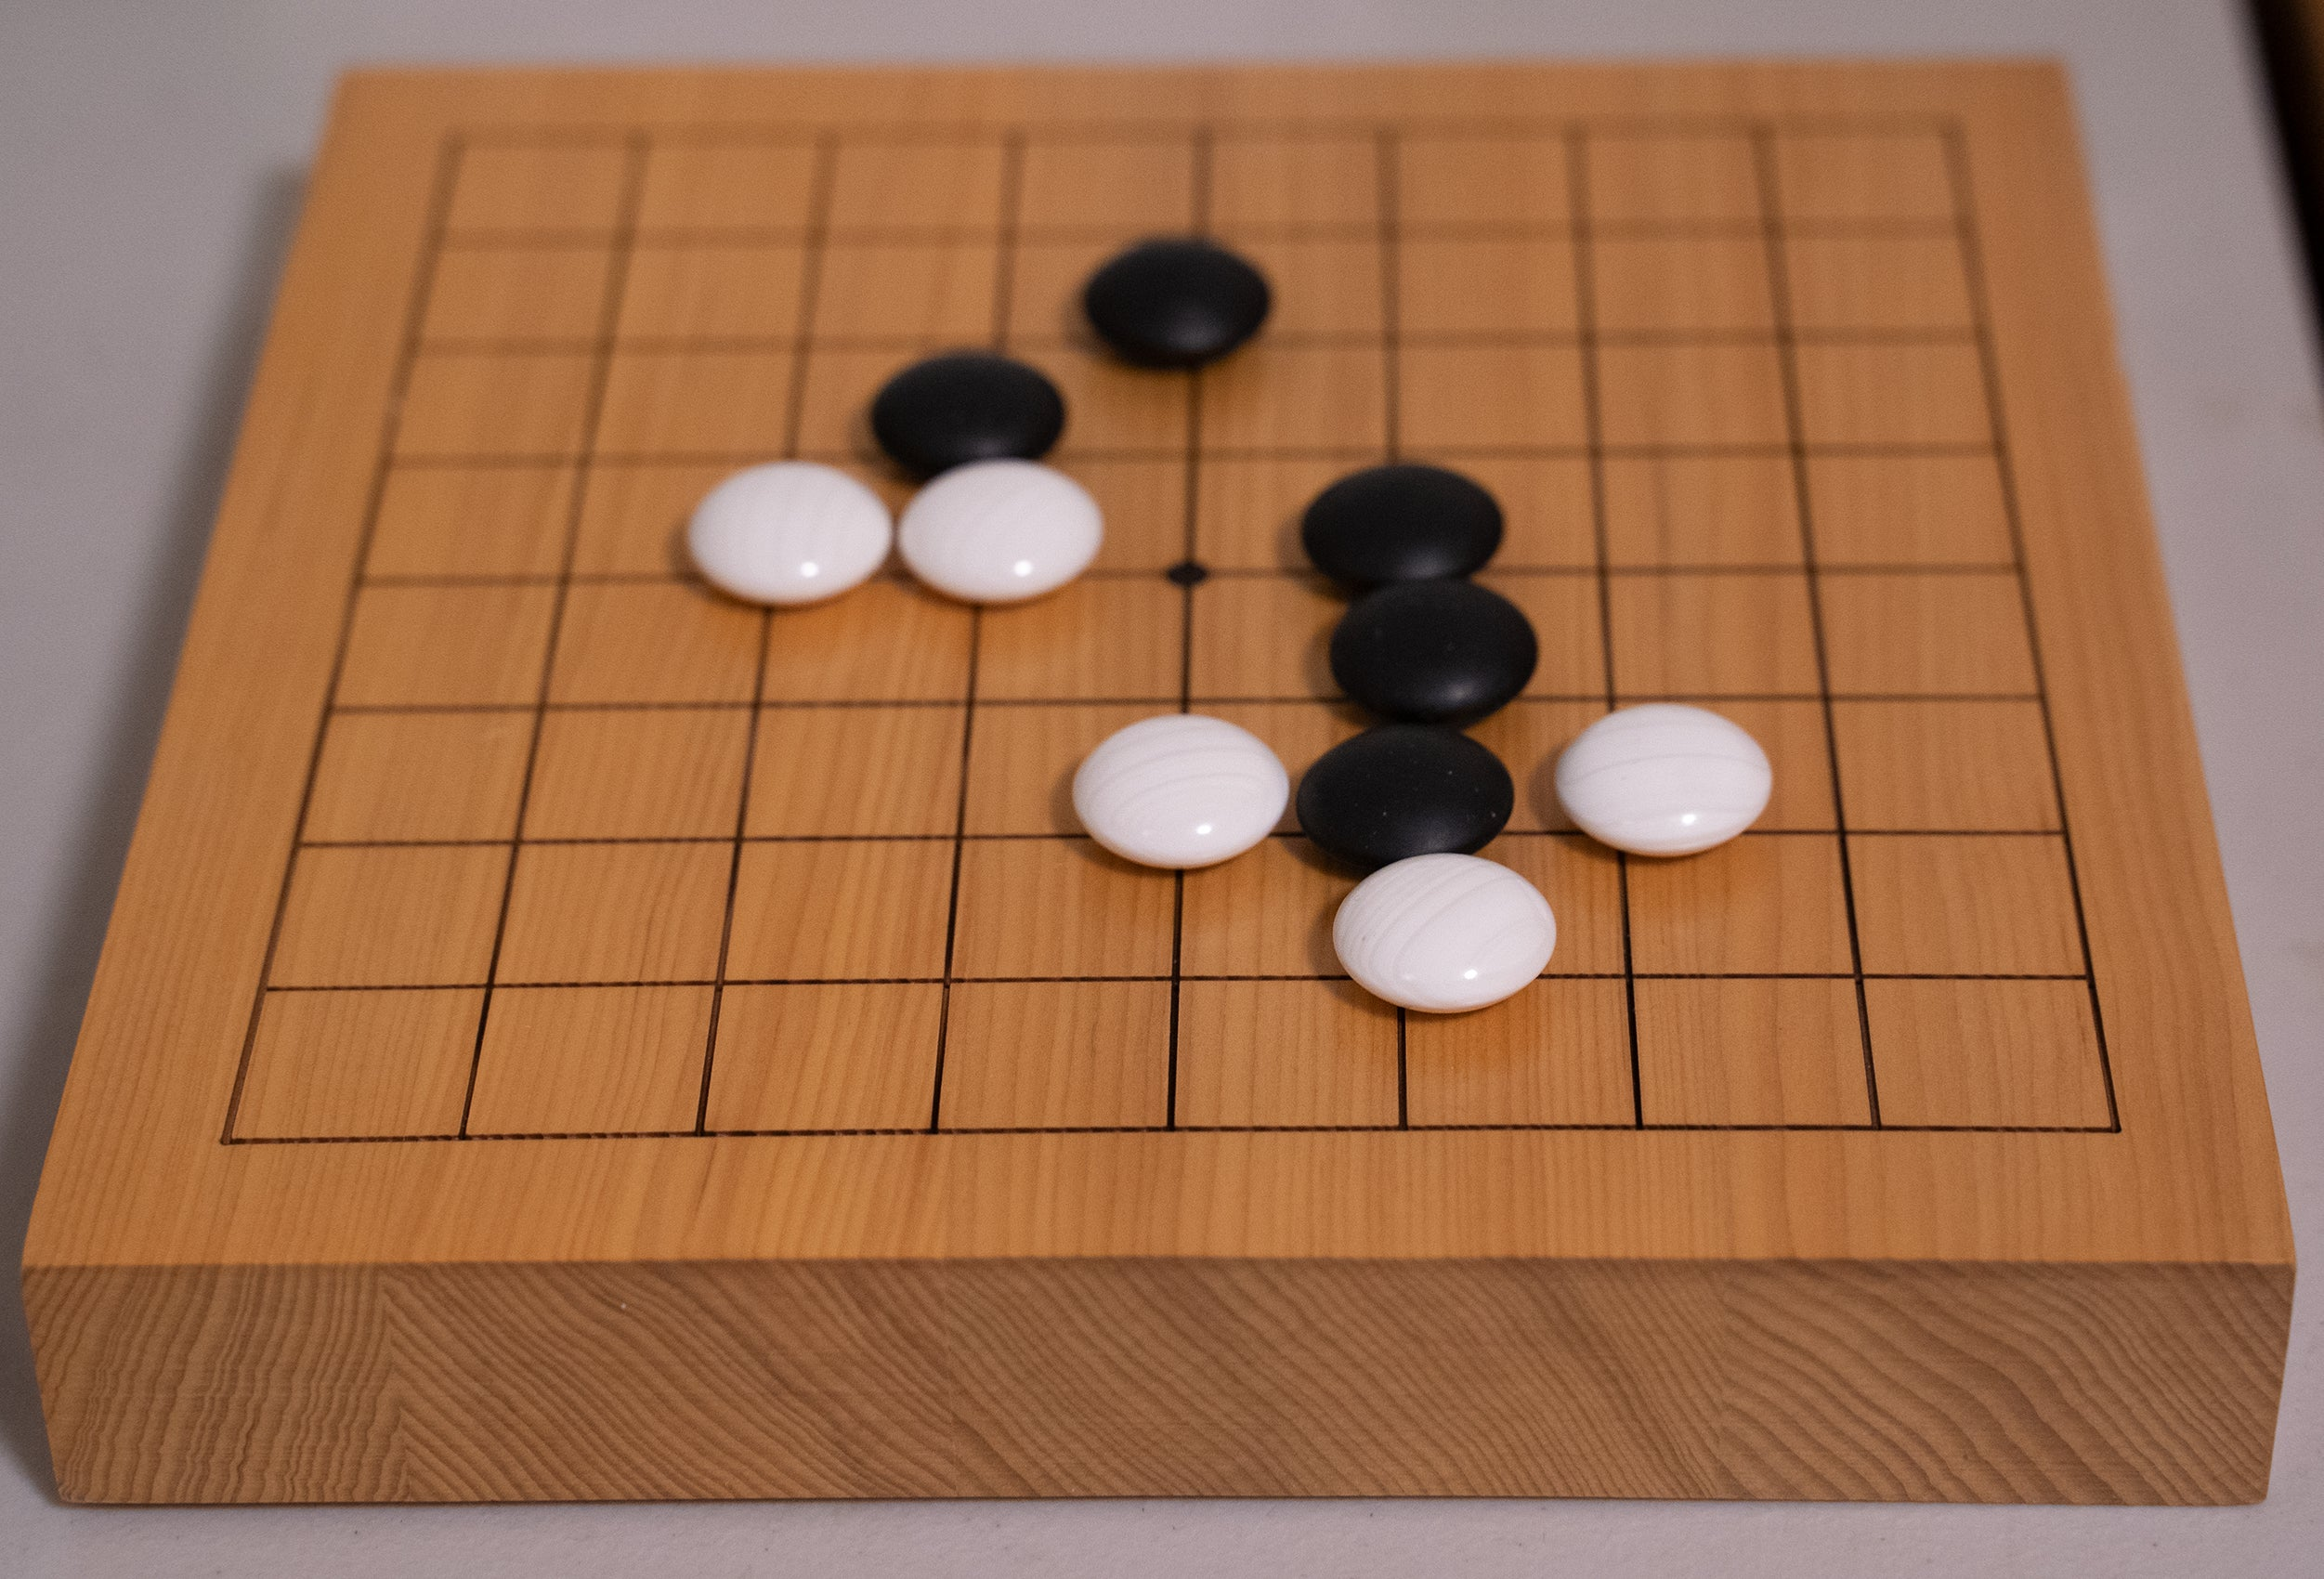
\includegraphics[width=0.38\textwidth]{../tablero.jpg}
	\caption{Tablero de go de dimensiones $9\times9$. Se muestra un juego, luego de cinco movimientos por jugador.}
	\label{fig:tablero}
\end{wrapfigure}

Como podemos observar, se cuenta con dos colores de fichas, blancas y negras, siendo un color por jugador.
A diferencia del ajedrez, las fichas de un jugador son indistinguibles y una vez jugadas no se pueden volver a mover.
Se puede capturar una piedra o un conjunto de piedras y eliminarlas del tablero si est\'an completamente rodeadas por piedras de otro color.
Uno de los objetivos principales es la de formar territorios.
Estos son zonas del tablero en el cual est\'an dominados por un jugador, sin posibilidad de perderlos ante el rival.
De modo resumido, al final de la partida, gana el jugador con mayor territorio y fichas capturadas.



A pesar de tener reglas sencillas, el go presenta una complejidad igual o superior al ajedrez debido a la diversidad de jugadas posibles en cada movimiento, requiriendo de una estrategia compleja. %\cite{go3,go4}.
El juego consiste en acumular puntos al final de la partida, mediante la captura de piedras ajenas, y la captura de territorio.
En el juego de go, existen tres formas de victoria.
El jugador que obtenga mayor cantidad de puntos al finalizar la partida, es el ganador.
La segunda forma, y quiz\'as la m\'as obvia, es por el abandono de uno de los dos jugadores.
En general esto sucede, cuando uno de los dos jugadores, toma noci\'on de que no puede ganar la partida por puntos.
Por \'ultimo, es por ausencia de tiempo, el cual, similar al ajedrez, cada jugador cuenta con determinado tiempo el cual se consume en el turno de dicho jugador.

En un juego de go, el jugador con fichas negras (jugador negro), es el que comienza el juego, poniendo la primera ficha en el tablero.
Como el hecho de iniciar la partida, permite estar siempre una jugada adelante que el jugador con fichas blancas (jugador blanco), existe una regla, llamada regla del \textbf{Komi}, la cual, en su mayor\'ia de veces, le asigna al jugador blanco, un n\'umero de puntos para el conteo final, para contrarrestar esta ventaja que tiene el jugador negro.
Estos puntos no tienen ninguna influencia en el juego hasta que esta haya terminado y se cuenten los puntos totales.
Los puntos por \emph{komi} no tiene un valor aceptado a nivel mundial, teniendo cada zona un diferente valor.
A su vez, como se suele jugar sin la posibilidad de empate, para evitarla, se usa un valor de \emph{komi} no entero.
El valor de mayor uso es el de $6.5$.
En muchos otros casos, se utiliza el \emph{komi} de $0.5$, el cual simplemente evita el empate, pero no asigna una ventaja al blanco por el hecho de jugar segundo.


Este juego posee un sistema de clasificaci\'on de los jugadores muy caracterizado, teniendo un sistema de rangos(jerarqu\'ia) de \textit{Kyu} (la inferior) y \textit{Dan} (la superior), similar al sistema caracter\'istico de las artes marciales. Estos niveles van del \textit{Kyu} 30 al \textit{Kyu} 1 y luego del \textit{Dan} 1 al \textit{Dan} 9, ordenados de principiante a maestro.

El go, tiene un sistema para poder equilibrar las partidas, cuando la diferencia de rango entre los dos jugadores es muy grande.
Este es el concepto de \textbf{handicap}, el de dar ventaja a un jugador sobre otro.
En general, se asigna con las fichas negras al jugador de menor rango (habilidad), y dependiendo la diferencia de rango, este jugador inicia el juego con una determinada de fichas m\'as en el tablero.
Es decir, si un jugador en una determinada partida, tiene un \texttt{handicap} de 2, esto representa, que adem\'as de iniciar la partida con una ficha, este tiene una ficha adicional en el primer movimiento.
Si tiene \texttt{handicap} 5, adem\'as  de su primer ficha en su primer movimiento, este tiene un adicional de 4 fichas, en esta primera instancia.
En general, estos casos se suele utilizar el valor de \emph{komi} de $0.5$ y ademas estas fichas de \texttt{handicap} tienen una posici\'on asignada fija.

Tanto el \texttt{komi} como el \texttt{handicap}, son conceptos independientes.
Uno representa la ventaja al jugador blanco por iniciar segundo la partida, como tambi\'en imposibilitar el empate.
El otro representa la ventaja al jugador de menor habilidad.
Como ya se menciono, el problema sigue estando en encontrar una escala de valores, en el cual se pueda encontrar el valor ideal para el \texttt{komi}.
Adem\'as esta escala tiene que poder representar al \texttt{handicap} de manera tal, que dado dos jugadores con diferente valor de habilidad, se pueda asignar la ventaja \'optima.
En caso que podamos generar un sistema de habilidad, el cual una diferencia de un punto entre dos jugadores equivale una diferencia en 1 ficha, esto simplificar\'ia el uso de \texttt{handicap}, pudiendo asignar en cada partida el \texttt{handicap} ideal.







\subsection{TrueSkill}
En el marco de las comunidades de juegos en l\'inea, como as\'i en las \'areas de la educaci\'on, deportes, entre otras, una de las caracter\'isticas principales es el concepto de \textbf{habilidad}.
Esta es la cuantificaci\'on de la noci\'on de que tan bueno, o que tan apto es un agente en comparaci\'on a otros, en realizar una actividad en particular.
En contexto de juegos en l\'inea, la habilidad representa que tan bien juega a un determinado juego un agente de la comunidad en relaci\'on al resto.

Uno de los beneficios de poder conocer la habilidad es que nos permite poder hacer un seguimiento respecto a c\'omo fue evolucionando temporalmente.
Esto se consigue mediante el an\'alisis de la informaci\'on de cada agente a lo largo del tiempo.
Si adem\'as se cuenta con informaci\'on de factores externos, podr\'iamos deducir e inferir diversas variables ocultas.
A su vez, permite evitar exponer a los agentes (jugadores miembros de la comunidad en l\'inea) a desaf\'ios desproporcionados, proponiendo partidos o encuentros dentro de un nivel que le resulte desafiante al agente, pero ni demasiado f\'acil ni dif\'icil.

Una de las dificultades radica en que la habilidad es una variable en la cual generalmente es imposible de medir directamente (i.e. variable oculta).
En la pr\'actica, lo mejor que podemos hacer es estimarla a partir de sus consecuencias observables m\'as directas.
Para ello se requiere realizar una serie de suposiciones y generar un modelo, en el cual se pueda representar la realidad deseada.
Una soluci\'on ingenua como observar la frecuencia de resultados positivos (victorias de un jugador), no es un buen indicador, debido a que fundamentalmente depende tambi\'en de la dificultad de los desaf\'ios (habilidad del contrincante).
Por esa raz\'on, todos los modelos convencionales se basan en \emph{pairwise comparisons}.
Ya los primeros modelos generativos, propuestos hace casi un siglo por~\cite{thurstone1927-comparativeJugement} y~\cite{Zermelo1929}, suponen que la probabilidad de un resultado observado, $r_{ij}$, entre un jugador $i$ en contra de un jugador $j$ es $p(\,r_{ij} \,|\, d_{ij}\,)$ la cual depende de la diferencia, $d_{ij}$, entre el agente $i$ y su contrincante $j$.
%decir algo de item responce Theory
El campo se revitaliz\'o 20 a\~nos despu\'es gracias a las publicaciones de \cite{bradley1952} y~\cite{mosteller1951a}.
Actualmente, los estimadores de habilidades m\'as utilizados son los propuestos por~\cite{elo1961-uscf,glikman_gliko_2,Herbrich2007} y algunas de las variantes de la \emph{Item-Response Theory} recopiladas por~\cite{vanDerLinden2016,fox2010}.
Notablemente, todos comparten el mismo modelo generativo subyacente.
Un gran avance produjo la metodolog\'ia desarrollada por~\cite{elo1961-uscf} para la Federaci\'on de Ajedrez de los Estados Unidos (USCF), adoptada hasta el d\'ia de hoy por la Federaci\'on Internacional de Ajedrez (FIDE).

\begin{wrapfigure}{R}{0.4\textwidth}
	\footnotesize
	\tikz{
		\node[det, fill=black!10] (r) {$r_{ij}$} ;
		\node[const, left=of r, xshift=-1.35cm] (r_name) {\footnotesize Resultado:};
		\node[const, right=of r] (dr) {\footnotesize $ r_{ij} = (d_{ij}>0)$};

		\node[latent, above=of r, yshift=-0.45cm] (d) {$d_{ij}$} ; %
		\node[const, right=of d] (dd) {\footnotesize $ d_{ij}=p_i-p_j$};
		\node[const, left=of d, xshift=-1.35cm] (d_name) {\footnotesize Diferencia:};

		\node[latent, above=of d, xshift=-0.8cm, yshift=-0.45cm] (p1) {$p_i$} ; %
		\node[latent, above=of d, xshift=0.8cm, yshift=-0.45cm] (p2) {$p_j$} ; %
		\node[const, left=of p1, xshift=-0.55cm] (p_name) {\footnotesize Rendimiento:};

		\node[accion, above=of p1,yshift=0.3cm] (s1) {} ; %
		\node[const, right=of s1] (ds1) {$s_i$};
		\node[accion, above=of p2,yshift=0.3cm] (s2) {} ; %
		\node[const, right=of s2] (ds2) {$s_j$};

		\node[const, right=of p2] (dp2) {\footnotesize $p \sim \N(s,\beta^2)$};

		\node[const, left=of s1, xshift=-.85cm] (s_name) {\footnotesize Habilidad:};

		\edge {d} {r};
		\edge {p1,p2} {d};
		\edge {s1} {p1};
		\edge {s2} {p2};
		%\node[invisible, right=of p2, xshift=4.35cm] (s-dist) {};
	}
	\caption{Modelo generativo: las habilidades ocultas causan resultados observables a trav\'es de los rendimientos aleatorios.}
	\label{fig:generative_model}
\end{wrapfigure}

La figura~\ref{fig:generative_model} ofrece una representaci\'on gr\'afica en la que las habilidades ocultas generan los resultados observables.
La relaci\'on causal no es directa.
Si bien los agentes pueden tener una habilidad espec\'ifica en cada momento ($s_i$ y $s_j$), el desempe\~no ($p_i$ y $p_j$) que exhiben en cada evento depende de una cantidad indeterminada de factores desconocidos, que se modelan como un ruido aleatorio gaussiano alrededor de la media ($s_i$ y $s_j$) expresado como $\N(p\,|\,s,\beta^2)$ para cada uno de los agentes.
Seg\'un este modelo, los resultados son una consecuencias directa de la diferencia de esos rendimientos ocultos, $d_{ij}=p_i - p_j$.
Un agente obtiene un resultado positivo cuando supera el rendimiento de su adversario, $r_{ij} = (d_{ij} > 0)$.
Al observar un resultado podemos deducir, dadas las hip\'otesis, el orden de los rendimientos ocultos que, en efecto, ocurri\'o en ese evento, y su probabilidad a priori.
La soluci\'on metodol\'ogica de \texttt{Elo} es extremadamente sencilla y astuta: actualizar la estimaci\'on actual de habilidad en funci\'on de la sorpresa del resultado, actualizando m\'as fuertemente la estimaci\'on cuanto mayor es la diferencia entre los jugadores, favoreciendo el caso en el que gana el menos probable.

Esta soluci\'on puede recuperar la escala relativa de los agentes, partiendo de valores iniciales arbitrarios.
Sin embargo, tiene algunas debilidades importantes.
Debido a la falta de una noci\'on de incertidumbre sobre las estimaciones, lo que un agente pierde en habilidad lo adquiere el otro.
Como las estimaciones sobre nuevos jugadores (poco conocidos al momento) tienden a generar alta sorpresa, su presencia puede modificar las estimaciones bruscamente.
Una soluci\'on ad-hoc fue propuesta para romper esta simetr\'ia del modelo de \texttt{Elo}, que consiste en reducir el impacto de la actualizaci\'on mediante la multiplicaci\'on de una constante en funci\'on de las veces que el agente ya fue visto por el sistema.

La Teor\'ia de la Probabilidad nos proporciona un marco consistente para cuantificar la incertidumbre de nuestras creencias~\cite{bishop2006-PRML}, posibilitando una opci\'on para no agregar a nuestro modelo soluciones ad-hoc.
Al proceso de computar distribuciones de probabilidad luego de observar el valor de alguna variable aleatoria se llama \textbf{inferencia}.
El uso de la teor\'ia de la probabilidad para manejar la incertidumbre, conocida como inferencia bayesiana, est\'a hoy adoptada de manera generalizada en el \'ambito de la inteligencia artificial y el aprendizaje autom\'atico fundamentalmente porque ha mostrado ser un instrumento sumamente \'util en la pr\'actica.

Cualquier sistema que represente grados de creencia mediante un valor num\'erico, consistente con la l\'ogica deductiva cl\'asica y un conjunto de axiomas que codifican el razonamiento de sentido com\'un, ser\'a necesariamente isom\'orfico a la teor\'ia de la probabilidad~\cite{Cox1946,vanHorn2003}.

% introduccion a trueskill
En el 2006, Herbrich~\cite{Herbrich2007} propuso un m\'etodo probabil\'istico, denominado \texttt{TrueSkill}, en el cual solucionaba varias de las limitaciones de \texttt{Elo}.
A diferencia de \texttt{Elo}, que considera a la habilidad como un \'unico escalar, \'este la modela con una distribuci\'on gaussiana, teniendo as\'i la media de la distribuci\'on como la habilidad m\'as probable, y a la desviaci\'on est\'andar como la incerteza que se tiene.
A su vez, al igual que \texttt{Elo}, supone un rendimiento $p$, el cual el jugador con mayor valor es el ganador.
De esta forma, observando el resultado en un juego dado, el m\'etodo de \texttt{TrueSkill}, actualiza la distribuci\'on de habilidad.
Mientras m\'as informaci\'on tengamos de un jugador (mayor n\'umero de partidas), mayor certeza tendremos de su habilidad.
Es decir, es imprescindible contar con un gran volumen de informaci\'on con el fin de reducir nuestra incertidumbre en la habilidad de cada jugador, logrando estimaciones m\'as certeras.


\subsection{TTT}


El algoritmo de \texttt{TrueSkill}, presenta algunas limitaciones importantes.
Por un lado, la inferencia que se realiza en un determinado rango temporal t, depende del orden de como se eligen los eventos para su actualizaci\'on.
Dado que no se asume ning\'un conocimiento sobre los resultados del evento dentro de un rango temporal dado, los resultados de la inferencia debe ser independiente del orden de los juegos dentro de ese rango temporal.
Adem\'as, una limitaci\'on se debe a que la informaci\'on solo se propaga temporalmente en un sentido.
Esto es una desventaja, debido a que en muchos casos, no se aprovecha toda la informaci\'on de un evento.
En concreto, si un dado jugador A le gana a un dado jugador B y luego resulta ser que este segundo jugador resulta ser muy bueno (una habilidad muy grande), \texttt{TrueSkill} no es capaz de propagar esta informaci\'on al pasado y corregir la habilidad del jugador A.

Ambos problemas son resueltos al extender el filtro de densidad gaussiana, para correr de manera completa \texttt{expectation propagation}~\cite{herbrich2005}, hasta converger, denominado \texttt{TrueSkill Through Time}.
La idea b\'asica es actualizar repetidamente el mismo evento asegurando que el efecto de la actualizaci\'on previa de ese resultado sea removida antes de que el nuevo efecto se agregue.
De esta manera el modelo se mantiene igual pero la inferencia est\'an menos aproximadas.

Un ejemplo sencillo y conceptualmente importante, es el caso de tres jugadores donde cada uno gana y pierde una partida entre ellos.
Imag\'inese 3 jugadores, \texttt{a},\texttt{b} y \texttt{c}, en donde en un mismo d\'ia el jugador \texttt{a} le gana una partida al jugador \texttt{b}, luego \texttt{b} le gana una partida al jugador \texttt{c} y por ultimo \texttt{c} gana una partida al jugador \texttt{a}.
Podemos intuir que la respuesta que buscamos, es que si no ten\'iamos informaci\'on previa de ning\'un jugador, cada jugador gano y perdi\'o un juego, y por ende deber\'ian finalizar con una misma estimaci\'on de habilidad.
\texttt{TrueSkill} al importar el orden en como estima, luego de la primer partida, supondr\'ia que el jugador \texttt{a} es superior a \texttt{b}, asignando a este ultimo menor habilidad.
Luego este jugar\'ia contra \texttt{c}, que al perder supondr\'ia que este ultimo es aun peor.
Por ultimo, en la ultima partida, se tendr\'ia un caso de que un jugador que se supone muy malo (\texttt{c}), le gana a un jugador que se supone muy bueno (\texttt{a}).
Esto conlleva a que los tres jugadores finalicen con habilidades diferentes.
Utilizando \texttt{TrueSkill Through Time} en el ejemplo reci\'en contado los tres jugadores finalizan con la misma habilidad estimada.




%%%%%%%%%%%%%%%%%%%%%%%%%%%%%%%%%%%%%%%%%%%%%%%%%%%%%%%%%%%%%%%%%%%%%%%%%%%%%%%
% Modelos
%%%%%%%%%%%%%%%%%%%%%%%%%%%%%%%%%%%%%%%%%%%%%%%%%%%%%%%%%%%%%%%%%%%%%%%%%%%%%%%
\chapter{Fundamentos}



Este cap\'itulo se encuentra divido en dos partes.
En la primer secci\'on veremos los fundamentos necesarios para entender el m\'etodo gr\'afico probabil\'istico de \texttt{TrueSkill}.
Primero veremos un modelo probabil\'istico bayesiano el cual es usado como marco de referencia.
Luego veremos algunas propiedades de las distribuciones gaussiana que resultan fundamentales para el m\'etodo en cuestion.
A su vez veremos algunos conceptos como los gr\'aficos de factores, pasaje de mensajes, aproximaciones utilizadas, m\'etrica de evaluaci\'on y m\'as.
Se finaliza explicando el funcionamiento de \texttt{TrueSkill} y del sucesor \texttt{TrueSkill Through Time}, utilizado en esta tesis.
Por \'ultimo se realiza un breve ejemplo detallado del las cuentas del primer m\'etodo, el cual es utiliza todo lo necesario para lograr entender a estos m\'etodos.


Si el lector cuenta con conocimientos de probabilidad y estad\'istica, puede avanzar a la secci\'on~\ref{Sec:Modelos} (\nameref{Sec:Modelos}).
En particular, la secci\'on~\ref{Sec:ModeloProbalistico} (\nameref{Sec:ModeloProbalistico}) y \ref{Sec:PropiedadesGaussianas} (\nameref{Sec:PropiedadesGaussianas}) se consideran conocimientos b\'asicos.


En la segunda secci\'on veremos algunos de los diversos tipos de m\'etodos y modelos predictivos existentes para estimar e inferir alguna variable oculta.
En lo que concierne a esta tesis, nos centraremos en los modelos de habilidad en juegos y deportes.
En particular en el m\'etodo \texttt{TrueSkill Through Time} y sus predecesores para contextualizar.

\section{Introducci\'on te\'orica}
%%%%%%%%%%%%%%%%%%%%%%%%%%%%%%%%%%%%%%%%%%%%%%%%%%%%%%%%%%%%%%%%%%%%%%%%
%%%%%%%%%%%%%%%%%%
%%%%%%%%%%%%%%%%%%%%%%%%%%%%%%%%%%%%%%%%%%%%%%%%%%%%%%%%%%%%%%%%%%%%%%%%



\subsection{Modelo probabil\'istico}\label{Sec:ModeloProbalistico}

Uno de los primeros desaf\'ios que se tiene es poder ser capaces de manejar cantidades en las cuales desconocemos su valor.
De hecho, la necesidad de lidiar con la incertidumbre surge en nuestro mundo cada vez m\'as basado en datos.
En el caso de \texttt{TrueSkill}, cuando empezamos a estimar la habilidad de un nuevo jugador, arrancamos con una creencia con mucha incertidumbre (debido a que no tenemos informaci\'on sobre \'este) y a medida que va jugando las diferentes partidas del juego, se va induciendo su habilidad reduciendo su incertidumbre.
En esta clase de juegos, siempre es m\'as probable que el jugador m\'as fuerte sea el ganador, aunque \'esto no est\'a garantizado.
El uso de sistemas de referencias probabil\'isticos nos permite cuantificar estas cantidades inciertas con alg\'un grado de incertidumbre.

La probabilidad asociada a un suceso o evento aleatorio es una medida del grado de certidumbre de que dicho suceso ocurra.
Los diferentes valores que se pueden dar en esta  clase de eventos se conoce como variables aleatorias.
Utilizaremos la notaci\'on est\'andar, donde la $p$ min\'uscula es la densidad de probabilidad de una variable continua, y la $P$ may\'uscula para denotar la distribuci\'on de probabilidad de una variable discreta.
Representaremos con $x$ e $y$ a dos variables aleatorias.

Existen diferentes distribuciones de importancia para esta tesis.
A la distribuci\'on en donde la variable aleatoria tiene solo dos valores, se la conoce como distribuci\'on de \textbf{Bernoulli} o bien como \textbf{funci\'on indicadora} ($\mathbb{I}$).
En los casos en donde se tiene absoluta certeza de la variable de dos estados (i.e. probabilidad del \SI{100}{\percent}),  se lo conoce como \textbf{punto de masa}.
En general, esto \'ultimo se utiliza cuando se observa una variable, conociendo as\'i su valor real.
La probabilidad condicional, $P(x|y)$, es la probabilidad de que suceda un evento dado que tenemos informaci\'on a partir de otra variable $y$.
Se dice que dos variables son \textbf{independientes} si vale que $P(x|y) = P(x)$.
En caso contrario, se las denomina como variables \textbf{dependientes}.
El concepto de independencia es importante para este tipo de modelos, ya que cualquier variable no incluida expl\'icitamente en nuestro modelo se supone que es independiente a todas las otras variables.
Es importante observar que la suma de los posibles valores de la variable condicionada $x$ se encuentra normalizada, pero no as\'i la suma con los valores posibles de la variable $y$.
Se conoce como \textbf{probabilidad conjunta}, a la probabilidad de que dos o m\'as variables aleatorias tengan un determinado valor, $P(x,y)$.
Realizar la suma de todas las variables excepto una ( en este caso, $x$), se lo conoce como \textbf{marginalizaci\'on} de la variable $x$, y da como resultado la probabilidad de esta variable.

\begin{equation} \label{eq:sum_rule}
\tag{regla de la suma}
P(x) = \sum_{y \in Y} P(x,y) \ \ \ \ \ \text{o} \ \ \ \ \ p(x) = \int p(x,y) \, dy
\end{equation}

Esto significa que cualquier distribuci\'on marginal $P(x)$ puede ser obtenida integrando la distribuci\'on conjunta $P(x,y)$, en este caso sumando todos los valores de $Y$.
Otra propiedad muy importante de las distribuciones conjuntas es la conocida como regla del producto.
Esta regla relaciona a esta distribuci\'on con la probabilidad condicional y marginal.

\begin{equation}\label{eq:product_rule}
\tag{regla del producto}
P(x,y) = P(x|y) P(y)
\end{equation}

Toda inferencia probabil\'istica, no importa cu\'an compleja ella sea, puede ser resuelta a trav\'es de dos simples ecuaciones: la~\ref{eq:sum_rule} y la~\ref{eq:product_rule}.
Adem\'as, cualquier distribuci\'on conjunta puede ser expresada como el producto de distribuciones condicionales uni-dimensionles.
Utilizando esta regla junto con la propiedad de simetr\'ia $P(x,y) = P(y,x)$, se obtiene inmediatamente el~\ref{eq:bayes_theorem}.
%
\begin{equation}\label{eq:bayes_theorem}
\tag{teorema de Bayes}
P(y|x) = \frac{P(x|y)P(y)}{P(x)}
\end{equation}
%

Se conoce como modelo bayesiano, a un modelo estad\'istico en donde se utilizan probabilidades para representar todas las incertidumbres dentro de nuestro modelo, tanto las incertezas de entrada como de salida.
En este tipo de modelos, se utilizan los conceptos de distribuciones de probabilidad a priori y a posteriori.
Es decir, poder usar teor\'ia probabil\'istica para representar nuestro conocimiento de alguna variable aleatoria, conocida como \textbf{prior} y luego de obtener nueva informaci\'on, poder hacer inferencia, y actualizar esta distribuci\'on a la cual se la denomina \textbf{posterior}.
El uso inferencial del teorema de Bayes juega un rol central en las t\'ecnicas modernas de aprendizaje estad\'istico.
Esta expresi\'on nos permite actualizar nuestras creencias sobre ciertas hip\'otesis, dado un modelo y los datos.
Para reducir la incertidumbre sobre la habilidad oculta utilizando la informaci\'on provista por el resultado observado y por el modelo causal descripto, se requiere resolver la siguiente ecuaci\'on,

\begin{equation}\label{eq:inference}
\underbrace{p(\overbrace{\text{Skills}}^{Hidden}|\overbrace{\text{Result,Model}}^{Observed})}_{\text{Posterior}} = \frac{\overbrace{P(\text{Result}|\text{Skills,Model})}^{\text{likelihood}}\overbrace{p(\text{Skills})}^{\text{Prior}}}{\underbrace{P(\text{Result}|\text{Mode})}_{\text{Evidence}}}
\end{equation}

donde el lugar que ocupa el modelo queda impl\'icito.
Se conoce como la funci\'on \textit{likelihood}  a la medida de la bondad del ajuste de nuestro modelo luego de haber inferido con una muestra de datos (resultado de un juego) para valores dados de las variables desconocidas (habilidad de los jugadores, \textit{skill}).
En nuestro caso, la hip\'otesis es el valor de la habilidad a priori de los jugadores en un determinado evento y el dato es el resultado de dicho juego (\textit{result}).
La evidencia es simplemente una constante de normalizaci\'on, para que la probabilidad a posteriori lo est\'e.




\subsection{Distribuci\'on gaussiana}\label{Sec:PropiedadesGaussianas}

El m\'etodo de \texttt{TrueSkill} se puede utilizar para obtener estimaciones de la habilidad y otras variables con distribuciones gaussianas.
En teor\'ia de probabilidad, la distribuci\'on gaussiana, o tambi\'en conocida como distribuci\'on normal, es un tipo de distribuci\'on de probabilidad continua para una variable aleatoria de valor real.
Este tipo de distribuci\'on resulta muy \'util debido a su simplicidad. 
Solamente, es necesario utilizar dos par\'ametros para describirla: la media ($\mu$) y la desviaci\'on est\'andar ($\sigma$).
La primera representa el valor m\'as probable de la variable aleatoria, y la desviaci\'on est\'andar representa la incerteza que se tiene sobre este valor.
A su vez, estas distribuciones poseen diversas propiedades matem\'aticas que facilitan su manipulaci\'on algebraica, especialmente cuando se trabaja con m\'ultiples distribuciones gaussianas.
Su forma general est\'a dada por,

\begin{equation}
N(x|\mu, \sigma^2)=\frac{1}{\sigma\sqrt{2\pi}}\exp^{-\frac{1}{2}\left(\frac{x-\mu}{\sigma}\right)^2} \label{ec:gauss}
\end{equation}

Donde la notaci\'on muestra la variable aleatoria $x$, seguido por los par\'ametros de la distribuci\'on $\mu$ y $\sigma$ (an\'aloga a la notaci\'on $x \sim N(\mu, \sigma^2)$).
El par\'ametro $\mu$ representa la media de la distribuci\'on, mientras que el par\'ametro $\sigma$ la desviaci\'on est\'andar, la cual representa el ancho de la campana.
La figura~\ref{fig:gaus} presenta un esquema gr\'afico de una distribuci\'on normal o gaussiana t\'ipica definida en la ecuaci\'on~\ref{ec:gauss}.

\begin{figure}[H]
	\centering
	\includegraphics[width=0.7\textwidth]{gaussian.pdf}
	\caption{Distribuci\'on normal de media $\mu$ y desviaci\'on est\'andar $\sigma$. Los porcentajes representan el porcentaje de \'area correspondiente al sector sombreado.}
	\label{fig:gaus}
\end{figure}


Esta distribuci\'on esta normalizada y ademas el \'area bajo la curva encerrada en una desviaci\'on est\'andar a cada lado de la media da el \SI{68.2}{\percent} del total.
Por convenci\'on se define a $\sigma^2$ como la varianza.
Existen importantes propiedades que se utilizan para calcular \textit{TrueSkill}, como son la suma y producto entre gaussianas, la funci\'on gaussiana acumulada, entre otras propiedades.
Las demostraciones de estas propiedades se encuentran en el ap\'endice~\ref{appendix:gauss}.%(\nameref{appendix:gauss}). 
Estas distribuciones cuentan con la siguiente simetr\'ia:


\begin{equation}\label{eq:simetria}
N(x|\mu,\sigma^2) = N(\mu|x,\sigma^2) = N(-\mu|-x,\sigma^2) = N(-x|-\mu,\sigma^2)
\end{equation}

La integral de la multiplicaci\'on de dos gaussianas es,

\begin{equation}\label{eq:multiplicacion_normales}
\int_{-\infty}^{\infty} N(x|\mu_x,\sigma_x^2)N(x|\mu_y,\sigma_y^2) \, dx = N(\mu_x|\mu_y,\sigma_x^2+\sigma_y^2)
\end{equation}

Se define como $\Phi(x|\mu,\sigma^2)$ a la funci\'on de acumulada gaussiana.
\'Esta tiene los mismos par\'ametros que la anterior distribuci\'on, integr\'andose desde $-\infty$ hasta $x$.
En la figura~\ref{fig:acumulativa} se puede visualizar una distribuci\'on gaussiana junto con la acumulada para todo $x$.
Esta definida como,


\begin{equation}\label{eq:phi_norm}
 \Phi(x|\mu,\sigma^2) = \int_{-\infty}^{x}N(y|\mu,\sigma^2)dy
\end{equation}


\begin{figure}[H]
	\centering
	\includegraphics[width=0.7\textwidth]{gaussian_cumulative.pdf}
	\caption{La curva azul muestra una distribuci\'on gaussiana con media cero y una desviaci\'on est\'andar de uno. El \'area bajo la curva de esta desde $-\infty$ hasta un punto $x$ es conocido como distribuci\'on gaussiana acumulada y se muestra como una funci\'on de $x$ por la curva roja. Se muestra el valor que tiene esta funci\'on en el valor -1, marcando el \'area integrada de la distribuci\'on gaussiana.}
	\label{fig:acumulativa}
\end{figure}



\subsection{Gr\'afico de factores}


A medida que incrementamos la cantidad de variables aleatorias en nuestro modelo, la visualizaci\'on intuitiva tan sencilla como en el caso de solo dos variables, se acompleja, haci\'endose m\'as complicada la probabilidad conjunta.
Un buen m\'etodo es tomar provecho  de que la mayor\'ia de las distribuciones conjuntas se pueden escribir como un n\'umero finito de t\'erminos o factores (i.e. un n\'umero chico de variables).
Se pueden representar distribuciones conjuntas complejas usando gr\'aficos de factores.
\'Estos muestran los distintos factores que forman la distribuci\'on junto con sus variables.
Se utilizan dos tipos de nodos en estos gr\'aficos.
Por un lado se encuentran los nodos de variables, habiendo uno por cada variable del modelo y el nodo de factor, donde hay uno por cada factor en la distribuci\'on conjunta.
Estos factores tambi\'en se pueden interpretar como partes de la factorizaci\'on de una funci\'on, pudi\'endose aplicar a otros casos.
En general se representan a los nodos de variables como c\'irculos, encerrando el nombre de la variable y como cuadrados negros con una etiqueta del factor, a los nodos de factores.
Se conecta cada factor con los nodos de variables en las cuales \'este depende.

El siguiente ejemplo, figura \ref{graph:FGej1}, se tiene una funci\'on de tres variables, en la cual se puede representar como un \'unico factor, o mediante la factorizaci\'on de \'esta, pudiendo quedar en tres factores. 
Se observa que cada factor est\'a conectado con una l\'inea con cada variable dependiente.
	\begin{equation*}
	f(x,y,z) = (x+y)(y+z)(x+z)
	\end{equation*}
\begin{center}

	\begin{figure}[H]
		\centering
		\begin{subfigure}{.5\textwidth}
			\centering
			\tikz{ %
				\node[latent] (s1) {$x$} ; %
				\node[factor, below=of s1,xshift=-1.4cm] (fp0) {} ;
				\node[factor, below=of s1,xshift=1.4cm] (fp2) {} ;


				\node[latent, below=of fp0,xshift=-.4cm] (p0) {$y$} ; %
				\node[latent, below=of fp2,xshift=.4cm] (p2) {$z$} ; %
				\node[factor, right=of p0, below=of s1, yshift=-1.6cm] (fp1) {} ;
				%\draw[bend right=90] (fs1) arc (s1) node[midway,above]{label};
				%\draw[bend left,->]  (fs1) to node [auto] {Link} (s1);
				\edge[-] {s1} {fp0,fp2};
				\edge[-] {fp0} {p0};
				\edge[-] {fp2} {p2};
				\edge[-] {p0} {fp1};
				\edge[-] {fp1} {p2};

			}
			\caption{}
			\label{graph:FGej1-1}
		\end{subfigure}%
		\begin{subfigure}{.5\textwidth}
			\centering
			\tikz{ %
				\node[latent] (s1) {$x$} ; %
				\node[factor, below=of s1] (fp0) {} ;

				\node[latent, below=of fp0,xshift=-1.4cm] (p0) {$y$} ; %
				\node[latent, below=of fp0,xshift=1.4cm] (p2) {$z$} ; %
				%\draw[bend right=90] (fs1) arc (s1) node[midway,above]{label};
				%\draw[bend left,->]  (fs1) to node [auto] {Link} (s1);
				\edge[-] {s1} {fp0};
				\edge[-] {p0} {fp0};
				\edge[-] {p2} {fp0};
			}
			\caption{}
			\label{graph:FGej1-2}
		\end{subfigure}
		\caption{Se muestra dos formas distintas de representar la funci\'on $f(x,y,z) = (x+y)(y+z)(x+z)$ mediante gr\'aficos de factores. }
		\label{graph:FGej1}
	\end{figure}
\end{center}

Como sabemos, una funci\'on no tiene una \'unica forma de factorizaci\'on, y es por eso que existen diversos gr\'aficos de factores para cada caso.
Se elige el indicado dependiendo del grado de abstracci\'on que se requiera.
En el caso de esta tesis, se utilizaran estos gr\'aficos con la combinaci\'on de inferencia bayesiana.
Veamos un ejemplo en que se requiere estimar un par\'ametro $x$, como puede ser la media de una gaussiana, mediante observaciones independientes $y$, usando inferencia bayesiana, represent\'andolo con un gr\'afico de factores como se observa en figura~\ref{graph:FGej2}. 
Esta estimaci\'on se puede representar algebraicamente utilizando la \ref{eq:product_rule} en donde la distribuci\'on conjunta es igual a el \textit{prior} del par\'ametro $x$, multiplicado por la productoria de los \emph{likelihoods} de cada observaci\'on(probabilidad condicional de $y_i$ dado $x$).
Estamos suponiendo que la distribuci\'on condicional de $y$ es una gaussiana con media $x$ y varianza uno.



\begin{center}
	\begin{equation*}
	\begin{split}
	&p(x,y_1,...,y_n) = p(x)\prod_{i}p(y_i|x) \\
	&p(y_i|x) = N(y_i|x,1)
	\end{split}
	\end{equation*}
	\begin{figure}[H]
		\centering
		\tikz{ %


			\node[factor] (fs1) {} ;
			\node[const, above=of fs1] (nfs1) {$p(x)$}; %

			\node[latent, right=of fs1, xshift=1.25cm, yshift=-1cm,fill=cyan!50] (s1) {$x$} ; %


			\node[factor, below=of s1,xshift=-1.4cm,yshift=-1cm] (fy0) {} ;
			%\node[const, right=of fp0] (nfp0) {$f_{p_i^{t}(1)}$}; %

			\node[factor, below=of s1,yshift=-1cm] (fy1) {} ;
			%\node[const, right=of fp0] (nfp0) {$f_{p_i^{t}(1)}$}; %

			\node[factor, below=of s1,xshift=1.4cm,yshift=-1cm] (fy2) {} ;
			\node[const, right=of fy2] (nfy2) {$p(y_i|x)$}; %

			\node[latent, below=of fy0] (y0) {\footnotesize$y_1$} ; %
			\node[latent, below=of fy1] (y1) {\footnotesize$y_2$} ; %
			\node[latent, below=of fy2] (y2) {\footnotesize$y_3$} ; %

			%\draw[bend right=90] (fs1) arc (s1) node[midway,above]{label};
			%\draw[bend left,->]  (fs1) to node [auto] {Link} (s1);
			\edge[-] {s1} {fy0,fy1,fy2};
			\edge[-] {fy0} {y0};
			\edge[-] {fy1} {y1};
			\edge[-] {fy2} {y2};
			\edge[-] {fs1} {s1};

			\path[draw, -latex, fill=black!50,sloped] (y1) edge[bend right,draw=black!50] node[midway,above,color=black!75, rotate=180] {} (fy1);
			\path[draw, -latex, fill=black!50,sloped] (y2) edge[bend left,draw=black!50] node[midway,below,color=black!75, rotate=180] {} (fy2);
			\path[draw, -latex, fill=black!50,sloped] (y0) edge[bend left,draw=black!50] node[midway,below,color=black!75, rotate=180] { } (fy0);

			\path[draw, -latex, fill=black!50,sloped] (fy1) edge[bend right,draw=black!50] node[midway,below,color=black!75, rotate=180] { } (s1);
			\path[draw, -latex, fill=black!50,sloped] (fy2) edge[bend right,draw=black!50] node[midway,below,color=black!75, rotate=180] { } (s1);
			\path[draw, -latex, fill=black!50,sloped] (fy0) edge[bend left,draw=black!50] node[midway,below,color=black!75, rotate=180] {} (s1);

			\path[draw, -latex, fill=black!50,sloped] (fs1) edge[bend left,draw=black!50] node[midway,below,color=black!75] {}(s1);
		}
		\caption{Representaci\'on grafica por mediante a factores de la estimaci\'on de la media de una distribuci\'on gaussiana. Se sombrea en azul la variable a la cual se esta calculando su marginal.}
		\label{graph:FGej2}
	\end{figure}
\end{center}

Podemos observar un factor que representa el \textit{prior} de $x$, un nodo para dicha variable, y luego un factor por cada \emph{likelihood}.
Se observa la no dependencia de estos factores, ya que solo se conectan con la variable $x$ y no entre s\'i.
Otra de las ventajas de este modelo gr\'afico, es que logra representar de forma gr\'afica el funcionamiento  del algoritmo.
En este ejemplo, cuando inferimos sobre $x$, vemos que los nodos de $y$, env\'ian mensajes a $x$.
Aun con gr\'aficos de factores complejos, siempre la probabilidad conjunta sobre las variables aleatorias (representada por los nodos), puede ser escrita como el producto de los factores (representados por los nodos de factores).
La probabilidad conjunta da una completa especificaci\'on del modelo, ya que define la probabilidad de cualquier posible combinaci\'on de valores para todos las variables aleatorias del modelo.
En el caso de tener el valor de una variable aleatoria, \'este se representa con el nodo de dicha variable sombreada en rojo, para enfatizar que es una variable observada.

Representar un modelo probabil\'istico usando un gr\'afico de factores, trae muchos beneficios.
Provee una manera simple de visualizar la estructura del modelo probabil\'istico y ver que variables tienen influencias entre ellas.
Se puede usar para motivar y dise\~nar nuevos modelos al modificar cambios apropiados al gr\'afico.
Las suposiciones codificadas dentro del modelo pueden ser vistas de manera clara.
Informaci\'on sobre las propiedades de un modelo se pueden obtener mediante operaciones hechas en el gr\'afico.
C\'omputos realizados sobre el modelo pueden ser hechos de manera eficiente por un algoritmo que use la estructura del gr\'afico.



\subsection{Pasaje de mensajes}\label{Sec:PasajeDeMensajes}

Una parte fundamental para poder entender el m\'etodo de \texttt{TrueSkill} m\'as adelante, es el concepto de pasaje de mensajes.
Esto es debido que a medida que nuestros gr\'aficos de factores se acomplejan, como es en el caso reci\'en mencionado, es necesario poder inferir de manera mec\'anica mediante alg\'un algoritmo, de manera \'optima a nivel computo.
Este funciona mediante el pasaje de informaci\'on a trav\'es de los bordes del gr\'afico de factores, donde un mensaje es una distribuci\'on de probabilidad sobre las variables que est\'an conectadas con ese borde.
En nuestro caso usaremos un algoritmo llamado \textbf{sum-product-algorithm}~\cite{Kschischang2001} m\'as bien conocido en el \'area de estad\'istica como \textbf{belief propagation}~\cite{pearl1986-beliefNetworks}, el cual es un algoritmo desarrollado para computar distribuciones marginales posteriores sobre las variables en un gr\'afico de factores en los cuales no tengan ciclos o bucles.
Este algoritmo usa dos tipos de mensajes distintos, uno para el mensaje que va de un factor a una variable,  y otro para los mensajes que van de una variable a un factor.
Las variables observadas env\'ian un mensaje de punto de masa.
Teniendo esto vamos a poder automatizar el calculo de inferencia.

Sea $m_{x \rightarrow f}(x)$ el mensaje enviado por el nodo variable $x$ al nodo factor $f$, y $m_{f \rightarrow x}(x)$ el mensaje enviado por un nodo factor $f$ a un nodo variable $x$.
Denotamos como $n(v)$ al conjunto de nodos vecinos al nodo $v$.
Luego, el primer tipo de mensaje puede ser expresado del siguiente modo,

\begin{equation}\label{eq:m_v_f}
m_{x \rightarrow f}(x) = \prod_{h \in n(x) \setminus \{f\} } m_{h \rightarrow x}(x)
\end{equation}

Es decir todos los mensajes que llegan al nodo $x$ sin contar el que env\'ia el nodo al cual se quiere enviar el mensaje.
El segundo tipo de mensaje puede ser expresado como,

\begin{equation}\label{eq:m_f_v}
m_{f \rightarrow x}(x) = \int \cdots \int \Big( f(\bm{x}) \prod_{h \in n(f) \setminus \{x\} } m_{h \rightarrow f}(h) \Big) \,  d\bm{x}_{\setminus x}
\end{equation}

Donde $\bm{x} = \text{arg}(f)$ es el conjunto de argumentos de la funci\'on $f$.
Este mensaje es parecido al anterior con la diferencia que se multiplica por su factor y se integra por todas las variables exceptuando a la que se est\'a enviando.
Luego, para calcular una marginal cualquiera, se multiplican todos los mensajes que llegan a dicho nodo,
\begin{equation}\label{eq:marginal}
p(x_i) = \prod_{h \in n(x_i)} m_{h \rightarrow x_i}
\end{equation}

El uso de esta \'ultima es de suma importancia para el m\'etodo.
Es la marginal la cual estima la habilidad de los jugadores, mediante la variable de dicho par\'ametro.
Por otro lado, una propiedad en la cual usaremos seguido en los mensajes, son las integrales con una funci\'on indicadora.

\paragraph{Integrales con funci\'on indicadora}
\begin{equation}\label{eq:integral_con_indicadora}
\begin{split}
\int_{-\infty}^{\infty}  \int_{-\infty}^{\infty}  \mathbb{I}(x=h(y,z)) f(x) g(y)\, dx\, dy &=  \int_{-\infty}^{\infty} \int_{h(y,z)}^{h(y,z)} f(h(y,z)) g(y)\, dx\, dy\\
& = \int_{-\infty}^{\infty} f(h(y,z)) g(y) dy
%& \propto \int f(h(y,z)) g(y) dy
\end{split}
\end{equation}

Podemos ver que gracias a esta funci\'on, nos queda una integral de una \'unica variable.


\subsection{Expectation Propagation}
Uno de los inconvenientes con \textbf{belief propagation} es cuando tenemos alg\'un bucle en nuestro gr\'afico de factores.
Para esto se requiere un orden sobre c\'omo y cuando los mensajes se env\'ian.
En particular en las partes en donde se iteran los mensajes hasta su convergencia.
En el caso de \texttt{TrueSkill} se utiliza el m\'etodo de \textbf{Expectation Propagation}~\cite{herbrich2005}, introducido por Tom Minka.
\'Este permite aproximar unos de los mensajes en particular, de modo tal que  la forma funcional del \textit{posterior} sea igual que el del prior.
%Es decir, el algoritmo de \texttt{TrueSkill} hace que tanto el posterior como el priori tenga la misma forma funcional.
La ventaja de preservar la forma funcional de estas distribuciones, es que debido a que el \textit{posterior} de un jugador en \texttt{TrueSkill},  ser\'a el \textit{prior} de la partida siguiente de dicho jugador, lo cual logra conservar la cantidad de par\'ametros de nuestro modelo para describir la habilidad.
En caso contrario, a medida que el algoritmo evolucione con m\'as cantidad de partidas, la forma funcional ira variando, requiriendo cada vez un mayor n\'umero de par\'ametros para poder describir la habilidad, complejizando los c\'omputos.




%\begin{figure}[H]
%	\centering
%	\includegraphics[width=\textwidth]{algo3-1.png}
%	\caption{posiblemente sacarlo}
%	\label{fig:algo3-1}
%\end{figure}


\subsection{Metodolog\'ia de evaluaci\'on}

Un aspecto importante es poder tener alguna forma de medir y comparar los modelos de forma num\'erica.
Para ello se debe elegir una \textbf{m\'etrica de evaluaci\'on} para que mida que tambi\'en bien se est\'an haciendo las estimaciones.
Una m\'etrica com\'un es la probabilidad de los valores reales bajo las distribuciones inferidas.
En el caso de esta tesis, es la probabilidad de que el resultado de una partida suceda, bajo las habilidades a priori estimadas de los jugadores involucrados.
Si la probabilidad del equipo ganador es baja, muestra que las distribuciones a priori no captan la esencia de la realidad.
En caso contrario, aumenta la validez de nuestras creencias.
Esta m\'etrica nos da un numero de qu\'e de la certeza en nuestras estimaciones de estos jugadores en un evento con nuestro modelo.

Podemos obtener un conteo de este n\'umero a lo largo de la base de datos, generando una productoria entre las probabilidades.
A esta productoria se la conoce como \textbf{evidencia}. % parece que la traduccion es prueba, que evidencia es obviousness
Como son probabilidades, el valor m\'aximo de \'esta es uno, representando una eficiencia del 100\% en nuestro modelo.
El valor m\'inimo es cero, representando una nula concordancia entre nuestro modelo y los datos.
En general, conviene trabajar con el logaritmo de la probabilidad, ya que nos genera n\'umeros m\'as manejables cuando la probabilidad es muy baja.
Adem\'as, por propiedades del logaritmo, la productoria se transforma en una suma, lo cual es  computacionalmente m\'as efectivo.
La peor predicci\'on, nos dar\'a una probabilidad de cero, dando $log(p(s_i))=-\infty$.
Como la probabilidad logar\'itmica perfecta es cero, y en un sistema real nunca es perfecto, el logaritmo de la probabilidad, ser\'a siempre en la pr\'actica un valor negativo.
Es por ello, que se utiliza el negativo del logaritmo de la probabilidad, y mientras menor el valor mejor es la predicci\'on del modelo.
La evidencia a utilizar queda como menos la sumatoria de los logaritmos de las probabilidades de ganar de los jugadores ganadores, dividido por la cantidad de partidas, para tener un promedio y un n\'umero m\'as manejable.


\begin{equation}
	\text{evidencia} = -\frac{log(\prod_{i=1}^{N}Prob_i)}{N}
\end{equation}
En general esta m\'etrica penaliza con seguridad las predicciones err\'oneas muy fuertemente, ya que el logaritmo da valores negativos muy grandes cuando la probabilidad de los valores reales es muy cercana a cero.
En particular, \'esto tiene que ser tomado en cuenta cuando tenemos una base de datos en las cuales sus valores contienen un rango de error.
En el caso como el de esta tesis, donde se toman datos reales (si el juego lo gan\'o un jugador/equipo u otro) se considera que no hay error en los datos, haciendo esta m\'etrica muy eficiente.
En la siguiente secci\'on, luego de mostrar las bases del m\'etodo, podremos ver como calcular estas probabilidades y as\'i calcular la evidencia.


\section{Modelos}\label{Sec:Modelos}


\subsection{Elo}
El modelo de ranking de \texttt{Elo}, fue uno de los primeros en crearse. Fue desarrollado por Arpad \texttt{Elo} en 1959 \cite{elo1961-uscf}.
Fue dise\~nado como un sistema de rankeo para el ajedrez, con el objetivo de predecir el resultado de un juego de un jugador contra otro mediante el c\'alculo de la posibilidad de victoria.
En particular, maneja el empate como la mitad de una victoria y la mitad de una derrota, sin predecir la probabilidad de que ocurra un este echo.
La idea central de \texttt{Elo} es modelar la probabilidad del resultado de un juego a trav\'es de las estimaciones de la habilidad de los jugadores representadas con un \'unico n\'umero $s_i$.
Este m\'etodo fue adoptado en 1970 por la Federaci\'on mundial de ajedrez (FIDE).


La habilidad de un jugador es una cantidad incierta.
Una de las suposiciones de \texttt{Elo} es tratar a la habilidad como un \'unico numero donde su valor se actualiza cuando se observa el resultado de un juego.
Dado un resultado de una partida, entendemos que ser\'ia razonable aumentar el valor de habilidad del ganador y disminuir el valor de la habilidad del perdedor.
Lo que no queda claro es cu\'anto hay que ajustar estos valores.
Intuitivamente, podemos pensar lo siguiente, si el jugador que gan\'o posee una habilidad mucho mayor que el de su contrincante, entonces no nos sorprende este resultado, y entonces el cambio de habilidades tendr\'ia que ser relativamente chico.
En cambio,  si la habilidad del jugador ganador fuera significativamente m\'as chica que su rival, entonces el resultado de que este gane, sorprender\'ia mucho y una actualizaci\'on grande estar\'ia justificada.
Es importante entender como el grado de sorpresa nos indica que tan grande debe ser el cambio en la actualizaci\'on de los valores.

El modelo asume que en cada juego cada jugador exhibe un rendimiento, representada como una variable aleatoria normalmente distribuida, $p_i\sim N(s_i,\beta^2)$, centrado en el verdadero valor de habilidad el cual es desconocido con alguna constante de ruido.
Se asume que el jugador que exhibe mayor rendimiento es el ganador.
Bajo estas suposiciones, podemos inferir en cada juego quien tuvo el rendimiento m\'as grande, al observar el resultado real de la partida, (gano/perdio).
Luego, la probabilidad de que el jugador i gane es $P(p_i>p_j|s_i,s_j)=P(p_i-p_j>0|s_i,s_j)$, como se muestra en la figura~\ref{fig:fig6}.

\begin{figure}[H]
	\centering
	\includegraphics[width=\textwidth]{elo_diff.pdf}
	\caption{Probabilidad conjunta del rendimiento de dos jugadores,$i$, $j$ suponiendo que $s_i>s_j$. Todas las l\'ineas paralelas a la diagonal $p_i=p_j$, representan las isobaras de diferencia de  rendimiento $d_{ij}=p_i-p_j$ }
	\label{fig:fig6}
\end{figure}

Las isobaras de diferencia de rendimiento $d_{ij} = p_i-p_j$, son l\'ineas paralelas a la diagonal $p_i=p_j$.
La probabilidad de una cierta diferencia de rendimiento $d_{ij}$ se computa como,

\begin{equation}\label{eq:ProbDiff}
P(d_{ij}|s_i,s_j) = \iint \mathbb{I}(d_{ij}=p_i -p_j) N(p_i|s_i,\beta^2)N(p_j|s_j,\beta^2) \, dp_i \, dp_j
\end{equation}

Bas\'andonos en las propiedades de las gaussianas, se puede mostrar que la diferencia de rendimiento $d_{ij}$, tambi\'en est\'a distribuida normalmente, centrada en la diferencia de la habilidad, con el doble de varianza, como se observa en la figura~\ref{fig:fig7}.

\begin{equation}\label{eq:ProbDiff2}
P(d_{ij}|s_i,s_j) = N(d_{ij}|s_i-s_j,2\beta^2)
\end{equation}

\begin{figure}[H]
	\centering
	\includegraphics[width=\textwidth]{elo_diff_gauss.pdf}
	\caption{La probabilidad del resultado de un juego bajo la suposici\'on del sistema de Ranking de Elo con $s_i>s_j$. El \'area bajo la curva en el intervalo positivo ($d_{ij}$) es la probabilidad de que el jugador $i$ gane, y el \'area bajo la curva en el intervalo negativo es la probabilidad de que el jugador $j$ gane.}
	\label{fig:fig7}
\end{figure}

Esto reduce el problema de computar la probabilidad del resultado del juego a un problema unidimensional relacionado a la diferencia de rendimiento.
Sea el resultado del juego $r_{ij} = \mathbb{I}(d_{ij}>0)$.
Se puede computar la probabilidad de que el jugador $i$ sea el ganador, $r_{ij} = 0$ ($r_{ij} = 1$ en caso contrario), como,

\begin{equation}
P(r_{ij}=0|s_i,s_j) = P(d_{ij} > 0 | s_i, s_j) = 1 - \Phi \left( \frac{0 - (s_i - s_j)}{\sqrt{2}\beta} \right) \overset{*}{=} \Phi \left(\frac{s_i - s_j}{\sqrt{2}\beta} \right)
\end{equation}

Donde $\Phi$ es la funci\'on de distribuci\'on acumulada de la distribuci\'on normal est\'andar, $N(0, 1)$.
La igualdad destacada ($\overset{*}{=}$), se deriva de la simetr\'ia que tienen las funci\'on de densidad normal.
Luego, la probabilidad del resultado se puede escribir de la siguiente manera,
\begin{equation}
P(r_{ij}|s_i,s_j) = (r_{ij}) P(r_{ij}=0|s_i,s_j) +  (1-r_{ij})P(r_{ij}=1|s_i,s_j)
\end{equation}

Con esto podemos calcular la probabilidad de un resultado dadas las estimaciones de la habilidad $ (s_i, s_j) $.
% Luego de esto tenemos una referencia para actualizarlas.
% Observando un resultado muy poco probable, indicar\'ia que las estimaciones de la habilidad est\'an lejos de ser correctas y deber\'ian ser actualizadas fuertemente para que el resultado observado sea esperado.
% Se define el sentido y grado de actualizaci\'on como,
La soluci\'on metodologica es extramadamente simple y astuta: se empieza con una estimaci\'on arbitraria y luego de ver nueva informaci\'on se actualizan en base a la sorpresa generada por el resultado (i.e. un jugador d\'ebil le gana al mejor).
La predicci\'on a priori inducida por la estimaci\'on previa $s_i$ y $s_j$, definen la sorpresa generada,

\begin{equation}
\Delta_i = \underbrace{y_{ij}}_{\hfrac{\text{Direction}}{\text{(Outcome)}}}\underbrace{\left(1-P(r_{ij}|s_i,s_j)\right)}_{\hfrac{\text{Magnitud}}{\text{(Outcome Surprise)}}}
\end{equation}

Donde $\Delta_i$ es la sorpresa generada, $y_{ij}$ es 1 si el agente $i$ es el ganador y -1 en caso contrario, definido como $y_{ij} =  2\,r_{ij} - 1$.
La magnitud de la sorpresa esta relacionada con la probabilidad de que se obtenga el resultado.
Si el resultado del evento es el esperado, entonces la sorpresa generada va a ser poca.
En caso contrario, cuando nos encontramos con un resultado poco esperado, entonces la sorpresa sera grande.
Esta sorpresa es usada para actualizar la habilidad hasta entonces de cada jugador,

\begin{equation}\label{eq:elo}
s_i^{\text{new}} = s_i^{\text{old}} + \Delta_i
\end{equation}

Donde $s_i^{\text{new}}$ es la habilidad actualizada del jugador $i$.
De la misma forma,  $s_i^{\text{old}}$ es la estimaci\'on previa y  $\Delta_i$ es la sorpresa generada.
De forma an\'aloga se realiza la actualizaci\'on para el agente $j$ utilizando la sorpresa $\Delta_i$ con signo opuesto.
Un resultado poco esperado genera mucha sorpresa y por lo tanto una actualizaci\'on mas grande en la habilidad del jugador.
En el caso contrario, cuando se encuentra un resultado esperado, la sorpresa generanda es chica y el cambio en la habilidad estimada es baja.
Este procedimiento logra recuperar la escala relativa de los agentes, empezando desde un valor inicial arbitrario.
Sin embargo, \'este presenta una gran debilidad.
La regla de actualizaci\'on en la ecuaci\'on~\ref{eq:elo} es sim\'etrica: lo que un agente pierde el oponente lo obtiene.
Al no poder tener estimaciones precisas de un jugador nuevo (un valor arbitrario fijo se usa para todos los jugadores nuevos), el primer juego tiende a generar mucha sorpresa.
Estos juegos pueden modificar abruptamente habilidades que ya hab\'ian sido estimadas de forma precisa.
Para romper esta simetr\'ia de la ecuaci\'on~\ref{eq:elo}, se propuso una solucion ad-hoc: reducir el impacto de la sorpresa generada $\Delta_i$ basada en el numero de eventos que participo el agente previamente.
Este es el rol que juega el factor K, usado en FIDE, $s_i^{\text{new}} = s_i^{\text{old}} + K_i\Delta_i$.


Adem\'as de las limitaciones de tener un par\'ametro arbitrario $K$, el cual tiene que ser definido previamente, este m\'etodo cuenta con un segundo problema, en que la habilidad estimada tiene que ser considerada provisional hasta que el jugador alcance una cantidad arbitraria de juegos jugados.
Un tercer problema es que con \texttt{Elo}, no se puede estimar la habilidad de los jugadores cuando se juega en equipo ni tampoco puede estimar la probabilidad de un empate.
Varias modificaciones al sistema \texttt{Elo} b\'asico, fueron propuestos, en su mayor\'ia de naturaleza eucar\'istica, para poder manejar algunas de sus limitaciones.
Un empate por ejemplo puede ser representado como una puntuaci\'on 1/2 a la hora de computar la actualizaci\'on de habilidad.
El modelo bayesiano de \texttt{TrueSkill} resuelve estos problemas.



%%%%%%%%%%%%%%%%%%%%%%%%%%%%%%%%%%%%%%%%%%%%%%%%%%%%%%%%%%%%%%%%%%%%%%%%%%%%%%%
% trueskill
%%%%%%%%%%%%%%%%%%%%%%%%%%%%%%%%%%%%%%%%%%%%%%%%%%%%%%%%%%%%%%%%%%%%%%%%%%%%%%%

\subsection{TrueSkill}

El m\'etodo de  \texttt{TrueSkill}  fue introducido en el 2006 por Ralf Herbrich~\cite{Herbrich2007}.
\'Este comparte el modelo de dependencia del sistema de calificaci\'on \texttt{Elo} entre habilidad, rendimiento y probabilidad de ganar.
Es extendido mediante un modelo bayesiano que incorpora una distribuci\'on a priori de habilidad (\textit{prior}), un modelo de rendimiento de equipos y una funci\'on de actualizaci\'on no arbitraria (\textit{posterior}).

Debido a que la habilidad es una cantidad incierta,  es incluida al modelo como una variable aleatoria.
La distribuci\'on  \textit{prior} apta para esta variable, es la distribuci\'on normal, la cual captura el conocimiento a priori sobre el jugador antes de que juegue una partida.
\'Esta logra tambi\'en capturar la noci\'on de incertidumbre en la habilidad debido a su par\'ametro de desviaci\'on est\'andar.
Como vemos a diferencia de \texttt{Elo}, una de las suposiciones de este nuevo modelo es que cada jugador tiene un valor de habilidad representado por una variable continua con una distribuci\'on gaussiana y no por un escalar.

Una vez que un jugador haya disputado una partida, se utiliza el resultado de dicho evento para inferir y actualizar las distribuciones de habilidad de los jugadores involucrados.
\'Esto involucra en resolver un problema de inferencia probabil\'istica para calcular la distribuci\'on a posteriori  de cada jugador,  tomando en cuenta la nueva informaci\'on prove\'ida por el resultado de la partida.
A pesar de que nuestra distribuci\'on \textit{prior} es gaussiana, la correspondiente \textit{posterior} puede no serla.
Este es el caso de usar el gr\'afico de factores de \texttt{TrueSkill}, e inferir de manera exacta.
El beneficio de aproximar este \textit{posterior} mediante una gaussiana se debe a que esta distribuci\'on de un jugador va a actuar efectivamente como la distribuci\'on \textit{prior} de la pr\'oxima partida.
Es por ello que interesa preservar su forma funcional.
En caso contrario, por cada nueva estimaci\'on la forma funcional que describe la habilidad cambiar\'ia, no solo complejizando las cuentas (por no poder operar con las propiedades algebraicas de las gaussianas), si no que a su vez aumentar\'ia el n\'umero de par\'ametros para describir dicha distribuci\'on en cada nuevo evento.
El modelo bayesiano \texttt{TrueSkill} esta basado en gr\'aficos de factores.
Una generalizaci\'on se observa en la figura~\ref{graph:factorGraph}.

\begin{figure}[H]
	\centering
	\scalebox{.9}{
		\tikz{ %

			\node[det, fill=red!50] (r) {$r_j$} ; %
			\node[const, below=of r, yshift=-0.8cm,xshift=-0.8cm] (c_1a) {\scriptsize  with $o:=$ outcome};
			\node[latent, left=of r] (d) {$d_j$} ; %
			\node[latent, left=of d] (t) {$t_e$} ; %
			\node[latent, left=of t] (p) {$p_i$} ; %
			\node[latent, left=of p, yshift=-0.6cm] (s) {$s_i$} ; %
			\node[param, left=of p, yshift=0.6cm] (beta) {$\beta$} ; %
			\node[obs, left=of s] (mu) {$\mu_i$} ; %
			\node[obs, left=of s, yshift=1.2cm] (sigma) {$\sigma_i$} ; %


			\edge {d} {r};
			\edge {t} {d};
			\edge {p} {t};
			\edge {s} {p};
			\edge {beta} {p};
			\edge {mu,sigma} {s};

			\plate {personas} {(p)(s)(beta)(mu)(sigma)} {$i \in A_e$}; %
			\plate {equipos} {(personas) (t)} { {\scriptsize with $A$ partition of players} \ \ \ \ \ \ \ \ \  $ 0 < e \leq |A|$}; %
			\node[invisible, below=of d, yshift=-1cm,xshift=-0.5cm] (inv_below) {};
			\node[invisible, above=of r, yshift=0.6cm] (inv_above) {};
			\plate {comparaciones} {(d) (r) (inv_below) (inv_above)} {$0 < j < |A|$}

			\node[const, right= of r, xshift=1.2cm ,yshift=-2.1cm] (result-dist) {$r_j = d_j > 0$} ; %
			\node[const, above=of result-dist,yshift=0.3cm] (d-dist) {$d_j = t_{o_j} - t_{o_{j+1}}$};  %
			\node[const, above=of d-dist,yshift=0.3cm] (t-dist) {$t_e = \sum_{i\in A_e} p_i $} ; %
			\node[const, above=of t-dist,yshift=0.3cm] (p-dist) {$p_i \sim N(s_i,\beta^2)$} ; %
			\node[const, above=of p-dist,yshift=0.3cm] (s-dist) {$s_i \sim N(\mu_i,\sigma_i^2)$} ; %

	}}
	\caption{ Representaci\'on esquem\'atica del modelo generativo \texttt{TrueSkill}.
	Las habilidades ocultas causan los resultados observables a trav\'es de la diferencia de rendimientos ocultos.
 En cada evento, gana el agente quien haya obtenido mayor rendimiento, $r = p_i > p_j$.
Esta representaci\'on gr\'afica define una distribuci\'on de probabilidad conjunta.
Las variables observables se pintan de rojo, la ocultas en blanco, los par\'ametros constantes en verde y los par\'ametros de la distribuci\'on \textit{prior} en gris.}
	\label{graph:factorGraph}
\end{figure}




Para el caso de un evento en donde se enfrentan dos jugadores, el grafo exacto se puede ver en la figura~\ref{fig:ejfig1vs1}.

%\begin{wrapfigure}{r}{0.4\textwidth}
\begin{figure}[H]
	\centering
	\tikz{ % trueskill
		\node[factor] (fs1) {} ;
		\node[const, right=of fs1] (nfs1) {$f_{s_1}$}; %
		\node[latent, below=of fs1,yshift=-.1cm] (s1) {$s_1$} ;

		\node[factor,below=of s1] (fp1) {} ;
		\node[const, right=of fp1] (nfp1) {$f_{p_1}$}; %
		\node[latent, below=of fp1,yshift=-.1cm] (p1) {$p_1$} ;


		\node[factor, xshift=3cm] (fs2) {} ;
		\node[const, right=of fs2] (nfs2) {$f_{s_2}$}; %
		\node[latent, below=of fs2,yshift=-.1cm] (s2) {$s_2$} ;

		\node[factor,below=of s2] (fp2) {} ;
		\node[const, right=of fp2] (nfp2) {$f_{p_2}$}; %
		\node[latent, below=of fp2,yshift=-.1cm] (p2) {$p_2$} ;


		\node[factor, below=of p2, xshift=-1.5cm] (fd) {} ;
		\node[const, left=of fd] (nfd) {$f_{d}$}; %
		\node[latent, below=of fd,yshift=-.1cm] (d) {$d$} ; %
		\node[factor, below=of d,yshift=-.1cm] (fr) {} ;
		\node[const, left=of fr] (nfr) {$f_{r}$}; %
		\node[latent, below=of fr,yshift=-.1cm, fill=red!50] (r) {$r$} ; %

		\edge[-] {s1} {fs1,fp1}
		\edge[-] {s2} {fs2,fp2}
		\edge[-] {p1} {fp1,fd}
		\edge[-] {p2} {fp2,fd}


		\edge[-] {d} {fd,fr}
		\edge[-] {r} {fr}

	}
\caption{ Factorizaci\'on gráfica del modelo generativo (Fig.~\ref{graph:factorGraph}), para el caso particular de dos jugadores enfrent\'andose.}
\label{fig:ejfig1vs1}
\end{figure}



Es importante entender, c\'omo funcionan estos grafos, para poder entender la intuici\'on de \'estos.
Podemos observar gr\'aficamente a todas las variables aleatorias de nuestro inter\'es, tanto la habilidad, rendimiento como el resultado y un nodo de factor para cada una.
Como ya se mostr\'o en la secci\'on introducci\'on, existen dos tipos de mensajes.
Los que van de nodos de variables a nodos de factores, y los contrarios.
A su vez, se mostr\'o en la Eq~\ref{eq:marginal}, c\'omo se calcula la marginal de un nodo.
\'Esto es lo que se usa para poder calcular la \textit{posterior} de la variable habilidad de cada jugador.
Lo \'unico que se realiza es calcular mediante mensajes esta marginal, para cada nodo de inter\'es.
Una de las consideraciones ya mencionadas, ser\'a el uso de \textit{expectation propagation}, para aproximar los mensajes que hacen cambiar la forma funcional gaussiana a la marginal de habilidad.
En la figura~\ref{fig:testTrueskill}, se puede observar el flujo de mensajes para el c\'alculo de las marginales de la habilidad de ambos jugadores.

\begin{figure}[H]
	\centering
	\begin{subfigure}{.5\textwidth}
	\centering
\tikz{ % Ejemplo con flechitas
	\node[factor, xshift=-2cm] (fs1) {} ;
	\node[const, right=of fs1] (nfs1) {$f_{s_1}$}; %
	\node[latent, below=of fs1,yshift=-0.5cm] (s1) {$s_1$} ;

	\node[factor,below=of s1] (fp1) {} ;
	\node[const, right=of fp1] (nfp1) {$f_{p_1}$}; %
	\node[latent, below=of fp1,yshift=-0.5cm] (p1) {$p_1$} ;

	\node[factor, xshift=2cm] (fs2) {} ;
	\node[const, right=of fs2] (nfs2) {$f_{s_2}$}; %
	\node[latent, below=of fs2,yshift=-0.5cm,fill=cyan!50] (s2) {$s_2$} ;


	\node[factor,below=of s2] (fp2) {} ;
	\node[const, right=of fp2] (nfp2) {$f_{p_2}$}; %
	\node[latent, below=of fp2,yshift=-0.5cm] (p2) {$p_2$} ;

	\node[factor, below=of p2, xshift=-2cm] (fd) {} ;
	\node[const, right=of fd] (nfd) {$f_{d}$}; %
	\node[latent, below=of fd,yshift=-0.5cm] (d) {$d$} ; %
	\node[factor, below=of d,yshift=-0.5cm] (fr) {} ;
	\node[const, right=of fr] (nfr) {$f_r$};

	\edge[-] {s1} {fs1,fp1}
	\edge[-] {s2} {fs2,fp2}

	\edge[-] {p1} {fp1,fd}
	\edge[-] {p2} {fp2,fd}

	\edge[-] {d} {fd,fr}

	\path[draw, -latex, fill=black!50,sloped] (fs1) edge[bend left,draw=black!50] node[midway,below,color=black!75, rotate=180] {\scriptsize \ \ \ \rotatebox{-90}{\textbf{1}} } (s1);
	\path[draw, -latex, fill=black!50,sloped] (s1) edge[bend right,draw=black!50] node[midway,below,color=black!75] {\scriptsize \ \ \ \rotatebox{90}{\textbf{2}} }(fp1);
	\path[draw, -latex, fill=black!50,sloped] (fp1) edge[bend left,draw=black!50] node[midway,below,color=black!75, rotate=180] {\scriptsize \ \ \ \rotatebox{-90}{\textbf{3}} } (p1);
	\path[draw, -latex, fill=black!50,sloped] (p1) edge[bend right,draw=black!50] node[midway,below,color=black!75] {\scriptsize \ \ \ \rotatebox{55}{\textbf{4}} }(fd);

	%%% rama2
	\path[draw, -latex, fill=black!50,sloped] (fs2) edge[bend left,draw=black!50] node[midway,below,color=black!75, rotate=180] {\scriptsize \ \ \ \rotatebox{-92}{\textbf{\^{1}}} } (s2);
	\path[draw, -latex, fill=black!50,sloped] (fp2) edge[bend left,draw=black!50] node[midway,below,color=black!75] {\scriptsize \ \ \ \rotatebox{90}{\textbf{9}} }(s2);
	\path[draw, -latex, fill=black!50,sloped] (p2) edge[bend right,draw=black!50] node[midway,below,color=black!75, rotate=180] {\scriptsize \ \ \ \rotatebox{-90}{\textbf{8}} } (fp2);
	\path[draw, -latex, fill=black!50,sloped] (fd) edge[bend left,draw=black!50] node[midway,above,color=black!75] {\scriptsize \ \ \ \rotatebox{-55}{\textbf{7}} }(p2);


	%%%% Rama dif
	\path[draw, -latex, fill=black!50,sloped] (fr) edge[bend left,draw=black!50] node[midway,above,color=black!75, rotate=180] {\scriptsize \ \ \ \rotatebox{-90}{\textbf{5}} } (d);
	\path[draw, -latex, fill=black!50,sloped] (d) edge[bend right,draw=black!50] node[midway,above,color=black!75] {\scriptsize \ \ \ \rotatebox{90}{\textbf{6}} }(fd);

}
\caption{}
\label{graph:fig1vs1}

	\end{subfigure}%
	\begin{subfigure}{.5\textwidth}
	\centering
\tikz{ % Ejemplo con flechitas
	\node[factor, xshift=-2cm] (fs1) {} ;
	\node[const, right=of fs1] (nfs1) {$f_{s_1}$}; %
	\node[latent, below=of fs1,yshift=-0.5cm,fill=cyan!50] (s1) {$s_1$} ;

	\node[factor,below=of s1] (fp1) {} ;
	\node[const, right=of fp1] (nfp1) {$f_{p_1}$}; %
	\node[latent, below=of fp1,yshift=-0.5cm] (p1) {$p_1$} ;

	\node[factor, xshift=2cm] (fs2) {} ;
	\node[const, right=of fs2] (nfs2) {$f_{s_2}$}; %
	\node[latent, below=of fs2,yshift=-0.5cm] (s2) {$s_2$} ;


	\node[factor,below=of s2] (fp2) {} ;
	\node[const, right=of fp2] (nfp2) {$f_{p_2}$}; %
	\node[latent, below=of fp2,yshift=-0.5cm] (p2) {$p_2$} ;

	\node[factor, below=of p2, xshift=-2cm] (fd) {} ;
	\node[const, left=of fd] (nfd) {$f_{d}$}; %
	\node[latent, below=of fd,yshift=-0.5cm] (d) {$d$} ; %
	\node[factor, below=of d,yshift=-0.5cm] (fr) {} ;
	\node[const, right=of fr] (nfr) {$f_r$};

	\edge[-] {s1} {fs1,fp1}
	\edge[-] {s2} {fs2,fp2}

	\edge[-] {p1} {fp1,fd}
	\edge[-] {p2} {fp2,fd}

	\edge[-] {d} {fd,fr}

	\path[draw, -latex, fill=black!50,sloped] (fs1) edge[bend left,draw=black!50] node[midway,below,color=black!75, rotate=180] {\scriptsize \ \ \ \rotatebox{-90}{\textbf{\^{1}}} } (s1);
	\path[draw, -latex, fill=black!50,sloped] (fp1) edge[bend right,draw=black!50] node[midway,below,color=black!75] {\scriptsize \ \ \ \rotatebox{-90}{\textbf{9}} }(s1);
	\path[draw, -latex, fill=black!50,sloped] (p1) edge[bend left,draw=black!50] node[midway,below,color=black!75, rotate=180] {\scriptsize \ \ \ \rotatebox{90}{\textbf{8}} } (fp1);
	\path[draw, -latex, fill=black!50,sloped] (fd) edge[bend right,draw=black!50] node[midway,above,color=black!75] {\scriptsize \ \ \ \rotatebox{35}{\textbf{7}} }(p1);



	%%% rama2
	\path[draw, -latex, fill=black!50,sloped] (fs2) edge[bend left,draw=black!50] node[midway,below,color=black!75, rotate=180] {\scriptsize \ \ \ \rotatebox{-92}{\textbf{1}} } (s2);
	\path[draw, -latex, fill=black!50,sloped] (s2) edge[bend left,draw=black!50] node[midway,below,color=black!75] {\scriptsize \ \ \ \rotatebox{-90}{\textbf{2}} }(fp2);
	\path[draw, -latex, fill=black!50,sloped] (fp2) edge[bend right,draw=black!50] node[midway,below,color=black!75, rotate=180] {\scriptsize \ \ \ \rotatebox{90}{\textbf{3}} } (p2);
	\path[draw, -latex, fill=black!50,sloped] (p2) edge[bend left,draw=black!50] node[midway,below,color=black!75] {\scriptsize \ \ \ \rotatebox{-35}{\textbf{4}} }(fd);


	%%%% Rama dif
	\path[draw, -latex, fill=black!50,sloped] (fr) edge[bend left,draw=black!50] node[midway,above,color=black!75, rotate=180] {\scriptsize \ \ \ \rotatebox{-90}{\textbf{5}} } (d);
	\path[draw, -latex, fill=black!50,sloped] (d) edge[bend right,draw=black!50] node[midway,above,color=black!75] {\scriptsize \ \ \ \rotatebox{90}{\textbf{6}} }(fd);

}
\caption{}
\label{graph:fig1vs1Bis}
	\end{subfigure}
	\caption{Factorizaci\'on gráfica del modelo generativo para el caso particular de dos jugadores enfrent\'andose (Fig.~\ref{fig:ejfig1vs1}). 
	Se muestra el pasaje de mensajes para el c\'alculo de marginales para las variables de habilidad marcadas en azul. 
	En \subref{graph:fig1vs1} se muestra el c\'alculo de la \textit{posterior} del jugador 2 y en \subref{graph:fig1vs1Bis} se muestra el c\'alculo de la \textit{posterior} del jugador 1. Por cuesti\'on de espacio, se omiti\'o el nodo de la variable observada $r$.}
	\label{fig:testTrueskill}
\end{figure}


Se puede observar el orden de los mensajes para poder calcular la \textit{posterior} para el jugador 1 en la figura~\ref{graph:fig1vs1} y para el jugador 2 en la figura~\ref{graph:fig1vs1Bis}.
Cabe recordar, por como esta formado el m\'etodo, los jugadores/equipos son organizados por orden de ganador a perdedor.
En este caso, implica que el jugador 1 fue el ganador del evento.
Un ejemplo del c\'alculo de los mensajes y de c\'omo se calcula una marginal de habilidad se ver\'a m\'as adelante, cuando veamos el caso m\'as usual en esta tesis.


\subsection{TrueSkill insights}
A continuaci\'on veremos los diferentes nodos y definiciones usadas en \texttt{TrueSkill}.
El comportamiento de los diferentes par\'ametros de este m\'etodo y las relaci\'ones entre \'estos se ver\'a en la secci\'on de validaci\'on.

\paragraph{Habilidad}
Una de las novedades de \texttt{TrueSkill} es la noci\'on de incertidumbre en la estimaci\'on de habilidad.
La habilidad estimada $s_i$, que en el modelo anterior se representaba con un escalar, ahora se representa con una distribuci\'on \textit{prior} de creencia con una funci\'on de distribuci\'on normal.



\begin{equation}
s_i \sim N(\mu_i, \sigma_i^2) = N(s_i|\mu_i, \sigma_i^2)
\end{equation}
Donde $\mu$ y $\sigma$, se inicializan con un valor arbitrario para todos los jugadores.
Cabe resaltar, que el valor absoluto de la media no es de inter\'es, si no la diferencia entre los dem\'as jugadores.
Por el otro lado, la desviaci\'on est\'andar inicial tiene que ser lo suficientemente grande para poder representar la incertidumbre que realmente tenemos con respecto a la media, pero lo suficientemente chico para que se requiera la menor cantidad de eventos para caracterizar a un nuevo jugador.
En esta tesis utilizaremos los valores iniciales, $ \mu_0 = 25 $ y $ \sigma_0=3\beta$, donde el $\beta$ se analizara en la seccion validaci\'on.
Se enfatiza que son los iniciales de cada jugador con el sub\'indice 0.
El par\'ametro $\beta$, al no variar entre cada evento, no se agrega el \'indice.



\paragraph{Rendimiento}
Al igual que el sistema \texttt{Elo}, donde se asume que el resultado final depende del rendimiento de los jugadores, $p_i$.
Nuevamente se representa como una distribuci\'on gaussiana con media igual a la habilidad y con una desviaci\'on est\'andar $\beta$.

\begin{equation}
p_i \sim N(s_i, \beta^2) = N(p_i|s_i, \beta^2)
\end{equation}

Por como esta conformado el m\'etodo, cuando la diferencia de habilidad entre dos jugadores es igual a $\beta$ y la incertidumbre de \'estos es nula (i.e. $\sigma$=0), la probabilidad que tiene el jugador de mayor habilidad en ganar es de un \SI{76}{\percent}.
\'Este parametro es el que nos indica la escala relativa entre los jugadores, como se ver\'a en la secci\'on validaci\'on.
La probabilidad  que tiene un dado rendimiento $p_i$, la cual considera a la distribucio\'n  \textit{prior}, se define como,

\begin{equation}\label{eq:p.p_i}
P(p_i|\mu_i,\sigma_i) = \int N(p_i| s_i, \beta^2)N(s_i|\mu_i,\sigma_i^2) ds_i
\end{equation}

Este resultado, sale del pasaje de mensajes del gr\'afico de factores del modelo, como se mostr\'o en la figura~\ref{fig:ejfig1vs1}. 
Se puede reescribir el integrando de la ecuaci\'on ~\ref{eq:p.p_i} usando propiedades de simetr\'ia, $ N (x| \mu, \sigma^2) = N (\mu| x, \sigma^2)$.

\begin{equation}\label{eq:rend}
P(p_i|\mu_i,\sigma_i) = \int N(s_i| p_i, \beta^2)N(s_i|\mu_i,\sigma_i^2) ds_i
\end{equation}

Tanto la media del jugador $i$, $\mu_i$, como su incerteza, $\sigma_i$, son escalares.
A su vez, $p_i$ y $s_i$ son variables aleatorias donde en la ecuaci\'on~\ref{eq:rend} se integra por \'esta \'ultima.
Se representa graficam\'ente el integrando de este resultado en la figura~\ref{fig:fig8}.
En donde por cada valor de $p_i$ hay una distribuci\'on gaussiana.
Lo mismo sucede en caso contrario para cada valor de $s_i$.

\todo[inline]{Esteban: este grafico y el siguiente, aportan algo? o menos es mas?}
\begin{figure}[H]
	\centering
	\includegraphics[width=\textwidth]{trueSkill.pdf}
	\caption{Distribuci\'on de rendimiento, $\N(p_i|s_i,\beta^2)$, pesado por la probabilidad de distribuci\'on de habilidad $\N(s_i|\mu_i,\sigma_i^2)$. El \'area bajo la curva s\'olida tiene que ser integrada para computar una cierta probabilidad $p_i$.}
	\label{fig:fig8}
\end{figure}

Luego, se computa la probabilidad de un dado rendimiento $p_i$, al integrar el \'area bajo la l\'inea s\'olida de la figura~\ref{fig:fig8}.
Utilizando la propiedad de producto de gaussiana \ref{eq:multiplicacion_normales}, esta probabilidad tambi\'en es una distribuci\'on normal.

\begin{equation}
P(p_i|\mu_i,\sigma_i) = \int \underbrace{N(p_i|\mu_i,\beta^2 + \sigma_i^2)}_{\text{Scalar independent of $s_i$}} N(s_i|\mu_{*},\sigma_{*}^2)  \ ds_i  = N(p_i|\mu_i,\beta^2 + \sigma_i^2)
\end{equation}

\paragraph{Equipos}

La segunda novedad de \texttt{TrueSkill} es la de poder actualizar la habilidad de los jugadores cuando \'estos juegan en equipos.
El modelo de \texttt{TrueSkill} establece la suposici\'on de que un equipo gana a otro cuando el rendimiento del equipo es superior al rendimiento del equipo oponente.
Para ello, al ejemplo mostrado en la figura~\ref{fig:ejfig1vs1}, se agregara un nodo de factor de equipo junto con un nodo de la variable de rendimiento del equipo.
\'Estas conectan con el rendimiento de los miembros de dicho equipo al nodo de comparaci\'on.
Otra suposici\'on que realiza el m\'etodo es que el rendimiento de un equipo se define como la suma de los rendimientos de sus miembros.
Sea $A_e$ la partici\'on de jugadores del equipo $e$ (la asignaci\'on de equipo), queda definida entonces la variable de rendimiento de equipo $t_e$ como,

\begin{equation}
t_e = \sum_{j\in A_e } p_j
\end{equation}

Luego, mediante los mensajes, la probabilidad de un dado rendimiento de equipo se define como,
\begin{equation}
P(t_e|A_e) = \int \dots \int \mathbb{I}(t_e = \sum_{j\in A_e } p_j ) \left(\prod_{i \in A_e} N(p_i|\mu_i,\beta^2 + \sigma^2) \right) d\vec{p}
\end{equation}

La suposici\'on de rendimiento de equipo, es solo usado para adoptar la habilidad individual de jugadores de forma tal que el resultado del equipo pueda ser mejor precedido en base a la suposici\'on de adici\'on de las habilidades.
Esta suposici\'on, sirve para juegos en el cual el equipo ganador depende del conjunto de sus jugadores y no como podr\'ia ser en carreras de auto, el cual gana el equipo con el mejor rendimiento individual.
A modo de ejemplo, en este \'ultimo caso se deber\'ia cambiar la suposici\'on de victoria, por la cual diga que el equipo con mayor rendimiento individual es el ganador.
Matem\'aticamente, el rendimiento de un equipo con dos jugadores, se puede observar gr\'aficamente en la figura~\ref{fig:fig9}.

\begin{figure}[H]
	\centering
	\includegraphics[width=\textwidth]{trueskill_team.pdf}
	\caption{Probabilidad conjunta del rendimiento de dos integrantes $i$, $j$ de un equipo. Las l\'ineas paralelas a $t_e=c$ representan isobara de rendimiento de equipo.}
	\label{fig:fig9}
\end{figure}

Para computar la probabilidad de un dado rendimiento $c$ de equipo, se tiene que integrar el \'area bajo la isobara correspondiente, $ t_e = c $ como se muestra en la figura~\ref{fig:fig9}.
Obteniendo as\'i una nueva gaussiana.
En el caso de un equipo con $2$ jugadores, \'este queda como,


\begin{equation}
\begin{split}
P(t_e|A_e=\{i,j\}) & =\int\int I(t_e=p_i+p_j)N(p_i \vert \mu_i,\beta_i^2+\sigma_i^2)N(p_j \vert \mu_j,\beta_j^2+\sigma_j^2)dp_idp_j\\
  & = \int N(p_i\,|\,\mu_{*},\sigma_{*}^2) \overbrace{N(t_e\,|\,\mu_i+\mu_j,2*\beta^2 + \sigma_i^2 + \sigma_j^2)}^{\text{Scalar independent of $p_i$}} dp_i \\[0.3cm]
& = N(t_e \,|\, \mu_i+\mu_j,2\beta^2 + \sigma_i^2 + \sigma_j^2)
\end{split}
\end{equation}

Por inducci\'on se demuestra que en un equipo con $n$ jugadores, la probabilidad de un dado rendimiento de equipo viene dado por,

\begin{equation}
P(t_e|A_e) = N\left(t\,|\,\sum_{i\in A_e} \mu_i,\sum_{i\in A_e} (\beta^2 + \sigma_i^2)\right)
\end{equation}

\paragraph{Diferencia}

Las diferencias en los rendimientos de equipos son lo que determina el resultado del juego, definida como $d_{ab}=t_a - t_b$.
Donde $d_{ab}$ representa la diferencia entre el equipo $a$ y el equipo $b$.
De la misma manera como en figura~\ref{fig:fig6}, la isobara de diferencia de rendimiento son l\'ineas paralelas a la diagonal de diferencia cero.
La probabilidad de una dada diferencia de rendimiento $d_ {ab}$ viene dada por,
\begin{align}\label{eq:mensajeCum}
P(d_{ab}|A_a,A_b) = \iint & \mathbb{I}(d_{ab}=t_a -t_b)\cdot N(t_a|\sum_{i\in A_a} \mu_i,\sum_{i\in A_a} \beta^2 + \sigma_i^2) \cdot \nonumber \\
& N(t_b|\sum_{i\in A_b} \mu_i,\sum_{i\in A_b} (\beta^2 + \sigma_i^2)) \, dt_a dt_b
\end{align}

Donde $A_a$ representa al conjunto de agentes del equipo $a$ y $A_b$ representa al conjunto de agentes del equipo $b$.
Se puede mostrar que que la probabilidad de una dada diferencia de rendimiento $d_ {ab} $ viene dada como,
\begin{equation}\label{eq:proba_handicap}
P(d_{ab}|A_a,A_b) = N\Bigg(d_{ab} \ | \  \underbrace{\sum_{i\in A_a} \mu_i - \sum_{i\in A_b} \mu_i}_{\text{Expected difference }(\delta)},\underbrace{\sum_{i\in A_a\cup A_b} \beta^2 + \sigma_i^2}_{\text{Total variance }(\vartheta)}\Bigg) = N(d_{ab} \ | \  \delta, \vartheta )
\end{equation}

Se recuerda que el m\'etodo \textit{TrueSkill} organiza a los equipos por ganadores.
Es decir, en este caso el equipo $a$ fue el ganador.


\paragraph{Resultado}

\'Esta es nuestra variable observable, la cual nos aporta la nueva informaci\'on.
Una victoria del equipo $ a $ sobre otro equipo $ b $, es modelado como,

\begin{equation}
	r_{ab} =
	\begin{cases}
		0, & \text{if}\ d_{ab} > 0 \\
		1, & \text{otherwise}
	\end{cases}
\end{equation}

Donde $r_{ab}$, es el resultado de la partida del equipo $a$ versus el equipo $b$.
Teniendo el valor 0, si el equipo $a$ es el ganador, y 1 en caso contrario.
Luego, la probabilidad de victoria de un equipo sobre el otro, se computa como,


\begin{equation} \label{eq:proba_win}
P(r_{ab}=1|A_a,A_b) = P(d_{ab} > 0 | A_a,A_b) = \Phi\left( \frac{\delta}{\sqrt{2\vartheta} } \right)= \Phi\left( 0| \delta, \vartheta \right)
\end{equation}

Donde nuevamente $\Phi$ es la funci\'on de la distribuci\'on acumulada de la distribuci\'on normal est\'andar.
En caso de no aclarar la media y desviaci\'on es con respecto a la distribuci\'on, $N(0, 1)$.
En el caso de m\'ultiples equipos, el resultado observado de un juego, se modela con un vector de equipos ordenados, $o$, tal que $t_{o_1}> \dots > t_{o_{|A|}}$, siendo el ganador el de mayor valor.

\paragraph{Posterior} En resumen, el modelo de \texttt{TrueSkill} puede ser representado por una red gr\'afica como se muestra en figura~\ref{graph:factorGraph_trueskill}.

\begin{figure}[H]
	\centering
	\scalebox{.9}{
		\tikz{ %


			\node[factor] (fr) {} ;
			\node[const, above=of fr] (nfr) {$f_r$}; %
			\node[const, above=of nfr] (dfr) {\large $\mathbb{I}(g\,d_{ab}>0)$}; %
			\node[latent, left=of fr] (d) {$d_j$} ; %
			\node[factor, left=of d] (fd) {} ;
			\node[const, above=of fd] (nfd) {$f_d$}; %
			\node[const, above=of nfd] (dfd) {\large $\mathbb{I}(d_{ab}=t_a - t_b)$}; %
			\node[const, below=of d,yshift=-0.15cm] (j) {\footnotesize with sign $g:=1 - 2*\mathbb{I}(o_a < o_b) $};

			\node[latent, left=of fd,xshift=-0.9cm] (t) {$t_e$} ; %
			\node[factor, left=of t] (ft) {} ;
			\node[const, above=of ft] (nft) {$f_t$}; %
			\node[const, above=of nft,xshift=0.5cm] (dft) {\large $\mathbb{I}(t_e = \sum_{i \in A_e} p_i)$}; %

			\node[latent, left=of ft] (p) {$p_i$} ; %
			\node[factor, left=of p] (fp) {} ;
			\node[const, above=of fp] (nfp) {$f_p$}; %
			\node[const, above=of nfp] (dfp) {\large $N(p_i;s_i,\beta^2)$}; %

			\node[latent, left=of fp] (s) {$s_i$} ; %
			\node[factor, left=of s] (fs) {} ;
			\node[const, above=of fs] (nfs) {$f_s$}; %
			\node[const, above=of nfs] (dfs) {\large $N(s_i;\mu_i,\sigma^2)$}; %

			\edge[-] {d} {fr};
			\edge[-] {fd} {d};
			\edge[-] {fd} {t};
			\edge[-] {t} {ft};
			\edge[-] {ft} {p};
			\edge[-] {p} {fp};
			\edge[-] {fp} {s};
			\edge[-] {s} {fs};

			\plate {personas} {(p)(s)(fs)(nfs)(dfp)(dfs)} {$i \in A_e$}; %
			\node[invisible, below=of ft, yshift=-0.6cm] (inv_below_e) {};
			\node[invisible, above=of ft, yshift=1.1cm] (inv_above_e) {};
			\plate {equipos} {(personas) (t)(ft)(dft) (inv_above_e) (inv_below_e)} {$  \text{with $A$ partition of players }$  \hspace{3cm} $0 < e \leq |A|$}; %
			\node[invisible, below=of fr, yshift=-0.6cm] (inv_below) {};
			\node[invisible, above=of fr, yshift=1.1cm] (inv_above) {};
			\plate {comparaciones} {(fd) (dfd) (d) (fr) (dfr) (inv_below) (inv_above)} {$a$ winning team \hspace{0.6cm} $0 < b \leq |A| \ , \ a \neq b$};
	}  }
	\caption{\small Grafo bipartito de la factorizaci\'on (\emph{factor graph}) del modelo \texttt{Trueskill}.}
	\label{graph:factorGraph_trueskill}
\end{figure}

Recordando la ecuaci\'on~\ref{eq:inference}, la cual nos permite actualizar nuestras creencia sobre ciertas hip\'otesis, dado un modelo y los datos.
\begin{equation}\tag{\ref{eq:inference}}
\underbrace{p(\overbrace{\text{Skills}}^{Hidden}|\overbrace{\text{Result,Model}}^{Observed})}_{\text{Posterior}} = \frac{\overbrace{P(\text{Result}|\text{Skills,Model})}^{\text{likelihood}}\overbrace{p(\text{Skills})}^{\text{Prior}}}{\underbrace{P(\text{Result}|\text{Mode})}_{\text{Evidence}}}
\end{equation}
% \begin{equation}\label{eq:inference2}
% \underbrace{p(\text{Hypothesis}|\text{Data})}_{\text{Posterior}} = \frac{\overbrace{p(\text{Data}|\text{Hypothesis})}^{\text{Likelihood}}\overbrace{p(\text{Hypothesis})}^{\text{Prior}}}{\underbrace{p(\text{Data})}_{\text{Evidence}}}
% \end{equation}
En nuestro caso, las hip\'otesis son las habilidades de las personas (\textit{Skills}), los datos son los resultados (\textit{Result}) y el modelo est\'a definido por la figura~\ref{graph:factorGraph_trueskill}.
Con una distribuci\'on de probabilidad que represente nuestras creencias a priori sobre las habilidad de las personas, podemos obtener la distribuci\'on de creencias a posterori exacta usando tan solo las reglas de la suma y el producto, mediante el algoritmo sum-product explicado en la seccion anterior~\ref{Sec:PasajeDeMensajes} (\nameref{Sec:PasajeDeMensajes})  sobre el gr\'afico de factores (figura~\ref{graph:factorGraph_trueskill}).
En el caso de dos jugadores, la \textit{posterior} exacta queda como,

\begin{equation}\label{eq:bayesaprox}
\underbrace{p(s_i, r_{ij}| s_j)}_{\text{Posterior}} \propto
 \underbrace{[1 - \Phi(0 \, | \, \overbrace{s_i - \mu_j}^{\delta(s_i)},  \overbrace{ 2\beta^2 + \sigma_j^2}^{\vartheta_i^2})]}_{\text{Likelihood}} \,  \underbrace{N(s_i \, | \, \mu_i, \sigma_i^2 )}_{\text{Priori}}
\end{equation}

% La distribuci\'on a posteriori resultante del c\'alculo de la marginal en el nodo de habilidad de cada jugador, se obtiene como el producto de la distribuci\'on \textit{prior} y el \textit{Likelihood}.
% Esta distribuci\'on a posteriori calculada de manera exacta no tiene la forma funcional deseada.
% Conseguir la Gaussiana que mejor la aproxima nos permitir\'ia extender la inferencia iterativamente en el tiempo a trav\'es del uso de las \textit{posteriors} como \textit{priors} de las siguientes observaciones.

Donde el \textit{posterior} se encuentra sin normalizar, para ello se lo divide por $p(r_{ij})$.
La \'unica variable libre es la hip\'otesis $s_i$.
La incertidumbre posterior de cada hip\'otesis es proporcional al producto entre la propia incertidumbre previa y su \textit{likelihood}.
Se puede notar que el \textit{likelihood} es solo la predicci\'on previa del resultado ganador observado, realizada con todas las hip\'otesis de habilidad del oponente, asumiendo $s_i$ como la verdadera habilidad del agente.
Eso es lo que computa la densidad acumulada de todos los valores positivos de la distribucion gaussiana centrada en la diferencia entre la hipotesis $s_i$ y la media estimada del oponente $s_j$, con una varianza que incluye todas las incertezas excepto la de $s_i$, $\vartheta_i^2$.

\paragraph{Mensaje aproximado}

El modelo \texttt{TrueSkill} utiliza el m\'etodo \textit{expectation propagation} para realizar las aproximaciones necesarias.
En particular, la forma que realiza esta aproximaci\'on, es mediante la minimizaci\'on de la divergencia de \textbf{Kullback-Leibler}, el cual es una m\'etrica para comparar dos distribuciones.
Es una medida de que tan bien es aproximada una distribuci\'on $q(x)$, en comparaci\'on con otra distribuci\'on, $p(x)$.
Si $p(x)$ es una gaussiana truncada, esta m\'etrica se minimiza al elegir una gaussiana,  $q(x)$, con la misma media y la varianza que p(x).
Este caso de \texttt{expectation propagation}.
La forma de calcular la media y varianza de una distribuci\'on gaussiana truncada se deja en el ap\'endice~\ref{appendix:truncada}.


El mensaje $p(d)$ es el mensaje de subida de los nodos diferencias (en caso de un jugador en contra de otro,  hay un \'unico nodo diferencia).
Existen $n-1$ nodos de diferencia, siendo $n$ la cantidad de equipos.
Para realizar esta aproximaci\'on, primero se calcula la marginal del nodo diferencia, teniendo as\'i que calcular todos los mensajes entrantes a este nodo.
La marginalizaci\'on de \'esto queda una gaussiana truncada.

\begin{equation}
	p(d) = N(d|\delta,\vartheta) \mathbb{I}(d > 0)
\end{equation}

Si suponemos que el jugador $i$ gan\'o sobre $j$, estos par\'ametros quedan de la forma, $\delta = \mu_{i}-\mu_{j}$ y
$\vartheta^2 = \sigma_i^2 + \sigma_j^2+2\beta^2$.
La aproximaci\'on  de $p(d)$ se la denota como $\widehat{p}(d)$, definida como,

\begin{equation}\label{eq:aprox}
\widehat{p}(d) = N\Bigg(d \,  \bigg| \,  \delta + \vartheta \, V(t) ,  \vartheta^2 \big( 1 - W(t) \big)  \Bigg)
\end{equation}



Las funciones $V_1(t)$ y $W_1(t)$, se explican en la secci\'on ap\'endice \ref{appendix:trunc}.
\'Estas son combinaciones de distribuciones normales y acumuladas, que aparecen al calcular el primer y segundo momento de la distribuci\'on $p(d)$.
El par\'ametro $t$, esta definido como $t = (\delta-x_1)/\vartheta$, con $x_1$ el valor donde se encuentra truncada la gaussiana.
Teniendo la marginal aproximada, lo que se realiza es sacarle la informaci\'on del mensaje que no nos interesa, es decir el mensaje del factor diferencia $f_d$ al nodo diferencia, $d$.
\'Esto se realiza simplemente dividiendo la marginal por este mensaje.

\begin{equation}\label{eq:aprox_}
 m_{d \rightarrow t_d} \propto\widehat{m_{d \rightarrow t_d}} = \frac{\widehat{p}(d)}{m_{f_d \rightarrow d}} = N(d,\delta_{\div},\vartheta_{\div}^2 )
\end{equation}

Donde $\delta_{\div}$ y $\vartheta_{\div}$ son la media y varianza que mejor aproximan la gaussiana truncada.
%Este enfoque de usar un mensaje entrante para proporcionar el contexto en el cual aproximar el mensaje saliente correspondiente se conoce como \textbf{expectation propagation} (o EP).
Podemos ver que la aproximaci\'on se hace de manera local en el nodo de factor, y en una forma independiente a la estructura restante del grafo.
Con este mensaje, se puede continuar con la marginalizaci\'on de los nodos de inter\'es, para poder calcular los \textit{posteriors} de los jugadores preservando la forma gaussiana.



\paragraph{M\'ultiples juegos}

Como ya mencionamos, \texttt{TrueSkill} utiliza el \textit{posterior} de un jugador como \textit{prior} de su siguiente juego.
Para ello se usa el enfoque de inferencia aproximada conocida como \textbf{online learning} (llamado algunas veces como \textit{filtering}), en donde cada distribuci\'on de habilidad de jugador, obtiene una actualizaci\'on solo cuando se obtiene un nuevo resultado de juego en el cual involucre \'este jugador.
Cuando un agente juega una nueva partida, se realiza inferencia usando esta actual distribuci\'on de habilidad gaussiana como \textit{prior} , y la distribuci\'on a \textit{posterior} resultante es luego guardada para ser el \textit{prior} del pr\'oximo juego del agente en cuesti\'on.
Cada juego individual es entonces descrito por el grafo de la forma mostrada de la figura~\ref{graph:factorGraph_trueskill}.
Para \textit{TrueSkill}, el \textit{posterior} con distribuci\'on gaussiana calculado en cualquier tiempo es,
 
\begin{equation}
 \widehat{\text{Posterior}}_t \propto \widehat{\text{Likelihood}}_t  \overbrace{\widehat{\text{Likelihood}}_{t-1} \dots \widehat{\text{Likelihood}}_{2} \underbrace{\widehat{\text{Likelihood}}_{1} \text{Prior}_1}_{\widehat{\text{Posterior}}_{1} \text{ as } \text{Prior}_{2}} }^{\widehat{\text{Posterior}}_{t-1} \text{ as } \text{Prior}_{t}} 
\end{equation}

Donde {\footnotesize $\widehat{\text{Posterior}}_i$} y {\footnotesize $\widehat{\text{Likelihood}}_i$} representan las aproximaciones inducidas por la ecuaci\'on~\ref{eq:aprox_} en el $i$-\'esimo evento.
Si consideramos el \textit{likelihood} como un filtro del \textit{prior}, cada \textit{posterior} puede ser visto como una acumulaci\'on de todos los filtros anteriores.
De esta forma, la informaci\'on se propaga de estimaciones pasadas hacia futuras.
Debido a que las habilidades son variables din\'amicas es importante agregar alguna incertidumbre $\gamma$ en cada paso.



\paragraph{Ruido}
Por como esta formado el m\'etodo, al utilizar los \textit{posteriors} como \textit{priors}, estar\'iamos haciendo la suposici\'on de que cada jugador tiene un \'unico valor de habilidad.
Esto es un error, ya que un jugador puede evolucionar (i.e. mejorar su habilidad) en el tiempo, contradiciendo a esta suposici\'on.
Para corregir \'esto, se utiliza la suposici\'on por la cual dice que cada jugador tiene un valor de habilidad, representado por una variable continua, dada por su valor de habilidad en su juego previo, m\'as alg\'un tipo de cambio en la habilidad que tenga una media nula con una distribuci\'on en forma de campana, en particular gaussiana.
Es decir se adiciona una constante de ruido $\gamma$ al \textit{prior}.
Al agregarle una incertidumbre a la habilidad del jugador, esto nos permite evitar valores de incerteza muy chicas, las cuales impiden una correcta actualizaci\'on de la media.

El valor de  $\gamma$ tiene que ser lo suficientemente grande para que pueda seguir a los cambios reales (ocultos) de la habilidad del jugador, pero no tanto como para que haga oscilar la habilidad.
La elecci\'on de este valor se discutir\'a en la secci\'on de validaci\'on.
\begin{equation}
	\text{Prior}= \widehat{p}(s_{i_t}) = \N(s_{i_t} | \mu_{i_{t-1}}, \sigma_{i_{t-1}}^2 + \gamma^2 )
\end{equation}

 Debido a que el enfoque de filtrado no se surge de ningún modelo probabil\'istico, sufre de un serie de problemas.
 Sus debilidades están relacionadas con el hecho de que la informaci\'on propaga en un solo sentido por el sistema.
 El inicio de toda secuencia de estimaciones siempre tiene alta incertidumbre.
 Pero también sufre de desacoplamientos ``temporales'' y ``espaciales''.
 A pesar de que la diferencia relativa entre estimaciones contempor\'aneas al interior de comunidades bien conectadas puedan ser correctas, las estimaciones separadas en el tiempo y entre comunidades poco conectadas suelen ser incorrectas.
 A fin de obtener buenas estimaciones iniciales y garantizar compatibilidad temporal y espacial, necesitamos un modelo causal del proceso temporal que vincule todas las actividades hist\'oricas.
 Este enfoque, conocido como \emph{smoothing}, es el implementado por \texttt{TrueSkill Through Time}~\cite{Dangauthier2007}
 Es dif\'icil imaginar la compleja estructura que pueden adquerir este tipo de modelos gr\'aficos, cualquier videojuego requerirá t\'ipicamente una red de millones de eventos.
Es importante notar, que cuando se hace \textit{online learining}, el orden en el que se infiere las partidas toma una importancia significativa y  puede influir a la evaluaci\'on de habilidad.
Este tema se ver\'a m\'as adelante cuando se vea \texttt{TrueSkill Through Time}.


\paragraph{Evidencia}
Teniendo todas las herramientas, podemos ahora explorar un poco m\'as la m\'etrica de evaluaci\'on ya contada en la introducci\'on te\'orica.
Lo que nos interesa es utilizar Bayes, para poder saber la probabilidad que sucede un resultado de un juego dado nuestros \textit{priors} (los cuales fueron inferidos en partidas previas).
Para ello recordemos el ecuaci\'on~\ref{eq:bayes_theorem}, donde lo que estamos necesitando es el dividendo.
Como esta probabilidad hace que nuestro \textit{posterior} este normalizado, si integramos el divisor nos dar\'a exactamente lo que estamos buscando, $p(r_{ij})$.
Podemos ver en la figura~\ref{eq:inference}, la distribuci\'on \textit{prior} y \textit{likelihood} para un caso gen\'erico, calculadas de manera exacta, junto con su \textit{posterior} no normalizado, como vimos en la ecuaci\'on~\ref{eq:bayesaprox}.


\begin{figure}[H]
	\centering
	\includegraphics[width=0.7\textwidth]{evidence.pdf}
	\caption{Actualizaci\'on para el caso ganador usando \textit{Belief propagation}. El \textit{posterior} se obtiene con el producto del \textit{prior} (distribuci\'on gaussiana) y el \textit{likelihood} (funci\'on acumulada de la distribuci\'on gaussiana). La sorpresa, definido como el complemento del \textit{likelihood}, funciona como filtro para el \textit{prior}. La evidencia es la intragracion del \textit{posterior}. Las distribuciones no estan necesariamente en la misma escala: el \textit{prior} integra 1, mientras que el \textit{likelihood} va de 0 a 1.}
	\label{fig:evidencia}
\end{figure}

% Podemos ver el \textit{likelihood} en otra escala, por el motivo de mostrar su funci\'on de filtro para el \textit{prior}.
% En las regiones de alta habilidad, donde un resultado ganador no generar\'ia ninguna sorpresa, la distribuci\'on \textit{posterior} se mantiene pegada a la distribuci\'on a \textit{prior} (i.e. no se produce una actualizaci\'on visible).
% En cambio en las regiones de poca habilidad, donde un resultado ganador generar\'ia mucha sorpresa (poco esperado), la distribuci\'on a \textit{posterior} pierde casi toda la densidad.
% Es importante aclarar, que al estar usando el \textit{posterior} exacto, esta no es una distribuci\'on Gaussiana, como ya fue discutido.

El \textit{posterior} recibe la densidad del \textit{prior} no filtrado por el \textit{likelihood}.
En la regi\'on con hipot\'eticos valores grandes de habilidad, donde un resultado ganador pr\'acticamente no genera sorpresa, el \textit{posterior} recibe casi toda la densidad del \textit{prior}.
Es importante enfatizar que el \textit{posterior}, a pesar de su apariencia, no es una distribuci\'on gaussiana, lo cual impide usar la ecuaci\'on~\ref{eq:bayesaprox} de forma iterativa.
Sin embargo, debido a la forma de esta \textit{posterior} exacta, una gaussiana parece ser una buena aproximaci\'on como ya se vio en secciones anteriores.
\'Esto permite evitar los costos computacionales de diversos m\'etodos para aproximar distribuciones.

El concepto de evidencia se mantiene para el caso aproximado y para el caso de multi-equipos que se vera en la siguiente secci\'on.
La forma practica de realizar \'esto, es aprovechar que los equipos ya se encuentran organizados por el m\'etodo, y de esa forma se puede estudiar la distribuci\'on diferencia, la cual tiene toda la informaci\'on necesaria.
Esta distribuci\'on, al haber utilizado la aproximaci\'on, tiene una forma funcional gaussiana, centrada en la diferencia.
La integral de $-\infty$ a cero representa la probabilidad que tiene de ganar el jugador que en realidad perdi\'o y la integral de cero a  $\infty$, representa la probabilidad de ganar que tiene el jugador ganador.
En caso de m\'ultiples equipos se genera esto para cada pares de diferencias, es decir para cada nodo de diferencia.
Realizando de forma an\'aloga, se calcula la acumulada de esta distribuci\'on hasta cero, y como nos interesa la probabilidad que tiene el ganado restamos esta acumulada a 1, de forma que nos de lo deseado.
Esto se puede observar en la figura~\ref{fig:evidenciadiff}


\begin{figure}[H]
	\centering
	\includegraphics[width=0.7\textwidth]{evidence_diff.pdf}
	\caption{Distribuci\'on gaussiana de la diferencia. La integral hasta cero da la probabilidad de que el jugador perdedor gane.}
	\label{fig:evidenciadiff}
\end{figure}

Guardando este valor juego a juego, se multiplican las evidencias para as\'i tener una medida de nuestro modelo. Si utilizamos la evidencia logar\'itmica negativa y promediada, esto nos queda.
Si llamamos a la evidencia total como Evidencia y a la por cada juego $i$, $ev_i=(1-\Phi(0|\delta_i,\vartheta_i^2))$.
Se tiene,

\begin{equation}
	\text{Evidencia} = -\frac{log(\prod_{i=1}^{N}ev_i)}{N}
\end{equation}  

Donde como se comento anteriormente, para tener un mejor manejo de este valor se toma el logaritmo de las evidencia, que al generar valores negativos se multiplica a todo por $-1$ y se le toma promedio.
De esta forma obtenemos un  valor que representa el grado de coincidencia entre nuestro modelo y los resultados observados.


\subsection{Full TrueSkill}\label{sec:iterative_posterior}


Como fue mencionado, \texttt{TrueSkill} permite la implementaci\'on de juegos de m\'ultiples equipos, por comodidad lo denominamos \texttt{Full TrueSkill}.
A pesar de no ser usado en esta tesis, es una buena forma entender como funciona antes de ver \texttt{TTT}.
La figura~\ref{graph:FullTrue}, muestra a modo de ejemplo el caso de 3 equipos.
Se muestra solo hasta el factor de equipo debido a que las operaciones en los dem\'as nodos es an\'alogo a lo anterior.
Es importante destacar que el m\'etodo organiza a los equipos en orden de ganador a perdedor


%Esperar a gus para terminar esta parte

\begin{figure}[H]
	\centering
	\tikz{ %
        \node[factor, xshift=-5cm] (fta) {} ;
		\node[const, right=of fta] (nfta) {$f_{t_0}$}; %
		\node[latent, below=of fta,yshift=-0.5cm] (ta) {$t_0$} ; %

		\node[factor] (ftb) {} ;
		\node[const, right=of ftb] (nftb) {$f_{t_1}$}; %
		\node[latent, below=of ftb,yshift=-0.5cm] (tb) {$t_1$} ; %

		\node[factor, xshift=5cm] (ftc) {} ;
		\node[const, right=of ftc] (nftc) {$f_{t_2}$}; %
		\node[latent, below=of ftc,yshift=-0.5cm] (tc) {$t_2$} ; %

		\node[factor, below=of tb, xshift=-3cm] (fd1) {} ;
		\node[const, left=of fd1] (nfd1) {$f_{d_0}$}; %
		\node[latent, below=of fd1,yshift=-1cm] (d1) {$d_{0}$} ; %
		\node[factor, below=of d1,yshift=-1cm] (fr1) {} ;

		\node[factor, below=of tb, xshift=3cm] (fd2) {} ;
		\node[const, above=of fd2] (nfd2) {$f_{d_{1}}$}; %
		\node[latent, below=of fd2,yshift=-1cm] (d2) {$d_{1}$} ; %
		\node[factor, below=of d2,yshift=-1cm] (fr2) {} ;

		\edge[-] {ta} {fta,fd1}
		\edge[-] {tb} {ftb,fd1,fd2}
		\edge[-] {tc} {ftc,fd2}
		\edge[-] {d1} {fd1,fr1}
		\edge[-] {d2} {fd2,fr2}



        \path[draw, -latex, fill=black!50,sloped] (fd1) edge[bend left,draw=black!50] node[midway,above,color=black!75] {\scriptsize  \emph{loseLikelihood}$(t_1)$} (tb);

		\path[draw, -latex, fill=black!50,sloped] (tb) edge[bend left,draw=black!50] node[midway,below,color=black!75] {\scriptsize  \emph{losePosterior}$(t_1)$} (fd1);

		\path[draw, -latex, fill=black!50,sloped] (fd2) edge[bend right,draw=black!50] node[midway,above,color=black!75] {\scriptsize \emph{winLikelihood}$(t_1)$} (tb);

		\path[draw, -latex, fill=black!50,sloped] (tb) edge[bend right,draw=black!50] node[midway,below,color=black!75] {\scriptsize \emph{winPosterior}$(t_1)$} (fd2);

		\path[draw, -latex, fill=black!50,sloped] (fta) edge[bend left,draw=black!50] node[midway,above,color=black!75] {\scriptsize \emph{prior}$(t_0)$} (ta);

		\path[draw, -latex, fill=black!50,sloped] (fr1) edge[bend left,draw=black!50] node[midway,above,color=black!75, rotate=180] {\scriptsize \emph{likelihood}$(d_{0})$} (d1);

		\path[draw, -latex, fill=black!50,sloped] (d1) edge[bend right,draw=black!50] node[midway,above,color=black!75] {\scriptsize \emph{\ \ posterior}$(d_{0})$} (fd1);

		\path[draw, -latex, fill=black!50,sloped] (fd1) edge[bend right,draw=black!50] node[midway,above,color=black!75] {\scriptsize \emph{prior}$(d_{0})$} (d1);

		\path[draw, -latex, fill=black!50,sloped] (tc) edge[bend left,draw=black!50] node[midway,above,color=black!75] {\scriptsize \emph{posterior}$(t_0)$} (ftc);

	}
	\caption{\small Grafo bipartito de la factorizaci\'on (\emph{factor graph}) del modelo \texttt{TrueSkill} para el caso de multi-equipos. 
	Se recortaron algunos nodos para una mejor visualizaci\'on de los cambios relevantes al caso de \textit{TrueSkill} explicado anteriormente.}
	\label{graph:FullTrue}
\end{figure}

Los nombres fueron elegidos solamente para simplificar la notaci\'on.
Podemos observar que una diferencia importante, es que ahora los nodos de la variable de rendimiento de equipo, $t_i$, puede estar conectada a dos nodos de factores de diferencia, $f_{d_i}$.
Esto hace que haya una dependencia mutua entre las marginales de la diferencia de rendimiento de equipos , $p(d_i)$, haciendo imposible realizar una inferencia directa sin bucle.
La idea b\'asica es actualizar r\'apidamente, tanto para adelante como para atr\'as, todos los mensajes en el camino m\'as corto entre cualquiera dos marginales $p(d_i)$ hasta que converja.
Los mensajes que todav\'ia no est\'an definidos, por ejemplo \emph{winLikelihood}$(t_1)$ en la primer pasada hacia adelante, tienen que ser reemplazados por una forma neutral, como puede ser un escalar unidad o una distribuci\'on gaussiana con varianza infinita.
Si el mensaje ya hab\'ia sido definido, entonces usamos la \'ultima definici\'on posible.

En el primer ciclo, se calcula el mensaje $prior(d_0)$.
Para ello  se calculan los mensajes que le llegan al factor $f_{d_0}$,  $m_{t_0 \rightarrow f_{d_0}}(t_0)$ y  $m_{t_1 \rightarrow f_{d_0}}(t_1)$.

\begin{equation}
\widehat{p}(d_i) = \emph{prior}(d_i) \, \widehat{\emph{likelihood}}(d_i)
\end{equation}

El primero de estos mensajes se realiza igual que en \texttt{TrueSkill}, la diferencia radica en el segundo.
En \'este tenemos que calcular primero los mensajes que le llegan al nodo $t_1$.
En el tenemos el mensaje an\'alogo a $t_0$ pero adem\'as tenemos el mensaje que viene del nodo de factor $f_{d_1}$, el cual todav\'ia no fue calculado.
Este ultimo mensaje es se pasa con una forma neutra.
Con \'esto logramos calcular la marginal $p(d_0)$ y hacer la aproximaci\'on igual que en la secci\'on anterior.

\begin{equation}
\begin{split}
\widehat{\emph{likelihood}}(d_i) &= \frac{\emph{approx}(\emph{prior}(d_i) \cdot \emph{likelihood}(d_i))}{ \emph{prior}(d_i)}
\end{split}
\end{equation}


De esta forma, subimos con el mensaje aproximado, y se lo pasamos al nodo de la izquierda ($\emph{loseLikelihood}(t_{i+1})$).
Teniendo esta informaci\'on procedemos de la misma forma a calcular la marginal $p(d_{i+1})$.
Se prosigue hasta llegar al ultimo nodo de diferencia, y se repite el proceso invirtiendo el sentido.
Esta vez, luego de cada marginal se entrega el mensaje al nodo de la derecha ($\emph{winLikelihood}(t_{i})$), se prosigue a calcular la marginal $p(d_{i})$, repitiendo el proceso hasta llegar al primer nodo $p(d_{0})$.
Esto se reitera hasta que no haya cambios relevantes en los mensajes.
De esta forma se asegura que toda la informaci\'on del evento se propague a todos los \textit{posteriors} de los agentes en cuesti\'on.
De esta forma podemos generalizar todos los mensajes y marginales de inter\'es.
En el ap\'endice~\ref{appendix:full} (\nameref{appendix:full})





\subsection{TrueSkill Through Time}


La novedad del m\'etodo  \texttt{TrueSkill Through Time} (\texttt{TTT})~\cite{Dangauthier2007}, consiste en la propagaci\'on temporal de la informaci\'on.
En el m\'etodo anterior, a medida que obtenemos un nuevo observable, se actualiza el conocimiento de la habilidad de los jugadores en cuesti\'on, utilizado esta informaci\'on para un evento futuro.
En cambio \texttt{TTT} no solo realiza \'esto, si no que a su vez utiliza esta nueva informaci\'on, para propagarla en sentido contrario y as\'i actualizar la informaci\'on de eventos pasados.
De esta forma a medida que obtenemos mas eventos de un jugador, podemos estimar de manera mas certera la habilidad del jugador  que tuvo en cada evento, incluso en la primer partida observada.
En \texttt{TrueSkill}, esta primer partida posee mucha incertidumbre debido a que es la \'unica informaci\'on hasta ese momento.
\'Esto tambi\'en implica que este m\'etodo, logra  obtener una habilidad certera de un jugador con una menor cantidad de eventos.
Por como esta formado el m\'etodo, en la primer pasada de la primer iteracio\'n, se obtiene \texttt{TrueSkill}, pudiendo guardar esta informaci\'on de forma separada en caso de requerirse.

Consideremos que tenemos de un juego, $N$ eventos $\{1, \dots, N\}$ y son completados en pasos o baches temporales $T$ (e.g. d\'ia, semana, mes, a\~nos, etc).
Denotamos al resultado de un juego entre dos jugadores $i$ y $j$ dentro de un bache temporal $t$ como $\vm{y}^t_{ij}(k)$, donde $k \in \{1,\dots,K^t_{ij}\}$, con $K^t_{ij}$ el numero de resultados de juegos disponibles para ese par de jugadores dentro de ese bache temporal.

\paragraph{Consideraciones del m\'etodo}
\begin{itemize}
	\item Inferencia entre un bache temporal (d\'ia, semana, mes) depende del orden aleatorio elegido para la actualizaci\'on. De todas formas el resultado deber\'ia ser independiente del orden de los juegos dentro de un bache temporal.
	\item Dentro de un bache temporal, no se adiciona ninguna constante de ruido $\gamma$, como se realiza en \texttt{TrueSkill}. 
	Este par\'ametro se adiciona entre bache y bache.
	\item La informaci\'on a trav\'es de un bache es solo propagado de manera temporal hacia adelante, no pudiendo propagarla en sentido contrario.
	\item En cada bache tendremos una \'unica habilidad por jugador.
\end{itemize}

El gr\'afico de factores de una variable de habilidad temporal $s_i^t$ es,


\begin{figure}[H]
\centering
	\tikz{ %
		\node[latent] (s0) {$s_i^{t-1}$} ; %

		\node[factor, right=of s0,xshift=1cm ] (fs1) {} ;
		\node[const, above=of fs1] (nfs1) {$f_{s_i^{t}}$}; %

		\node[latent, right=of fs1, xshift=1.25cm] (s1) {$s_i^t$} ; %

		\node[factor, right=of s1, xshift=1.25cm ] (fs2) {} ;
		\node[const, above=of fs2] (nfs2) {$f_{s_i^{t+1}}$}; %

		\node[latent, right=of fs2,xshift=1cm] (s2) {$s_i^{t+1}$} ; %

		\node[factor, below=of s1,xshift=-1.4cm,yshift=-1cm] (fp0) {} ;
		\node[const, right=of fp0] (nfp0) {$f_{p_i^{t}(1)}$}; %

		\node[factor, color=white, below=of s1] (fp1) {} ;
		%\node[const, right=of fp1] (nfp1) {$f_{p_i^{t}(2)}$}; %

		\node[factor, below=of s1,xshift=1.4cm,yshift=-1cm] (fp2) {} ;
		\node[const, left=of fp2] (nfp2) {$f_{p_i^{t}(k)}$}; %

		\node[latent, below=of fp0] (p0) {\footnotesize$p_i^{t}(1)$} ; %
		%\node[latent, below=of fp1] (p1) {\footnotesize$p_i^{t}(2)$} ; %
		\node[latent, below=of fp2] (p2) {\footnotesize$p_i^{t}(k)$} ; %

		%\draw[bend right=90] (fs1) arc (s1) node[midway,above]{label};
		%\draw[bend left,->]  (fs1) to node [auto] {Link} (s1);
		\edge[-] {s1} {fp0,fp1,fp2};
		\edge[-] {fp0} {p0};
		%\edge[-] {fp1} {p1};
		\edge[-] {fp2} {p2};
		\edge[-] {fs1} {s0,s1};
		\edge[-] {fs2} {s1,s2};
		%\edge[bend right] {s0} {fs1};
		\path[draw, -latex, fill=black!50] (s0) edge[bend right,draw=black!50] node[midway,below,color=black!75] {\scriptsize \emph{posterior}$(t-1)$} (fs1);
		\path[draw, -latex, fill=black!50] (fs1) edge[bend left,draw=black!50] node[midway,above,color=black!75] {\scriptsize \emph{prior}$(t)$} (s1);
		\path[draw, -latex, fill=black!50] (s2) edge[bend left,draw=black!50] node[midway,below,color=black!75] {\scriptsize \emph{\ \ inversePosterior}$(t+1)$} (fs2);
		\path[draw, -latex, fill=black!50] (fs2) edge[bend right,draw=black!50] node[midway,above,color=black!75] {\scriptsize \emph{inversePrior}$(t)$} (s1);
		\path[draw, -latex, fill=black!50,sloped] (fp0) edge[bend left,draw=black!50] node[midway,above,color=black!75] {\scriptsize \emph{likelihood}$(t,k)$} (s1);
		\path[draw, -latex, fill=black!50,sloped] (s1) edge[bend left,draw=black!50] node[midway,above,color=black!75] {\scriptsize \emph{\ \ withinPrior}$(t,k)$} (fp2);
	}
	\caption{Representaci\'on del grafo bipartito de la factorizaci\'on (\emph{factor graph}) del modelo  \texttt{TTT} para el caso de la habilidad de un jugador $i$.}
	\label{graph:factorttt}
\end{figure}





Debido que en cada bache hay una \'unica habilidad por jugador, cada nodo $s_i^t$ representa la informaci\'on de un mismo jugador dentro de un bache.
Las flechas representan los mensajes computados por el algoritmo de \textit{sum-product}.
Nuevamente los nombres fueron elegidos solamente para simplificar la notaci\'on.
Mediante el algoritmo de \textit{sum-product}, sabemos que la distribuci\'on marginal de cualquier variable, es el producto de los mensajes, que esta variable recibe de sus vecinos,

\begin{equation}
p(s^t) = \prod_{h \in n(s^t)} m_{h \rightarrow s^t}(s^t)
\end{equation}

Remplazando los mensajes por los nombres seleccionados, esta distribuci\'on se puede expresar como,

\begin{equation}
p(s_i^t) = \emph{prior}_i(t) \cdot \emph{inversePrior}_i(t) \cdot \prod_{k=1}^{K_i^t} \emph{likelihood}_i(t,k)
\end{equation}


Los mensajes \emph{prior} e \emph{inversePrior} son las estimaciones de habilidad vecinas, a las que se le agrega cierta incertidumbre $\gamma$ por el paso temporal.

%xxx Para gus, no se agrega solamente en la primer iteracion? si no estoy agregando ruidado en cada pasada

\begin{equation*}
\emph{prior}_i(t) = \N(s_{i_t}|s_{i_{t-1}}, \gamma^2) \ \ \ \ \ \ \emph{inversePrior}_i(t) = \N(s_{i_t}|s_{i_{t+1}}, \gamma^2)
\end{equation*}
%
los \textit{likelihoods} se computan siguiendo la secci\'on~\ref{sec:iterative_posterior} (\nameref{sec:iterative_posterior}), usando como prior toda la informaci\'on salvo la de la partida de inter\'es.

 \begin{equation}
 \emph{withinPrior}_i(t,k) = \emph{prior}_i(t) \cdot \emph{inversePrior}_i(t) \cdot \prod_{\hfrac{q=1}{q\neq k}}^{K_{i_t}} \emph{likelihood}_i(t,q) = \frac{p(s_i^t) }{\emph{likelihood}_i(t,k)}
 \end{equation}
 
Existe una dependencia muta entre los mensajes hacia adelante y hacia atr\'as, haciendo imposible una inferencia de \'unica iteraci\'on.
La idea b\'asica es la de actualizar repetidas veces los mensajes hacia adelante y hacia atr\'as hasta su convergencia, asegur\'andonos que el efecto de la actualizaci\'on previa sea removida antes de que el nuevo efecto se agregue.
Los mensajes que no est\'an todav\'ia definidos, por ejemplo el \textit{prior} inverso en la primer pasada hacia adelante, es remplazado por una forma neutral como un escalar unidad o una distribuci\'on gaussiana con infinita varianza.
Finalmente, los mensajes que la variable $s_{i_t}$ env\'ia al pasado y al futuro son,
%
\begin{equation*}
  \emph{posterior}_i(t-1) = \frac{p(s_{i_{t-1}})}{\emph{inversePrior}_i(t-1)} \ \ \ , \ \ \ \emph{inversePosterior}_i(t+1) = \frac{p(s_{i_{t+1}})}{\emph{prior}_i(t+1)}
\end{equation*}

En cada pasada hacia adelante, guardamos cada mensaje hacia adelante (i.e. $prior_i(t+1)$).
En cada pasada hacia atr\'as computamos el mensaje hacia atr\'as (i.e. $inversePrior_i(t-1)$).
De esta forma, \textit{TTT} logra mejorar las estimaciones de las habilidades en relaci\'on a su antecesor con una menor cantidad de eventos.


\paragraph{Bache temporal} Dentro de un bache temporal $t$, pasamos por los resultados de los juegos $\vm{y}^t$, varias veces hasta su convergencia.
La actualizaci\'on para un resultado de un juego $y^t_i(k)$, se realiza de la misma manera que \texttt{TrueSkill} original, usando como priori el \emph{withinPrior}$_i(t,k)$ y guardando el \emph{likelihood}$_i(t,k)$.

\paragraph{Propagaci\'on hacia adelante-atr\'as}
En cada pasada hacia adelante, guardamos cada mensaje hacia adelante, i.e. \emph{prior}$_i(t+1)$.
En cada pasada hacia atr\'as computamos el mensaje hacia atr\'as, i.e. \emph{inversePrior}$_i(t-1)$.
Este mensaje, junto con el ultimo \emph{likelihood}$_i(t,k)$ guardado, usaremos para computar cada \emph{withinPrior}$_i(t,k)$ en el bache temporal.

En el ap\'endice~\ref{appendix:ttt} (\nameref{appendix:ttt}), se pueden encontrar todas las definiciones de los diferentes mensajes de la representaci\'on gr\'afica~\ref{graph:factorttt}.
 

\vspace{0.3cm}




\subsection{Visualizaci\'on}

Veamos entonces que pasa con las distribuciones de habilidades luego de aplicar                                 
\texttt{expectation propagation} al evento entre el jugador blanco y negro que est\'abamos usando.
Tomemos de ejemplo, que el jugador negro es un jugador nuevo para el m\'etodo, en el cual cuenta con mucha varianza, mientras que el jugador blanco cuenta con una habilidad con m\'as informaci\'on, teniendo una menor varianza y una media m\'as grande que el jugador negro.
En la figura~\ref{fig:ejTrue}, podemos ver el \textit{prior} y \textit{posterior} de la distribuci\'on de habilidad de los jugadores para los dos casos posibles.
En la figura~\ref{fig:ejTrueWin} tenemos el caso donde el jugador negro es el que gana, mientras que en la figura~\ref{fig:ejTrueLose}, la gana el jugador blanco.

\todo[inline]{Esteban, confirmar caption}
\begin{figure}[H]
	\centering
	\begin{subfigure}[t]{.49\textwidth}
		\centering
	\includegraphics[width=\textwidth]{trueskill_ej_black_win.pdf}
	\caption{}
	\label{fig:ejTrueWin}
	\end{subfigure}
 	~
	\begin{subfigure}[t]{.49\textwidth}
		\centering
	\includegraphics[width=\textwidth]{trueskill_ej_black_lose.pdf}
	\caption{}
	\label{fig:ejTrueLose}
\end{subfigure}
	\caption{Descripci\'on grafica de las habilidades de los jugadores involucrados antes y despu\'es de actualizar mediante \textit{TrueSkill}. En color rojo se muestra la habilidad del jugador blanco, mientras que en azul la del jugador negro. Las curvas continuas representan los \textit{priors} mientras que las curvas punteadas los posteriors. En figura~\subref{fig:ejTrueWin} se observa el caso en donde el jugador negro es el ganador, mientras que en la figura~\subref{fig:ejTrueLose} se muestra el caso en donde es el perdedor.}
\label{fig:ejTrue}
\end{figure}

En ambos casos podemos ver  un aumento en la media del jugador ganador, mientras que el perdedor se reduce.
Lo interesante es que estos aumentos o reducciones var\'ian en cada caso.
En el primero de estos, figura~\ref{fig:ejTrueWin}, se puede observar un gran aumento de la media del jugador negro, mientras que la media del jugador blanco decrece levemente.
Esta diferencia se debe por la gran certeza que hay de la habilidad del jugador blanco en comparaci\'on con la del jugador negro.
Intuitivamente estamos usando la habilidad del jugador blanco para estimar la del jugador negro.
Esto es una diferencia crucial a la de \texttt{Elo}, donde el cambio en habilidad estimado era igual y opuesto para ambos jugadores.
Esto se debe a que estamos modelando la incerteza de cada jugador en vez de un punto estimado como en \texttt{Elo}.
Tambi\'en podemos ver de la figura~\ref{fig:ejTrueWin} que la desviaci\'on est\'andar del la distribuci\'on de habilidad del jugador negro decreci\'o debido al resultado de este juego.
Esto es debido a que aprendimos algo acerca de su habilidad y por eso decrece el grado de incertidumbre.

Alternativamente, si el jugador blanco es el ganador, se tiene el resultado que se muestra en la figura~\ref{fig:ejTrueLose}
Este resultado es menos sorprendente, debido que ten\'iamos la creencia de que el jugador blanco era m\'as fuerte y gano.
Intuitivamente, esperar\'iamos que el ajuste en la distribuci\'on de habilidad sea leve.
Podemos ver que el cambio de la media de la distribuci\'on resulta muy leve en comparacion al caso de la figura~\ref{fig:ejTrueWin}.
Nuevamente, la desviaci\'on est\'andar del jugador negro decreci\'o, en menor cantidad, reflejando la reducci\'on en incertidumbre debido a la incorporaci\'on de nueva evidencia.

Debido a que las habilidades en el modelo de \texttt{TrueSkill} se actualiza dependiendo en la varianza de la distribuci\'on de habilidad, \texttt{TrueSkill} logra hacer cambios grandes en las distribuciones de nuevos jugadores.
Esto sucede de forma autom\'aticamente como consecuencia de correr inferencia en nuestro modelo.
A diferencia de las actualizaciones de \texttt{Elo} que est\'an gobernadas por el par\'ametro de actualizaci\'on $K$ de la ecuaci\'on~\ref{eq:elo}.
Al seguir la informaci\'on de incertidumbre en \'este modelo, evitamos la necesidad de cambiar ad-hoc el par\'ametro.



%%%%%%%%%%%%%%%%%%%%%%%%%%%%%%%%%%%%%%%%%%%%%%%%%%%%%%%%%%%%%%%%%%%%%%%%%%%%%%%
%%%%%%%%%%%%%%%%%%%%%%%%%%%%%%%%%%%%%%%%%%%%%%%%%%%%%%%%%%%%%%%%%%%%%%%%%%%%%%%
%%%%%%%%%%%%%%%%%%%%%%%%%%%%%%%%%%%%%%%%%%%%%%%%%%%%%%%%%%%%%%%%%%%%%%%%%%%%%%%
%%%%%%%%%%%%%%%%%%%%%%%%%%%%%%%%%%%%%%%%%%%%%%%%%%%%%%%%%%%%%%%%%%%%%%%%%%%%%%%
%%%%%%%%%%%%%%%%%%%%%%%%%%%%%%%%%%%%%%%%%%%%%%%%%%%%%%%%%%%%%%%%%%%%%%%%%%%%%%%
% Validacion
%%%%%%%%%%%%%%%%%%%%%%%%%%%%%%%%%%%%%%%%%%%%%%%%%%%%%%%%%%%%%%%%%%%%%%%%%%%%%%%
%%%%%%%%%%%%%%%%%%%%%%%%%%%%%%%%%%%%%%%%%%%%%%%%%%%%%%%%%%%%%%%%%%%%%%%%%%%%%%%
%%%%%%%%%%%%%%%%%%%%%%%%%%%%%%%%%%%%%%%%%%%%%%%%%%%%%%%%%%%%%%%%%%%%%%%%%%%%%%%
%%%%%%%%%%%%%%%%%%%%%%%%%%%%%%%%%%%%%%%%%%%%%%%%%%%%%%%%%%%%%%%%%%%%%%%%%%%%%%%
%%%%%%%%%%%%%%%%%%%%%%%%%%%%%%%%%%%%%%%%%%%%%%%%%%%%%%%%%%%%%%%%%%%%%%%%%%%%%%%
%%%%%%%%%%%%%%%%%%%%%%%%%%%%%%%%%%%%%%%%%%%%%%%%%%%%%%%%%%%%%%%%%%%%%%%%%%%%%%%





\chapter{Validaci\'on}
%\input{chapters/Resultados}

\section{Validaci\'on}

Una de las cuestiones fundamentales en todo desarrollo de software es su testeo, como as\'i tambi\'en obtener un mayor entendimiento del modelo.
En el caso de \texttt{TrueSkill}, se corroboro los resultados obtenidos en diferentes escenarios con el paquete de \textit{Python}.
En cuento a \texttt{TrueSkill Through Time}, al no contar con un paquete de f\'acil acceso, se realizaron diversas pruebas para validar su resultado.
La primer prueba sencilla, fue recrear el caso en el cual tres jugadores, juegan una partida entre cada uno, ganando una y perdiendo la otra.
Es entendido, que si esto se realiza en un intervalo temporal chico, los jugadores deber\'ian tener una misma habilidad con una misma incertidumbre para el modelo.
Para el caso de \texttt{TrueSkill}, se obtendr\'ian los \textit{posteriors} en cada partida como se muestran en la tabla~\ref{tab:abc},

\begin{table}[H]
\centering
\resizebox{\textwidth}{!}{%
\begin{tabular}{|l|l|l|l|l|l|}
\hline
\multicolumn{1}{|c|}{\textbf{Event}} & \multicolumn{1}{c|}{\textbf{Winner}} & \multicolumn{1}{c|}{\textbf{Looser}} & \multicolumn{1}{c|}{\textbf{Posterior winner}} & \multicolumn{1}{c|}{\textbf{Posterior looser}} & \multicolumn{1}{c|}{\textbf{Final posterior expected}} \\ \hline
a vs b                                & a                                     & b                                      & 28.34                                            & 21.66                                           & 25.00                                                           \\ \hline
b vs c                                & b                                     & c                                      & \cellcolor[HTML]{79D5FA}25.06                    & 20.08                                           & 25.00                                                           \\ \hline
c vs a                                & c                                     & a                                      & \cellcolor[HTML]{79D5FA}25.22                    & \cellcolor[HTML]{79D5FA}22.31                   & 25.00                                                           \\ \hline
\end{tabular}%
}
\caption{\textit{Posteriors} de 3 partidas utilizando \texttt{TrueSkill}, con jugadores inicializados con una media de 25 y una incertidumbre de 6. Se recuadra en celeste el \textit{posterior} final de cada jugador.}
\label{tab:abc}
\end{table}



Se observa que a pesar de que cada jugador tienen la misma cantidad de partidas ganadas y perdidas, al importar el orden en el modelo original, los \textit{posteriors} finales (recuadro celeste) son distintos.
Efectivamente, utilizando nuestra implementaci\'on de \texttt{TrueSkill Through Time}, los jugadores finalizan con una misma \textit{posterior}, misma media y misma desviaci\'on est\'andar.

Otro ejemplo sencillo es el caso en el cual dos jugadores se enfrentan una cantidad fijas de partidas y se realiza un barrido en la cantidad de partidas que gana uno con respecto al otro.
Es decir se generan diferentes escenarios o bases de datos, con una diferente cantidad de partidas ganadas entre dos jugadores.
De esta forma se var\'ia la fracci\'on de partidas ganadas y por ende la probabilidad de ganar que tiene un jugador con respecto a su competidor.
En cada iteraci\'on se estima la probabilidad de ganar de un jugador utilizando el modelo \texttt{TTT}.
En la figura~\ref{fig:limite}, se puede observar la estimaci\'on real y la estimaci\'on predicha para tres casos de diferente cantidad de informaci\'on.
Es decir, se aumenta la cantidad de resultados de un mismo evento por iteraci\'on.

 \begin{figure}[H]
	\centering
	\includegraphics[width=0.7\textwidth]{synthetic_validation_model_limit.pdf}
	\caption{Probabilidad de ganar entre dos jugadores de estudio en funci\'on a la fracci\'on de partidas ganadas por uno de ellos. Se muestra tres curvas con una cantidad diferente de informaci\'on. Se duplica la misma informaci\'on en la curva amarilla y se cuadriplica en la curva verde.}
	\label{fig:limite}
\end{figure}

Se puede observar que se obtienen resultados similares a los reales.
A pesar de esto, se nota una leve diferencia entre curvas. Esto es lo que se conoce como el limite de la estimaci\'on debido a que poseemos una informaci\'on acotada, y no infinita.
Como todo problema de estad\'istica, mientras mayor informaci\'on m\'as parecidos son los porcentajes a los anal\'iticos.
En cada curva se agreg\'o al modelo la misma informaci\'on una cantidad veces diferente.



%% detallar mejor la comunidad. Jugadores siempre distintos pero se eligen, como y por que!
% a medido que el jugador evoluciona los eventos se realizan contra jugadores con media igual al jugador.
%esto es para recrear que las partidas se generan con jugadores similares y de esa forma es m\'as cometitivo.
Otro caso interesante, es el caso de un jugador, en el cual conocemos su evoluci\'on de habilidad y lo hacemos jugar en una comunidad infinita.
Es decir, partida tras partida el jugador objetivo, tiene partidas siempre con jugadores diferentes, en el cual el modelo conoce con precisi\'on la habilidad de este, es decir con una varianza baja.
Estos jugadores tienen una media con un valor elegido mediante una distribuci\'on gaussiana centrada en la media del agente objetivo al momento de jugar dicha partida.
Dicha elecci\'on se utiliza para recrear un escenario real en donde un jugador se enfrenta a otro de un nivel similar.
Dicho agente juega un total 1000 partidas, en las cuales se calculan los rendimientos utilizando las distribuciones de rendimiento de ambos jugadores, siendo el ganador el que obtuvo el mayor valor.
Este escenario se eligi\'o, ya que es un forma en el cual lo \'unico relevante es el agente de estudio y no la comunidad.
Para poder obtener la mejor estimaci\'on, se requiere minimizar la evidencia del modelo y para ello se requiere utilizar el par\'ametro de ruido \'optimo.
En la siguiente sub secci\'on se observara y estudiara el comportamiento de los diferentes par\'ametros y sus efectos en el modelo.
Haciendo un barrido de este par\'ametros, se puede visualizar la evidencia en funci\'on del par\'ametro como se observa en la figura~\ref{fig:gammaVSev},

\begin{figure}[H]
	\centering
	\includegraphics[width=0.7\textwidth]{synthetic_validation_gamma_evidencia.pdf}
	\caption{Evidencia en funci\'on del par\'ametro gamma para los modelos de \texttt{TrueSkill} (curva roja) y \texttt{TTT} (curva azul). La linea vertical marca el gamma donde la evidencia se minimiza para el m\'etodo \texttt{TTT}.}
	\label{fig:gammaVSev}
\end{figure}

Se puede observar como esta curva tiene un m\'aximo en un determinado gamma, siendo este el \'optimo.
Ademas, se puede ver como luego del gamma \'optimo, la pendiente descendente que tiene \texttt{TrueSkill} es mayor que la de \texttt{TTT}, mostrando como este ultimo m\'etodo es menos sensible ante este par\'ametro.
Algo interesante es ver que el gamma \'optimo en \texttt{TrueSkill} y en \texttt{TTT} no son iguales pero si se encuentran cercano.
Esto es de ayuda ya que el primero es computacionalmente m\'as econ\'omico que el otro, pudi\'endose hacer un barrido m\'as burdo con este y encontrar el gamma \'optimo para este m\'etodo, para luego utilizar un barrido fino cerca del gamma \'optimo en el m\'etodo m\'as caro.
En la figura~\ref{fig:lcVSevi} se muestra la curva de aprendizaje real y diversas curvas estimadas para algunos valores del par\'ametro gamma.

\begin{figure}[H]
	\centering
	\includegraphics[width=0.7\textwidth]{synthetic_validation_lc_evidencia.pdf}
	\caption{Habilidad estimada del agente de estudio en funci\'on de la cantidad de partidas.
	En azul se muestra la curva de la habilidad real usada en la simulaci\'on.
	Se muestran las diferentes curvas de aprendizaje estimadas para tres valores diferentes de gamma para el m\'etodo \texttt{TTT}.
	La curva azul es la curva con el par\'ametro gamma \'optimo.}
	\label{fig:lcVSevi}
\end{figure}

En este caso se eligi\'o una habilidad con una potencia fija, a la cual se var\'ia el exponente.
Se puede observar como un valor chico de gamma hace que el modelo no logre ser lo suficientemente r\'apido para actualizar en relaci\'on a los cambios de habilidad reales del jugador.
Dicho de otra forma, no se le permite al sistema relajar para poder llegar al valor deseado.
En el caso opuesto, un valor de ruido grande, genera que partida tras partida (o bache tras bache) se agregue demasiada incertidumbre, no logrando seguir la habilidad real.
Este ejemplo muestra la importancia y una forma de confirmaci\'on de la m\'etrica utilizada, mostrando como el caso de menor evidencia es el que mejor comportamiento reproduce.
%%%%%%%%%%%%%%%%%%%%%%%%%%%%%%%%%%%%%%%%%%%%%%%%%%%%%%%%%%%%%%%%%%%%%%%%%%%%%%%%%%%%%%%%%%%%%%%%%%%%%%5

\section{An\'alisis modelo}

Una vez convencidos de que el modelo y software funciona, se hizo un estudio para comprender de mejor manera el modelo y sus par\'ametros.
Por un lado se encuentra la media y varianza con los cuales los nuevos jugadores se inicializan.
Luego esta el par\'ametro de varianza del rendimiento y por ultimo la cantidad de ruido que se agrega a los \textit{posteriors} de un bache temporal a otro.

Para estas pruebas se realizo una simulaci\'on de una comunidad de 50 jugadores en las cuales cada uno tiene una habilidad aleatoria fija en un intervalo centrado en una media elegida de 25 con un ancho de dos betas de 1 para cada lado.
Del total de los jugadores se eligen dos para utilizarlos de fuente de estudio, eligiendo su habilidad con una diferencia de un beta.
De manera aleatoria se organizan 1000 partidas, eligiendo el ganador utilizando la distribuci\'on de rendimiento de cada uno.
El de mayor rendimiento es el ganador.
En este caso sencillo donde los jugadores no var\'ian su habilidad, la cantidad de partidas de 1000 con 50 jugadores se eligi\'o para recrear la realidad donde la informaci\'on no es infinita.

Teniendo la simulaci\'on, se utilizaron estos datos para realizar la estimaci\'on, realizando diferentes barridos para los par\'ametros.
Una de las consideraciones es que en cada elecci\'on de par\'ametro dentro de un barrido, se mantienen todos los par\'ametros fijos,  excepto en algunos casos, el gamma.
Este ultimo par\'ametro para cada caso se itera hasta encontrar el valor \'optimo, el cual minimiza la evidencia.

El primer caso, es  un barrido para distintos valores de la media con la que se inicializan los jugadores ($\mu_0$), se observa que la evidencia llegada con un mismo gamma en cada caso es la misma. Para realizar el barrido, sin que \texttt{TTT}, converja a un \'unico valor (debido a su propagaci\'on de informaci\'on), cada iteraci\'on de este m\'etodo se realizo una iteraci\'on por cantidad de partidas.
Es decir, se fue agregando de a una partida y buscando la convergencia.
Esto se lo conoce como \textit{Online}.
Podemos ver en la figura~\ref{fig:Mu_lc} algunas curvas de aprendizaje para un agente de estudio.

\begin{figure}[H]
  \begin{subfigure}{0.33\textwidth}
    \includegraphics[width=\linewidth]{synthetic_model_mu_jugador0.pdf}
    \caption{Mu inicial = 0}
    \label{fig:Mu_jugador0}
  \end{subfigure}%
  \hfill
  \begin{subfigure}{0.33\textwidth}
    \includegraphics[width=\linewidth]{synthetic_model_mu_jugador12_5.pdf}
    \caption{Mu inicial = 12.5}
    \label{fig:Mu_jugador12_5}
  \end{subfigure}%
  \hfill
  \begin{subfigure}{0.33\textwidth}
    \includegraphics[width=\linewidth]{synthetic_model_mu_jugador25.pdf}
    \caption{Mu inicial = 25}
    \label{fig:Mu_jugador25}
  \end{subfigure}

  \caption{Media estimada para el agente de estudio en funci\'on a la cantidad de partidas.	Se muestran tres casos de diferentes medias iniciales para los m\'etodos \texttt{TrueSkill} y \texttt{TTT}. Este \'ultimo m\'etodo se uso de manera \textit{online}. Se observa que en cada caso las curvas de un mismo modelo son iguales con una diferencia de \emph{bias}.}
  \label{fig:Mu_lc}
\end{figure}


En el podemos observar como cada curva del mismo modelo tienen la misma forma con una diferencia de una constante.
Justamente, lo que realiza el cambio de este par\'ametro, es nada m\'as que agregarnos un bias a nuestra escala.
Adem\'as, se encuentra que la diferencia entre todos los jugadores se mantiene constante.
Es decir la escala relativa no var\'ia o dicho de otra manera, que la probabilidad de ganar en cada evento no var\'ia.
Esto se puede visualizar para el caso de dos jugadores en la tabla~\ref{tab:mu}


\begin{table}[H]
\centering
\resizebox{\textwidth}{!}{%
\begin{tabular}{|l|l|l|l|l|l|l|}
\hline
\multicolumn{1}{|c|}{\textbf{$\mu$}} & \multicolumn{1}{c|}{\textbf{Evidence TS}} & \multicolumn{1}{c|}{\textbf{Evidence TTT}} & \multicolumn{1}{c|}{\textbf{$\mu_1$}} & \multicolumn{1}{c|}{\textbf{$\mu_2$}} & \multicolumn{1}{c|}{\textbf{$\mu_1-\mu_2$}} & \multicolumn{1}{c|}{\textbf{Probability}} \\ \hline
0.0                                  & 0.53                              & 0.47                                 & 1.98                              & 0.98                              & 1.00                                        & 0.74                                  \\ \hline
12.5                                 & 0.53                              & 0.47                                & 14.48                             & 13.48                             & 1.00                                        & 0.74                                  \\ \hline
25.0                                 & 0.53                                & 0.47                                 & 26.98                             & 25.98                             & 1.00                                        & 0.74                                  \\ \hline
\end{tabular}%
}
\caption{Tabla de valores para los par\'ametros del modelo para el caso de tres habilidades iniciales diferentes. En estos casos, $\beta$ es 1, el $\sigma$ inicial es 3 y el $\gamma$ $1e-07$.}
\label{tab:mu}
\end{table}


Luego, se vari\'o el par\'ametro $\sigma$, donde en cada caso se iter\'o hasta encontrar el $\gamma$ \'optimo.
Intuitivamente, cuando $\gamma$ es muy chico en comparaci\'on a $\beta$, se est\'an inicializando los jugadores nuevos (de los cuales no se conoce nada), con mucha informaci\'on, dificultando su actualizaci\'on.
En caso contrario, si fuera muy grande en relaci\'on a $\beta$, se inicializan con demasiado desconocimiento, produciendo un efecto similar.
De todas formas, se puede observar en la figura~\ref{fig:sigma_ev}, como en el caso de \texttt{TTT}, es mucho menos sensible a una varianza grande comparado con el modelo b\'asico.

\begin{figure}[H]
	\centering
	\includegraphics[width=0.7\textwidth]{synthetic_model_sigma_ev.pdf}
	\caption{Evidencia en funci\'on del sigma. En cada valor de la curva se iter\'o el par\'ametro gamma para encontrar el valor \'optimo. La linea vertical muestra el valor de sigma donde la evidencia es m\'inima para el m\'etodo \texttt{TTT}.}
	\label{fig:sigma_ev}
\end{figure}

Se observa como en este caso, el cambio de evidencia para varianzas grandes es muy leve.
Algo de gran importancia es el aumento de la sensibilidad en el par\'ametro gamma mientras m\'as chico es el sigma.
En la figura~\ref{fig:sigma}  se observa la evoluci\'on de este par\'ametro sigma en el agente de estudio a trav\'es de sus partidas.
%Ademas se observa una relacion entre la varianza y el parametro beta.
%Este ultimo parametro sirve como referencia a la hora de elegir la varianza, siendo una buena cota inferior.(Que quise poner aca?)

\begin{figure}[H]
	\centering
	\includegraphics[width=0.7\textwidth]{synthetic_model_sigma_sin_cambios.pdf}
    \caption{Se var\'ia el valor inicial de $\sigma$ y se observa c\'omo responde este par\'ametro del agente de estudio para distintas configuraciones. Se muestran tres valores de $\sigma$ iniciales distintos y en cada caso se muestran las curvas para el m\'etodo \texttt{TrueSkill} y \texttt{TTT}.}
	\label{fig:sigma}
\end{figure}


Se puede observar que a pesar de inicializarse en valores muy diferentes, logran converger a un valor muy pr\'oximo.
Una de las grandes diferencias es la cantidad de partidas necesarias para lograr converger al valor de convergencia.
Esto muestra la importancia de elegir par\'ametros de inicializaci\'on con un cierto criterio.
En nuestro caso usaremos valores mayores al que optimiza la evidencia.
Esto se debe a que cada base de datos puede variar estos valores \'optimos, y por como vimos, el modelo \texttt{TTT} es m\'as sensible a valores menores del \'optimo que mayores.
La figura~\ref{fig:sigma_lc} presenta las curvas de aprendizaje para este jugador.

\begin{figure}[H]
	\centering
	\includegraphics[width=0.7\textwidth]{synthetic_model_sigma_lc.pdf}
	\caption{Se var\'ia el valor inicial de $\sigma$ y se observa c\'omo responde la media del agente de estudio para distintas configuraciones. Se muestran tres valores de $\sigma$ iniciales distintos y en cada caso se muestran las curvas para el m\'etodo \texttt{TrueSkill} y \texttt{TTT}.}
	\label{fig:sigma_lc}
\end{figure}

De nuevo, se puede observar que las curvas logran converger a un mismo valor, exceptuando el caso de \texttt{TrueSkill} con el mayor sigma, que requiere de mayor cantidad de informaci\'on (partidas) para lograrlo.
Se observa la diferente cantidad de partidas necesarias para lograr converger al valor de convergencia en cada caso.
Para un mejor entendimiento, se observa en la tabla~\ref{tab:sigma}, la probabilidad de ganar en cada caso entre dos agentes de estudio.

\begin{table}[H]
\centering
\resizebox{\textwidth}{!}{%
\begin{tabular}{|l|l|l|l|l|l|l|}
\hline
\multicolumn{1}{|c|}{\textbf{$\sigma$}} & \multicolumn{1}{c|}{\textbf{Evidence TS}} & \multicolumn{1}{c|}{\textbf{Evidence TTT}} & \multicolumn{1}{c|}{\textbf{$\gamma$}} & \multicolumn{1}{c|}{\textbf{Probability of winning}} & \multicolumn{1}{c|}{\textbf{Truth probability}} & \multicolumn{1}{c|}{\textbf{$\mu_1 - \mu_2$}} \\ \hline
0.005                                   & 0.53                                    & 0.49                                     & 3e-01                                  & 0.50                                                 & 0.76                                            & 2.01$ \approx 2\beta$                         \\ \hline
0.010                                   & 0.53                                      & 0.49                                     & 3e-01                                  & 0.50                                                 & 0.76                                            & 2.01$ \approx 2\beta$                         \\ \hline
0.500                                   & 0.54                                     & 0.48                                     & 1e-06                                  & 0.64                                                 & 0.76                                            & 0.53$ \approx 0.5\beta$                       \\ \hline
0.900                                   & 0.51                                      & 0.46                                     & 1e-06                                  & 0.69                                                 & 0.76                                            & 0.76 $ \approx 0.76\beta$                     \\ \hline
1.000                                   & 0.51                                    & 0.46                                     & 1e-07                                  & 0.70                                                 & 0.76                                            & 0.80 $ \approx 0.8\beta$                      \\ \hline
1.200                                   & 0.51                                    & 0.46                                     & 1e-07                                  & 0.71                                                 & 0.76                                            & 0.85 $ \approx 0.85\beta$                     \\ \hline
1.500                                   & 0.51                                   & 0.46                                     & 1e-07                                  & 0.72                                                 & 0.76                                            & 0.90 $ \approx 0.9\beta$                      \\ \hline
2.000                                   & 0.51                                    & 0.47                                    & 1e-07                                  & 0.73                                                 & 0.76                                            & 0.95 $ \approx 0.95\beta$                     \\ \hline
3.000                                   & 0.53                                    & 0.47                                     & 1e-07                                  & 0.74                                                 & 0.76                                            & 0.99 $ \approx 0.99\beta$                     \\ \hline
5.000                                   & 0.58                                   & 0.48                                     & 1e-10                                  & 0.75                                                 & 0.76                                            & 1.03$ \approx 1.03\beta$                      \\ \hline
\end{tabular}%
}
\caption{Tabla de valores para los par\'ametros del modelo para diferentes casos de sigmas iniciales diferentes. En estos casos el valor de beta es de uno y la media inicial 25. Se muestra la probabilidad de ganar entre los dos agentes de estudio, la probabilidad real de la simulaci\'on de ganar y la diferencia entre medias finales de ambos jugadores y su relaci\'on con el par\'ametro beta.}
\label{tab:sigma}
\end{table}

% Ver si en cada caso se mantienen la cantidad de iteraciones
%


Se puede observar en este caso, como la probabilidad de ganar entre estos dos jugadores, var\'ia en relaci\'on a la varianza inicial, y como se relaciona con la probabilidad real de la simulaci\'on.
Se observa como a partir del valor de varianza con menor evidencia, la diferencia de probabilidad con la realidad disminuye.
Se observa que en este caso, la probabilidad estimada con el valor de sigma con menor evidencia no es el que m\'as se parece al real.
Esto no es un problema debido a que este es un \'unico ejemplo de todas las estimaciones hechas en esta simulaci\'on.
En promedio, se obtiene el mejor resultado con la menor evidencia.
Lo que se enfatiza es como este par\'ametro, dentro de un rango, es poco sensible en el modelo.
%En el caso que sea muy grande, se genera tanta incerteza que en el caso de trueskill, aumenta la evidencia proporcionalmente al sigma.

Como ya hemos comentado, el beta es la varianza con la que se computa el rendimiento de los jugadores.
Una diferencia de habilidad de un beta entre dos jugadores significa que el de mayor habilidad tiene un $76\%$ de probabilidad de ganar.
Intuitivamente esto nos muestra que el cambio del beta solo genera un cambio en la escala relativa, manteniendo las mismas probabilidades.
Si variamos el beta, pero mantenemos la misma relaci\'on con la varianza inicial (de esta forma, omitimos el impacto que tiene este ultimo par\'ametro), podemos observar el cambio de escala relativa.
En la figura~\ref{fig:beta_lc}, se observa diversas curvas de aprendizaje para un agente de estudio para el caso de diferentes betas, manteniendo una relaci\'on de uno sobre seis con la varianza.


\begin{figure}[H]
	\centering
	\includegraphics[width=0.7\textwidth]{synthetic_model_beta_lc.pdf}
	\caption{Se var\'ia el valor inicial del beta, manteniendo una misma relaci\'on con el sigma y se observa como responde la media del agente de estudio para distintas configuraciones. Se muestran 3 valores de betas iniciales distintos y en cada caso se muestran las curvas para el m\'etodo \texttt{TrueSkill} y \texttt{TTT}.}
	\label{fig:beta_lc}
\end{figure}




Para poder ver que realmente solo lo que cambio la escala relativa, se observa en la tabla~\ref{tab:beta}




\begin{table}[H]
\centering
\resizebox{\textwidth}{!}{%
\begin{tabular}{|l|l|l|l|l|l|l|}
\hline
\multicolumn{1}{|c|}{\textbf{$\beta$}} & \multicolumn{1}{c|}{\textbf{$\sigma$}} & \multicolumn{1}{c|}{\textbf{Evidencie TS}} & \multicolumn{1}{c|}{\textbf{Evidence TTT}} & \multicolumn{1}{c|}{\textbf{$\mu_1-\mu_2$}} & \multicolumn{1}{c|}{\textbf{Probability of winning}} & \textbf{Truth probaility} \\ \hline
0.1                                    & 0.3                                    & 0.47                                     & 0.47                                    & 0.10$ \approx \beta$                        & 0.74                                                 & 0.76                      \\ \hline
1.0                                    & 3.0                                    & 0.47                                     & 0.47                                     & 1.00$ \approx \beta$                        & 0.74                                                 & 0.76                      \\ \hline
5.0                                    & 15.0                                   & 0.47                                     & 0.47                                     & 4.98$ \approx \beta$                        & 0.74                                                 & 0.76                      \\ \hline
10.0                                   & 30.0                                   & 0.47                                     & 0.47                                     & 9.95$ \approx \beta$                        & 0.74                                                 & 0.76                      \\ \hline
100.0                                  & 300.0                                  & 0.47                                     & 0.47                                     & 99.54$ \approx \beta$                       & 0.74                                                 & 0.76                      \\ \hline
\end{tabular}%
}
\caption{Tabla de valores para los par\'ametros del modelo para diferentes casos de betas diferentes, manteniendo constante la relaci\'on con el sigma inicial, siendo $\beta=3\sigma$. En estos casos el valor de gamma es de 0.0001 y la media inicial 25. Se muestra la probabilidad de ganar entre los dos agentes de estudio, la probabilidad real de la simulaci\'on de ganar y la diferencia entre medias finales de ambos jugadores y su relaci\'on con el par\'ametro beta.}
\label{tab:beta}
\end{table}

Se puede ver, que en el caso de una misma relaci\'on entre el sigma inicial y el par\'ametro beta como la evidencia en ambos m\'etodos  no var\'ia, y podemos ver como la diferencia de habilidad entre estos dos jugadores de estudio mantienen siempre la misma relaci\'on en t\'erminos de beta y por consiguiente la misma probabilidad de ganar.
Demostrando as\'i que el \'unico cambio es el de la escala relativa.
En este caso, estos dos jugadores fueron simulados con una diferencia exacta de un beta de habilidad.




%probar si se cambia el gamma, se llega a la misma escala relativa?






%%%%%%%%%%%%%%%%%%%%%%%%%%%%%%%%%%%%%%%%%%%%%%%%%%%%%%%%%%%%%%%%%%%%%%%%%%%%%%%%%%%%%%%%%%%%%%%%%%%%%%5

%%%%%%%%%%%%%%%%%%%%%%%%%%%%%%%%%%%%%%%%%%%%%%%%%%%%%%%%%%%%%%%%%%%%%%%%%%%%%%%
% Resultados
%%%%%%%%%%%%%%%%%%%%%%%%%%%%%%%%%%%%%%%%%%%%%%%%%%%%%%%%%%%%%%%%%%%%%%%%%%%%%%%
\chapter{Resultados}

\section{Data set}

% cuantos jugadores,
% como suben de rango, ver si tengo la data
% mostrar en resultados el cambio de dan y el cambio de habilidad estimado por nosotros.

Existen diversos servidores en l\'inea que permiten jugar entre personas de todo el mundo al go, para varios de ellos existe la posibilidad de acceder a la base de datos con la informaci\'on hist\'orica de las partidas jugadas.
Para los prop\'ositos de esta tesis, el servicio en l\'inea a utilizar deb\'ia cumplir con ciertas caracter\'isticas.
Por un lado, requerimos una base de datos, que no solo cuente con un importarte n\'umero de partidas, sino tambi\'en que incluya una proporci\'on significativa de partidas en las cuales se haya asignado \textit{handicap}.
Adem\'as, nos interesa contar con partidas que sean jugadas entre participantes humanos, es as\'i que debemos descartar aquellas protagonizadas por los programas conocidos como \textit{bots}.

Uno de los servidores que cumple con estos requisitos es \textbf{KGS} (\url{http://www.gokgs.com}).
En este sitio web se encuentran las partidas almacenadas en diversos archivos comprimidos.
Para poder accederlas, se cre\'o un programa del tipo rastreador web (i.e \textit{crawler}), el cual descarg\'o de manera autom\'atica los diferentes archivos.


KGS solo permiti\'o descargar las partidas a partir del a\~no 2007 en las cuales los participantes involucrados poseen rangos de \textit{Dan}.
A su vez, estas partidas cuentan con la restricci\'on de que en cada evento uno de los participantes tiene un nivel de \textit{ranking} igual o mayor al de 4to \textit{Dan}.
%De este modo, dentro de las partidas descargadas, hay algunas en las cuales uno de los jugadores es 4to \emph{Dan} o superior, pero el otro jugador puede ser de menor rango.
%Sin embargo, el rango m\'inimo contra el cual se enfrenta un jugador de 4to \emph{Dan} es 1er \emph{Dan}.
Esta cota inferior temporal de las partidas (i.e. despu\'es del 2007) m\'as la restricci\'on en los rangos de los jugadores, implica que la primer partida obtenida por cada jugador no sea la primer partida jugada por \'este, en el servidor KGS.
Dicho servidor brinda servicio desde el a\~no 2000.


El servicio permite al usuario organizar partidas de dos formas diferentes.
La primera, y m\'as sencilla, es cuando dos usuarios generan una partida entre ellos.
Como esto no siempre es posible, existe una segunda forma que se basa en el sistema propio de KGS para organizar partidas de forma autom\'atica.
Esta es la forma m\'as f\'acil y r\'apida de encontrar oponentes en KGS, especialmente cuando no se tienen conocidos.
Dentro de las opciones de configuraci\'on del perfil del usuario se encuentran las preferencias de la b\'usqueda, como puede ser el tipo de oponente (i.e. humano o \textit{bot}), y la diferencia de rango. 
Estas propiedades son raramente modificadas por los usuarios, quienes optan por los valores \emph{default}. 
En promedio, las partidas tienen una diferencia de rango inferior a dos, que coincide con el valor por \emph{defaul} de configuraci\'on de las preferencias de los usuarios.
El sistema de \emph{matching} de KGS presenta una lista de partidas disponibles filtradas por las opciones seleccionadas por el usuario y, a partir de esto, el jugador elige en qu\'e partida participar.

Cada partida est\'a almacenada en un archivo de formato \textit{SGF} (\textit{Smart Game Format}).
Este tipo de archivos incluye la informaci\'on de una \'unica partida codificada por medio de dos letras en may\'uscula que representan el tipo de informaci\'on seguido por el valor de esa propiedad encerrado entre corchetes.
Por ejemplo, \verb|SZ[19]| corresponde al tama\~no del tablero (las letras \verb|SZ| vienen de la palabra en ingl\'es \textit{size}) y el n\'umero indica que el tablero tiene una dimensi\'on de $19\times19$ casilleros.

El set de datos descargado cuenta con alrededor de dos millones de estos archivos, uno por partida.
Para poder analizarlos de manera eficiente, se acumularon los archivos de partida individual en una menor cantidad de archivos, cada uno con \num{10000} partidas.
Esto fue necesario para poder analizar la informaci\'on en un tiempo razonable ya que, en caso contrario, por la cantidad de archivos los tiempos de c\'omputo aumentaban considerablemente.
Una vez realizado este procesamiento, se cre\'o un \textit{script} de \texttt{Python} que guarda la informaci\'on relevante de cada partida en una base de datos almacenada en un \'unico archivo \textit{CSV}.
Un ejemplo se puede ver en la tabla~\ref{tab:csv}.

\begin{table}[H]
	\centering
	\resizebox{\textwidth}{!}{%
		\begin{tabular}{|l|l|l|l|l|l|l|l|l|l|l|}
			\hline
			\textbf{id} &
			\textbf{black} &
			\textbf{white} &
			\textbf{outcome} &
			\textbf{black\_win} &
			\textbf{handicap} &
			\textbf{komi} &
			\textbf{width} &
			\textbf{started} &
			\textbf{whiteRank} &
			\textbf{blackRank} \\ \hline
			1472858 & MsYoshiko & asaw    & W+Resign & 0 & 0.0 & 0.5 & 19 & 2007-01-01 & 3d & 6d \\ \hline
			1472859 & kiri      & asaw    & W+Resign & 0 & 0.0 & 6.5 & 19 & 2007-01-01 & 3d & 6d \\ \hline
			1472860 & Andmore   & asaw    & B+Resign & 1 & 0.0 & 6.5 & 19 & 2007-01-02 & 3d & 6d \\ \hline
			1472861 & asaw      & Andmore & W+0.50   & 0 & 0.0 & 6.5 & 19 & 2007-01-03 & 2d & 5d \\ \hline
			1472862 & gkang     & asaw    & B+Resign & 1 & 0.0 & 6.5 & 19 & 2007-01-03 & 1d & 6d \\ \hline
			1472863 & feez      & Rocker  & B+4.50   & 1 & 2.0 & 0.5 & 19 & 2007-01-03 & 5d & 6d \\ \hline
			1472864 & feez      & Andmore & W+30.50  & 0 & 0.0 & 0.5 & 19 & 2007-01-04 & 2d & 6d \\ \hline
			1472865 & feez      & seven11 & W+Time   & 0 & 2.0 & 0.5 & 19 & 2007-01-05 & 2d & 6d \\ \hline
		\end{tabular}%
	}
	\caption{Ejemplo de informaci\'on de partidas obtenidas desde el servicio en l\'inea KGS.}
	\label{tab:csv}
\end{table}

Cada partida est\'a identificada con un n\'umero (i.e. un \textit{id}) asignado por el servidor.
Luego, incluye el nombre del jugador con ficha negra (\textit{black}) y el nombre del jugador blanco (\textit{white}).
El resultado de la partida se muestra con la primer letra del color del ganador, siendo la inicial del color de ficha en ingl\'es, seguido por la forma en la cual la partida finaliz\'o.
En el juego go existen tres formas posibles de finalizar una partida:
\begin{enumerate}[i)]
\item \textbf{Finalizaci\'on por tiempo}: es cuando el la partida supera un determinado valor temporal.

\item \textbf{Renuncia o abandono}: Se puede finalizar cuando de los dos jugadores deja de participar. En la mayor\'ia de los cosas se debe a cuando este  deduce que no existe posibilidad de ganar dicha partida.

\item \textbf{Puntos}: Ambos jugadores acuerdan que no hay jugada posible para mejorar la puntuaci\'on del juego en un momento dado.
En ese caso, se finaliza la partida y se cuentan los puntos por territorio y capturas para determinar al ganador.
Esta es la causa m\'as habitual, ya que es esta puntuaci\'on la que condiciona, en la mayor\'ia de casos, al abandono de la partida.
\end{enumerate}

Dentro del archivo procesado, se agreg\'o una columna denominada \texttt{black\_win} que tiene el valor 1 cuando el jugador de fichas negras es el ganador y 0 en caso contrario.
Adem\'as, se cuenta con el valor de \textit{handicap} y \textit{komi} utilizados, as\'i como el tama\~no del tablero en donde se jug\'o la partida, la fecha en la cual se inici\'o y el rango de cada jugador.

Una vez obtenida esta base de datos, se pudieron aplicar diversas filtros para generar los subconjuntos de datos utilizados en los diferentes experimentos.
En particular, se eliminaron todas las partidas donde uno de los jugadores era un programa (i.e. un \emph{bot}).
Esto represent\'o una disminuci\'on de un $15\%$ del total de la base de datos.
Adem\'as, se cur\'o la base de datos filtrando casos poco comunes como \textit{handicap} negativo, faltante de datos en alguna partida, \textit{komi} negativo u otras anomal\'ias.
Estos totalizaron un n\'umero insignificante de partidas filtradas.







%%%%%%%%%%%%%%%%%%%%%%%%%%%%%%%%%%%%%%%%%%%%%%%%%%%%%%%%%%%%%%%%%%%%%%%%%%%%%%%%%%%%
%%%%%%%%%%%%%%%%%%%%%%%%%%%%%%%%%%%%%%%%%%%%%%%%%%%%%%%%%%%%%%%%%%%%%%%%%%%%%%%%%%%%
\subsection{Ranking go}

El servicio en l\'inea \textit{KGS} utiliza el ranking japon\'es est\'andar.
\'Este se aplica solo para las denominadas partidas clasificadas (\emph{ranked games}), en donde solo juegan jugadores registrados (no se admiten invitados).
Adem\'as, se utiliza solo el tablero de $19\times19$ y se agrega un m\'aximo de seis piedras de \textit{handicap}.
Se dividen las habilidades en tres categor\'ias, \textit{Kyu}, \textit{Dan} y \textit{Pro Dan}.
Las primeras dos son las est\'andares en el sistema de go, en las cuales un jugador nuevo inicia con el nivel $30$ \textit{Kyu}, disminuyendo el valor a medida que mejora hasta llegar al 1er \textit{Kyu}.
Luego de \'este, la siguiente mejora es 1er \textit{Dan} y, a medida que mejora, este valor sube hasta un m\'aximo de 9no \textit{Dan}.
Hasta ac\'a, se considera al jugador como \textit{amateur}.
La categor\'ia \textit{Pro Dan} es una escala completamente diferente.
Solo se otorga por los organismos de go profesional, estando fuera del sistema de clasificaci\'on de los servidores de juego en l\'inea.
La cantidad de partidas en nuestra base de datos con jugadores con el rango profesional es tan insignificante que no son de inter\'es.


La diferencia de rango es la que otorga la noci\'on de \textit{handicap} que se requiere para establecer una partida pareja.
Por cada rango de diferencia se sugiere una piedra de \textit{handicap}.
Se recuerda que el uso de \textit{handicap} tiene como funci\'on equiparar la partida en caso de ser necesario, asignando piedras extra en el tablero al principio de la partida, afectando as\'i el juego desde el primer momento.
Esto lo difiere de la regla de \textit{komi}, la cual en general tiene como funci\'on evitar el empate y anular la ventaja que tiene el jugador negro por inicializar la partida.
Esta regla consiste en agregar un n\'umero de puntos al finalizar la partida para el conteo de puntos.
Estos no tienen ninguna influencia en el juego hasta que esta haya terminado y se cuenten los puntos totales.

Como ya se mencion\'o, en esta base de datos, en todas las partidas uno de los jugadores tiene un rango m\'inimo de 4to \textit{Dan}.
Es decir, se encuentran partidas con jugadores de menor rango, pero siempre y cuando \'este est\'e jugando en contra de un 4to \textit{Dan} o superior.
En la figura~\ref{fig:rank_hist} se puede observar la frecuencia de rango para la primer partida de cada jugador.
Como se puede observar, el pico en la cantidad de partidas se da en jugadores de 4to \textit{Dan}, tal como es previsible debido a las caracter\'isticas de la base de partidas a la que se puede acceder.



\begin{figure}[H]
    \centering
    \includegraphics[width=0.7\textwidth]{lc_rank_hist_blue.pdf}
    \caption{Frecuencia de rangos de jugadores en el servicio en l\'inea KGS correspondiente al comienzo del periodo estudiado en este trabajo (1 de enero de 2007).}
    \label{fig:rank_hist}
\end{figure}

Se observa la distribuci\'on  centrada en el 4to \textit{Dan} y presenta una asimetr\'ia hacia los extremos.
El centro de la distribuci\'on se debe a que corresponde con el m\'inimo rango que se necesita para alguno de los dos jugadores en una partida.
%Debida a esta restricci\'on m\'as la preferencia de los jugadores por jugar partidas contra oponentes de rango similar, es que hay una menor proporci\'on de partidas contra jugadores de primer a tercer dan.
Un elemento que tambi\'en debe considerarse para evaluar esta distribuci\'on es el significado del rango \textit{Dan}.
No cualquier jugador consigue el rango de \emph{Dan}, la mayor\'ia nunca llega a conseguirlo.
Se requiere como m\'inimo un a\~no de juego, pero con este plazo lo consiguen \'unicamente los m\'as habilidosos.
Los que lo logran, en promedio, tardan varios a\~nos, incluso algunos m\'as de una d\'ecada.
Esta dificultad tambi\'en se encuentra para ascender dentro de la categor\'ia de \textit{Dan} y, como es de esperar, hay menos jugadores en las categor\'ias superiores.
Esta es la raz\'on por la cual baja considerablemente la frecuencia de jugadores de alto rango en la figura~\ref{fig:rank_hist}.




% version anterior
% El servidor \textit{KGS}, como ya se mencion\'o, cuenta con su propio modelo basado en \textit{Elo} pero los detalles de c\'omo se calcula no se encuentran disponibles en la documentaci\'on del sitio.
% Se menciona que utilizan el rango de cada jugador actual y descuentan el valor del \textit{handicap}, en el caso en que hubiera sido usado, como as\'i tambi\'en el del \textit{komi}.
% Luego, calculan el rango que maximiza la probabilidad de que sucedan los resultados de los eventos de los \'ultimos $180$ d\'ias de ese jugador, preponderando a las partidas m\'as actuales.



%%%%%%%%%%%%%%%%%%%%%%%%%%%%%%%%%%%%%%%%%%%%%%%%%%%%%%%%%%%%%%%%%%%%%%%%%%%%%%%%%%%%
%%%%%%%%%%%%%%%%%%%%%%%%%%%%%%%%%%%%%%%%%%%%%%%%%%%%%%%%%%%%%%%%%%%%%%%%%%%%%%%%%%%%

\subsection{Caracterizaci\'on}


Una vez obtenida nuestra base de datos a utilizar, se realiz\'o su caracterizaci\'on.
Contiene casi dos millones de partidas de go para el tablero est\'andar de $19\times19$.
En la figura~\ref{fig:data} podemos ver la cantidad de partidas por a\~no.
Se observan partidas entre desde el 2007 hasta el 2019 teniendo una menor cantidad de partidas en los \'ultimos a\~nos.
La gran diferencia del n\'umero de partidas del \'ultimo a\~no se debe a que solo se encontraban en el servidor las partidas hasta el mes de abril de dicho a\~no y no el resto de los meses.
En la figura~\ref{fig:jugadores} se muestra la cantidad de jugadores con una dada cantidad de partidas.
Como es de esperar, se observa mayor cantidad de jugadores con pocas partidas disminuyendo r\'apidamente.

\begin{figure}[H]
	\centering
	\begin{subfigure}[t]{.49\textwidth}
		\centering
		\includegraphics[width=\textwidth]{data_date.pdf}
		\caption{Cantidad total de partidas por a\~no.}
		\label{fig:data}
	\end{subfigure}
	~
	\begin{subfigure}[t]{.49\textwidth}
		\centering
		\includegraphics[width=\textwidth]{data_jugadores.pdf}
		\caption{Cantidad de partidas por jugador.}
		\label{fig:jugadores}
	\end{subfigure}
	\caption{Descripci\'on de la base de datos KGS: \subref{fig:data} muestra la cantidad de partidas registradas por a\~no y \subref{fig:jugadores} incluye los jugadores con determinada cantidad de partidas almacenadas en la base de datos. }
	\label{fig:dataJugadores}
\end{figure}

%Poner lo que va en el eje y (no density), verificar si se puede poner m\'as ticks en el eje y


Algo importante es la frecuencia de los diferentes par\'ametros del juego.
La figura~\ref{fig:komi} presenta un histograma de los diferentes \textit{Komis} usados.
Se observa, tal como se esperaba, una gran cantidad de partidas para los valores de \textit{Komi} tradicionalmente utilizados (i.e. \numlist{0.5;6.5;7.5}).
Adem\'as, en la figura~\ref{fig:handicap} podemos ver un histograma de los diferentes \textit{handicaps} usados.

Se puede ver que los valores de \emph{handicap} m\'as utilizados son los menores, siendo mucho menos frecuente la utilizaci\'on de \emph{handicap} superiores.
A su vez, hay un pico en el valor 9, que corresponde al m\'aximo que se puede utilizar.



\begin{figure}[H]
	\centering
	\begin{subfigure}[t]{.49\textwidth}
		\centering
		\includegraphics[width=\textwidth]{data_komi.pdf}
		\caption{\emph{Komi} asignado a partidas.}
		\label{fig:komi}
	\end{subfigure}
	~
	\begin{subfigure}[t]{.49\textwidth}
		\centering
		\includegraphics[width=\textwidth]{data_handicap.pdf}
		\caption{\emph{Handicap} asignado a partidas.}
		\label{fig:handicap}
	\end{subfigure}
	\caption{Descripci\'on de la base de datos KGS:\subref{fig:komi} muestra la asignaci\'on de \emph{komi} en las partidas descargadas mientras que en \subref{fig:handicap} se muestra el \emph{handicap}. Es posible que en una misma partida se asigne \emph{komi} y \emph{handicap}.}
	\label{fig:komiHandicap}
\end{figure}


Del total de partidas analizadas, un \SI{35}{\percent} usaron \textit{handicap} mayor a uno, en tanto que un \SI{73}{\percent}  tienen komi igual a $0.5$.
Por \'ultimo podemos observar la cantidad de partidas terminadas de las tres formas posibles, esto se observa en la figura~\ref{fig:Outcomes}.

\begin{figure}[H]
	\centering
	\includegraphics[width=0.7\textwidth]{data_outcomes.pdf}
	\caption{Descripci\'on de la base de datos KGS: formas de finalizaci\'on de las partidas descargadas.}
	\label{fig:Outcomes}
\end{figure}

Observamos que la gran mayor\'ia de partidas finalizan con el abandono de uno de los jugadores.
Esto se puede deber a que los jugadores de esta base de datos ya poseen un cierto nivel de experiencia, lo cual facilita la lectura del estado de evoluci\'on de la partida y, a partir de esto, poder determinar si hay forma de revertir el resultado, o si no le queda otra opci\'on que resignarse y aceptar su derrota.

%%%%%%%%%%%%%%%%%%%%%%%%%%%%%%%%%%%%%%%%%%%%%%%%%%%%%%%%%%%%%%%%%%%%%%%%%%%%%%%%%%%%
%%%%%%%%%%%%%%%%%%%%%%%%%%%%%%%%%%%%%%%%%%%%%%%%%%%%%%%%%%%%%%%%%%%%%%%%%%%%%%%%%%%%
\subsection{Curvas de aprendizaje}

Por el momento se mencion\'o la importancia de la habilidad, pero no se profundiz\'o en la evoluci\'on que tiene \'esta a lo largo del tiempo.
La habilidad es adquirida, principalmente, por experiencia individual (\textsl{La pr\'actica hace al maestro}).
La informaci\'on con que contamos de un agente es, solamente, la provista por la base de datos de KGS.
No conocemos si el agente tiene experiencia previa en otros servicios en l\'inea o si es un \'avido jugador de go en plazas p\'ublicas o con sus amigos.
De todas formas, la intuici\'on b\'asica indica que un jugador nuevo solo puede mejorar y, de esa forma, su curva de aprendizaje inicia con una pendiente positiva.
Luego, puede ocurrir que su ritmo de aprendizaje cambie por diferentes motivos, esto se ver\'ia como cambios en la pendiente de su curva de aprendizaje.

Entonces, la curva de aprendizaje representa la evoluci\'on de la habilidad de un jugador de manera gr\'afica.
Se representa la relaci\'on que hay entre el rendimiento de alguien en una tarea, deporte o juego, y la cantidad de experiencia que adquiri\'o.
Existen diferentes modelos para su descripci\'on.
Uno de las m\'as usados y, a su vez de las m\'as simples, es la que describe una funci\'on sigmoide como la que se muestra en la figura~\ref{fig:lc_sigmoide}.

\begin{figure}[H]
	\centering
	\includegraphics[width=0.7\textwidth]{lc_sigmoide.pdf}
	\caption{Idealizaci\'on de la evoluci\'on del cambio en la habilidad de un jugador respecto a su experiencia. La zona marcada de la curva corresponde con la estimaci\'on de la etapa en la que se encuentran los jugadores incluidos en la base de datos bajo estudio.}
	\label{fig:lc_sigmoide}
\end{figure}


Una curva de aprendizaje normal~\cite{newell1981-skillAcquisitionAndLawOfPractice} tiene tres etapas bien definidas: un primer estadio en el cual la persona experimenta, pero su habilidad no mejora notablemente.
En cierto momento, representado aproximadamente por la partida 50 en la figura, el jugador comienza una segunda etapa de mejora en su habilidad caracterizado por un fuerte cambio en su habilidad.
Finalmente, al llegar a la partida 1000, el jugador alcanza su m\'aximo nivel y, a partir de aqu\'i, de existir mejoras resultan marginales.
Se remarca en rojo, la zona de la curva en donde creemos que se encuentran los jugadores de nuestra base de datos.
Esto es debido a que tenemos solamente jugadores expertos, en promedio con un \textit{ranking} mayor al del cuarto \textit{Dan}.



%%%%%%%%%%%%%%%%%%%%%%%%%%%%%%%%%%%%%%%%%%%%%%%%%%%%%%%%%%%%%%%%%%%%%%%%%%%%%%%%%%%%
%%%%%%%%%%%%%%%%%%%%%%%%%%%%%%%%%%%%%%%%%%%%%%%%%%%%%%%%%%%%%%%%%%%%%%%%%%%%%%%%%%%%

\section{An\'alisis Handicap}
\label{chap:handicap}
%Por que se eligi\'o integrar el \textit{handicap} a la estimaci\'on, como se implementa, entre otras cosas.

% con beta=sigma en KGS se me va a -infinito la evidencia

Como se cont\'o en secciones anteriores, el juego go tiene formas de equilibrar las partidas, para que la experiencia de juego sea lo m\'as parejo y desafiante posible.
La forma m\'as habitual para hacer este equilibrio consiste en asignar el color de fichas negras al jugador de menor habilidad, el cual inicializa la partida.
De esta forma, el jugador negro tiene una ventaja por estar un movimiento por delante del jugador blanco.
La regla de \textbf{komi}, asigna un puntaje constante que se suma al finalizar la partida en el conteo de puntos con el fin de anular la ventaja por iniciar el juego.
A su vez, se suele usar un n\'umero no entero para evitar la posibilidad de empate.
Un valor de \emph{komi} muy utilizado por jugadores de categor\'ia de \textit{Dan} es el de $0.5$  como se observ\'o en la figura~\ref{fig:komi}.
Este valor tiene como objetivo evitar un posible empate sin agregar ventaja adicional.
En general dicho valor de \textit{komi} se utiliza cuando existe una diferencia en el rango de los jugadores, haciendo uso de las piedras de ventaja.
Estas son otra forma de equiparar la partida, el cual toma en cuenta la diferencia de habilidad entre jugadores.
Dependiendo de que tan grande sea esta diferencia se agrega al comienzo de la partida, piedras de color negro extra, teniendo un impacto directo en el juego en todo momento. 
Esto se conoce como \textbf{handicap}.
El objetivo final de estas reglas es conseguir partidas parejas (i.e. equiprobables) entre ambos jugadores.
En esta tesis se enfoca en el estudio y caracterizaci\'on de las piedras de \textit{handicap}.
Para ello, se agrego esta informaci\'on a nuestro modelo de estimaci\'on.
\textit{komi} ser\'a objeto de un futuro estudio similar, pero queda fuera del alcance de la presente tesis.
%Para evitar cualquier posible efecto que puede tener este \'ultimo par\'ametro en el resultado de la partida, se filtraron todas las partidas con un \emph{komi} diferente al de $0.5$.
%Esto produjo una reducci\'on del \SI{26.5}{\percent} de las partidas de la base.


Esta idea de introducir al modelo de estimaci\'on la informaci\'on del \textit{handicap} resulta novedosa debido a que en la comunidad de go, utilizan sistemas en los cuales no consideran directamente el \emph{handicap}.
Solo en algunos casos lo incorporan mediante t\'ecnicas ad-hoc.
Estos modelos suelen consideran que la diferencia de rango entre los jugadores equivale a la cantidad de piedras necesarias para equilibrar la partida.
Al agregar al modelo informaci\'on adicional del \textit{handicap}, se logro caracterizar y definir los valores de habilidad de las piedras de ventaja.
Con esto se lograr\'ia poder asignar de forma m\'as certera los valores de \textit{handicap} en futuras partidas y as\'i generar partidas  m\'as parejas y desafiantes para los jugadores.
Otro efecto que ocurre al estar considerando mayor informaci\'on de cada evento, es una mejora en la evidencia del modelo, logrando estimaciones mas certeras.
% Se recuerda que estos modelos cl\'asicos, consideran a la habilidad como un valor escalar sin considerar ning\'un factor extra para la estimaci\'on, como podr\'ia ser la incertidumbre del jugador, el valor de \emph{komi} o \textit{handicap} usado.
% El m\'etodo de \texttt{TrueSkill}, logra agregar la incertidumbre que tiene el modelo de un dado jugador al modelar a la habilidad como una distribuci\'on con su propia media y varianza.



%%%%%%%%%%%%%%%%%%%%%%%%%%%%%%%%%%%%%%%%%%%%%%%%%%%%%%%%%%%%%%%%%%%%%%%%%%%%%%%%%%%%%%%%%%%%%%%%%%%%%%%%%%
%%%%%%%%%%%%%%%%%%%%%%%%%%%%%%%%%%%%%%%% y si meto gamma igual cero para el H?%%%%%%%%%%%%%%%%%%%%%%%%%%%%
%%%%%%%%%%%%%%%%%%%%%%%%%%%%%%%%%%%%%%%%%%%%%%%%%%%%%%%%%%%%%%%%%%%%%%%%%%%%%%%%%%%%%%%%%%%%%%%%%%%%%%%%%%

La propuesta para atacar este problema es contar a las piedras de ventaja como jugadores que conforman un equipo con quien recibi\'o el \emph{handicap}.
Cada cantidad de piedras de ventaja diferente se la considera un jugador diferente.
Es decir, dos piedras de \textit{handicap} es un jugador al que se le va a estimar su habilidad, como as\'i tambi\'en al jugador de tres piedras de \textit{handicap} y as\'i sucesivamente.
De esta forma, no se hace ninguna suposici\'on sobre la forma funcional que tendr\'a el comportamiento de la habilidad de las fichas de ventaja en funci\'on de la cantidad utilizada.
Otra alternativa hubiera sido considerar a cada piedra de ventaja como un solo jugador independientemente de la cantidad utilizada. 
Luego, se formar\'ia un equipo entre el jugador negro y la cantidad de jugadores que representan la cantidad de piedras de ventaja usadas a modos de \textit{handicap}.
Esta aproximaci\'on cuenta con un comportamiento lineal ya que la habilidad del equipo ser\'ia la del jugador m\'as la habilidad de una \'unica piedra tantas veces como piedras utilizadas.
Debido a esto, se opt\'o por el modelo libre descripto anteriormente en el que a cada grupo de piedras se lo considera un jugador distinto y su habilidad es estimada de forma independiente.
De esta forma, como veremos mas adelante, veremos como este comportamiento lineal surge de forma natural.


Una de las suposiciones que se tuvo en cuenta y se lo agreg\'o al modelo, es que el rendimiento de la piedra de ventaja es siempre la misma a diferencia del rendimiento de los jugadores.
Es por ello que se modela al \textit{handicap} con un par\'ametro $\beta$ nulo.
A su vez, otra suposici\'on agregada al modelo es que \'estas tienen un valor de habilidad \'unico sin poder mejorar en el tiempo.
En ambos casos, estas suposiciones, mejoran levemente la evidencia.
Para ello se  modela al \textit{handicap} con un par\'ametro $\gamma$ nulo.
Una vez hecho el an\'alisis y obtenido el valor de habilidad que tiene una piedra de \textit{handicap} en una dada escala, resulta sencillo asignar la ventaja m\'as justa en un dado evento intentando tener una partida  lo m\'as equiprobable posible.







\todo[inline]{aclarar simga cero.}

\subsection{Implementaci\'on}

Se analizaron los par\'ametros del modelo, con la condici\'on de tener la m\'inima evidencia posible para esta base de datos.
En particular, se estudi\'o la relaci\'on de los par\'ametros $\beta$ y $\sigma_0$, para determinar en cada caso el par\'ametro $\gamma$ que minimiza la evidencia.
Debido al costo computacional que tiene el m\'etodo, se estudi\'o la relaci\'on de estos par\'ametros con una peque\~na muestra de la base de datos de un \SI{33}{\percent}.
Adem\'as, como se mostr\'o en la secci\'on anterior, los m\'etodos \texttt{TrueSkill} y \texttt{TTT}, tienen un comportamiento similar en relaci\'on a los par\'ametros y la evidencia.
Es por ello que se utiliz\'o esta propiedad para realizar un primer estudio utilizando solamente \texttt{TrueSkill}, el cual muestra un menor tiempo de c\'omputo.
Por como est\'a formado \texttt{TTT} incluye al m\'etodo \texttt{TrueSkill}.
En la figura~\ref{fig:relaBetaSigma}, se muestran tres relaciones diferentes de los par\'ametros $\beta$ y $\sigma_0$ utilizando el m\'etodo \texttt{TrueSkill}.
Se normalizaron las curvas con su m\'aximo debido a que la diferencia en escala absoluta dificultaba la visualizaci\'on de las formas funcionales.
En cada caso se resalta el valor de $\gamma$ que minimiza la evidencia.




\begin{figure}[H]
	\centering
	\includegraphics[width=0.7\textwidth]{rela_beta_sigma.pdf}
	\caption{Se var\'ia la relaci\'on entre el $\beta$ y el $\sigma_0$ y se observa la variaci\'on de la evidencia para un barrido del par\'ametro $\gamma$. Se muestran tres relaciones diferentes y en cada caso se muestran las curvas para el m\'etodo \texttt{TrueSkill} con el valor del par\'ametro $\gamma$ que  minimiza la evidencia. Las curvas est\'an normalizadas con respecto al m\'aximo valor de cada curva para una mejor visualizaci\'on.}
	\label{fig:relaBetaSigma}
\end{figure}


Se puede observar que a mayor constante multiplicativa entre los par\'ametros, mayor la evidencia.
Utilizando la relaci\'on que minimiza la evidencia, se realiz\'o un barrido m\'as fino del par\'ametro $\gamma$   \hspace{0.5mm} cercano al valor hallado.
Esta vez se realiz\'o tanto para el m\'etodo \texttt{TrueSkill} como \texttt{TTT}.
En ambos casos, se aplic\'o el m\'etodo propuesto en esta tesis, agregando la informaci\'on del \textit{handicap} y sin \'esta.
Esto se visualiza en la figura~\ref{fig:tttBetaSigma}

\begin{figure}[H]
	\centering
	\includegraphics[width=0.7\textwidth]{evidence_gamma.pdf}
	\caption{Se utiliza la relaci\'on   $\sigma_0 = 3 \beta$ reci\'en analizada y se observa la variaci\'on de la evidencia para un barrido del par\'ametro $\gamma$ entorno al valor reci\'en hallado provista por el m\'etodo \texttt{TrueSkill}. Se incluyen los m\'etodos \texttt{TrueSkill} y \texttt{TTT} con y sin \textit{handicap}. Se muestra cada curva de cada m\'etodo con su respectivo eje y el valor de $\gamma$ que minimiza la evidencia.}
	\label{fig:tttBetaSigma}
\end{figure}



Utilizando una misma relaci\'on entre el par\'ametro $\sigma_0$ y $\beta$, el valor de $\gamma$ que minimiza la evidencia, es similar entre las diferentes implementaciones mostradas.
A su vez se observa una mejora en evidencia de parte del m\'etodo \texttt{TTT} de la forma propuesta en esta tesis (i.e. agregando la informaci\'on del \textit{handicap}).
Este \'ultimo es el que se utiliza en el resto de la tesis utilizando el valor del par\'ametro $\gamma= $\num{7.5e-3}  el cual minimiza su curva de evidencia.
Con ello se aplic\'o el m\'etodo a nuestra base de datos completa,  utilizando los par\'ametros reci\'en estudiados. 
La incorporaci\'on del \textit{handicap} al modelo, permiti\'o estimar y caracterizar el comportamiento de habilidad de las fichas de ventajas, como tambi\'en una mejora en evidencia al estar considerando mayor informaci\'on de los eventos.
Las estimaciones obtenidas para cada valor de \textit{handicap}, est\'an representadas mediante una distribuci\'on gaussiana, al igual que las estimaciones de habilidad de los jugadores.
Observando la relaci\'on entre las medias de estas distribuciones en funci\'on de la cantidad de piedras de ventaja, se observ\'o una relaci\'on lineal.
Se seleccionaron mil puntos normalmente distribuidos de cada gaussiana, y se ajust\'o mediante una regresi\'on lineal por m\'inimos cuadrados.
En la figura~\ref{fig:handicapFIT}, se muestran las estimaciones de habilidad de dicho caso, en partidas de tablero est\'andar $19\times 19$.


\begin{figure}[H]
	\centering
	\includegraphics[width=0.7\textwidth]{handicap_fit.pdf}
	\caption{Estimaci\'on de habilidad de \textit{handicap} utilizando el m\'etodo \texttt{TTT} propuesto. Se muestra la estimaci\'on de habilidad de cada valor de \textit{handicap} junto con su ajuste lineal. Se representa a la media $\mu$ de cada distribuci\'on con c\'irculos de colores.  Las barras de error son la desviaci\'on est\'andar $\sigma$ y el doble de \'esta. }
	\label{fig:handicapFIT}
\end{figure}


En la figura se puede observar un comportamiento lineal en las distribuciones de habilidad de ventaja.
El caso de \textit{handicap} 9 se omiti\'o en el ajuste debido a que \'este representa el valor m\'aximo de ventaja posible en el juego, involucrando partidas en las cuales podr\'ian requerir un mayor valor de \textit{handicap}.
Por este motivo se obten\'ian estimaciones poco representativas.
Conociendo la habilidad que agrega cada piedra de \textit{handicap}, se puede estimar la ventaja que requiere una partida futura para que el evento sea lo m\'as equiprobable y desafiante posible.
Para lograr \'esto de una forma m\'as sencilla, se cambi\'o la escala relativa mediante el par\'ametro $\beta$ (manteniendo constante su relaci\'on con $\sigma_0$), obteniendo una nueva relaci\'on lineal del \textit{handicap} con pendiente uno.
Esto no es otra cosa que utilizar el m\'etodo con un nuevo par\'ametro $\beta$ igual al reci\'en utilizado dividido por la pendiente de la recta de la figura~\ref{fig:handicapFIT}.
Esto se muestra en la figura~\ref{fig:handicap_fit_uno}


\begin{figure}[H]
	\centering
    \includegraphics[width=\textwidth]{handicap_fit_uno.pdf}
    \caption{Estimaci\'on de habilidad de los diferentes handicaps con el m\'etodo \texttt{TTT} con \textit{handicap}. Se utiliza el par\'ametro $\beta$ con informaci\'on de la pendiente de la figura~\ref{fig:handicapFIT}. Se muestra la estimaci\'on de habilidad de cada valor de \textit{handicap} con su ajuste lineal con pendiente uno. Se representa a la media $\mu$ de cada distribuci\'on con c\'irculos de colores.  Las barras de error son la desviaci\'on est\'andar $\sigma$ y el doble de \'esta.  Pendiente a=$0.997\pm0.002$ con ordenada al origen b=$-0.560\pm0.009$}
    \label{fig:handicap_fit_uno}
\end{figure}


Se puede observar la relaci\'on lineal del \textit{handicap} con pendiente uno.
Por el mismo motivo anteriormente explicado, se omiti\'o el valor de ventaja 9 en el ajuste.
Con esto llegamos a la conclusi\'on que utilizando un valor de $\beta$ de $4.525$, el valor de habilidad de una piedra de ventaja, sin considerar por inicializar la partida (i.e. \textit{handicap} 1), es de $1.4383$.
Esto representa el \SI{31.7}{\percent} del valor de $\beta$.
A su vez, se estim\'o que la ventaja en habilidad que tiene el jugador negro por inicializar la partida es de $0.4383$ el cual representa el \SI{9.6}{\percent} del valor de $\beta$.

Utilizando nuestro sistema de habilidad y estimaciones finales,  se compara la asignaci\'on de \textit{handicap} propuesto y el utilizado en el servidor \textit{KGS}.
Se analiza la diferencia de partidas en las cuales se asign\'o una diferente cantidad de \textit{handicap} que el estimado y los resultados.
El estudio consisti\'o en calcular la probabilidad de victoria del jugador negro de cada evento utilizando todos los posibles valores de habilidad de \textit{handicap}.
El c\'alculo de probabilidad se realiz\'o mediante la ecuaci\'on~\ref{eq:proba_handicap}, la cual considera la diferencia de habilidad e incertezas a priori estimada por el modelo en un dado evento, entre el jugador blanco y el equipo formado por el jugador negro y el valor de \textit{handicap}.
Para los an\'alisis futuros en esta tesis, se tom\'o la probabilidad que surge al utilizar el valor de ventaja utilizado en dicho juego y el valor de \textit{handicap} que produce la probabilidad m\'as cercana al equiprobable, considerando a este \'ultimo como el valor propuesto.
Se compararon las estimaciones de probabilidad en cada evento con la frecuencia de victorias por parte del jugador negro.
Para ello se separaron las partidas en 100 intervalos de probabilidad estimada, y en cada uno se calcul\'o el porcentaje victorias del jugador negro.
Esto se visualiza en la figura~\ref{fig:estimations_H_sigmoide}.


\begin{figure}[H]
	\centering
	\includegraphics[width=.85\textwidth]{probability_H_sigmoide.pdf}
	\caption{Intervalos de probabilidad de victoria estimada del jugador negro  mediante el m\'etodo \texttt{TTT} en relaci\'on a la fracci\'on de partidas ganadas por dicho jugador en cada intervalo. Se muestra la recta identidad, mostrando la coincidencia te\'orica perfecta en el l\'imite de poseer informaci\'on infinita.}
	\label{fig:estimations_H_sigmoide}
\end{figure}


Se puede observar como nuestras predicciones se asemejan a la identidad, teniendo un mayor desv\'io en las puntas  debido a poseer una informaci\'on acotada, como se mostr\'o en la secci\'on validaci\'on, figura~\ref{fig:limite}.
Esto genera una confianza del modelo utilizado.
Adem\'as, se compararon las distribuciones de frecuencia de eventos con una dada probabilidad de ganar utilizando la ventaja propuesta, la utilizada por KGS y  la frecuencias de victorias del jugador negro en cada intervalo de KGS.
Esto se visualiza en la figura ~\ref{fig:estimations_H_hist_prob_real}.


\begin{figure}[H]
	\centering
	\includegraphics[width=.85\textwidth]{probability_H_hist_prob_real.pdf}
	\caption{Frecuencia de probabilidades normalizadas. En verde se muestra la frecuencia de probabilidades utilizando el valor de \textit{handicap} propuesto. En rojo se observa la frecuencia de probabilidades estimadas utilizando el valor de \textit{handicap} de KGS.  En azul se observa la frecuencia de victorias por el jugador negro en cada intervalo de probabilidad estimada de KGS.}
	\label{fig:estimations_H_hist_prob_real}
\end{figure}

La distribuci\'on de probabilidades estimadas de los eventos difiere del equiprobable, en favor del jugador blanco (i.e. por debajo del \SI{50}{\percent}), con una desviaci\'on est\'andar menor al \SI{10}{\percent}.
A su vez se muestra en verde la distribuci\'on de probabilidades estimadas de los eventos utilizando el \textit{handicap} propuesto.
En este caso, la media se encuentra centrada en \SI{49.7}{\percent}, con una desviaci\'on est\'andar menor al \SI{2.5}{\percent}.
Con esto, se puede determinar que utilizando el \textit{handicap} propuesto se obtiene una distribuci\'on cuya media se encuentra cercana al valor equiprobable.
A su vez esta distribuci\'on cuenta con una menor incerteza, lo que implica una mayor frecuencia de partidas en condiciones de equiprobabilidad.
Mostrando un gran aumento en la frecuencia de partidas con probabilidades cercanas a la deseada.
Esta distribuci\'on es de car\'acter te\'orico, debido a que estas partidas ya fueron jugadas, sin posibilidad de observar los resultados utilziando el valor de \textit{handicap} propuesto.
Por otro lado, la distribuci\'on de KGS se la compar\'o con la distribuci\'on de la frecuencia de victorias del jugador negro, la cual se encuentra centrada en \SI{47.6}{\percent},que se asemeja a la estimada centrada en  \SI{42.1}{\percent}, con una desviaci\'on est\'andar similar.



En nuestra base de datos tenemos un \SI{35}{\percent} de partidas con las que se jugaron con \textit{handicap}.
Segun los valores de \textit{handicap} propuesto, el total de partidas que requer\'ian ventaja es del \SI{67.5}{\percent}.
Es decir, nuestra predicci\'on suponen una mayor cantidad de partidas con la utilizaci\'on de \textit{handicap}.
De las partidas que se jugaron con \textit{handicap}, el modelo propuesto coincide en un \SI{89.6}{\percent} de las partidas.
Esto significa que aproximadamente nueve de cada diez partidas que \textit{KGS} asign\'o \textit{handicap}, el modelo propuesto tambi\'en lo hizo.
Para el caso de las partidas en las cuales se estima que el jugador negro  requer\'ia el uso de \textit{handicap} y no se le fue asignado, se observa que solo el \SI{36}{\percent} de \'estas fueron ganadas por el jugador negro.
Esto indica que dichas partidas deber\'ian haber hecho uso del \textit{handicap} al igual de lo que predice el modelo propuesto.


Se realizaron diversos estudios filtrando por el tipo de \textit{handicap} que se utiliz\'o en los eventos y el propuesto.
Luego se visualiza por cada valor de ventaja el porcentaje de victorias que tuvo el jugador negro.
En todos los casos se visualiza en el eje x el valor de \textit{handicap} propuesto.
Para el primer caso, se filtraron por partidas que se jugaron sin ventaja (i.e. \textit{handicap} = 1). 
En la figura~\ref{fig:handicap_porcentaje_no_asignado} podemos observar la frecuencia de victorias de parte del jugador negro.


\begin{figure}[H]
    \centering
    \includegraphics[width=\textwidth]{estimations_H_noH.pdf}
    \caption{Partidas jugadas con \textit{handicap} uno. Se muestra el porcentaje de victorias del jugador negro en base al valor de \textit{handicap} que nuestro modelo hubiera asignado.}
    \label{fig:handicap_porcentaje_no_asignado}
\end{figure}

Se puede observar c\'omo en las partidas que se estima que no necesitaban \textit{handicap} y adem\'as fueron jugadas sin \textit{handicap}, tienen un porcentaje de victorias cercanas al equiprobable.
En cambio, a medida que se hubiera requerido un mayor valor de \textit{handicap}, el porcentaje de victorias obtenidas por el jugador negro disminuye notablemente, llegando a probabilidades cercanas a \SI{20}{\percent} para un \textit{handicap} estimado mayor al de 8.
La curva de porcentaje de victorias de negro muestra una forma amesetada que se vuelve notoria a partir de 7.
Este resultado es consistente con lo esperado, ya que a mayor valor de ventaja estimado existe una mayor diferencia de habilidad entre los jugadores, implicando menor probabilidad de victoria para el jugador negro.

Con esta misma idea, se aplic\'o otro filtro a la base de datos, en este caso analizando las partidas que recibieron el mismo valor de \textit{handicap} que lo que hubieran recibido de acuerdo a nuestra estimaci\'on.
La figura~\ref{fig:handicap_porcentaje_bien} muestra que los porcentajes de victoria est\'an cercanos al equiprobable.
%Se recuerda que no se esta agregando la informaci\'on de la ventaja que tiene el jugador negro por iniciar el juego.

\begin{figure}[H]
    \centering
    \includegraphics[width=\linewidth]{estimations_H_good.pdf}
    \caption{Porcentaje de victoria del jugador negro en funci\'on al handicap propuesto, en partidas que el handicap utilizado coincid\'ia con este.}
    \label{fig:handicap_porcentaje_bien}
\end{figure}


%Tambi\'en se observa que estos valores se encuentran levemente por debajo.
%Una explicaci\'on posible podr\'ia resultar por el hecho de no estar considerando la informaci\'on del \textit{komi} de los eventos.
%El an\'alisis de este posible efecto queda fuera del alcance de esta tesis.
%Otra posible explicaci\'on viene del hecho de variaciones estad\'isticas por tener un caso de pocos valores discretos.
Algo que resalta es el valor de \SI{45}{\percent} en el caso de \textit{handicap} 3.
Una posible explicaci\'on para este fen\'omeno se ensayar\'a  en el siguiente an\'alisis.
%Cabe resaltar que a mayor \textit{handicap} hay una menor cantidad de partidas, es decir menor informaci\'on y por ello mayor incertidumbre.
Luego de esto, se filtraron las partidas en las cuales KGS asign\'o una cantidad de \textit{handicap} mayor o menor a lo propuesto por nuestro modelo, calculando la frecuencia de victorias en cada caso.
En la figura~\ref{fig:handicap_porcentaje_de_mas} se puede visualizar el primer caso en el cual el jugador negro recibi\'o mayor \textit{handicap} que lo propuesto por nuestro modelo. 
Se muestran los casos en que esta sobreasignaci\'on es por una \'unica piedra o por m\'as de una.


\begin{figure}[H]
    \centering
    \includegraphics[width=\textwidth]{estimations_H_more.pdf}
    \caption{Partidas en la cual se estima que se utiliz\'o un \textit{handicap} mayor al necesario. Porcentaje de victoria del jugador negro en funci\'on al \textit{handicap} propuesto. En rojo se muestra la curva donde se asign\'o  una \'unica piedra de m\'as y en azul una cantidad mayor. }
    \label{fig:handicap_porcentaje_de_mas}
\end{figure}


Debido a que el sistema asign\'o mayor \textit{handicap} de lo necesario,  estas partidas presentan una ventaja a favor del jugador negro.
En concordancia con esto, en la figura~\ref{fig:handicap_porcentaje_de_mas} se observa un porcentaje de victoria por arriba del equiprobable a favor de este jugador.
Se muestran, a su vez, los casos en los que el \textit{handicap} propuesto y el utilizado difieren en una \'unica piedra, observ\'andose tambien un porcentaje de victorias superior al equiprobable pero inferior al caso anterior.
Las anomal\'ias encontradas en los valores de \textit{handicap} 6 y 7 en ambas curvas se las atribuye a la poca cantidad de partidas incluidas.
A su vez, se presenta una probabilidad menor al equiprobable para el caso de \textit{handicap} 2 propuesto.
Un an\'alisis complementario de esto \'ultimo podr\'ia venir de considerar la informaci\'on del \textit{komi} de los eventos, pero este estudio queda fuera del alcance de la presente tesis.
%, o bien por perturbaciones estad\'isticas.
En la figura~\ref{fig:handicap_porcentaje_de_menos} se puede visualizar el segundo caso en el cual el jugador negro recibi\'o un menor valor de \textit{handicap} al propuesto, como tambi\'en los casos en los cuales solamente recibi\'o una \'unica piedra de \textit{handicap} de menos.



\begin{figure}[H]
    \centering
    \includegraphics[width=\textwidth]{estimations_H_less.pdf}
    \caption{Partidas en la cual se estima que se utiliz\'o un \textit{handicap} menor al necesario. Porcentaje de victoria del jugador negro en funci\'on al \textit{handicap} propuesto.  En rojo se muestra la curva donde se asign\'o  una \'unica piedra de menos  y en azul una cantidad menor a\'un.}
    \label{fig:handicap_porcentaje_de_menos}
\end{figure}



%Podemos observar nuevamente el comportamiento esperado.
Debido a que el sistema asign\'o un menor \textit{handicap} de lo necesario, estas partidas estuvieron a favor del jugador blanco, mostrando en todos los casos un porcentaje de victoria por debajo del equiprobable a favor de este jugador.
Como se puede observar, a diferencia del caso de sobreasignaci\'on de \textit{handicap}, los porcentajes de victoria tienen una mayor estabilidad.
Esto indica que la diferencia de una piedra de \textit{handicap} resulta en una diferencia de probabilidad de victoria aproximada de \SI{7.17}{\percent}.
\todo[inline]{Esteban: nuevo parrafo}
En la curva azul se observa una pendiente negativa, mostrando que a mayor valor de \textit{handicap} propuesto menor la frecuencia de victorias del jugador negro.
Dicha curva involucra partidas en las cuales se subasign\'o el valor de \textit{handicap} con una diferencia mayor a una piedra que el valor propuesto.
\'Esto implica que a mayor valor de \textit{handicap} propuesto \'esta diferencia pueda ser por m\'as cantidad de pierdas.
Es decir, a mayor valor de \textit{handicap} propuesto,  mayor es la diferencia de habilidad posible entre los jugadores.
\'Esto incluye a partidas con una menor probabilidad de victoria para el jugador negro, mostrando una menor frecuencia tal como se puede observar en la figura~\ref{fig:handicap_porcentaje_de_menos}.


Por \'ultimo, se analizaron las partidas en las cuales se estima una incorrecta asignaci\'on de color de piedras, es decir, el jugador negro pose\'ia una mayor habilidad que el jugador blanco.
Para ello, en la estimaci\'on de \textit{handicap} propuesto, se permitieron valores negativos, calculados a partir de la recta de la figura~\ref{fig:handicap_fit_uno}, asignando ventaja al jugador blanco.
En la figura~\ref{fig:estimations_H_color} se pueden visualizar los eventos en los cuales la asignaci\'on de fichas debi\'o ser contraria a lo realizado y, a su vez, partidas que hubiesen requerido ventaja.

\begin{figure}[H]
    \centering
    \includegraphics[width=\textwidth]{estimations_H_color.pdf}
    \caption{Partidas en la cual se estima que la asignaci\'on de color de piedras fue incorrecto. Porcentaje de victoria del jugador negro en funci\'on al \textit{handicap} propuesto.  Se muestra que a mayor estimaci\'on de ventaja para el jugador blanco,  mayor la frecuencia de victorias del jugador negro.}
    \label{fig:estimations_H_color}
\end{figure}

Se puede observar c\'omo, en todos los casos, el porcentaje de victorias del jugador negro supera el equiprobable. 
A mayor valor de \textit{handicap} propuesto mayor el porcentaje de victorias del jugador negro.
En la gran mayor\'ia de este conjunto de partidas, el sistema de KGS solo asign\'o de forma incorrecta el color sin agregar ventaja adicional (i.e. \textit{handicap} = 1).

%En estos an\'alisis de los valores de \textit{handicap} propuestos, se logr\'o encontrar consistencia del modelo y validez para explicar el fen\'omeno. 
\todo[inline]{Nuevo parrafo. darle un cierre, una discusión general}
Como se pudo mostrar, el sistema de ventajas propuesto, resulta consistente con los datos del servidor en l\'inea KGS.
Se pudo observar que las probabilidades estimadas en los eventos, resulta consistente con las frecuencias de victorias por parte del jugador negro.
A su vez, se mostr\'o que la distribuci\'on de probabilidades te\'orica utilizando el valor de \textit{handicap} propuesto se encuentra centrado en el equiprobable con una desviaci\'on est\'andar considerablemente menor a la estimada reci\'en comentada.
Con ello, se realizaron diversos filtros entre el \textit{handicap} propuesto y utilizado, mostrando el comportamiento de la frecuencia de victorias en cada uno de estos.
Se logro mostrar concordancia en cada uno de estos de acuerdo a lo esperado.






%%%%%%%%%%%%%%%%%%%%%%%%%%%%%%%%%%%%%%%%%%%%%%%%%%%%%%%%%%%%%%%%%%%%%%%%%%%%%%%%%%%%
%%%%%%%%%%%%%%%%%%%%%%%%%%%%%%%%%%%%%%%%%%%%%%%%%%%%%%%%%%%%%%%%%%%%%%%%%%%%%%%%%%%%

\vspace{7cm}
\subsection{Distribuci\'on inicial y final}

Se compar\'o la distribuci\'on de rangos iniciales de los jugadores de nuestra base de datos con las estimaciones provistas por \texttt{TTT} propuesto en esta tesis.
Para ello, se tomaron las estimaciones a \textit{priors} de la primer partida de cada jugador.
Debido a la propagaci\'on de informaci\'on de este m\'etodo, estos \textit{priors} logran representan la habilidad de cada jugador en esta primer partida debido a la convergencia del modelo.
Luego para poder tener una analog\'ia con los nueve rangos de \textit{Dan}, se dividi\'o a la distribuci\'on estimada en 9 intervalos equiespaciados.
Esto se puede observar en la figura~\ref{fig:hist_rank}.

% separe los skills en la misma cantidad de danes
\begin{figure}[H]
	\centering
	\begin{subfigure}[t]{.49\textwidth}
		\centering
		\includegraphics[width=\textwidth]{lc_prior_hist.pdf}
		\caption{}
		\label{fig:hist_a}
	\end{subfigure}
	~
	\begin{subfigure}[t]{.49\textwidth}
		\centering
		\includegraphics[width=\textwidth]{lc_rank_hist.pdf}
		\caption{}
		\label{fig:hist_b}
	\end{subfigure}
	\caption{Distribuci\'on de habilidades iniciales de la poblaci\'on de KGS. En \subref{fig:hist_a} se muestran las estimaciones realizadas con \textit{TTT} y en \subref{fig:hist_b}  se observa la distribuci\'on de los rangos del propio servidor.}
	\label{fig:hist_rank}
\end{figure}

Estas dos distribuciones difieren en su media, la cual en el caso estimado se encuentra en un rango mas alto que en el de KGS.
Se observa una mayor simetr\'ia del tipo de distribuci\'on campana en el caso de la propuesta.
%Otra diferencia se encuentra en los extremos de las distribuciones, donde encontramos una baja cantidad de jugadores con el menor rango de $\textit{Dan}$ en relaci\'on a KGS.
Utilizando la misma analog\'ia se pueden visualizar las distribuciones finales de habilidad y de rango de los jugadores de la base de datos.
Es decir, se observa la \'ultima partida jugada por cada jugador.
Esto se puede observar en la figura~\ref{fig:hist_rank_fin}.

\begin{figure}[H]
	\centering
	\begin{subfigure}[t]{.49\textwidth}
		\centering
		\includegraphics[width=\textwidth]{lc_hist_finales.pdf}
		\caption{}
		\label{fig:hist_fin_a}
	\end{subfigure}
	~
	\begin{subfigure}[t]{.49\textwidth}
		\centering
		\includegraphics[width=\textwidth]{lc_rank_hist_finales.pdf}
		\caption{}
		\label{fig:hist_fin_b}
	\end{subfigure}
	\caption{Distribuci\'on de habilidades iniciales de la poblaci\'on de KGS. En \subref{fig:hist_fin_a} se muestra las estimaciones realizadas con \textit{TTT} y en \subref{fig:hist_fin_b} se observa la distribuci\'on de los rangos del propio servidor.}
	\label{fig:hist_rank_fin}
\end{figure}


%Se pueden observar dos distribuciones similares a las anteriores, con algunas caracter\'isticas m\'as acentuadas.
En el caso de la distribuci\'on estimada, \'esta se asemeja a la inicial con una varianza m\'as grande.
Esto se condice con las curvas de aprendizaje descripta anteriormente, en donde los jugadores de la base de datos se encuentran en la etapa final del aprendizaje, y se estima poco cambio de habilidad y de rango de los jugadores, mostrando as\'i distribuciones similares.
En relaci\'on a la distribuci\'on de KGS, esta presenta una reducci\'on en el 4to \textit{Dan}, con una mayor cantidad de jugadores en rangos menores a este.
Un comportamiento similar se produce con respecto al 5to \textit{Dan} de las estimaciones por \textit{TTT}.
%Seg\'un nuestras estimaciones, en KGS hubo un mayor descenso de rango que el debido.


%%%%%%%%%%%%%%%%%%%%%%%%%%%%%%%%%%%%%%%%%%%%%%%%%%%%%%%%%%%%%%%%%%%%%%%%%%%%%%%%%%%%
%%%%%%%%%%%%%%%%%%%%%%%%%%%%%%%%%%%%%%%%%%%%%%%%%%%%%%%%%%%%%%%%%%%%%%%%%%%%%%%%%%%%

\vspace{5cm}
\subsection{An\'alisis predictivo}


%xx ver si hay algun cambio dependiendo en que ranking esta.
Para poder probar el car\'acter predictivo del modelo propuesto se simul\'o su uso de manera \textit{online}.
Se seleccion\'o una cantidad de partidas utilizando diversos criterios y se utiliz\'o el resto de la base de datos para estimar la habilidad de los jugadores involucrados y as\'i calcular la probabilidad de victoria en cada evento.
Se realizaron dos estudios diferentes con dos conjuntos de caracter\'isticas distintas para la selecci\'on de  partidas.
En ambos casos se seleccionaron las \'ultimas partidas jugadas de la base de datos en las cuales participen jugadores distintos.
Debido a que la condici\'on de jugadores diferentes es muy estricta, filtrando una gran cantidad de partidas, se permiti\'o repetir los jugadores una \'unica vez.
La condici\'on para esto es que el jugador repetido tenga color de ficha diferente en los dos eventos seleccionados.
A su vez se seleccionaron jugadores en los cuales, en dicho evento, el conocimiento del modelo sobre \'este sea grande, es decir un $\sigma_0$ relativamente chico ($\sigma_0 \leq$ 1).
Debido a que el m\'etodo \texttt{TTT} propaga la informaci\'on al pasado, la noci\'on de conocimiento de un jugador en un dado evento, no es representativo.
Esto se debe a que un jugador con muchas partidas va a poseer un $\sigma_0$ chico aun en su primer partida.
Es por eso que la selecci\'on de este par\'ametro es utilizando \texttt{TrueSkill}.
Se recuerda que por como esta formado \texttt{TTT} incluye al m\'etodo \texttt{TrueSkill}, permitiendo guardar esta infromaci\'on.
La diferencia principal de los estudios consisti\'o con la diferencia de rango entre los jugadores en cada evento.
En el primer caso se seleccionaron partidas en las cuales los participantes ten\'ian diferencia de rango de KGS.
El segundo caso se seleccionaron partidas en las cuales los participantes ten\'ian el mismo rango y sin la utilizaci\'on de \textit{handicap}. 
%Debido a la poca cantidad de partidas con esta simple condici\'on (menor al \SI{1}{\percent}), se opto por relajar la condici\'on del $\sigma$, aumentado la cota superior a 1.


Las partidas seleccionadas se guardaron en un archivo separado, las cuales se las denomin\'o  partidas de estudio.
Debido a que el modelo \textit{TTT} propaga la informaci\'on temporalmente, se opt\'o por remover todas las partidas en las cuales participe alguno de los jugadores seleccionados en partidas posteriores a la escogida.
De esa forma se asegura que el modelo no tenga informaci\'on sobre los jugadores de estudio en partidas posteriores a la que se quiere estimar, simulando de mejor forma las predicciones \textit{online}.
La base de datos sin estas partidas ni las partidas seleccionadas se las denomin\'o de entrenamiento.
Con ello se implement\'o el m\'etodo \textit{TTT} propuesto estimando los \'ultimos \textit{posteriors} de los jugadores escogidos.
Se utilizaron \'estas estimaciones como \textit{priors} de las partidas de la base de estudio y en cada una se calcul\'o la probabilidad de victoria del jugador negro, considerando el valor de \textit{handicap} utilizado.
Estas probabilidades se separaron en intervalos, calculando la frecuencia de victorias del jugador negro en cada una de \'estos.
Dada la cantidad de partidas seleccionadas, se opt\'o por intervalos de \SI{10}{\percent}.
Los resultados del primer escenario, donde los participantes tienen rangos diferente en cada evento, se observa en la figura~\ref{fig:diffRank}, 

\begin{figure}[H]
    \centering
    \includegraphics[width=0.85\textwidth]{study_diff_rank.pdf}
    \caption{Frecuencia de probabilidades junto con la frecuencia de victoria del jugador negro, en partidas en la cual el rango del servicio en l\'inea KGS de los jugadores era diferente. Se muestra el porcentaje de victorias en cada intervalo.}
    \label{fig:diffRank}
\end{figure}

Se puede observar una distribuci\'on centrada en  \SI{40}{\percent}. 
Se muestra en rojo el numero de partidas ganadas por el jugador negro, con su respectivo porcentaje de victorias en cada intervalo.
Se puede observar en cada intervalo, valores cercanos al esperado.
El intervalo centrado en \SI{60}{\percent}, presenta una diferencia considerable al valor esperado.
No se encontr\'o explicaci\'on aparente a este fen\'omeno.
En la figura~\ref{fig:sameRank} se observa el segundo escenario.


\begin{figure}[H]
    \centering
    \includegraphics[width=0.85\textwidth]{study_same_rank.pdf}
    \caption{Frecuencia de probabilidades junto con la frecuencia de victoria del jugador negro, en partidas en la cual el rango del servicio en l\'inea KGS de los jugadores eran iguales. Se muestra el porcentaje de victorias en cada intervalo.}
    \label{fig:sameRank}
\end{figure}


Se observa una distribuci\'on centrada en el equiprobable.
Nuevamente se presenta una concordancia entre los intervalos y la frecuencia de victorias.
De esta forma se logra validar el car\'acter predictivo del modelo.
En trabajos futuros se pretende realizar un an\'alisis similar considerando el valor de \textit{komi}, pudiendo de esta forma captar la totalidad de informaci\'on disponible en cada evento logrando estimaciones mas certeras y por lo tanto mejores predicciones.


%%%%%%%%%%%%%%%%%%%%%%%%%%%%%%%%%%%%%%%%%%%%%%%%%%%%%%%%%%%%%%%%%%%%%%%%%%%%%%%
% Conclusiones
%%%%%%%%%%%%%%%%%%%%%%%%%%%%%%%%%%%%%%%%%%%%%%%%%%%%%%%%%%%%%%%%%%%%%%%%%%%%%%%
\chapter{Conclusiones y trabajo a futuro}
%Entendimiento de trueskill
%documentacion
%implementacion en python
%caracterizacion de handicap
%Vender que se hizo en cada caputulo
%vender trabajo a futuro con komi


La tesis presentada propuso un modelo basado \texttt{TrueSkill Through Time} con el fin de analizar la asignaci\'on de \textit{handicap} en el juego de go en base a informaci\'on de partidas recolectadas de un servicio en l\'inea.
Modelando a los diferentes valores posibles de \textit{handicap} como jugadores adicionales que hacen equipo con el jugador m\'as d\'ebil, se logr\'o estimar no solo las habilidades de los jugadores involucrados si no, a su vez, el valor que aportan las fichas de ventaja. 
Ésto permiti\'o definir una nueva forma de asignaci\'on de \textit{handicap} en las partidas de go.
Al comparar nuestra propuesta de asignaci\'on de \textit{handicap} con la tradicional, se mostr\'o que con nuestra propuesta se pueden lograr partidas m\'as parejas. 

En el cap\'itulo 2 se mostr\'o la teor\'ia necesaria para entender el m\'etodo bayesiano  \texttt{TrueSkill} y  su predecesor \texttt{TrueSkill Through Time}.
Se mostraron algunas de las propiedades b\'asicas de las distribuciones usadas, como tambi\'en algunos conceptos utilizados en el m\'etodo como los gr\'aficos de factores, el pasajes de mensajes entre sus nodos a trav\'es del algoritmo \textit{sum-product}, la metodolog\'ia de evaluaci\'on del modelo, entre otros.
Se describieron las diferentes variables y par\'ametros de \texttt{TrueSkill}, como a su vez su correcto funcionamiento tanto en este m\'etodo como su predecesor.
Se finalizo con una visualizaci\'on de la actualizaci\'on de los \textit{priors} para un ejemplo gen\'erico. 

En el cap\'itulo 3 se valido tanto el modelo como la implementaci\'on utilizada.
Para ello se realizaron diversas simulaciones, logrando comparar de forma satisfactoria las estimaciones halladas con las simuladas.
Se mostr\'o que la m\'etrica elegida, mediante la minimizacio\'n de la evidencia del modelo, se obtienen las estimaciones correctas.
Por otra parte, se estudiaron los impactos y efectos que tienen los diferentes par\'amtros en las distribuciones de habilidad actualizadas como tambi\'en la relaciones entre \'estos.
Se mostr\'o por ejemplo, como el par\'ametro $\mu$ inicial representa un \textit{bias} en la escala absoluta de las medias de habilidad, como tambi\'en el efecto que tiene el par\'ametro $\gamma$ en la evidencia.
Con esto se encontraron diferentes relaciones de importancia, las cuales se utilizaron en los an\'alisis posteriores teniendo un criterio a la hora de elegir los par\'ametros a utilizar.


El cap\'itulo 4 se separo en dos partes.
En la primera se caracteriz\'o la base de dato usada como tambi\'en se estudi\'o brevemente el sistema de ranking utilizado por el servidor y la comunidad de go.
En particular, se observo que los jugadores involucrados en esta tesis, son expertos en el juego seg\'un el sistema de ranking del servidor.
\'Esto muestra, que estos jugadores se encuentran posiblemente al final de la curva de aprendizaje, implicando variaciones chicas en habilidad en el tiempo.
En la segunda parte se detallo la propuesta propia de esta tesis, en la cual se agrega la infromaci\'on del \textit{handicap} al modelo.
\'Esta involucra considerar a los valores de \textit{handicap} como jugadores, los cuales forman parte del equipo del jugador mas d\'ebil, estimando de esta forma ambas habilidades.
Debido a que en el juego go, el jugador mas d\'ebil se le asigna el color de fichas negro, los jugadores  \textit{handicap} formar equipo con \'este, enfrent\'andose al jugador blanco.
Una de las primeras observaciones de esta propuesta, fue en la disminuc\'on que genera en la evidencia, en realaci\'on al m\'etodo sin considerar al \textit{handicap} como un jugador, mostrando as\'i estimaciones mas certeras seg\'un nuestra metodolog\'ia de evaluaci\'on.
Utilizando las relaciones estudiadas en el cap\'itulo 3 se realiz\'o un breve an\'alisis sobre los par\'amatros que minimizan la evidencia en esta base de datos en particular, siendo \'estos los utilizados en los an\'alisis finales.
Aplicando \'estos, se estimaron las habilidades de los diferentes valores de \textit{handicap}, en lo cual se observ\'o un comportamiento lineal.
Teniendo las habilidades estimadas de los jugadores m\'as la de los \textit{handicap} provista por la caracterizaci\'on lineal, se calcul\'o probabilidad de victoria del evento para los posibles valores de ventaja buscando el valor que m\'as se acerque al equiprobable.
El valor encontrado para cada evento es el que se considera como el valor de ventaja propuesto por nuestro modelo.
Se encotr\'o que en el \SI{59}{\percent} de los casos este valor se diferencia al utilizado por el servidor KGS.
A trav\'es de diferentes estudios se logro comprobar la consistencia del modelo propuesto.

Uno de estos estudios consisti\'o en calcular la probabilidad de victoria en cada evento de uno de los jugadores, en particular el de ficha negra.
Estos eventos se separaron en intervalos de acuerdo a su probabilidad calculada y en cada uno de \'estos se calcul\'o la frecuencia de victorias de las fichas negras.
Al haber obtenido valores similares se logr\'o visualizar la eficacia del modelo.
Otro estudio consisti\'o en realizar diferentes filtros, agrupando los eventos entre el \textit{handicap} utilizado en cada evento y el propuesto, y calcular la frecuencia de victorias del jugador negro seg\'un el \textit{handicap} propuesto.
\'Esto mostr\'o en cada caso una consistencia con lo esperado.
En los casos en los cuales el modelo propuesto considero un mayor valor de \textit{handicap} al usado, se encontr\'o una frecuencia de victorias por debajo al equiprobable, y en el caso de un menor valor de \textit{handicap}, se encotr\'o que esta frecuencia se encontraba por arriba.

Para lograr simular el uso del m\'etodo propuesto de forma \'online, se realizo un  an\'alisis predictivo.
Utilizando y separando un conjunto de partidas a las que se las denomino de estudio, se estim\'o el resto de la base de datos denominada de entrenamiento.
Con \'esto se obtuvieron las habilidades de esta base de datos filtrada y se utilizaron las ultimas de cada jugador seleccionado como \textit{priors} para las partidas de estudio.
Con esto se calcularon las probabilidades de victorias de estas partidas, separandolas en intervalos y se calcularon las fracciones de victorias en cada uno de estos.
Se encontr\'o que las probabilidades estimadas y las fracciones de victorias eran similares, mostrando un correcto comportamiento.

En estos estudios, se encontraron algunas anomal\'ias no esperadas en determinados casos.
Entre \'estas hubieron algunas diferencias en la probabilidad calculada mediante el m\'etodo propuesto y la frecuencia de victorias.
Una de las cuestiones que quedo afuera del alcance de esta tesis es la incorporaci\'on de la informaci\'on del \textit{komi} utilizado en los eventos.
La implementaci\'on de \'esta no se encuentra estudiada.
Una posibilidad es realizar un estudio an\'alogo, agregando ademas al \textit{komi} como un jugador formando equipo con el jugador blanco.
El efecto del \textit{komi} no se produce desde el principio de la partida como lo es en el caso del \textit{handicap}.
Al estar considerando una mayor cantidad de informaci\'on de cada evento, podr\'ia responder alguna de estas anomal\'ias y a su vez minimizar aun m\'as la evidencia, y as\'i mejorar las predicciones del modelo tanto de los jugadores como de la habilidad del \textit{handicap}.
Con esto se obtendr\'ia un sistema de estimaci\'on mas certero el cual permitir\'ia lograr generar juegos mas desafiantes para los participantes.





%%%%%%%%%%%%%%%%%%%%%%%%%%%%%%%%%%%%%%%%%%%%%%%%%%%%%%%%%%%%%%%%%%%%%%%%%%%%%%%
% Bib
%%%%%%%%%%%%%%%%%%%%%%%%%%%%%%%%%%%%%%%%%%%%%%%%%%%%%%%%%%%%%%%%%%%%%%%%%%%%%%%
\bibliographystyle{elsarticle-num}
\bibliography{../../../bibliografia/journalsAbbr,../../../bibliografia/Gaming/gaming}

\appendix
%%%%%%%%%%%%%%%%%%%%%%%%%%%%%%%%%%%%%%%%%%%%%%%%%%%%%%%%%%%%%%%%%%%%%%%%%%%%%%%
% ApendiceA
%%%%%%%%%%%%%%%%%%%%%%%%%%%%%%%%%%%%%%%%%%%%%%%%%%%%%%%%%%%%%%%%%%%%%%%%%%%%%%%
\chapter{Ap\'endice A:Propiedades de las gaussianas}
%\input{chapters/ApendiceA}
\label{appendix:gauss}


\section{Propiedades}

Simetr\'ia:  Si eval\'uo una gaussiana en un dado valor $p_i$, vale que
\begin{equation}
	\centering
	N(p_i \vert \mu_i,\beta^2) =  N(\mu_i \vert p_i,\beta^2)
\end{equation}
De esto mismo se puede pensar con la funci\'on acumulativa $\Phi$, haciendo cambio de variable, $k=p-p_i$
\begin{equation}
	\begin{split}
		\Phi(p_i \vert \mu,\sigma^2) &= \int_{-\infty}^{p_i} N(p \vert \mu,\sigma^2) dp = \int_{-\infty}^{p_i} \frac{1}{\sqrt{2\pi}\sigma}e^{-\frac{1}{2}\frac{(p-\mu)^2}{\sigma^2}} dp\\
		& = \int_{-\infty}^{k=p_i-p_i=0} \frac{1}{\sqrt{2\pi}\sigma}e^{-\frac{1}{2}\frac{(k-(\mu+p_i)^2}{\sigma^2}}dk= \Phi(0 \vert \mu-p_i,\sigma^2)
	\end{split}
\end{equation}

Es por esto que Si tengo la integral de una gaussiana evaluada en un dado valor $p_i$, vale la siguiente,

\begin{equation}
	\centering
	\int N(p_i \vert s_i,\beta^2) ds_i =  \int N(s_i \vert p_i,\beta^2)ds_i
\end{equation}

\section{Suma de n normales}\label{suma_normales_induccion}

Sabemos que

\begin{equation}
	\begin{split}
		&t_n = \sum_{i=1}^n x_i\\
		&\int \dots \int \mathbb{I}(t_n= \sum_{i=1}^n x_i ) \left( N(t_n|\mu_t,\sigma_t^2)\prod_{i>1}^n N(x_i|\mu_i,\sigma_i^2) \right) dt_ndx_2 \dots dx_n =  N\left(x_1|\mu_t-\sum_{i>1}^n \mu_i,\sigma_t^2+\sum_{i>1}^n\sigma_i^2\right)
	\end{split}
\end{equation}


Queremos probar por inducci\'on.
\begin{equation}
	P(n):= \int \dots \int \mathbb{I}(t_n= \sum_{i=1}^n x_i ) \left( \prod_{i=1}^n N(x_i|\mu_i,\sigma_i^2) \right) dx_1 \dots dx_n \overset{?}{=} N\left(x_1|\mu_t-\sum_{i>1}^n \mu_i,\sigma_t^2+\sum_{i>1}^n\sigma_i^2\right)
\end{equation}

\paragraph{Casos base}

\begin{equation}
	\begin{split}
		P(1) := \int \mathbb{I}(t_1 = x_1) N(t_1|\mu_t,\sigma_t^2) dt_1 = N(x_1|\mu_t,\sigma_t^2)
	\end{split}
\end{equation}

Luego $P(1)$ es verdadera.

\begin{equation}
	\begin{split}
		P(2) & := \iint \mathbb{I}(t_2 = x_1 + x_2) N(t_2|\mu_t, \sigma_t^2)N(x_2|\mu_2, \sigma_2^2) dx_tdx_2 \\
		&= \int N( x_1 + x_2|\mu_t, \sigma_t^2) N(x_2|\mu_2, \sigma_2^2) dx_2   \\
		& = \int N(x_1|\mu_t-x_2, \sigma_1^2) N(x_2| \mu_2, \sigma_2^2) dx_2 \\
		& = \int N(x_2|\mu_t-x_1, \sigma_1^2) N(x_2| \mu_2, \sigma_2^2) dx_2 \\
		& \overset{*}{=} \int \underbrace{N(\mu_t-x_1|\mu_2,\sigma_t^2 + \sigma_2^2)}_{\text{const.}} \underbrace{N(x_1|\mu_{*},\sigma_{*}^2) dx_1}_{1} \\
		& = N(-x_1|\mu_2-\mu_t,\sigma_t^2 + \sigma_2^2)\\
		& = N(x_1|\mu_t-\mu_2,\sigma_t^2 + \sigma_2^2) = N(x_1|\mu_t-\sum_{i>1}^n \mu_i,\sigma_t^2+\sum_{i>1}^n \sigma_i^2 )
	\end{split}
\end{equation}

Donde $\overset{*}{=}$ vale por la demostraci\'on de multiplicaci\'on de normales en la secci\'on xxx%~\ref{multiplicacion_normales}.
Luego, vale $P(2)$.


\paragraph{Paso inductivo} $P(n) \Rightarrow P(n+1)$

Sea,
\begin{equation}
	\begin{split}
		P(n) &:=\int \dots \int \mathbb{I}(t_n= \sum_{i=1}^n x_i ) \left( N(t_n|\mu_t,\sigma_t^2)\prod_{i>1}^n N(x_i|\mu_i,\sigma_i^2) \right)  dt_ndx_2 \dots dx_n\\ &=N\left(x_1|\mu_t-\sum_{i>1}^n \mu_i,\sigma_t^2+\sum_{i>1}^n\sigma_i^2\right)
	\end{split}
\end{equation}

Queremos ver que vale $P(n+1)$

\begin{equation}
	\begin{split}
		P(n+1) &:= \int \dots \int \mathbb{I}(t_{n+1}=  x_{n+1} + \sum_{i=1}^{n} x_i ) \left(N(t_n|\mu_t,\sigma_t^2) \prod_{i=1}^{n} N(x_i|\mu_i,\sigma_i^2) \right)\\
		& N(x_{n+1}|\mu_{n+1},\sigma_{n+1}^2) dt_ndx_2 \dots dx_{n} dx_{n+1}
	\end{split}
\end{equation}

Por independencia
\begin{equation}
	\begin{split}
		&\int N(x_{n+1}|\mu_{n+1},\sigma_{n+1}^2)\Big( \int \dots \int \mathbb{I}(t_{n+1}=  x_{n+1} + \sum_{i=1}^{n} x_i ) \left(N(t_{n+1}|\mu_t,\sigma_t^2) \prod_{i=1}^{n} N(x_i|\mu_i,\sigma_i^2) \right)\\
		& N(x_{n+1}|\mu_{n+1},\sigma_{n+1}^2) dt_ndx_2 \dots dx_{n} \Big) dx_{n+1}
	\end{split}
\end{equation}


Por hip\'otesis inductiva
\begin{equation}
	\begin{split}
		&\int N(x_{n+1}|\mu_{n+1},\sigma_{n+1}^2) N\left(x_1+x_{n+1}|\mu_t-\sum_{i>1}^n \mu_i,\sigma_t^2+\sum_{i>1}^n\sigma_i^2\right) dx_{n+1} \\
		&=\int N(x_{n+1}|\mu_{n+1},\sigma_{n+1}^2) N\left(x_{n+1}|-x_1+\mu_t-\sum_{i>1}^n \mu_i,\sigma_t^2+\sum_{i>1}^n\sigma_i^2\right) dx_{n+1} \\
		&=\int N(\mu_{n+1}|-x_1+\mu_t-\sum_{i>1}^n \mu_i,\sigma_{n+1}^2+\sigma_t^2+\sum_{i>1}^n\sigma_i^2) N\left(x_{n+1}|\mu_{\ast},\sigma_{\ast}\right) dx_{n+1} \\
		&= N(\mu_{n+1}|-x_1+\mu_t-\sum_{i>1}^n \mu_i,\sigma_{n+1}^2+\sigma_t^2+\sum_{i>1}^n\sigma_i^2) \underbrace{\int N\left(x_{n+1}|\mu_{\ast},\sigma_{\ast}\right) dx_{n+1}}_{=1} \\
		&= N(\mu_{n+1}|-x_1+\mu_t-\sum_{i>1}^n \mu_i,\sigma_{n+1}^2+\sigma_t^2+\sum_{i>1}^n\sigma_i^2)\\
		&= N(x_1|\mu_t-\sum_{i>1}^n \mu_i-\mu_{n+1},\sigma_{n+1}^2+\sigma_t^2+\sum_{i>1}^n\sigma_i^2)\\
		&= N(x_1|\mu_t-\sum_{i>1}^{n+1} \mu_i,\sigma_t^2+\sum_{i>1}^{n+1}\sigma_i^2)
	\end{split}
\end{equation}

Por demostraci\'on xxx%de la secci\'on~\ref{multiplicacion_normales},
\begin{equation}
	N\left(x_1|\mu_t-\sum_{i>1}^{n+1} \mu_i,\sigma_t^2+\sum_{i>1}^{n+1}\sigma_i^2\right)
\end{equation}

Luego, vale $P(n+1)$.


\section{Multiplicaci\'on normales}

\begin{equation}
	\centering
	\begin{split}
		\int_{-\infty}^{\infty} N(s \vert p_i,\beta^2) N(s \vert \mu_i,\sigma_i^2)ds
		& = \int_{-\infty}^{\infty} N(p \vert \mu_i,\beta^2+\sigma_i^2) N(s \vert \mu_{\ast},\sigma_{\ast}^2)ds \\
		& = N(p \vert \mu_i,\beta^2+\sigma_i^2) \underbrace{\int_{-\infty}^{\infty}  N(s \vert \mu_{\ast},\sigma_{\ast}^2)ds}_{=1} \\
		& =  N(p_i \vert \mu_i,\beta^2+\sigma_i^2)
	\end{split}
\end{equation}

Dem:
\begin{equation}N(s \vert p_i,\beta^2) N(s \vert \mu_i,\sigma_i^2) = N(p \vert \mu_i,\beta^2+\sigma_i^2) N(s \vert \mu_{\ast},\sigma_{\ast}^2)
\end{equation}

\begin{equation}
	\centering
	\begin{split}
		N(s \vert p_i,\beta^2) N(s \vert \mu_i,\sigma_i^2) =
		& \frac{1}{\sqrt{2\pi} \beta}e^{-\frac{1}{2}\left(\frac{(s-p_i)^2}{\beta^2}\right)}\frac{1}{\sqrt{2\pi} \sigma_i}e^{-\frac{1}{2}\left(\frac{(s-\mu_i)^2}{\sigma_i^2}\right)} \\
		& = \frac{1}{2\pi\beta\sigma_i}\underbrace{e^{-\frac{1}{2}\left(\frac{(s-p_i)^2}{\beta^2}+\frac{(s-\mu_i)^2}{\sigma_i^2}\right)}}_{e^{-\theta}}
	\end{split}
\end{equation}

\begin{equation}
	\centering
	\begin{split}
		\theta = \frac{(s-p)^2\sigma_{i}^2+(s-\mu_i)^2\beta^2}{2\beta^2\sigma_i^2}
		& = \frac{(\sigma_i^2+\beta^2)s^2-2(p_i\sigma_i^2+\mu_i\beta^2)+(p_i^2\sigma_{i}^2+\mu_{i}^2\beta^2)}{2\beta^2\sigma_{i}^2} \\
		& =\frac{(s^2-\frac{2(p_i\sigma_{i}^2+\mu_i\beta^2)}{(\sigma_{i}^2+\beta^2)}+\frac{(p_{i}^2\sigma_{i}^2+\mu_{i}^2\beta^2)}{(\sigma_i^2+\beta^2)})}{\frac{2\beta^2\sigma_{i}^2}{(\sigma_{i}^2+\beta^2)}}
	\end{split}
\end{equation}


\begin{equation}
	\centering
	\begin{split}
		\sigma_{\ast}=\sqrt{\frac{\beta^2\sigma_i^2}{(\sigma_i^2+\beta^2)}}\\
		\mu_{\ast}=\frac{(p\sigma_i^2+\mu_i\beta^2)}{(\sigma_i^2+\beta^2)}
	\end{split}
\end{equation}

\begin{equation}
	\centering
	\begin{split}
		\theta =\frac{s^2-2\mu_{\ast}s+\mu_{\ast}^2}{2\sigma_{\ast}^2} + \underbrace{\frac{\frac{(p_i^2\sigma_i^2+\mu_i^2\beta^2)}{(\beta^2+\sigma_i^2)}-\mu_{\ast}^2}{2\sigma_{\ast}}}_{\phi}
	\end{split}
\end{equation}

Nos queda entonces
\begin{equation}
	\centering
	\frac{1}{\beta\sigma_i}e^{-\frac{1}{2}\left( \frac{(s-\mu_{\ast})^2}{2\sigma_{\ast}}\right)}e^{-\phi}\sqrt{\frac{(\sigma_i^2+\beta^2)}{(\sigma_i^2+\beta^2)}}
	= \frac{e^{-\phi}}{\sqrt{(\sigma_i^2+\beta^2)}}N(s \vert\mu_{\ast},\sigma_{\ast}^2)
\end{equation}

Trabajemos con $\phi$
\begin{equation}
	\centering
	\begin{split}
		\phi = & \frac{\frac{(p_i^2\sigma_i^2+\mu_i^2\beta^2)}{(\beta^2+\sigma_i^2)}-\mu_{\ast}^2}{2\sigma_{\ast}}\\
		& = \frac{\frac{(p_i^2\sigma_i^2+\mu_i^2\beta^2)}{\cancel{(\beta^2+\sigma_i^{2})}}-\frac{(p\sigma_i^2+\mu_i\beta^2)^2}{(\sigma_i^2+\beta^2)^{\cancel{2}}}}{2\frac{\beta^2\sigma_i^2}{\cancel{(\sigma_i^2+\beta^2)}}}\\
		& =\frac{(p_i^2\sigma_i^2+\mu_i^2\beta^2)(\sigma_i^2+beta^2)-(p_i^2\sigma_i^4+2p_i\mu_i\sigma_i^2\beta^2+mu_i^2\beta^4)}{2(\beta^2+\sigma_i^2)}\frac{1}{2\beta^2\sigma_i^2}\\
		& = \frac{\cancel{p_i^2\sigma_i^4}+\mu_i^2\beta^2\sigma_i^2+p_i^2\sigma_i^2\beta^2+\cancel{\mu_i^2\beta^4}-\cancel{p_i^2\sigma_i^4}-2p_i\mu_i\sigma_i^2\beta^2-\cancel{\mu_i^2\beta^4}}{2(\beta^2+\sigma_i^2)}\frac{1}{2\beta^2\sigma_i^2}\\
		& = \frac{+\mu_i^2\cancel{\beta^2\sigma_i^2}+p_i^2\cancel{\beta^2\sigma_i^2}-2p_i\mu_i\cancel{\beta^2\sigma_i^2}}{2(\beta^2+\sigma_i^2)}\frac{1}{2\cancel{\beta^2\sigma_i^2}}\\
		& = \frac{\mu_i^2-2p_i\mu_i+p_i^2}{2(\beta^2+\sigma_i^2)} = \frac{(\mu_i-p_i)^2}{2(\beta^2+\sigma_i^2)} = \phi
	\end{split}
\end{equation}

Si metemos $\phi$
\begin{equation}
	\centering
	\begin{split}
		\frac{1}{\sqrt{(\sigma_i^2+\beta^2)}}e^{-\phi}N(s \vert\mu_{\ast},\sigma_{\ast}^2)
		& =\frac{e^{-\frac{(\mu_i-p_i)^2}{2(\beta^2+\sigma_i^2)}}}{\sqrt{(\sigma_i^2+\beta^2)}}N(s \vert\mu_{\ast},\sigma_{\ast}^2)\\
		& = \underbrace{N(\mu_i\vert p_i,\beta^2+\sigma_i^2)}_{cte}N(s \vert\mu_{\ast},\sigma_{\ast}^2)\\
		& = N(p_i\vert \mu_i,\beta^2+\sigma_i^2)N(s \vert\mu_{\ast},\sigma_{\ast}^2)
	\end{split}
\end{equation}











\chapter{Ap\'endice B}
\section{TrueSkill}


Todo se basa en el pasaje de mensajes

\begin{equation}
	\centering
	m_{x\rightarrow f_{x}}(x) = \prod_{g\in n(x)\backslash\{f\}}m_{g\rightarrow x}(x)
\end{equation}

Donde g son todos los factores que llegan al nodo x sin contar el factor al cual se le esta enviado.

\begin{equation}
	\centering
	m_{f_{x}\rightarrow x}(x) = \int\cdots\int\left(\prod_{k\in n(f)\backslash\{k\}}m_{k\rightarrow x}(x)\right)d\textbf{x}_{\backslash x}
\end{equation}
Donde k son todas las variables en contacto con el factor f, menos la variable x a la cual se esta enviando el mensaje.

\subsection{Mensajes descendentes}
\label{appendix:mensajes}
\paragraph{$m_{f_{s}\rightarrow s}(s):$}

\begin{equation}
	\centering
	\begin{split}
		m_{f_{s_i}\rightarrow s_i}(s_i) & = \int\cdots\int f_{s_i}(\textbf{x})\prod_{k\in n(f_{s_i})\backslash\{s_i\}} m_{k\rightarrow f_{s_i}}(k)d\textbf{x}_{\backslash \{s_i\}} \\
		& = \int\cdots\int f_{s_i}(s_i)d\textbf{x}_{\backslash \{s_i\}} \\
		& = \int\cdots\int N(s_i \vert \mu_i,\sigma_i^2)d\textbf{x}_{\backslash \{s_i\}} \\
		& =  N(s_i \vert \mu_i,\sigma_i^2)
	\end{split}
\end{equation}

\paragraph{$m_{s\rightarrow f_{p}}(s):$}

\begin{equation}
	\centering
	m_{s_i}\rightarrow f_{p_i}(s_i) = \prod_{g\in n(s_i)\backslash\{f_{p_i}\}} m_{g\rightarrow s_i}(s_i)
	= m_{f_{s_i}\rightarrow s_i}(s_i)
	=  N(s_i \vert \mu_i,\sigma_i^2)
\end{equation}

\paragraph{$m_{f_{p}\rightarrow p}(p):$}

\begin{equation}
	\centering
	\begin{split}
		m_{f_{p_i}\rightarrow p_i}(p_i) & = \int\cdots\int f_{p_i}(\textbf{x})\prod_{k\in n(f_{p_i})\backslash\{p_i\}} m_{k\rightarrow f_{p_i}}(k)d\textbf{x}_{\backslash \{p_i\}} \\
		& = \int\cdots\int f_{p_i}(p_i) m_{s_i\rightarrow f_{p_i}}(s_i)d\textbf{x}_{\backslash \{p_i\}} \\
		& = \int N(p_i \vert s_i,\beta_i^2) N(s_i \vert \mu_i,\sigma_i^2)ds_i \\
		& = \int N(s_i \vert p_i,\beta_i^2) N(s_i \vert \mu_i,\sigma_i^2)ds_i \\
		& =  N(p_i \vert \mu_i,\beta_i^2+\sigma_i^2)
	\end{split}
\end{equation}

\paragraph{$m_{p\rightarrow f_{t}}(p):$}

\begin{equation}
	\centering
	\begin{split}
		m_{p_i}\rightarrow f_{t_e}(p_i) & = \prod_{g\in n(p_i)\backslash\{f_{t_e}\}} m_{g\rightarrow p_i}(p_i) \\
		& = m_{f_{p_i}\rightarrow p_i}(p_i) \\
		& =  N(p_i \vert \mu_i,\beta_i^2+\sigma_i^2)
	\end{split}
\end{equation}

\paragraph{$m_{f_{t}\rightarrow t}(t):$} $t_e$ el sub indice describe a los equipos

\begin{equation}
	\centering
	\begin{split}
		m_{f_{t_e}\rightarrow t_e}(t_e) & = \int\cdots\int f_{t_e}(\textbf{x})\prod_{k\in n(f_{t_e})\backslash\{t_e\}} m_{k\rightarrow f_{t_e}}(k)d\textbf{x}_{\backslash \{t_e\}} \\
		& = \int\int f_{t_e}(t_e) m_{p_i\rightarrow f_{t_e}}(p_i)m_{p_j\rightarrow f_{t_e}}(p_j)dp_idp_j \\
		& = \int\int I(t_e=p_i+p_j)N(p_i \vert \mu_i,\beta_i^2+\sigma_i^2)N(p_j \vert \mu_j,\beta_j^2+\sigma_j^2)dp_idp_j\\
		& = \int N(p_i \vert \mu_i,\beta_i^2+\sigma_i^2)N(t_e-p_i \vert \mu_j,\beta_j^2+\sigma_j^2)dp_i\\
		& = \int N(p_i \vert \mu_i,\beta_i^2+\sigma_i^2)N(-p_i \vert \mu_j-t_e,\beta_j^2+\sigma_j^2)dp_i\\
		& = \int N(p_i \vert \mu_i,\beta_i^2+\sigma_i^2)N(p_i \vert t_e-\mu_j,\beta_j^2+\sigma_j^2)dp_i\\
		& = \underbrace{\int N(p_i \vert \mu_{\ast},\sigma_{\ast}^2)dp_i}_{=1}N(\mu_i \vert t_e-\mu_j,\beta_i^2+\sigma_j^2+\beta_j^2+\sigma_i^2)\\
		& =N(-t_e \vert -\mu_i-\mu_j,\beta_i^2+\beta_j^2+\sigma_i^2+\sigma_j^2)\\
		& =N(t_e \vert \mu_i+\mu_j,\beta_i^2+\beta_j^2+\sigma_i^2+\sigma_j	^2)\\
	\end{split}
\end{equation}

N Jugadores

\begin{equation}
	\centering
	m_{f_{t_e}\rightarrow t_e}(t_e)  = N(t_e \vert \underbrace{\sum_{i\in A_e}\mu_i}_{ \mu_e},\underbrace{\sum_{i\in A_e}(\beta_i^2+\sigma_i^2)}_{\sigma_e})
	=N(t_e \vert  \mu_e,\sigma_e^2)
\end{equation}

\paragraph{$m_{t\rightarrow f_{d}}(t):$}

\begin{equation}
	\centering
	m_{t_e}\rightarrow f_{d_k}(d_k) = \prod_{g\in n(t_e)\backslash\{f_{d_k}\}} m_{g\rightarrow t_e}(t_e)
	= m_{f_{t_e}\rightarrow t_e}(t_e)
	=  N(t_e \vert  \mu_e,\sigma_e^2)
\end{equation}

\paragraph{$m_{f_{d}\rightarrow d}(d):$}

\begin{equation}
	\centering
	\begin{split}
		m_{f_{d_1}\rightarrow d_1}(d_1) & = \int\cdots\int f_{d_1}(\textbf{x})\prod_{k\in n(f_{d_1})\backslash\{d_1\}} m_{k\rightarrow f_{d_1}}(k)d\textbf{x}_{\backslash \{d_1\}} \\
		& = \int\int f_{d_1}(d_1)m_{t_a\rightarrow f_{d_1}}(t_a)m_{t_b\rightarrow f_{d_1}}(t_b)dt_adt_b\\
		& = \int\int I(d_1=t_a-t_b)N(t_a \vert \mu_a,\sigma_a^2)N(t_b \vert \mu_b,\sigma_b^2)dt_adt_b\\
		& =\int N(d_1+t_b \vert \mu_a,\sigma_a^2)N(t_b \vert \mu_b,\sigma_b^2)dt_b\\
		& =\int N(t_b \vert \mu_a-d_1,\sigma_a^2)N(t_b \vert \mu_b,\sigma_b^2)dt_b\\
		& =N( \mu_a-d_1 \vert  \mu_b,\sigma_a^2+\sigma_b^2)\\
		& =N(d_1 \vert  \mu_a-\mu_b,\sigma_a^2+\sigma_b^2)
	\end{split}
\end{equation}

Generalizaci\'on

\begin{equation}
	\centering
	\begin{split}
		m_{f_{d_1}\rightarrow d_1}(d_1)& = N(d_1 \vert  \underbrace{\sum_{i\in A_a}\mu_i-\sum_{i\in A_b}\mu_i}_{\delta},\underbrace{\sum_{i\in A_a \cup A_b}(\beta_i^2+\sigma_i^2)}_{\vartheta^2})\\
		& =  N(d_1 \vert  \delta,\vartheta^2)
	\end{split}
\end{equation}


\paragraph{$m_{d \rightarrow f_r}(r):$}

\begin{equation}
	m_{d \rightarrow f_r}(d) = \prod_{g\in n(t_e)\backslash\{f_{d_k}\}} m_{g \rightarrow t_e} (t_e)
	= m_{f_d \rightarrow d}(d)= N(d_1 \vert \delta, \vartheta^2)
\end{equation}

\paragraph{$m_{f_r \rightarrow r}(r):$} (Caso ganador)

\begin{equation}
	\begin{split}
		m_{f_{r_1} \rightarrow r_1}(r_1) & = \int \dots \int f_{r_1}(\textbf{x}) \prod_{k\in n(f_{r_1})\backslash\{r_1\}} m_{h \rightarrow f_{r_1}}(h) \, d\textbf{x}_{\backslash \{r_1\}} \\
		& = \int f_{r_1}(r_1) m_{d_1 \rightarrow f_{r_1}}(d_1)  dd_1 \\
		& = \int \mathbb{I}(d_1 > 0) N(d_1 \vert \delta, \vartheta^2)  dd_1 \\
		& = \int_{-\infty}^0  N(d_1 \vert -\delta, \vartheta^2)  dd_1 \\
		&=\frac{1}{\sqrt{2\pi}\vartheta} \int_{-\infty}^0e^{-\frac{1}{2}\frac{(d_1+\delta)^2}{ \vartheta^2}}dd_1\\
		&=\frac{1}{\sqrt{2\pi}\cancel{\vartheta}} \int_{-\infty}^{\hat{x}=\frac{\delta}{\vartheta}}e^{-\frac{1}{2}x^2}dx\cancel{\vartheta}\\
		& = \Phi\left(\frac{\delta}{\vartheta}\vert0,1\right)
	\end{split}
\end{equation}




%%%%%%%%%%%%%%%%%%%%%%%%%%%%%%%%%%%%%%%%%%%%%%%%%%%%%%%%%%%%%%%%%%%%%%%%%%%%%%%%%%%%%%%%%%%%%%%%%%%%
%%%%%%%%%%%%%%%%%%%%%%%%%%%%%%%%%%%%%%%%%%%%%%%%%%%%%%%%%%%%%%%%%%%%%%%%%%%%%%%%%%%%%%%%%%%%%%%%%%%%
%%%%%%%%%%%%%%%%%%%%%%%%%%%%%%%%%%%%%%%%%%%%%%%%%%%%%%%%%%%%%%%%%%%%%%%%%%%%%%%%%%%%%%%%%%%%%%%%%%%%



\subsection{\textbf{Ascendentes}}
\label{appendix:mensajesB}
\paragraph{$m_{f_{r}\rightarrow d}(d):$}

\begin{equation}
	\centering
	m_{f_{r}\rightarrow d_1}(d_1) = I(d_1>0)
\end{equation}

\paragraph{$m_{d\rightarrow f_{d}}(d):$}

\begin{equation}
	\centering
	m_{d_1\rightarrow f_{d_1}}(d_1) = \prod_{g\in n(d_1)\backslash\{f_{d_1}\}} m_{g\rightarrow d_1}(d_1)
	= m_{f_{r_1}\rightarrow d_1}(d_1)
	=  I(d_1>0)
\end{equation}

\paragraph{$m_{f_{d_1}\rightarrow t_a}(t_a):$} (caso ganador)

\begin{equation}
	\centering
	\begin{split}
		m_{f_{d_1}\rightarrow t_a}(t_a) & = \int\cdots\int f_{d_1}(\textbf{x})\prod_{k\in n(f_{d_1})\backslash\{t_a\}} m_{k\rightarrow f_{d_1}}(k)d\textbf{x}_{\backslash \{t_a\}} \\
		& = \int\cdots\int f_{d_1}(d_1)m_{d_1\rightarrow f_{d_1}}(d_1)m_{t_b\rightarrow f_{d_1}}(t_b)d\textbf{x}_{\backslash\{t_a\}}\\
		& = \int\cdots\int I(d_1=t_a-t_b)I(d_1>0)N(t_b \vert \mu_b,\sigma_b^2)d\textbf{x}_{\backslash\{t_a\}}\\
		& =\int\int  I(d_1=t_a-t_b)I(d_1>0)N(t_b \vert \mu_b,\sigma_b^2)dd_1dt_b\\
		& =\int I(t_a>t_b)N(t_b \vert \mu_b,\sigma_b^2)dt_b\\
		& = \Phi(t_a \vert \mu_b,\sigma_b^2)=  \Phi(t_a \vert \sum_{i\in A_b}\mu_i,\sum_{i\in A_b}(\beta_i^2+\sigma_i^2))
	\end{split}
\end{equation}



\paragraph{$m_{f_{d_1} \rightarrow t_b}(t_b):$} (Caso perdedor)
\begin{equation}
	\begin{split}
		m_{f_{d_1}\rightarrow t_b}(t_b) & = \int\cdots\int f_{d_1}(\textbf{x})\prod_{k\in n(f_{d_1})\backslash\{t_b\}} m_{k\rightarrow f_{d_1}}(k)d\textbf{x}_{\backslash \{t_b\}} \\
		& = \int\cdots\int f_{d_1}(d_1)m_{d_1\rightarrow f_{d_1}}(d_1)m_{t_a\rightarrow f_{d_1}}(t_a)d\textbf{x}_{\backslash\{t_b\}}\\
		& = \int\cdots\int I(d_1=t_a-t_b)I(d_1>0)N(t_a \vert \mu_a,\sigma_a^2)d\textbf{x}_{\backslash\{t_b\}}\\
		& =\int\int  I(d_1=t_a-t_b)I(d_1>0)N(t_a \vert \mu_a,\sigma_a^2)dd_1dt_a\\
		& =\int I(t_a>t_b)N(t_a \vert \mu_a,\sigma_a^2)dt_a\\
		& =\int_{t_b}^{\infty}N(t_a \vert \mu_a,\sigma_a^2)dt_a\\
		& = 1 - \Phi(t_b \vert \mu_a,\sigma_a^2) \\
		& =  1- \Phi(t_b \vert \sum_{i\in A_a}\mu_i,\sum_{i\in A_a}(\beta_i^2+\sigma_i^2))
	\end{split}
\end{equation}

\paragraph{$m_{t_a \rightarrow f_{t_a}}(t_a):$} (Caso ganador)

\begin{equation}
	\begin{split}
		m_{t_a \rightarrow f_{t_a}}(t_a) & = \prod_{g\in n(t_a)\backslash\{f_{t_a}\}} m_{g \rightarrow t_a} (t_a) \\
		&=  m_{f_{d_1} \rightarrow t_a} (t_a)=\Phi(t_a|\mu_b,\sigma_b^2)
	\end{split}
\end{equation}

\paragraph{$m_{t_b \rightarrow f_{t_b}}(t_b):$} (Caso perdedor)
\begin{equation}
	\begin{split}
		m_{t_b \rightarrow f_{t_b}}(t_b) & =\prod_{g\in n(t_b)\backslash\{f_{t_b}\}} m_{g \rightarrow t_b} (t_b)\\
		&=  m_{f_{d_1} \rightarrow t_b} (t_b)=1- \Phi(t_b|\mu_a,\sigma_a^2)
	\end{split}
\end{equation}

\paragraph{$m_{f_{t_a} \rightarrow p_1}(p_1):$} (Caso ganador)

\begin{equation}
	\begin{split}
		m_{f_{t_a} \rightarrow p_1}(p_1)  & = \int \dots \int f_{t_a}(\textbf{x}) \prod_{k\in n(f_{t_a})\backslash\{p_1\}} m_{k\rightarrow f_{t_a}}(k) \, d\textbf{x}_{\backslash \{p_1\} }  \\
		&= \int \dots \int f_{t_a}(t_a) m_{p_2\rightarrow f_{t_a}}(p_2)m_{t_a\rightarrow f_{t_a}}(t_a)d\textbf{x}_{\backslash \{p_1\} }\\
		&= \int \dots \int \mathbb{I}( t_a = p_1 + p_2) N(p_2| \mu_2, \beta_2^2 + \sigma_2^2 )  \Phi (t_a| \mu_b , \sigma_b^2 )  d\textbf{x}_{\backslash \{p_1\} }\\
		&= \iint \mathbb{I}( t_a = p_1 + p_2)  N(p_2| \mu_2, \beta_2^2 + \sigma_2^2 )  \Phi (t_a| \mu_b , \sigma_b^2 )  dt_a dp_2 \\
		&= \int   N(p_2| \mu_2, \beta_2^2 + \sigma_2^2 )  \Phi (p_1 + p_2| \mu_b , \sigma_b^2 )  dp_2 \\
		&= \int  N(p_2| \mu_2, \beta_2^2 + \sigma_2^2 )  \Phi (p_1 | \mu_b - p_2 , \sigma_b^2)  dp_2 \\
		&= \kappa(p_1)
	\end{split}
\end{equation}

La derivada de la funci\'on de distribuci\'on acumulada $\Phi(\,)$ es el valor de la densidad de la funci\'on de probabilidad $N(\,)$. Con esta idea en mente, tomamos la derivada de ambos lados de la igualdad:

\begin{equation}\label{eq:ta-p_derivada}
	\begin{split}
		\frac{\partial\kappa(p_1)}{\partial p_1} &= \frac{\partial}{\partial p_1} \int  N(p_2| \mu_{2}, \beta_2^2 + \sigma_{2}^2 )    \Phi (p_1 | \mu_b -p_2 ,  \sigma_{b}^2 )  dp_2 \\
		&= \int  N(p_2| \mu_2,\beta_2^2 + \sigma_2^2 ) \, \frac{\partial}{\partial p_1} \Phi (p_1| \mu_{b} - p_2, \sigma_{p_1}^2 )   dp_2   \\
		&= \int  N(p_2| \mu_{2}, \beta_2^2 +\sigma_{2}^2 )  N(p_1| \mu_{p_1} -p_2 , \sigma_b^2)   dp_2  \\
		& = \int  N(p_2| \mu_{2}, \beta_2^2 +\sigma_2^2 )  N(p_2| \mu_{b}  -p_1 , \sigma_b^2)   dp_2  \\
		&= N(p_1| \mu_{b} - \mu_{2}, \beta_2^2+\sigma_2^2 + \sigma_{b}^2)
	\end{split}
\end{equation}

Como $m_{f_{t_a} \rightarrow p_1}(p_1) = \kappa(p_1)$ y $\frac{\partial\kappa(p_1)}{\partial p_1}=  N(p_1| \mu_{b} - \mu_{2}, \beta^2+\sigma_2^2 + \sigma_{b}^2)$, usando la propiedad $\frac{\partial\Phi(x| \mu, \sigma^2)}{\partial x}=N(x| \mu, \sigma^2)$ Entonces, $m_{f_{t_a} \rightarrow p_1}(p_1) = \Phi(p_1| \mu_b - \mu_2, \beta^2 + \sigma_2^2 + \sigma_b^2)$

\begin{equation}
	m_{f_{t_a} \rightarrow p_1}(p_1) =  \Phi(p_1| \mu_b - \mu_2, \beta_2^2 + \sigma_2^2 + \sigma_b^2) =  \Phi\Big(p_1| \sum_{i \in A_b} \mu_i - \mu_2, \beta_2^2 + \sigma_2^2 + \sum_{i \in A_b} \beta_i^2 + \sigma_i^2 \Big)
\end{equation}


\paragraph{$m_{f_{t_b} \rightarrow p_3}(p_3):$} (Caso perdedor)
\begin{equation}
	\begin{split}
		m_{f_{t_b} \rightarrow p_3}(p_3)&= \int \dots \int f_{t_a}(\textbf{x}) \prod_{k \in n(f_{t_a}) \backslash \{p_1\} } m_{k \rightarrow f_{t_a}}(k) \, d\textbf{x}_{\backslash \{p_1\} }  \\
		&= \int \dots \int f_{t_a}(t_a) m_{t_b\rightarrow f_{t_b}}(t_b) m_{p_4 \rightarrow f_{t_b}}(p_4)d\textbf{x}_{\backslash \{p_1\} }  \\
		&= \int \dots \int \mathbb{I}( t_b = p_3 + p_4) \, (1-\Phi (t_b| \mu_a , \sigma_a^2 )) \, N(p_4| \mu_4, \beta_4^2 + \sigma_4^2 ) \, d\textbf{x}_{\backslash \{p_3\} }\\
		&= \iint \mathbb{I}( t_b = p_3 + p_4) N(p_4| \mu_4, \beta_4^2 + \sigma_4^2 )  (1 - \Phi (t_b| \mu_a , \sigma_a^2) )\, dt_b dp_4 \\
		&=\int N(p_4| \mu_4, \beta_4^2 + \sigma_4^2 )  (1 - \Phi (p_3 | \mu_a - p_4 , \sigma_a^2 ) ) \,  dp_4 \\
		& =  \underbrace{\int N(p_4| \mu_4, \beta_4^2 + \sigma_4^2 )dp_4}_{1}  -  \underbrace{\int N(p_4| \mu_4, \beta^2 + \sigma_4^2 ) \Phi (p_3 | \mu_a - p_4 , \sigma_a^2 ) ) \, dp_4}_{\kappa(p_3)} \\
		& = 1 - \Phi(p_3, \mu_a  - \mu_4, \beta_4^2 + \sigma_4^2 + \sigma_a^2)\\[0.1cm]
		&=1 - \Phi\Big(p_3, \sum_{i \in A_a} \mu_i  - \mu_4, \beta_4^2 + \sigma_4^2 + \sum_{i \in A_a} \beta^2 + \sigma_i^2  \Big)
	\end{split}
\end{equation}


\paragraph{$m_{p_1 \rightarrow f_{p_1}}(s_1):$} (Caso ganador)

\begin{equation}
	\begin{split}
		m_{p_1 \rightarrow f_{p_1}}(p_1) &= \prod_{g \in n(p_1) \backslash  \{f_{p_1} \}} m_{g \rightarrow p_1} (p_1) \\
		&=m_{f_{t_a} \rightarrow p_1}(p_1) =  \Phi(p_1| \mu_b - \mu_2, \beta_2^2 + \sigma_2^2 + \sigma_b^2)
	\end{split}
\end{equation}


\paragraph{$m_{p_3 \rightarrow f_{p_3}}(s_1):$} (Caso perdedor)

\begin{equation}
	\begin{split}
		m_{p_3 \rightarrow f_{p_3}}(p_3) &= \prod_{g \in n(p_3) \backslash  \{f_{p_3} \}} m_{g \rightarrow p_3} (p_3) \\
		&= m_{f_{t_b} \rightarrow p_3}(p_3)=  1 - \Phi(p_3, \mu_a  - \mu_4, \beta_4^2 + \sigma_4^2 + \sigma_a^2)
	\end{split}
\end{equation}

\paragraph{$m_{f_{p_1} \rightarrow s_1}(s_1):$} (Caso ganador)
\begin{equation}
	\begin{split}
		m_{f_{p_1} \rightarrow s_1}(s_1) & = \int \dots \int f_{p_1}(\textbf{x}) \prod_{h \in n(f_{p_1}) \backslash \{s_1\} } m_{h \rightarrow f_{p_1}}(h)  d\textbf{x}_{\backslash \{s_1\} }  \\
		&= \int \dots \int f_{p_1}(p_1)m_{p_1 \rightarrow f_{p_1}}(p_1) d\textbf{x}_{\backslash \{s_1\} }  \\
		&= \int \dots \int N(p_1| s_1, \beta^2)  \Phi(p_1| \mu_b - \mu_2, \beta_2^2 + \sigma_2^2 + \sigma_b^2 )  d\textbf{x}_{\backslash \{s_1\} }\\
		&= \int N(p_1| s_1, \beta_1^2)  \Phi(\mu_2| \mu_b -  p_1, \beta_2^2 + \sigma_2^2 + \sigma_b^2)  dp_1 \\
		&= \Phi(s_1| \mu_b - \mu_2, \beta_1^2+\beta_2^2 + \sigma_2^2 + \sigma_b^2) =\Phi(s_1| \mu_b - \mu_a + \mu_1, \sigma_b^2 +\sigma_a^2 - \sigma_1^2 )
	\end{split}
\end{equation}

General (N vs N)
\begin{equation}
	\begin{split}
		m_{f_{p_1} \rightarrow s_1}(s_1) & = \Phi(s_1| \mu_b - \mu_a + \mu_1, \sigma_b^2 +\sigma_a^2 - \sigma_1^2 )  \\
		& = \Phi\Big(s_1| \underbrace{\sum_{i \in A_b} \mu_i - \sum_{i \in A_a} \mu_i} _{ -\delta}  + \mu_1 , \underbrace{\sum_{i \in A_b \cup A_a} (\beta_i^2 + \sigma_i^2)}_{\vartheta^2} - \sigma_1^2 \Big) \\
		& = \Phi(s_1|-\delta + \mu_1,\vartheta^2-\sigma_1^2) \\
		& = 1- \Phi(-s_1|\delta - \mu_1 ,\vartheta^2-\sigma_1^2) \\
		& = 1- \Phi(0|\delta - \mu_1 + s_1 ,\vartheta^2-\sigma_1^2) \\
		& = 1- \Phi(0|\delta_1(s_1),\vartheta_1^2) \\
		&= 1- \Phi\left(\frac{0-\delta_1(s_1)}{\vartheta_1}|0,1\right)\\
		&= \Phi\left(\frac{\delta_1(s_1)}{\vartheta_1}|0,1\right)
	\end{split}
\end{equation}

\textbf{Nota}: el mensaje $m_{f_{p_1} \rightarrow s_1}(s_1)$ computa la ``probabilidad de ganar parametrizada'', esto es la probabilidad de ganar si conoci\'eramos la habilidad del jugador. Si conocemos la habilidad del jugador entonces hay que eliminar la varianza de la distribuci\'on de creencias de la varianza total (lo que hacemos en $\vartheta_1$) y hay que remplazar la media de la distribuci\'on de creencias por la verdadera habilidad en la diferencia esperada (lo que hacemos en $\delta_1(s_1)$).


\paragraph{$m_{f_{p_3} \rightarrow s_3}(s_3):$}(Caso perdedor)

\begin{equation}
	\begin{split}
		m_{f_{p_3} \rightarrow s_3}(s_3) & = \int \dots \int f_{p_3}(\textbf{x}) \prod_{h \in n(f_{p_3}) \backslash \{s_3\} } m_{h \rightarrow f_{p_3}}(h) \, d\textbf{x}_{\backslash \{s_3\} }  \\
		&= \int \dots \int f_{p_3}(p_3)m_{p_3 \rightarrow f_{p_3}}(p_3) d\textbf{x}_{\backslash \{s_3\} }  \\
		&= \int \dots \int N(p_3| s_3, \beta_3^2) (1 - \Phi(p_3, \mu_a  - \mu_4, \beta_4^2 + \sigma_4^2 + \sigma_a^2)) \, d\textbf{x}_{\backslash \{s_3\} }\\
		& = \int N(p_3| s_3, \beta_3^2) (1 - \Phi(\mu_4, \mu_a  - p_3, \beta_4^2 + \sigma_4^2 + \sigma_a^2)) \, dp_3 \\
		&=\int N(p_3| s_3, \beta_3^2) \, dp_3 -  \int N(p_3| s_3, \beta_3^2)  \Phi(\mu_4, \mu_a  - p_3, \beta_4^2 + \sigma_4^2 + \sigma_a^2) \, dp_3 \\
		&=1 - \Phi\left(s_3| \mu_a-  \mu_4, \beta_3^2 +\beta_4^2 + \sigma_4^2 + \sigma_a^2 \right)\\
		&=1 - \Phi\left(s_3| \mu_a-  \mu_4, \sigma_b^2-\sigma_3^2 + \sigma_a^2 \right)
	\end{split}
\end{equation}

General (N vs N)

\begin{equation}
	\begin{split}
		m_{f_{p_3} \rightarrow s_3}(s_3) & = 1 - \Phi(s_3| \underbrace{\mu_a-\mu_b}_{\delta}+\mu_3, \underbrace{\sigma_a^2 + \sigma_b^2}_{\vartheta^2} - \sigma_3^2 ) \\
		& = 1 - \Phi(s_3| \delta+\mu_3, \vartheta^2- \sigma_3^2 ) = \Phi(0| \underbrace{-\delta-\mu_3+s_3}_{\delta_3(s_3)}, \underbrace{\vartheta^2- \sigma_3^2}_{\vartheta_3^2}) \\
		& = \Phi(0|\delta_3(s_3),\vartheta_3^2)  = \Phi\left(\frac{0-\delta_3(s_3)}{\vartheta_3}|0,1\right) \\
		& = \Phi\left(\frac{-\delta_3(s_3)}{\vartheta_3}|0,1\right)
	\end{split}
\end{equation}

Siendo $s_i \in t_i$. Si $t_i = a$ entonces $t_j=b$ y viceversa.
\begin{equation}
	\delta = \mu_{win} - \mu_{lose}
\end{equation}

Equipo $t_i$ gana.
\begin{equation}
	\delta_i(s_i) = \delta -\mu_i+s_i =\mu_{t_i} - \mu_{t_j}-\mu_i+s_i
\end{equation}
Equipo $t_j$ pierde.
\begin{equation}
	\delta_j(s_j) = -\delta -\mu_j+s_j = \mu_{t_j}-\mu_{t_i}-\mu_j+s_j
\end{equation}
\begin{equation}
	\vartheta^2 = \sigma_{t_i}^2 + \sigma_{t_j}^2
\end{equation}

\begin{equation}
	\vartheta_i^2 = \vartheta^2 - \sigma_i^2 = \sigma_{t_i}^2 + \sigma_{t_j}^2 - \sigma_i^2
\end{equation}


\textbf{Nota}: el mensaje $m_{f_{p_3} \rightarrow s_3}(s_3)$ computa la ``probabilidad de perder parametrizada'' (que es la misma que la probabilidad de ganar de su contrincante). Si conoci\'eramos la habilidad del jugador entonces hay que eliminar la varianza de la distribuci\'on de creencias de la varianza total (lo que hacemos en $\vartheta_3$) y hay que remplazar la media de la distribuci\'on de creencias por la verdadera habilidad en la diferencia esperada (lo que hacemos en $\delta_3(s_3)$).




%%%%%%%%%%%%%%%%%%%%%%%%%%%%%%%%%%%%%%%%%%%%%%%%%%%%%%%%%%%%%%%%%%%%%%%%%%%%%%%%%%%%%%%%%%%%%%

%%%%%%%%%%%%%%%%%%%%%%%%%%%%%%%%%%%%%%%%%%%%%%%%%%%%%%%%%%%%%%%%%%%%%%%%%%%%%%%%%%%%%%%%%%%%%%


\subsection{Posterior ganador y perdedor}
\label{appendix:trunc}
Si se realiza, estos mensajes para calcular la posterior, este deja de ser una gaussiana si no lo que se conoce como gaussiana truncada.

\paragraph{Ganador}
\begin{equation}\label{eq:posterior_ganador}
	p(s_1|o,A) = \prod_{h \in n(x_i)} m_{h \rightarrow x_i} =  N(s_1| \mu_1, \sigma_1^2)  \Phi\left(\frac{\delta_1(s_1)}{\vartheta_1}\right)
\end{equation}

\paragraph{Normal truncada}\label{appendix:truncada}
Veamos el mensaje que genera que el resto de los mensajes dejen de ser gaussianos. Para ello veamos la marginal del nodo $d_1$.

Rec: $\delta = \sum_{i\in A_{win}}\mu_i-\sum_{i\in A_{win}}\mu_i= \mu_{win}-\mu_{lose}$

$\vartheta^2 = \sum_{i\in A_{win}\cup A_{lose}}(\beta_i^2+\sigma_i^2)	$

\begin{equation}\label{eq:p_d}
	\begin{split}
		P(d_1) & =  \prod_{h \in n(d_1)} m_{h \rightarrow d_1} = m_{f_{d_1} \rightarrow d_1}(d_1) \, m_{f_r \rightarrow d_1}(d_1) = m_{f_{d_1} \rightarrow d_1}(d_1) \, m_{d_1 \rightarrow f_{d_1}}(d_1)  \\
		& = N(d_1|\delta,\vartheta) \mathbb{I}(d_1 > 0)
	\end{split}
\end{equation}
Para tener una \textit{posterior} normal lo que se hace es un buscar la normal que m\'as se aproxima a esta normal truncada.
La funci\'on de densidad de probabilidad, para una gaussiana truncada entre $x_1$ y $x_2$, vale cero afuera del intervalo  y dentro vale:

\begin{equation}
	f(x_1<x<x_2|\delta,\vartheta,x_1,x_2) = \frac{1}{\vartheta}\frac{N\left(\frac{x-\delta}{\vartheta}|0,1\right)}{\Phi\left(\frac{x_2-\delta}{\vartheta}\right)-\Phi\left(\frac{x_1-\delta}{\vartheta}\right)}
\end{equation}

Con
\begin{equation}
	N(y|0,1) = \frac{1}{\sqrt{2\pi}}\exp\left(-\frac{1}{2}y^2\right)
\end{equation}
\begin{equation}
	\Phi(y|0,1) = \frac{1}{2}(1+erf(x/\sqrt{2}))
\end{equation}
Por definici\'on, si $x_2=\infty$ entonces $\Phi\left(\frac{x_2-\delta}{\vartheta}|0,1\right)=1$

Para ello, veamos la media o esperanza de dicha funci\'on.
Calculando el primer momento de la distribuci\'on, obtenemos la media como,
\begin{equation}\label{eq:mean_aprox_double}
	\begin{split}
		E(X| x_1 < X < x_2) &=  \int_{x_1}^{x_2} P(d_1)s_1ds_1 = \int_{x_1}^{x_2}  N(d_1|\delta,\vartheta) \mathbb{I}(d_1 > 0)s_1ds_1 \\
		&= \delta + \vartheta \frac{N(\frac{x_1-\delta}{\vartheta}|0,1) - N(\frac{x_2-\delta}{\vartheta}|0,1) }{\Phi(\frac{x_2-\delta}{\vartheta}) - \Phi(\frac{x_1-\delta}{\vartheta}) } \\
		&= \delta +\vartheta \frac{N(\alpha|0,1) - N(\beta|0,1) }{\Phi(\beta) - \Phi(\alpha) }\\
		& = \delta + \vartheta \frac{N(\alpha|0,1) - 0 }{1 - \Phi(\alpha) } = \delta + \vartheta \frac{N(\alpha|0,1)}{1 - \Phi(\alpha) }
	\end{split}
\end{equation}
Con $\alpha=\frac{x_1-\delta}{\vartheta}=-\frac{\delta}{\vartheta}$ y $\beta=\frac{x_2-\delta}{\vartheta}=\infty$.

La varianza se define mediante el segundo momento de la distribuci\'on como:
\begin{equation}\label{eq:variance_aprox_double}
	\begin{split}
		V(X| x_1 < X < x_2) &= \vartheta^2 \Bigg( 1 + \bigg(\frac{\alpha N(\alpha|0,1) - \beta N(\beta|0,1) }{\Phi(\beta|0,1) - \Phi(\alpha|0,1) }\bigg) - \bigg(\frac{N(\alpha|0,1) - N(\beta|0,1) }{\Phi(\beta|0,1) - \Phi(\alpha|0,1) }\bigg)^2 \Bigg)\\
		&=\vartheta^2 \Bigg( 1 + \bigg(\frac{\alpha N(\alpha|0,1) - \beta 0 }{1 - \Phi(\alpha|0,1) }\bigg) - \bigg(\frac{N(\alpha|0,1) - 0 }{1 - \Phi(\alpha|0,1) }\bigg)^2 \Bigg)\\
		&=\vartheta^2 \Bigg( 1 + \bigg(\frac{\alpha N(\alpha|0,1)}{1 - \Phi(\alpha|0,1) }\bigg) - \bigg(\frac{N(\alpha|0,1) }{1 - \Phi(\alpha|0,1) }\bigg)^2 \Bigg)
	\end{split}
\end{equation}
$N(\beta|0,1)$ decae m\'as rapido que lo que $\beta$ crece ya que esta primera es exponencial negativa con mismo argumento que el otro que es lineal.



\begin{equation}\label{eq:mean_aprox_}
	\begin{split}
		E(X|  X > 0)  &= \delta + \vartheta \frac{N(\alpha|0,1)}{1 - \Phi(\alpha|0,1) } = \delta + \vartheta \frac{N(\frac{x_1-\delta}{\vartheta}|0,1)}{1 - \Phi(\frac{0-\delta}{\vartheta}|0,1) }\\
		& = \delta + \vartheta \underbrace{\frac{N(\frac{\delta-0}{\vartheta}|0,1)}{\Phi(\frac{\delta-0}{\vartheta}|0,1) }}_{\text{\small $V_1(t)$} } = \delta + \vartheta V_1(t)
	\end{split}
\end{equation}

\begin{equation}
	V_1(t)\ = \frac{N(\frac{\delta}{\vartheta}|0,1)}{\Phi(\frac{\delta}{\vartheta}|0,1) }
\end{equation}
con $t = \frac{\delta -x_1}{\vartheta} = -\alpha  $

Nos interesa el caso de $x_1=0$. Notacion $N(\alpha)=N(\alpha|0,1)$ y $\Phi(\alpha) = \Phi(\alpha|0,1)$

\begin{equation}\label{eq:variance_aprox_}
	\begin{split}
		V(X|  X > a) & = \vartheta^2 \Bigg( 1 + \bigg(\frac{\alpha N(\alpha)}{1 - \Phi(\alpha) }\bigg) - \bigg(\frac{N(\alpha)}{1 - \Phi(\alpha) }\bigg)^2 \Bigg) \\
		& = \vartheta^2 \Bigg( 1 + \bigg(\frac{\alpha N(-\alpha)}{\Phi(-\alpha) }\bigg) - \bigg(\frac{N(-\alpha)}{\Phi(-\alpha) }\bigg)^2 \Bigg) \\
		& = \vartheta^2 \Bigg( 1 + \bigg(\frac{-t N(t)}{\Phi(t) }\bigg) - \bigg(\frac{N(t)}{\Phi(t) }\bigg)^2 \Bigg) \\
		& = \vartheta^2 \Big( 1 +  -t V_1(t) - V_1(t)^2 \Big) \\
		& = \vartheta^2 \Big( 1 + V_1(t) \big(-t  - V_1(t)\big) \Big)  \\
		& = \vartheta^2 \Big( 1 - \underbrace{V_1(t) \big(V_1(t) + t \big)}_{W_1(t)} \Big)  = \vartheta^2 \big( 1 - W_1(t) \big)
	\end{split}
\end{equation}

\begin{equation}
	\begin{split}
		W_1(t)\ &= V_1(t)(V_1(t) + t) = \frac{N(\frac{\delta-x_1}{\vartheta})}{\Phi(\frac{\delta-x_1}{\vartheta})}\left(\frac{N(\frac{\delta-x_1}{\vartheta})}{\Phi(\frac{\delta-x_1}{\vartheta})}+ \frac{\delta -x_1}{\vartheta}\right) \\
		&=\frac{N(\frac{\delta-0}{\vartheta})}{\Phi(\frac{\delta-0}{\vartheta})}\left(\frac{N(\frac{\delta-0}{\vartheta})}{\Phi(\frac{\delta-0}{\vartheta})}+ \frac{\delta -0}{\vartheta}\right)\\
		&=\frac{N(\frac{\delta}{\vartheta})}{\Phi(\frac{\delta}{\vartheta})}\left(\frac{N(\frac{\delta}{\vartheta})}{\Phi(\frac{\delta}{\vartheta})}+ \frac{\delta}{\vartheta}\right)
	\end{split}
\end{equation}

Luego, la normal aproximada es

\begin{equation}\label{eq:p*_d}
	\widehat{P}(d_1) = N\Bigg(d1 \,  \bigg| \,  \delta + \vartheta \, V_1(t) ,  \vartheta^2 \big( 1 - W_1(t) \big)  \Bigg)
\end{equation}

donde, en caso de que no se contemple el empate, $\alpha=\frac{-\delta}{\vartheta}$.

Teniendo la normal aproximada $\widehat{P}(d_1)$ podemos calcular el mensaje ascendentes aproximado. Para ello se usa el "truco" de calcular la marginal de ese nodo, y sacarle el mensaje correspondiente.

\begin{equation}
	\begin{split}
		\widehat{\delta} &= \delta+\vartheta V_1(t) \\
		& = \mu_{a}-\mu_{b}+\sqrt{\sum_{i\in A_{a}\cup A_{b}}(\beta_i^2+\sigma_i^2)}\frac{N(\frac{\delta}{\vartheta})}{\Phi(\frac{\delta}{\vartheta})}
	\end{split}
\end{equation}

\begin{equation}
	\begin{split}
		\widehat{\vartheta}^2 &= \vartheta^2(1-W_1(t)) = \\
		&=\left[\sum_{i\in A_{a}\cup A_{b}}(\beta_i^2+\sigma_i^2)\right]\left[1-\frac{N(\frac{\delta}{\vartheta})}{\Phi(\frac{\delta}{\vartheta})}\left(\frac{N(\frac{\delta}{\vartheta})}{\Phi(\frac{\delta}{\vartheta})}+ \frac{\delta}{\vartheta}\right)\right]
	\end{split}
\end{equation}

\paragraph{$\widehat{m}_{d \rightarrow f_{d}(d)}$}

\begin{equation}\label{eq:m^_d_fd}
	\begin{split}
		m_{d_1 \rightarrow f_{d_1}}(d_1) &= \frac{P(d_1)}{m_{f_{d_1} \rightarrow d_1}(d_1)} \\
		&\approx \frac{\widehat{P}(d_1)}{m_{f_{d_1} \rightarrow d_1}(d_1)} \\
		& =  \frac{N(d_1 \,  | \,\widehat{\delta} , \, \widehat{\vartheta}^{\,2} )}{N(d_1 | \delta, \vartheta^2)} \\
		&\propto N(d_1,\delta_{\div},\vartheta_{\div}^2 )
	\end{split}
\end{equation}

\begin{equation}
	\begin{split}
		\delta_{\div} &= \frac{(\vartheta^2\widehat{\delta} - \widehat{\vartheta}^{\,2}\delta)}{(\vartheta^2 - \widehat{\vartheta}^{\,2})}
		= \frac{\left(\cancel{\vartheta^2} \left[\delta+\vartheta\frac{N(\frac{\delta}{\vartheta})}{\Phi(\frac{\delta}{\vartheta})}\right]  \right)}{\left(\cancel{\vartheta^2}- \cancel{\vartheta^2}\left[1-\frac{N(\frac{\delta}{\vartheta})}{\Phi(\frac{\delta}{\vartheta})}\left(\frac{N(\frac{\delta}{\vartheta})}{\Phi(\frac{\delta}{\vartheta})}+ \frac{\delta}{\vartheta}\right)\right] \right)}\\
		&- \frac{\left(\cancel{ \vartheta^2}\left[1-\frac{N(\frac{\delta}{\vartheta})}{\Phi(\frac{\delta}{\vartheta})}\left(\frac{N(\frac{\delta}{\vartheta})}{\Phi(\frac{\delta}{\vartheta})}+ \frac{\delta}{\vartheta}\right)\right] \delta\right)}{\left(\cancel{\vartheta^2}- \cancel{\vartheta^2}\left[1-\frac{N(\frac{\delta}{\vartheta})}{\Phi(\frac{\delta}{\vartheta})}\left(\frac{N(\frac{\delta}{\vartheta})}{\Phi(\frac{\delta}{\vartheta})}+ \frac{\delta}{\vartheta}\right)\right] \right)}\\
		&=\frac{\left(\left[\delta+\vartheta\frac{N(\frac{\delta}{\vartheta})}{\Phi(\frac{\delta}{\vartheta})}\right]  \right)-\left(\left[1-\frac{N(\frac{\delta}{\vartheta})}{\Phi(\frac{\delta}{\vartheta})}\left(\frac{N(\frac{\delta}{\vartheta})}{\Phi(\frac{\delta}{\vartheta})}+ \frac{\delta}{\vartheta}\right)\right] \delta\right)}{\left(1- \left[1-\frac{N(\frac{\delta}{\vartheta})}{\Phi(\frac{\delta}{\vartheta})}\left(\frac{N(\frac{\delta}{\vartheta})}{\Phi(\frac{\delta}{\vartheta})}+ \frac{\delta}{\vartheta}\right)\right] \right)} \\
		&=   \frac{\cancel{\delta}+\vartheta\frac{N(\frac{\delta}{\vartheta})}{\Phi(\frac{\delta}{\vartheta})} -\cancel{\delta}+\frac{N(\frac{\delta}{\vartheta})}{\Phi(\frac{\delta}{\vartheta})}\left(\frac{N(\frac{\delta}{\vartheta})}{\Phi(\frac{\delta}{\vartheta})}+ \frac{\delta}{\vartheta}\right) \delta}{\left(\cancel{1}- \cancel{1}+\frac{N(\frac{\delta}{\vartheta})}{\Phi(\frac{\delta}{\vartheta})}\left(\frac{N(\frac{\delta}{\vartheta})}{\Phi(\frac{\delta}{\vartheta})}+ \frac{\delta}{\vartheta}\right) \right)}\\
		&=   \frac{\vartheta\cancel{\frac{N(\frac{\delta}{\vartheta})}{\Phi(\frac{\delta}{\vartheta})}} +\cancel{\frac{N(\frac{\delta}{\vartheta})}{\Phi(\frac{\delta}{\vartheta})}}\left(\frac{N(\frac{\delta}{\vartheta})}{\Phi(\frac{\delta}{\vartheta})}+ \frac{\delta}{\vartheta}\right) \delta}  {\left(\cancel{\frac{N(\frac{\delta}{\vartheta})}{\Phi(\frac{\delta}{\vartheta_1})}}\left(\frac{N(\frac{\delta}{\vartheta})}{\Phi(\frac{\delta}{\vartheta})}+ \frac{\delta}{\vartheta}\right) \right)}
		=   \frac{\vartheta +\left(\frac{N(\frac{\delta}{\vartheta})}{\Phi(\frac{\delta}{\vartheta})}+ \frac{\delta}{\vartheta}\right)\delta}  {\left(\frac{N(\frac{\delta}{\vartheta})}{\Phi(\frac{\delta}{\vartheta})}+ \frac{\delta}{\vartheta}\right) }\\
		&=   \frac{\vartheta}  {\left(\frac{N(\frac{\delta}{\vartheta})}{\Phi(\frac{\delta}{\vartheta})}+ \frac{\delta}{\vartheta}\right) } +  \delta
		=   \frac{\vartheta}  {\left(V_1(t)+ \frac{\delta}{\vartheta}\right) } +  \delta
	\end{split}
\end{equation}

\begin{equation}
	\begin{split}
		\vartheta_{\div} &= \sqrt{\frac{\widehat{\vartheta}^{\,2}\vartheta^2}{(\vartheta^2 - \widehat{\vartheta}^{\,2})}}
		= \sqrt{\frac{\vartheta^2(1-W)\vartheta^2}{\vartheta^2-\vartheta^2(1-W)}}\\
		&= \sqrt{\frac{\vartheta^4(1-W)}{\vartheta^2(1-(1-W))}}\\
		&= \sqrt{\frac{\vartheta^{\cancel{4}^2}(1-W)}{\cancel{\vartheta^2}(\cancel{1}-(\cancel{1}-W))}}\\
		&= \sqrt{\frac{\vartheta^{^2}(1-W)}{W}}\\
		&=\vartheta \sqrt{\frac{(1-W)}{W}}
	\end{split}
\end{equation}




%%%%%%


\paragraph{$\widehat{m}_{f_d \rightarrow t_a}(t_a)$} (Caso ganador)

\begin{equation}\label{eq:^m_fd_ta}
	\begin{split}
		m_{f_{d_1} \rightarrow t_a}(t_a) &= \int \dots \int f_{d_1}(\textbf{x}) \prod_{h \in n(f_{d_1}) \setminus \{t_a\} } m_{h \rightarrow f_{d_1}}(h) \, d\textbf{x}_{\setminus \{t_a\} }  \\
		&= \int \dots \int f_{d_1}(d_1)m_{d_1 \rightarrow f_{d_1}}(d_1) m_{t_b \rightarrow f_{d_1}}(t_b)  \, d\textbf{x}_{\setminus \{t_a\} }  \\
		&\approx  \int \dots \int \mathbb{I}(d_1 = t_a - t_b) N(d_1 | \delta_{\div}, \vartheta_{\div}^2) N(t_b | \mu_b , \sigma_b^2 )  \, d\textbf{x}_{\setminus \{t_a\} } \\[0.1cm]
		\widehat{m}_{f_{d_1} \rightarrow t_a}(t_a)  & = \int \int \mathbb{I}(d_1 = t_a - t_b) N(d_1 | \delta_{\div}, \vartheta_{\div}^2) N(t_b | \mu_b , \sigma_b^2 )  \, d{d_1} d_{t_b} \\
		& = \int  N(t_a - t_b | \delta_{\div}, \vartheta_{\div}^2) N(t_b | \mu_b , \sigma_b^2 )  \, d_{t_b} \\
		&=\int  N( - t_b | \delta_{\div} - t_a, \vartheta_{\div}^2) N(t_b | \mu_b , \sigma_b^2 )  \, d_{t_b} \\
		& = \int  N( t_b | t_a - \delta_{\div}, \vartheta_{\div}^2) N(t_b | \mu_b , \sigma_b^2 )  \,  d_{t_b} \\
		&=N(t_a - \delta_{\div} \, | \, \mu_b \, , \, \vartheta_{\div}^2 + \sigma_b^2) \\
		&= N(t_a \, | \, \mu_b + \delta_{\div} \, , \, \vartheta_{\div}^2 + \sigma_b^2) \\
	\end{split}
\end{equation}


\paragraph{$\widehat{m}_{f_d \rightarrow f_{t_b}}(t_b)$} (Caso perdedor)

\begin{equation}\label{eq:^m_fd_tb}
	\begin{split}
		m_{f_{d_1} \rightarrow t_b}(t_b) & = \int \dots \int f_{d_1}(\textbf{x}) \prod_{h \in n(f_{d_1}) \setminus \{t_b\} } m_{h \rightarrow f_{d_1}}(h) \, d\textbf{x}_{\setminus \{t_b\}} \\
		& = \int \dots \int f_{d_1}(d_1)  m_{d_1 \rightarrow f_{d_1}}(d_1) m_{t_a \rightarrow f_{d_1}}(t_a) \, d\textbf{x}_{\setminus \{t_b\}} \\
		&\approx  \int \dots \int \mathbb{I}(d_1 = t_a - t_b) N(d_1 | \delta_{\div}, \vartheta_{\div}^2) N(t_a | \mu_a , \sigma_a^2 )  \, d\textbf{x}_{\setminus \{t_a\} } \\
		\widehat{m}_{f_{d_1} \rightarrow t_b}(t_b)  & = \int \int \mathbb{I}(d_1 = t_a - t_b) N(d_1 | \delta_{\div}, \vartheta_{\div}^2) N(t_a | \mu_a , \sigma_a^2 )  \, d{d_1} d_{t_a} \\
		& =\int  N(t_a - t_b | \delta_{\div}, \vartheta_{\div}^2) N(t_a | \mu_a , \sigma_a^2 )  \, d_{t_a} \\
		& = \int  N( t_a | \delta_{\div} + t_b, \vartheta_{\div}^2) N(t_a | \mu_a , \sigma_a^2 )  \, d_{t_a} \\
		& = N(t_b + \delta_{\div} \, | \, \mu_a \, , \, \vartheta_{\div}^2 + \sigma_a^2) \\
		& = N(t_b | \mu_a - \delta_{\div}  ,  \vartheta_{\div}^2 + \sigma_a^2) \\
	\end{split}
\end{equation}

\paragraph{$\widehat{m}_{f_{t_a} \rightarrow p_1}(p_1)$} (Caso ganador)

\begin{equation}\label{eq:^m_fta_p}
	\begin{split}
		m_{f_{t_a} \rightarrow p_1}(p_1) &= \int \dots \int f_{t_a}(\textbf{x}) \prod_{h \in n(f_{t_a}) \setminus \{p_1\} } m_{h \rightarrow f_{t_a}}(h) \, d\textbf{x}_{\setminus \{p_1\} }  \\
		&= \int \dots \int f_{t_a}(t_a)  m_{f_{d_1} \rightarrow f_{t_a}}(t_a) m_{p_2 \rightarrow f_{t_a}}(p_2)\, d\textbf{x}_{\setminus \{p_1\} }  \\
		&\approx  \int \dots \int \mathbb{I}(t_a = p_1 + p_2) N(t_a \, | \, \mu_b + \delta_{\div} \, , \, \vartheta_{\div}^2 + \sigma_b^2) N(p_2 | \mu_2 , \sigma_2^2 + \beta_2^2)  \, d\textbf{x}_{\setminus \{p_1\} } \\[0.1cm]
		\widehat{m}_{f_{t_a} \rightarrow p_1}(p_1)  & =\int \int \mathbb{I}(t_a = p_1 + p_2) N(t_a \, | \, \mu_b + \delta_{\div} \, , \, \vartheta_{\div}^2 + \sigma_b^2) N(p_2 | \mu_2 , \sigma_2^2 + \beta_2^2)  \, d{t_a} d_{p_2} \\
		& =\int N(p_1 + p_2 \, | \, \mu_b + \delta_{\div} \, , \, \vartheta_{\div}^2 + \sigma_b^2) N(p_2 | \mu_2 , \sigma_2^2+ \beta_2^2 )   \, d_{p_2} \\
		& =\int N(p_2 \, | \, \mu_b - p_1 + \delta_{\div} \, , \, \vartheta_{\div}^2 + \sigma_b^2) N(p_2 | \mu_2 , \sigma_2^2 + \beta_2^2)   \, d_{p_2} \\
		& = N(\mu_b - p_1 + \delta_{\div} \,|\, \mu_2 \,,\,\vartheta_{\div}^2 + \sigma_b^2 + \sigma_2^2 + \beta_2^2)   \\
		&=  N( p_1 \,|\,  (\mu_b - \mu_2) + \delta_{\div}  \,,\,\vartheta_{\div}^2 + \sigma_b^2 + \sigma_2^2 + \beta_2^2)  \\
	\end{split}
\end{equation}


La generalizaci\'on, se consigue utilizando la propiedad de suma de $n$ normales, que se muestra en el anexo.
\begin{equation}
	\begin{split}
		\widehat{m}_{f_{t_a} \rightarrow p_1}(p_1) &=\int \int \mathbb{I}(t_a = p_1 + p_2 + ...+ P_N) N(t_a \, | \, \mu_b + \delta_{\div} \, , \, \vartheta_{\div}^2 + \sigma_b^2) N(p_2 | \mu_2 , \sigma_2^2 + \beta_2^2)\\ &N(p_3 | \mu_2 , \sigma_3^2 + \beta_3^2)... N(p_N | \mu_N , \sigma_N^2 + \beta_N^2)  \, d{t_a} d_{p_2}d_{p_3}...d_{p_N} \\
		&= N( p_1 \,|\, (\mu_b  - \sum_{i \in A_a, i\neq1} \mu_i) + \delta_{\div}  \,,\,\vartheta_{\div}^2 + \sigma_b^2 + \sum_{i \in A_a, i\neq1} \sigma_i^2 + \beta_i^2 ) \\
		&= N( p_1 \,|\, (\mu_b  -(\mu_a-\mu_1)) + \delta_{\div}  \,,\,\vartheta_{\div}^2 + \sigma_b^2 + \underbrace{\sum_{i \in A_a, i\neq1} \sigma_i^2 + \beta_i^2}_{\sigma_a^2-\sigma_1^2 - \beta_1^2} ) \\
		& = N( p_1 \,|\, (-\delta + \mu_1) + \delta_{\div}  \,,\,\vartheta_{\div}^2 + (\vartheta^2 - \sigma_1^2 - \beta_1^2))
	\end{split}
\end{equation}
Donde en este caso, todos los jugadores son del mismo equipo $t_a$
%%%%%%
\paragraph{$\widehat{m}_{f_{t_b} \rightarrow p_3}(p_3)$} (Caso perdedor)

\begin{equation}
	\begin{split}
		m_{f_{t_b} \rightarrow p_3}(p_3) &= \int \dots \int f_{t_b}(\textbf{x}) \prod_{h \in n(f_{t_b}) \setminus \{p_3\} } m_{h \rightarrow f_{t_b}}(h) \, d\textbf{x}_{\setminus \{p_3\} }  \\
		&= \int \dots \int f_{t_b}(t_b)  m_{f_{d_1} \rightarrow f_{t_b}}(t_b) m_{p_4 \rightarrow f_{t_b}}(p_4)\, d\textbf{x}_{\setminus \{p_1\} }  \\
		&\approx  \int \dots \int \mathbb{I}(t_b = p_3 + p_4) N(t_b \, | \, \mu_a - \delta_{\div} \, , \, \vartheta_{\div}^2 + \sigma_a^2) N(p_4 | \mu_4 , \sigma_4^2 + \beta_4^2)  \, d\textbf{x}_{\setminus \{p_3\} } \\[0.1cm]
		\widehat{m}_{f_{t_b} \rightarrow p_3}(p_3)  & =\int \int \mathbb{I}(t_b = p_3 + p_4) N(t_b \, | \, \mu_a - \delta_{\div} \, , \, \vartheta_{\div}^2 + \sigma_a^2) N(p_4 | \mu_4 , \sigma_4^2 + \beta_4^2)  \, d{t_b} d_{p_4} \\
		& =\int N(p_3 + p_4 \, | \, \mu_a - \delta_{\div} \, , \, \vartheta_{\div}^2 + \sigma_a^2) N(p_4 | \mu_4 , \sigma_4^2+ \beta_4^2 )   \, d_{p_4} \\
		& =\int N(p_4 \, | \, \mu_a - p_3 - \delta_{\div} \, , \, \vartheta_{\div}^2 + \sigma_a^2) N(p_4 | \mu_4 , \sigma_4^2 + \beta_4^2)   \, d_{p_4} \\
		& = N(\mu_a - p_3 - \delta_{\div} \,|\, \mu_4 \,,\,\vartheta_{\div}^2 + \sigma_a^2 + \sigma_4^2 + \beta_4^2)   \\
		&=  N( p_3 \,|\,  (\mu_a - \mu_4) - \delta_{\div}  \,,\,\vartheta_{\div}^2 + \sigma_a^2 + \sigma_4^2 + \beta_4^2)  \\
	\end{split}
\end{equation}

Generalizaci\'on caso perdedor.
\begin{equation}
	\begin{split}
		\widehat{m}_{f_{t_b} \rightarrow p_3}(p_3) &=\int \int \mathbb{I}(t_b = p_3+ ...+ P_N) N(t_b \, | \, \mu_a - \delta_{\div} \, , \, \vartheta_{\div}^2 + \sigma_a^2) N(p_4 | \mu_4 , \sigma_4^2 + \beta_4^2)\\
		&N(p_5 | \mu_5 , \sigma_5^2 + \beta_5^2)... N(p_N | \mu_N , \sigma_N^2 + \beta_N^2)  \, d{t_b} d_{p_4}d_{p_5}...d_{p_N} \\
		&= N( p_3 \,|\, (\mu_a  - \sum_{i \in A_b, i\neq3} \mu_i) - \delta_{\div}  \,,\,\vartheta_{\div}^2 + \sigma_a^2 +\underbrace{\sum_{i \in A_b, i\neq3} (\sigma_i^2 + \beta_i^2)}_{\sigma_b^2 - \sigma_3^2 - \beta_3^2} ) \\
		&= N( p_3 \,|\, (\mu_a  -  (\mu_b-\mu_3)) - \delta_{\div}  \,,\,\vartheta_{\div}^2 + \sigma_a^2 + \sigma_b^3 -(\sigma_3^2 + \beta_3^2) ) \\
		& = N( p_3 \,|\, (\delta + \mu_3) - \delta_{\div}  \,,\,\vartheta_{\div}^2 + (\vartheta^2 - \sigma_3^2 - \beta_3^2))
	\end{split}
\end{equation}
Donde en este caso, todos los jugadores son del mismo equipo $t_b$


\paragraph{$\widehat{m}_{p_1 \rightarrow f_{p_1}}(p_1)$} (Caso ganador)
\begin{equation}
	\begin{split}
		m_{ p_1\rightarrow f_{p_1}}(p_1) &=  \prod_{g \in n(p_1) \backslash  \{f_{p_1} \}} m_{g \rightarrow p_1} (p_1)= m_{f_{t_a} \rightarrow p_1}(p_1) \\
		&\approx \widehat{m}_{f_{t_a} \rightarrow p_1}(p_1) =  N( p_1 |  (\mu_b - \mu_2) + \delta_{\div} ,\vartheta_{\div}^2 + \sigma_b^2 + \sigma_2^2 + \beta_2^2)
	\end{split}
\end{equation}

\paragraph{$\widehat{m}_{p_3 \rightarrow f_{p_3}}(p_3)$} (Caso perdedor)
\begin{equation}
	\begin{split}
		m_{ p_3\rightarrow f_{p_3}}(p_3) &= \prod_{g \in n(p_3) \backslash  \{f_{p_3} \}} m_{g \rightarrow p_3} (p_3) = m_{f_{t_b} \rightarrow p_3}(p_3)\\
		&\approx \widehat{m}_{f_{t_b} \rightarrow p_3}(p_3)=  N( p_3 \,|\,  (\mu_a - \mu_4) - \delta_{\div}  \,,\,\vartheta_{\div}^2 + \sigma_a^2 + \sigma_4^2 + \beta_4^2)
	\end{split}
\end{equation}

%%%%%%%%%%%%%


\paragraph{$\widehat{m}_{f_{p_1} \rightarrow s_1}(s_1):$} (Caso ganador)
\begin{equation}
	\begin{split}
		m_{f_{p_1} \rightarrow s_1}(s_1) & = \int \dots \int f_{p_1}(\textbf{x}) \prod_{h \in n(f_{p_1}) \backslash \{s_1\} } m_{h \rightarrow f_{p_1}}(h)  d\textbf{x}_{\backslash \{s_1\} }  \\
		&= \int \dots \int f_{p_1}(p_1)m_{p_1 \rightarrow f_{p_1}}(p_1) d\textbf{x}_{\backslash \{s_1\} }  \\
		&\approx \int \dots \int f_{p_1}(p_1)\widehat{m}_{p_1 \rightarrow f_{p_1}}(p_1) d\textbf{x}_{\backslash \{s_1\} }  \\
		&= \int  N(p_1| s_1, \beta_1^2)  N( p_1 |  -\delta + \mu_1 + \delta_{\div} ,\vartheta_{\div}^2 + \vartheta^2 -\sigma_1^2 - \beta_1^2)   dp_1 \\
		&=  N( s_1|(\mu_b - \mu_2) + \delta_{\div} , \beta_1^2+\vartheta_{\div}^2 + \sigma_b^2 + \sigma_2^2 + \beta^2) \\
		&=  N( s_1|(\mu_b - \mu_2) + \delta_{\div} ,\beta_1^2+ \beta^2+\vartheta_{\div}^2 + \sigma_b^2 + \sigma_2^2)
	\end{split}
\end{equation}

Generalizaci\'on caso ganador

\begin{equation}
	\begin{split}
		m_{f_{p_1} \rightarrow s_1}(s_1) & = \int \dots \int f_{p_1}(\textbf{x}) \prod_{h \in n(f_{p_1}) \backslash \{s_1\} } m_{h \rightarrow f_{p_1}}(h)  d\textbf{x}_{\backslash \{s_1\} }  \\
		&= \int \dots \int f_{p_1}(p_1)m_{p_1 \rightarrow f_{p_1}}(p_1) d\textbf{x}_{\backslash \{s_1\} }  \\
		&\approx \int \dots \int f_{p_1}(p_1)\widehat{m}_{p_1 \rightarrow f_{p_1}}(p_1)d\textbf{x}_{\backslash \{s_1\} }  \\
		&=\int  N(p_1| s_1, \beta_1^2) N( p_1 \,|\, (-\delta + \mu_1) + \delta_{\div}  \,,\,\vartheta_{\div}^2 + (\vartheta^2 - \sigma_1^2 - \beta_1^2))dp_1\\
		&=  N( s_1| (-\delta + \mu_1) + \delta_{\div} , \cancel{\beta_1^2}+\vartheta_{\div}^2 + (\vartheta^2 - \sigma_1^2 - \cancel{\beta_1^2}) \\
		&=  N( s_1| (-\delta + \mu_1) + \delta_{\div} ,\vartheta_{\div}^2 + (\vartheta^2 - \sigma_1^2 )
	\end{split}
\end{equation}
\paragraph{$\widehat{m}_{f_{p_3} \rightarrow s_3}(s_3):$}(Caso perdedor)

\begin{equation}
	\begin{split}
		m_{f_{p_3} \rightarrow s_3}(s_3) & = \int \dots \int f_{p_3}(\textbf{x}) \prod_{h \in n(f_{p_3}) \backslash \{s_3\} } m_{h \rightarrow f_{p_3}}(h) \, d\textbf{x}_{\backslash \{s_3\} }  \\
		&= \int \dots \int f_{p_3}(p_3)m_{p_3 \rightarrow f_{p_3}}(p_3) d\textbf{x}_{\backslash \{s_3\} }  \\
		&\approx \int \dots \int f_{p_3}(p_3)\widehat{m}_{p_3 \rightarrow f_{p_3}}(p_3) d\textbf{x}_{\backslash \{s_3\} }  \\
		&= \int \dots \int N(p_3| s_3, \beta^2)  N( p_3 |  (\mu_b - \mu_4) + \delta_{\div},\vartheta_{\div}^2 + \sigma_b^2 + \sigma_4^2 + \beta^2) \, d\textbf{x}_{\backslash \{s_3\} }\\
		& = \int N(p_3| s_3, \beta^2) N( p_3 \,|\,  (\mu_a - \mu_4) - \delta_{\div}  \,,\,\vartheta_{\div}^2 + \sigma_a^2 + \sigma_4^2 + \beta^2) \, dp_3 \\
		& = N(s_3|(\mu_a - \mu_4) - \delta_{\div}, \beta^2+\vartheta_{\div}^2 + \sigma_a^2 + \sigma_4^2+ \beta^2) \\
		& = N(s_3|(\mu_a - \mu_4) - \delta_{\div}, 2\beta^2+\vartheta_{\div}^2 + \sigma_a^2 + \sigma_4^2 )
	\end{split}
\end{equation}

Generalizaci\'on caso perdedor

\begin{equation}
	\begin{split}
		m_{f_{p_3} \rightarrow s_3}(s_3) & = \int \dots \int f_{p_3}(\textbf{x}) \prod_{h \in n(f_{p_3}) \backslash \{s_3\} } m_{h \rightarrow f_{p_3}}(h) \, d\textbf{x}_{\backslash \{s_3\} }  \\
		&= \int \dots \int f_{p_3}(p_3)m_{p_3 \rightarrow f_{p_3}}(p_3) d\textbf{x}_{\backslash \{s_3\} }  \\
		&\approx \int \dots \int f_{p_3}(p_3)\widehat{m}_{p_3 \rightarrow f_{p_3}}(p_3) d\textbf{x}_{\backslash \{s_3\} }  \\
		&= \int  N(p_3| s_3, \beta_3^2)   N( p_2 \,|\, (\delta + \mu_3) - \delta_{\div}  \,,\,\vartheta_{\div}^2 + (\vartheta^2 - \sigma_3^2 - \beta_3^2)) \, dp_3\\
		&=  N( s_3|   (\delta + \mu_3) - \delta_{\div} , \cancel{\beta_3^2}+\vartheta_{\div}^2 + (\vartheta^2 - \sigma_3^2 - \cancel{\beta_3^2})) \\
		&=  N( s_3|   (\delta + \mu_3) - \delta_{\div} , \vartheta_{\div}^2 + (\vartheta^2 - \sigma_3^2 ))
	\end{split}
\end{equation}

\paragraph{Ganador}
\begin{equation}
	\begin{split}
		p(s_1|o,A) &= \prod_{h \in n(x_i)} m_{h \rightarrow x_i} = m_{f_{s_1} \rightarrow s_1}(s_1) m_{f_{p_1} \rightarrow s_1}(s_1) \\
		&=  N(s_1| \mu_1, \sigma_1^2)  N( s_1|(\mu_b - \mu_2) + \delta_{\div} , 2\beta^2+\vartheta_{\div}^2 + \sigma_b^2 + \sigma_2^2) \\
		&=  N\left(s_1|\frac{\mu_1(2\beta^2+\vartheta_{\div}^2 + \sigma_b^2 + \sigma_2^2)+ [(\mu_b - \mu_2) + \delta_{\div}]\sigma_1^2}{\sigma_1^2+[2\beta^2+\vartheta_{\div}^2 + \sigma_b^2 + \sigma_2^2]}, \frac{\sigma_1^2[2\beta^2+\vartheta_{\div}^2 + \sigma_b^2 + \sigma_2^2]}{\sigma_1^2+[2\beta^2+\vartheta_{\div}^2 + \sigma_b^2 + \sigma_2^2]}\right)
	\end{split}
\end{equation}
Generalizaci\'on ganador

\begin{equation}
	\begin{split}
		p(s_1|o,A) &= \prod_{h \in n(x_i)} m_{h \rightarrow x_i} = m_{f_{s_1} \rightarrow s_1}(s_1) m_{f_{p_1} \rightarrow s_1}(s_1) \\
		&=  N(s_1| \mu_1, \sigma_1^2)   N( s_1| \underbrace{(-\delta + \mu_1) + \delta_{\div}}_{=\mu} ,\underbrace{\vartheta_{\div}^2 + (\vartheta^2 - \sigma_1^2 )}_{=\sigma^2})  \\
		&=  N\left(s_1|\frac{(\mu_1\sigma^2+\mu\sigma_1^2)}{(\sigma_1^2+\sigma^2)}, \frac{(\sigma_1^2\sigma^2)}{(\sigma_1^2+\sigma^2)}\right)\\
		&= N\left(s_1\Big| \frac{\mu_1 [\vartheta_{\div}^2 + (\vartheta^2 - \sigma_1^2 )]+[(-\delta + \mu_1) + \delta_{\div}]\sigma_1^2}{(\sigma_1^2+[\vartheta_{\div}^2 + (\vartheta^2 - \sigma_1^2 )]},
		\frac{(\sigma_1^2[\vartheta_{\div}^2 + (\vartheta^2 - \sigma_1^2 )]}{(\sigma_1^2+[\vartheta_{\div}^2 + (\vartheta^2 - \sigma_1^2 )]}\right)\\
		&= N\left(s_1\Big| \frac{\mu_1 (\vartheta_{\div}^2 + \vartheta^2)+\sigma_1^2(\delta_{\div}-\delta)]}{(\vartheta_{\div}^2 + \vartheta^2 )},
		\frac{\sigma_1^2(\vartheta_{\div}^2 + \vartheta^2) - \sigma_1^4 ]}{(\vartheta_{\div}^2 + \vartheta^2)}\right)\\
		&= N\left(s_1\Big| \frac{\mu_1 (\vartheta_{\div}^2 + \vartheta^2)+\sigma_1^2(\delta_{\div}-\delta)]}{(\vartheta_{\div}^2 + \vartheta^2 )},
		\frac{\sigma_1^2(\vartheta_{\div}^2 + \vartheta^2) - \sigma_1^4 ]}{(\vartheta_{\div}^2 + \vartheta^2)}\right)
	\end{split}
\end{equation}

\paragraph{Perdedor}
\begin{equation}
	\begin{split}
		p(s_3|o,A) &= \prod_{h \in n(x_i)} m_{h \rightarrow x_i} = m_{f_{s_3} \rightarrow s_3}(s_3) m_{f_{p_3} \rightarrow s_3}(s_3) \\
		&=  N(s_3| \mu_3, \sigma_3^2) N(s_3|(\mu_a - \mu_4) - \delta_{\div}, 2\beta^2+\vartheta_{\div}^2 + \sigma_a^2 + \sigma_4^2 )\\
		&= N\left(s_3\Big|  \frac{ \mu_3[2\beta^2+\vartheta_{\div}^2 + \sigma_a^2 + \sigma_4^2 )]+[(\mu_a - \mu_4) - \delta_{\div}]\sigma_3^2}{\sigma_3^2+( 2\beta^2+\vartheta_{\div}^2 + \sigma_a^2 + \sigma_4^2 )} , \frac{\sigma_3^2( 2\beta^2+\vartheta_{\div}^2 + \sigma_a^2 + \sigma_4^2 )}{\sigma_3^2+( 2\beta^2+\vartheta_{\div}^2 + \sigma_a^2 + \sigma_4^2 )} \right) \\
		&= N\left(s_3\Big|  \frac{ \mu_3[2\beta^2+\vartheta_{\div}^2 + \sigma_a^2 + \sigma_4^2 )]+[(\mu_a - \mu_4) - \delta_{\div}]\sigma_3^2}{\sigma_3^2+( 2\beta^2+\vartheta_{\div}^2 + \sigma_a^2 + \sigma_4^2 )} , \frac{\sigma_3^2( 2\beta^2+\vartheta_{\div}^2 + \sigma_a^2 + \sigma_4^2 )}{\sigma_3^2+( 2\beta^2+\vartheta_{\div}^2 + \sigma_a^2 + \sigma_4^2 )} \right)
	\end{split}
\end{equation}

Generalizaci\'on perdedor

\begin{equation}
	\begin{split}
		p(s_3|o,A) &= \prod_{h \in n(x_i)} m_{h \rightarrow x_i} = m_{f_{s_3} \rightarrow s_3}(s_3) m_{f_{p_3} \rightarrow s_3}(s_3) \\
		&=  N(s_3| \mu_3, \sigma_3^2) N( s_3|   \underbrace{(\delta + \mu_3) - \delta_{\div}}_{=\mu} , \underbrace{\vartheta_{\div}^2 + (\vartheta^2 - \sigma_3^2 )}_{=\sigma^2})\\
		&=  N\left(s_3\Big|\frac{(\mu_3\sigma^2+\mu\sigma_3^2)}{(\sigma_3^2+\sigma^2)}, \frac{(\sigma_3^2\sigma^2)}{(\sigma_3^2+\sigma^2)}\right)\\
		&=  N\left(s_3\Big|\frac{(\mu_3[\vartheta_{\div}^2 + (\vartheta^2 - \sigma_3^2 )]+[(\delta + \mu_3) - \delta_{\div}]\sigma_3^2)}{(\sigma_3^2+[\vartheta_{\div}^2 + (\vartheta^2 - \sigma_3^2 )])}, \frac{(\sigma_3^2[\vartheta_{\div}^2 + (\vartheta^2 - \sigma_3^2 )])}{(\sigma_3^2+[\vartheta_{\div}^2 + (\vartheta^2 - \sigma_3^2 )])}\right)\\
		&= N\left(s_3\Big| \frac{\mu_3 (\vartheta_{\div}^2 + \vartheta^2)+\sigma_3^2(\delta-\delta_{\div})]}{(\vartheta_{\div}^2 + \vartheta^2 )},\frac{\sigma_3^2(\vartheta_{\div}^2 + \vartheta^2) - \sigma_3^4 ]}{(\vartheta_{\div}^2 + \vartheta^2)}\right)
	\end{split}
\end{equation}


%%%%%%%%%%%%%%%%%%%%%%%%%%%%%%%%%%%%%%%%%%%%%%%%%%%%%%%%%%%%%%%%%%%%%%%%%%%%%%%%%%%%%%%%%%%%%%%%%%%%%%%%%%
%%%%%%%%%%%%%%%%%%%%%%%%%%%%%%%%%%%%%%%%%%%%%%%%%%%%%%%%%%%%%%%%%%%%%%%%%%%%%%%%%%%%%%%%%%%%%%%%%%%%%%%%%%
%%%%%%%%%%%%%%%%%%%%%%%%%%%%%%%%%%%%%%%%%%%%%%%%%%%%%%%%%%%%%%%%%%%%%%%%%%%%%%%%%%%%%%%%%%%%%%%%%%%%%%%%%%

\section{Ejemplo 1 vs 1-Handicap}

Para el caso de esta Tesis, se har\'a brevemente las cuentas y mensajes para \textit{TrueSkill} para el ejemplo de un evento entre dos jugadores, en el cual uno de ellos (el jugador de ficha negra), tiene \textit{handicap} a favor.
Este ejemplo es el caso t\'ipico a lo largo de este trabajo.
Una de las hip\'otesis que se explica en la secci\'on de resultados \ref{chap:handicap}, es modelar a las fichas de handicap como un jugador mas.
Este juega en un equipo con el jugador negro.
Muchas de las cuentas intermedias se encuentran en el ap\'endice~\ref{appendix:mensajes} y \ref{appendix:mensajesB}.

El grafo para este caso es el que se puede observar en la figura~\ref{graph:fig1vs1H}.



\begin{figure}[H]
	\centering
	\tikz{ % Ejemplo
		\node[factor] (fs1) {} ;
		\node[const, right=of fs1] (nfs1) {$f_{s_1}$}; %
		\node[latent, below=of fs1,yshift=-0.5cm] (s1) {$s_1$} ;

		\node[factor,below=of s1] (fp1) {} ;
		\node[const, right=of fp1] (nfp1) {$f_{p_1}$}; %
		\node[latent, below=of fp1,yshift=-0.5cm] (p1) {$p_1$} ;

		\node[factor, below= of p1] (fta) {} ;
		\node[const, right=of fta] (nfta) {$f_{t_a}$}; %
		\node[latent, below=of fta,yshift=-0.5cm] (ta) {$t_a$} ; %

		\node[factor, xshift=3cm] (fs2) {} ;
		\node[const, right=of fs2] (nfs2) {$f_{s_2}$}; %
		\node[latent, below=of fs2,yshift=-0.5cm] (s2) {$s_2$} ;
		\node[factor, xshift=5cm] (fs3) {} ;
		\node[const, right=of fs3] (nfs3) {$f_{s_3}$}; %
		\node[const, left=of fs3, xshift=5cm] (nfsx) {$f_{s_i}=N(s_i;\mu_i,\sigma^2)$};
		\node[latent, below=of fs3,yshift=-0.5cm] (s3) {$s_3$} ;

		\node[factor,below=of s2] (fp2) {} ;
		\node[const, right=of fp2] (nfp2) {$f_{p_2}$}; %
		\node[latent, below=of fp2,yshift=-0.5cm] (p2) {$p_2$} ;
		\node[factor,below=of s3] (fp3) {} ;
		\node[const, right=of fp3] (nfp3) {$f_{p_3}$}; %
		\node[const, left=of fp3, xshift=5cm] (nfpx) {$f_{p_i}=N(p_i;s_i,\beta^2)$};
		\node[latent, below=of fp3,yshift=-0.5cm] (p3) {$p_3$} ;

		\node[factor,below=of p2, xshift=1cm] (ftb) {} ;
		\node[const, right=of ftb] (nftb) {$f_{t_b}$}; %
		\node[const, left=of ftb, xshift=6cm] (nftx) {$f_{t_e}=I(t_e=\sum_{i\in A_e}p_i)$};
		\node[latent, below=of ftb,yshift=-0.5cm] (tb) {$t_b$} ;

		\node[factor, below=of tb, xshift=-2cm] (fd) {} ;
		\node[const, left=of fd] (nfd1) {$f_{d}$}; %
		\node[const, left=of fd, xshift=6.3cm] (nfdx) {$f_d=I(d_k=t_k-t_{k+1})$};
		\node[latent, below=of fd,yshift=-0.5cm] (d) {$d$} ; %
		\node[factor, below=of d,yshift=-0.5cm] (fr) {} ;
		\node[const, left=of fr] (nfr) {$f_r$}; %
		\node[const, left=of fr, xshift=5cm] (nfrx) {$f_r=I(d_k>0)$}; %


		\edge[-] {s1} {fs1,fp1}
		\edge[-] {s2} {fs2,fp2}
		\edge[-] {s3} {fs3,fp3}
		\edge[-] {p1} {fp1,fta}
		\edge[-] {p2} {fp2,ftb}
		\edge[-] {p3} {fp3,ftb}


		\edge[-] {ta} {fta,fd}
		\edge[-] {tb} {ftb,fd}
		\edge[-] {d} {fd,fr}

	}
	\caption{\small Grafo bipartito de la factorizaci\'on (\emph{factor graph}) del modelo \texttt{Trueskill} para el caso particular de un jugador enfrentando a otro en el cual cuenta con ayuda de\textit{handicap}.}
	\label{graph:fig1vs1H}
\end{figure}


Veamos el caso del c\'alculo de la \textit{posterior} del jugador negro. 
Para ello realizamos la inferencia, calculando la marginal del jugador negro ($s_2$).
Los mensajes para este caso se pueden ver la figura~\ref{graph:fig1vs1HBis}

\begin{figure}[H]
	\centering
	\tikz{ % Ejemplo con flechitas
		\node[factor] (fs1) {} ;
		\node[const, right=of fs1] (nfs1) {$f_{s_1}$}; %
		\node[latent, below=of fs1,yshift=-0.5cm] (s1) {$s_1$} ;

		\node[factor,below=of s1] (fp1) {} ;
		\node[const, right=of fp1] (nfp1) {$f_{p_1}$}; %
		\node[latent, below=of fp1,yshift=-0.5cm] (p1) {$p_1$} ;

		\node[factor, below= of p1] (fta) {} ;
		\node[const, right=of fta] (nfta) {$f_{t_a}$}; %
		\node[latent, below=of fta,yshift=-0.5cm] (ta) {$t_a$} ; %

		\node[factor, xshift=3cm] (fs2) {} ;
		\node[const, right=of fs2] (nfs2) {$f_{s_2}$}; %
		\node[latent, below=of fs2,yshift=-0.5cm, fill=red!50] (s2) {$s_2$} ;
		\node[factor, xshift=5cm] (fs3) {} ;
		\node[const, right=of fs3] (nfs3) {$f_{s_3}$}; %
		\node[latent, below=of fs3,yshift=-0.5cm] (s3) {$s_3$} ;

		\node[factor,below=of s2] (fp2) {} ;
		\node[const, right=of fp2] (nfp2) {$f_{p_2}$}; %
		\node[latent, below=of fp2,yshift=-0.5cm] (p2) {$p_2$} ;
		\node[factor,below=of s3] (fp3) {} ;
		\node[const, right=of fp3] (nfp3) {$f_{p_3}$}; %
		\node[latent, below=of fp3,yshift=-0.5cm] (p3) {$p_3$} ;

		\node[factor,below=of p2, xshift=1cm] (ftb) {} ;
		\node[const, right=of ftb] (nftb) {$f_{t_b}$}; %
		\node[latent, below=of ftb,yshift=-0.5cm] (tb) {$t_b$} ;

		\node[factor, below=of tb, xshift=-2cm] (fd) {} ;
		\node[const, right=of fd] (nfd) {$f_{d}$}; %
		\node[latent, below=of fd,yshift=-0.5cm, fill=red!25] (d) {$d$} ; %
		\node[factor, below=of d,yshift=-0.5cm] (fr) {} ;
		\node[const, right=of fr] (nfr) {$f_r$};

		\edge[-] {s1} {fs1,fp1}
		\edge[-] {s2} {fs2,fp2}
		\edge[-] {s3} {fs3,fp3}
		\edge[-] {p1} {fp1,fta}
		\edge[-] {p2} {fp2,ftb}
		\edge[-] {p3} {fp3,ftb}


		\edge[-] {ta} {fta,fd}
		\edge[-] {tb} {ftb,fd}
		\edge[-] {d} {fd,fr}

		\path[draw, -latex, fill=black!50,sloped] (fs1) edge[bend left,draw=black!50] node[midway,below,color=black!75, rotate=180] {\scriptsize \ \ \ \rotatebox{-90}{\textbf{1}} } (s1);
		\path[draw, -latex, fill=black!50,sloped] (s1) edge[bend right,draw=black!50] node[midway,below,color=black!75] {\scriptsize \ \ \ \rotatebox{90}{\textbf{2}} }(fp1);
		\path[draw, -latex, fill=black!50,sloped] (fp1) edge[bend left,draw=black!50] node[midway,below,color=black!75, rotate=180] {\scriptsize \ \ \ \rotatebox{-90}{\textbf{3}} } (p1);
		\path[draw, -latex, fill=black!50,sloped] (p1) edge[bend right,draw=black!50] node[midway,below,color=black!75] {\scriptsize \ \ \ \rotatebox{90}{\textbf{4}} }(fta);
		\path[draw, -latex, fill=black!50,sloped] (fta) edge[bend left,draw=black!50] node[midway,below,color=black!75, rotate=180] {\scriptsize \ \ \ \rotatebox{-90}{\textbf{5}} } (ta);
		\path[draw, -latex, fill=black!50,sloped] (ta) edge[bend right,draw=black!50] node[midway,above,color=black!75, rotate=180] {\scriptsize \ \ \ \rotatebox{-145}{\textbf{6}} } (fd);

		%%% rama2
		\path[draw, -latex, fill=black!50,sloped] (fs2) edge[bend left,draw=black!50] node[midway,below,color=black!75, rotate=180] {\scriptsize \ \ \ \rotatebox{-92}{\textbf{\^{1}}} } (s2);
		\path[draw, -latex, fill=black!50,sloped] (fp2) edge[bend left,draw=black!50] node[midway,below,color=black!75] {\scriptsize \ \ \ \rotatebox{90}{\textbf{13}} }(s2);
		\path[draw, -latex, fill=black!50,sloped] (p2) edge[bend right,draw=black!50] node[midway,below,color=black!75, rotate=180] {\scriptsize \ \ \ \rotatebox{-90}{\textbf{12}} } (fp2);
		\path[draw, -latex, fill=black!50,sloped] (ftb) edge[bend left,draw=black!50] node[midway,below,color=black!75] {\scriptsize \ \ \ \rotatebox{55}{\textbf{11}} }(p2);
		\path[draw, -latex, fill=black!50,sloped] (tb) edge[bend right,draw=black!50] node[midway,below,color=black!75, rotate=180] {\scriptsize \ \ \ \rotatebox{-90}{\textbf{10}} } (ftb);
		\path[draw, -latex, fill=black!50,sloped] (fd) edge[bend left,draw=black!50] node[midway,below,color=black!75, rotate=180] {\scriptsize \ \ \ \rotatebox{138}{\textbf{9}} } (tb);

		%%%% Rama 3
		\path[draw, -latex, fill=black!50,sloped] (fs3) edge[bend left,draw=black!50] node[midway,below,color=black!75, rotate=180] {\scriptsize \ \ \ \rotatebox{-92}{\textbf{\"{1}}} } (s3);
		\path[draw, -latex, fill=black!50,sloped] (s3) edge[bend right,draw=black!50] node[midway,below,color=black!75] {\scriptsize \ \ \ \rotatebox{90}{\textbf{\"{2}}} }(fp3);
		\path[draw, -latex, fill=black!50,sloped] (fp3) edge[bend left,draw=black!50] node[midway,below,color=black!75, rotate=180] {\scriptsize \ \ \ \rotatebox{-90}{\textbf{\"{3}}} } (p3);
		\path[draw, -latex, fill=black!50,sloped] (p3) edge[bend right,draw=black!50] node[midway,above,color=black!75] {\scriptsize \ \ \ \rotatebox{-60}{\textbf{\"{4}}} }(ftb);

		%%%% Rama dif
		\path[draw, -latex, fill=black!50,sloped] (fr) edge[bend left,draw=black!50] node[midway,below,color=black!75, rotate=180] {\scriptsize \ \ \ \rotatebox{-90}{\textbf{7}} } (d);
		\path[draw, -latex, fill=black!50,sloped] (d) edge[bend right,draw=black!50] node[midway,below,color=black!75] {\scriptsize \ \ \ \rotatebox{90}{\textbf{8}} }(fd);
		\path[draw, -latex, fill=black!50,sloped] (fd) edge[bend right,draw=black!50] node[midway,below,color=black!75] {\scriptsize \ \ \ \rotatebox{-90}{\textbf{\"{8}}} }(d);

	}
	\caption{\small Grafo bipartito de la factorizaci\'on (\emph{factor graph}) del modelo \texttt{Trueskill} para el caso particular de un jugador enfrentando a otro en el cual cuenta con ayuda de\textit{handicap}. Se muestran los mensajes para el c\'alculo del \textit{posterior} del jugador negro.}
	\label{graph:fig1vs1HBis}
\end{figure}


El mensaje (1) (como el \^{1} y \"{1}) devuelve el factor gaussiana mismo, el mensaje (2) (y \"{2}) es solamente el producto de todos los mensajes de llegada en el borde del nodo $s_1$ ($s_3$) y como solo hay un mensaje de llegada, solamente copiamos ese como mensaje de salida.
\begin{equation}
m_{s_i\rightarrow f_{p_i}}(s_i) =  N(s_i \vert \mu_i,\sigma_i^2)
\end{equation}


Luego tenemos que computar el mensaje (3) (y \"{3}).
El algoritmo de \textit{belief propagetion} nos dice que tenemos que multiplicar el mensaje de entrada (2) (y el \"{2}) por el factor gaussiana y luego integrar sobre la variable $s_2$ (y $s_3$ respectivamente).
Estos mensajes son una gaussiana donde su media es la media de la distribuci\'on de $f_{s_2}$ ($f_{s_3}$) y que su varianza es la suma de la varianza de $f_{s_2}$ y $f_{p_2}$ ($f_{s_3}$ y $f_{p_3}$).
Este proceso de solapar  una gaussiana usando otra gaussiana es un ejemplo de la operaci\'on matem\'atica denominada \textbf{convoluci\'on}.

\begin{equation}
m_{f_{p_i}\rightarrow p_i}(p_i)= \int\cdots\int f_{p_i}(p_i) m_{s_i\rightarrow f_{p_i}}(s_i)d\textbf{x}_{\backslash \{p_i\}} =  N(p_i \vert \mu_i,\beta_i^2+\sigma_i^2)
\end{equation}


El mensaje (4) (y \"{4}), es simplemente la copia del mensaje (3) (\"{3} respectivamente) ya que es el \'unico mensaje entrante del nodo $p_2$ ($p_3$).

Luego de ac\'a, hay que ver el sentido de cada mensaje individual y veremos que para poder enviar el mensaje del nodo de equipos del equipo b ($f_{t_b}$), se requiere calcular el resto de los mensajes.
Por un lado tenemos el mensaje (5), el cual como tenemos un \'unico integrante, este mensaje como el (6), son una copia del mensaje (4).
Si suponemos que el jugador blanco es el ganador, $r_{ab}$ es verdadero, equipo a gana, el mensaje (7) es una indicadora con $d_{ab}>0$.
Para poder calcular el mensaje (8), debemos primero calcular la marginal del nodo $d$ y realizar la aproximaci\'on.
Esto es la multiplicaci\'on de los mensajes entrantes.
Este mensaje es igual a la ecuacion~\ref{eq:aprox}

Para computar el mensaje (9), tomamos el factor $f_d$, multiplicado por los dos mensajes entrantes (6) y (8), y luego se suma sobre $r_{ab}$ y se integra sobre $t_a$.
Debido a que estamos considerando que el jugador blanco es el ganador (equipo a), el mensaje (8) eval\'ua a 1 a este caso, y 0 en caso contrario.

\begin{equation}
\begin{split}
\widehat{m}_{f_{d} \rightarrow t_b}(t_b)  & = \int \int \mathbb{I}(d = t_a - t_b) N(d | \delta_{\div}, \vartheta_{\div}^2) N(t_a | \mu_a , \sigma_a^2 )  \, \text{d}{d} \text{d}_{t_a} \\
&= N(t_b \, | \, \mu_a + \delta_{\div} \, , \, \vartheta_{\div}^2 + \sigma_a^2) \\
\end{split}
\end{equation}

Mensaje (10) es una copia del mensaje (9) ya que es el \'unico mensaje de entrada para el nodo $f_{t_b}$.
El mensaje (11), se calcula con la multiplicaci\'on de mensajes entrantes, sin contar el que podria llegar del nodo $p_2$ e integrando sobre todas las variables menos esta.

\begin{equation}
\begin{split}
\widehat{m}_{f_{t_b} \rightarrow p_2}(p_2)  & =\int \int \mathbb{I}(t_b = p_2 + p_3) N(t_b \, | \, \mu_a - \delta_{\div} \, , \, \vartheta_{\div}^2 + \sigma_a^2) N(p_3 | \mu_3 , \sigma_3^2 + \beta_3^2)  \, d{t_b} d_{p_3} \\
&=  N( p_2 \,|\,  (\mu_a - \mu_3) - \delta_{\div}  \,,\,\vartheta_{\div}^2 + \sigma_a^2 + \sigma_3^2 + \beta_3^2)  \\
\end{split}
\end{equation}

El mensaje (12) es una copia del (11).
El mensaje (13) se computa multiplicando el factor gaussiana, describiendo la variabilidad del rendimiento, con el mensaje de llegada (12) y luego integrando sobre $p_2$.
Esto es de nuevo una convoluci\'on.
\begin{equation}
\begin{split}
\widehat{m}_{f_{p_2} \rightarrow s_2}(s_2) &= \int  N(p_2| s_2, \beta_2^2)  N( p_2 \,|\,  (\mu_a - \mu_3) - \delta_{\div}  \,,\,\vartheta_{\div}^2 + \sigma_a^2 + \sigma_3^2 + \beta_3^2)  dp_2 \\
&=  N( s_2|(\mu_a - \mu_3) - \delta_{\div}  ,\beta_2^2+ \vartheta_{\div}^2 + \sigma_a^2 + \sigma_3^2 + \beta_3^2)
\end{split}
\end{equation}
Finalmente el mensaje (\^{1}) es la distribuci\'on gaussiana de la habilidad a priori del jugador negro.

Para obtener la distribuci\'on marginal de $s_2$, se multiplica el mensaje (13) y (\^{1}).
Obteniendo de esta manera la \textit{posterior} del jugador negro, que al haber utilizado la aproximaci\'on su distribuci\'on de probabilidad sigue siendo una gaussiana.

\begin{equation}
\begin{split}
p(s_2) &= N( s_2|\mu_2,\sigma_2^2)  N( s_2| \underbrace{(\mu_a - \mu_3) - \delta_{\div}}_{=\mu}  , \underbrace{\beta_2^2+ \vartheta_{\div}^2 + \sigma_a^2 + \sigma_3^2 + \beta_3^2}_{=\sigma^2}) \\
&=  N( s_2|(\mu_a - \mu_3) + \delta_{\div}  ,\beta_2^2+ \vartheta_{\div}^2 + \sigma_a^2 + \sigma_3^2 + \beta_3^2) \\
&=  N\left(s_2|\frac{(\mu_2\sigma^2+\mu\sigma_2^2)}{(\sigma_2^2+\sigma^2)}, \frac{(\sigma_2^2\sigma^2)}{(\sigma_2^2+\sigma^2)}\right)
\end{split}
\end{equation}

De esta forma obtuvimos la actualizaci\'on de habilidad del jugador negro.
De forma an\'aloga se realiza la marginalizaci\'on para el nodo de habilidad del jugador blanco y el de \textit{handicap}.



\subsection{Full TrueSkill} \label{appendix:full}
\begin{figure}[H]
	\centering
	\tikz{ %
        \node[factor, xshift=-5cm] (fta) {} ;
		\node[const, right=of fta] (nfta) {$f_{t_0}$}; %
		\node[latent, below=of fta,yshift=-0.5cm] (ta) {$t_0$} ; %

		\node[factor] (ftb) {} ;
		\node[const, right=of ftb] (nftb) {$f_{t_1}$}; %
		\node[latent, below=of ftb,yshift=-0.5cm] (tb) {$t_1$} ; %

		\node[factor, xshift=5cm] (ftc) {} ;
		\node[const, right=of ftc] (nftc) {$f_{t_2}$}; %
		\node[latent, below=of ftc,yshift=-0.5cm] (tc) {$t_2$} ; %

		\node[factor, below=of tb, xshift=-3cm] (fd1) {} ;
		\node[const, left=of fd1] (nfd1) {$f_{d_0}$}; %
		\node[latent, below=of fd1,yshift=-1cm] (d1) {$d_{0}$} ; %
		\node[factor, below=of d1,yshift=-1cm] (fr1) {} ;

		\node[factor, below=of tb, xshift=3cm] (fd2) {} ;
		\node[const, above=of fd2] (nfd2) {$f_{d_{1}}$}; %
		\node[latent, below=of fd2,yshift=-1cm] (d2) {$d_{1}$} ; %
		\node[factor, below=of d2,yshift=-1cm] (fr2) {} ;

		\edge[-] {ta} {fta,fd1}
		\edge[-] {tb} {ftb,fd1,fd2}
		\edge[-] {tc} {ftc,fd2}
		\edge[-] {d1} {fd1,fr1}
		\edge[-] {d2} {fd2,fr2}



        \path[draw, -latex, fill=black!50,sloped] (fd1) edge[bend left,draw=black!50] node[midway,above,color=black!75] {\scriptsize  \emph{loseLikelihood}$(t_1)$} (tb);

		\path[draw, -latex, fill=black!50,sloped] (tb) edge[bend left,draw=black!50] node[midway,below,color=black!75] {\scriptsize  \emph{losePosterior}$(t_1)$} (fd1);

		\path[draw, -latex, fill=black!50,sloped] (fd2) edge[bend right,draw=black!50] node[midway,above,color=black!75] {\scriptsize \emph{winLikelihood}$(t_1)$} (tb);

		\path[draw, -latex, fill=black!50,sloped] (tb) edge[bend right,draw=black!50] node[midway,below,color=black!75] {\scriptsize \emph{winPosterior}$(t_1)$} (fd2);

		\path[draw, -latex, fill=black!50,sloped] (fta) edge[bend left,draw=black!50] node[midway,above,color=black!75] {\scriptsize \emph{prior}$(t_0)$} (ta);

		\path[draw, -latex, fill=black!50,sloped] (fr1) edge[bend left,draw=black!50] node[midway,above,color=black!75, rotate=180] {\scriptsize \emph{likelihood}$(d_{0})$} (d1);

		\path[draw, -latex, fill=black!50,sloped] (d1) edge[bend right,draw=black!50] node[midway,above,color=black!75] {\scriptsize \emph{\ \ posterior}$(d_{0})$} (fd1);

		\path[draw, -latex, fill=black!50,sloped] (fd1) edge[bend right,draw=black!50] node[midway,above,color=black!75] {\scriptsize \emph{prior}$(d_{0})$} (d1);

		\path[draw, -latex, fill=black!50,sloped] (tc) edge[bend left,draw=black!50] node[midway,above,color=black!75] {\scriptsize \emph{posterior}$(t_0)$} (ftc);

	}
	\caption{\small Grafo bipartito de la factorizaci\'on (\emph{factor graph}) del modelo \texttt{TrueSkill} para el caso de multi-equipos. 
	Se recortaron algunos nodos para una mejor visualizaci\'on de los cambios relevantes al caso de \textit{TrueSkill} explicado anteriormente.}
	\label{graph:FullTrue_}
\end{figure}

Sea la marginal $p(d_i)$,

\begin{equation}
p(d_i) = \emph{prior}(d_i) \cdot \emph{likelihood}(d_i)
\end{equation}
\paragraph{$\bm{\emph{winPosterior}(t_i)}$: $m_{t_i \rightarrow f_{d_i}}(t_i)$ }
%%
\begin{equation}
\begin{split}
\emph{winPosterior}(t_{i}) = \emph{prior}(t_i) \cdot \emph{winLikelihood}(t_i)
\end{split}
\end{equation}
%%
%%
\paragraph{$\bm{\emph{losePosterior}(t_i)}$: $m_{t_i \rightarrow f_{d_{i-1}}}(t_i)$}
Se inicializan con una forma neutra
\begin{equation}
\begin{split}
\emph{losePosterior}(t_{i}) = \emph{prior}(t_i) \cdot \emph{loseLikelihood}(t_i)
\end{split}
\end{equation}


\paragraph{$\bm{\emph{prior}(d_i)}$: $m_{f_{d_0} \rightarrow d_0}(d_0)$}

\begin{equation}
\begin{split}
\emph{prior}(d_{i}) = \iint \mathbb{I}(d_{i} = t_i - t_{i+1} ) \cdot winPosterior(t_i) \cdot losePosterior(t_{i+1}) \, dt_idt_{i+1}
\end{split}
\end{equation}


\paragraph{$\bm{\widehat{p}(d_i)}$:}

\begin{equation}
\widehat{p}(d_i) = \emph{prior}(d_i) \, \widehat{\emph{likelihood}}(d_i)
\end{equation}

Siguiendo el algoritmo de \textit{expectation propagation}, aproximamos el \emph{likelihood}$(d_i)$, mediante la aproximacion de la marginal $p(d_i)$ mediante \textit{moment matching}, resultando en $\widehat{p}(d_i)$ que es una gaussiana con misma media y varianza que $p(d_i)$.

\begin{equation}
\begin{split}
\widehat{p}(d_i) & = \emph{approx}(p(d_i)) = \emph{approx}(\emph{prior}(d_i) \cdot \emph{likelihood}(d_i))
\end{split}
\end{equation}

Entonces,
\paragraph{$\bm{\widehat{\emph{likelihood}}(d_i)}$:}

\begin{equation}
\begin{split}
\widehat{\emph{likelihood}}(d_i) &= \frac{\emph{approx}(\emph{prior}(d_i) \cdot \emph{likelihood}(d_i))}{ \emph{prior}(d_i)}
\end{split}
\end{equation}

\paragraph{$\bm{\widehat{\emph{posterior}}(d_i)}$:}


\begin{equation}
\begin{split}
\widehat{\emph{posterior}}(d_i) &= \widehat{\emph{likelihood}}(d_i)
\end{split}
\end{equation}

\paragraph{\emph{loseLikelihood}$\bm(t_{i+1})$: $m_{f_{d_i} \rightarrow t_{i+1}}(t_{i+1})$}

\begin{equation}
\begin{split}
\emph{loseLikelihood}(t_{i+1}) = \iint \mathbb{I}(d_{i} = t_i - t_{i+1} ) \emph{winPosterior}(t_i) \widehat{\emph{posterior}}(d_i) \, dd_idt_{i+1}
\end{split}
\end{equation}


\paragraph{\emph{winLikelihood}$\bm(t_{i})$: $m_{f_{d_{i-1}} \rightarrow t_{i}}(t_{i})$}
Se inicializan con su forma neutra
\begin{equation}
\begin{split}
\emph{winLikelihood}(t_{i}) = \iint \mathbb{I}(d_{i} = t_i - t_{i+1} ) \emph{losePosterior}(t_{i+1}) \widehat{\emph{posterior}}(d_i) \, dd_idt_{i+1}
\end{split}
\end{equation}

\subsection{TrueSkill Through Time}\label{appendix:ttt}

\begin{figure}[H]
\centering
	\tikz{ %
		\node[latent] (s0) {$s_i^{t-1}$} ; %

		\node[factor, right=of s0,xshift=1cm ] (fs1) {} ;
		\node[const, above=of fs1] (nfs1) {$f_{s_i^{t}}$}; %

		\node[latent, right=of fs1, xshift=1.25cm] (s1) {$s_i^t$} ; %

		\node[factor, right=of s1, xshift=1.25cm ] (fs2) {} ;
		\node[const, above=of fs2] (nfs2) {$f_{s_i^{t+1}}$}; %

		\node[latent, right=of fs2,xshift=1cm] (s2) {$s_i^{t+1}$} ; %

		\node[factor, below=of s1,xshift=-1.4cm,yshift=-1cm] (fp0) {} ;
		\node[const, right=of fp0] (nfp0) {$f_{p_i^{t}(1)}$}; %

		\node[factor, color=white, below=of s1] (fp1) {} ;
		%\node[const, right=of fp1] (nfp1) {$f_{p_i^{t}(2)}$}; %

		\node[factor, below=of s1,xshift=1.4cm,yshift=-1cm] (fp2) {} ;
		\node[const, left=of fp2] (nfp2) {$f_{p_i^{t}(k)}$}; %

		\node[latent, below=of fp0] (p0) {\footnotesize$p_i^{t}(1)$} ; %
		%\node[latent, below=of fp1] (p1) {\footnotesize$p_i^{t}(2)$} ; %
		\node[latent, below=of fp2] (p2) {\footnotesize$p_i^{t}(k)$} ; %

		%\draw[bend right=90] (fs1) arc (s1) node[midway,above]{label};
		%\draw[bend left,->]  (fs1) to node [auto] {Link} (s1);
		\edge[-] {s1} {fp0,fp1,fp2};
		\edge[-] {fp0} {p0};
		%\edge[-] {fp1} {p1};
		\edge[-] {fp2} {p2};
		\edge[-] {fs1} {s0,s1};
		\edge[-] {fs2} {s1,s2};
		%\edge[bend right] {s0} {fs1};
		\path[draw, -latex, fill=black!50] (s0) edge[bend right,draw=black!50] node[midway,below,color=black!75] {\scriptsize \emph{posterior}$(t-1)$} (fs1);
		\path[draw, -latex, fill=black!50] (fs1) edge[bend left,draw=black!50] node[midway,above,color=black!75] {\scriptsize \emph{prior}$(t)$} (s1);
		\path[draw, -latex, fill=black!50] (s2) edge[bend left,draw=black!50] node[midway,below,color=black!75] {\scriptsize \emph{\ \ inversePosterior}$(t+1)$} (fs2);
		\path[draw, -latex, fill=black!50] (fs2) edge[bend right,draw=black!50] node[midway,above,color=black!75] {\scriptsize \emph{inversePrior}$(t)$} (s1);
		\path[draw, -latex, fill=black!50,sloped] (fp0) edge[bend left,draw=black!50] node[midway,above,color=black!75] {\scriptsize \emph{likelihood}$(t,k)$} (s1);
		\path[draw, -latex, fill=black!50,sloped] (s1) edge[bend left,draw=black!50] node[midway,above,color=black!75] {\scriptsize \emph{\ \ withinPrior}$(t,k)$} (fp2);
	}
	\caption{Representaci\'on del grafo bipartito de la factorizaci\'on (\emph{factor graph}) del modelo  \texttt{TTT} para el caso de la habilidad de un jugador $i$.}
	\label{graph:factorttt_}
\end{figure}



\paragraph{\emph{posterior}$\bm{_i(t-1)}$:}

\begin{equation}
\begin{split}
\emph{posterior}_i(t-1)&= m_{s_i^{t-1}\rightarrow f_{s_i^t}}(s_i^{t-1}) \\
&= \emph{prior}_i(t-1) \cdot \prod_{k=1}^{K_i^{t-1}} \emph{likelihood}_i(t-1,k)\\
&= p(s_i^{t-1}) \, \emph{inversePrior}_i(t-1)^{-1}
\end{split}
\end{equation}


\paragraph{\emph{prior}$_i\bm{(t)}$:}

\begin{equation}
\begin{split}
\emph{prior}_i(t) &= m_{f_{s_i^t} \rightarrow s_i^t}(s_i^t) \\
&= \int f_{s^t} \cdot \emph{posterior}_i(t-1) \, ds_i^{t-1}
\end{split}
\end{equation}

\paragraph{\emph{likelihood}$_i\bm{(t,k)}$:}

\begin{equation}
\begin{split}
\emph{likelihood}_i(t,k) &= m_{f_{p^{t}(k)} \rightarrow s^t}(s^t) \\
&= \emph{trueSkillVariationalLikelihood}_i(t,k)
\end{split}
\end{equation}

\paragraph{\emph{withinPrior}$_i\bm{(t,k)}$:}


\begin{equation}
\begin{split}
\emph{withinPrior}_i(t,k) &= m_{s_i^t \rightarrow f_{p_i^t(k)}}(s_i^t)  \\
&= \emph{prior}_i(t) \cdot \emph{inversePrior}_i(t) \cdot \prod_{q=1, q\neq k}^{K_i^t} \emph{likelihood}_i(t,q) \\
&= p(s_i^t) \cdot \emph{likelihood}_i(t,k)^{-1}
\end{split}
\end{equation}

\paragraph{\emph{inversePrior}$\bm{_i(t)}$: }

\begin{equation}
\begin{split}
\emph{inversePrior}_i(t) &= m_{f_{s_i^{t+1}} \rightarrow s_i^t}(s_i^t) \\
&= \int f_{s_i^{t+1}} \cdot \emph{inversePosterior}_i(t+1) \, ds_i^{t+1}
\end{split}
\end{equation}

\paragraph{\emph{inversePosterior}$\bm{_i(t+1)}$: }

\begin{equation}
\begin{split}
\emph{inversePosterior}_i(t+1) &= m_{s_i^{t+1} \rightarrow f_{s_i^{t+1}}}(s_i^{t+1}) \\
&= \emph{inversePrior}_i(t+1) \cdot \prod_{k=1}^{K_i^{t+1}} \emph{likelihood}_i(t+1,k) \\
&= p(s_i^{t+1}) \cdot \emph{prior}_i(t+1)^{-1}
\end{split}
\end{equation}


\end{document}
